% DOCUMENTO PRINCIPAL

% Este es el fichero principal de este repositorio. No se recomienda editarlo.
% Modifica las plantillas incluidas en los directorios:
% - secciones
% - tablas
% - algoritmos

\documentclass[final,a4paper,11pt,oneside]{class_diss}

\usepackage[full]{textcomp}
\usepackage{graphicx}
\usepackage{amsmath}
\usepackage{amsxtra}
\usepackage{amssymb}
\usepackage{amsthm}
\usepackage{latexsym}
\usepackage{setspace}
\usepackage[margin=3cm,includefoot]{geometry}
\usepackage[titles]{tocloft}
\usepackage{latexsym}
\usepackage{fancyhdr}
% \usepackage{emptypage}
\usepackage[svgnames,dvipsnames,usenames,table,xcdraw]{xcolor}
\usepackage{tikz}
\usepackage[toc,acronym,nonumberlist,nogroupskip]{glossaries}
\usepackage[scaled]{helvet}
\usepackage[utf8]{inputenc}
\usepackage[T1]{fontenc}
\usepackage[spanish,es-tabla]{babel}
\spanishdecimal{.}
\usepackage[explicit]{titlesec}
\usepackage{newtxtext}
\usepackage{newtxmath}
\usepackage{stmaryrd}
\usepackage{bbold}
\usepackage[ruled,vlined]{algorithm2e}
\usepackage{algorithmic}
\usepackage{float}
\usepackage[hyphens]{url}
\Urlmuskip=0mu plus 1mu\relax
\usepackage{xspace}
\usepackage{booktabs}
\usepackage{multirow}
\usepackage{enumitem}
\usepackage{rotating}
\usepackage{pdflscape}
\usepackage{listings}
\usepackage{placeins}
\usepackage{flafter}
\usepackage[stretch=15,shrink=15]{microtype}

\theoremstyle{definition}
\newtheorem{definition}{Teorema}[section]
\theoremstyle{remark}
\newtheorem*{remark}{Remark}
\DeclareMathOperator*{\argmax}{arg\,max}
\DeclareMathOperator*{\argmin}{arg\,min}
\titleformat{\chapter}[hang]
  {\normalfont\huge\bfseries}{\thechapter.}{0.5em}{#1}
\titlespacing*{\chapter}{0pt}{0pt}{20pt}
\definecolor{VIU}{RGB}{240, 90, 15}
\definecolor{DESTACADO}{RGB}{130, 34, 145}
\definecolor{CITA}{RGB}{0, 123, 194}

\renewcommand{\algorithmcfname}{Algoritmo}
\renewcommand{\acronymname}{Lista de Acrónimos}
\addto\captionsspanish{
    \renewcommand*{\acronymname}{Lista de Acrónimos}
}
\newcommand{\inhib}{\relbar\mapsfromchar}
\newcommand{\destacado}[1]{\color{DESTACADO}\textbf{#1}\color{black}\xspace}

\usetikzlibrary{shapes}
\newcommand*\circled[1]{\tikz[baseline=(char.base)]{
    \node[shape=diamond,fill=black!90,inner sep=1pt,minimum size=1cm] (char) {\textcolor{white}{\small\textbf{#1}}};}
}

\setlength{\headheight}{65pt}
\pagestyle{fancy}
\fancyhf{}
\fancyhead[L]{\hspace*{-1.5cm}
\includegraphics[height=2cm]{figuras/logo_viu.png}}
\fancyfoot[C]{}
\renewcommand{\headrulewidth}{0pt}

\fancypagestyle{plain}{
  \fancyhf{}
  \fancyhead[L]{\hspace*{-1.5cm}
\includegraphics[height=2cm]{figuras/logo_viu.png}}
  \fancyfoot[C]{\thepage}
  \renewcommand{\headrulewidth}{0pt}
}



\makeglossaries
\renewcommand{\glsnamefont}[1]{\textbf{#1}}
% Estilo de acrónimos basado en párrafos con sangría francesa (NO longtable):
% dos "columnas" alineadas (acrónimo | descripción) que se parten de forma
% natural entre páginas, evitando el error "Infinite glue shrinkage" que
% producía la longtable al dividirse.
\newlength{\acrcolwidth}\setlength{\acrcolwidth}{5.5em}
\newglossarystyle{tfmacronyms}{%
  \renewenvironment{theglossary}%
    {\setlength{\parindent}{0pt}}%
    {}%
  \renewcommand*{\glossaryheader}{}%
  \renewcommand*{\glsgroupheading}[1]{}%
  \renewcommand{\glossentry}[2]{%
    \noindent\hangindent=\acrcolwidth\hangafter=1
    \glstarget{##1}{\makebox[\acrcolwidth][l]{\glossentryname{##1}}}%
    \glossentrydesc{##1}\glspostdescription\par\smallskip
  }%
  \renewcommand*{\glsgroupskip}{}%
}
\setglossarystyle{tfmacronyms}
% GLOSARIO Y LISTA DE ACRÓNIMOS

\newacronym{ia}{IA}{Inteligencia Artificial}
\newacronym{ml}{ML}{Aprendizaje Automático o \textit{Machine Learning}}
\newacronym{dl}{DL}{Aprendizaje Profundo o \textit{Deep Learning}}
\newacronym{rna}{RNA}{Red Neuronal Artificial}
\newacronym{cnn}{CNN}{Red Neuronal Convolucional o \textit{Convolutional Neural Network}}
\newacronym{rnn}{RNN}{Red Neuronal Recurrente o \textit{Recurrent Neural Network}}
\newacronym{lstm}{LSTM}{Memoria a Largo y Corto Plazo o \textit{Long Short-Term Memory}}
\newacronym{bilstm}{BiLSTM}{LSTM bidireccional o \textit{Bidirectional Long Short-Term Memory}}
\newacronym{tcn}{TCN}{Red Convolucional Temporal o \textit{Temporal Convolutional Network}}
\newacronym{gnn}{GNN}{Red Neuronal de Grafos o \textit{Graph Neural Network}}
\newacronym{gcn}{GCN}{Red Convolucional de Grafos o \textit{Graph Convolutional Network}}
\newacronym{gat}{GAT}{Red de Atención sobre Grafos o \textit{Graph Attention Network}}
\newacronym{gp}{GP}{Proceso Gaussiano o \textit{Gaussian Process}}
\newacronym{gan}{GAN}{Red Generativa Antagónica o \textit{Generative Adversarial Network}}
\newacronym{knn}{KNN}{K Vecinos Más Cercanos o \textit{K-Nearest Neighbors}}
\newacronym{nlp}{NLP}{Procesamiento del Lenguaje Natural o \textit{Natural Language Processing}}
\newacronym{usgs}{USGS}{Servicio Geológico de los Estados Unidos o \textit{United States Geological Survey}}
\newacronym{stead}{STEAD}{\textit{STanford EArthquake Dataset}}
\newacronym{scsn}{SCSN}{Red Sísmica del Sur de California o \textit{Southern California Seismic Network}}
\newacronym{ncsn}{NCSN}{Red Sísmica del Norte de California o \textit{Northern California Seismic Network}}
\newacronym{aec}{AEC}{Centro Sísmico de Alaska o \textit{Alaska Earthquake Center}}
\newacronym{fdsn}{FDSN}{Federación Internacional de Redes Digitales de Sismógrafos o \textit{International Federation of Digital Seismograph Networks}}
\newacronym{etas}{ETAS}{Modelo Epidémico de Secuencias de Réplicas o \textit{Epidemic-Type Aftershock Sequence}}
\newacronym{ucerf}{UCERF}{Pronóstico Uniforme de Rupturas de California o \textit{Uniform California Earthquake Rupture Forecast}}
\newacronym{oef}{OEF}{Pronóstico Operacional de Terremotos o \textit{Operational Earthquake Forecasting}}
\newacronym{psha}{PSHA}{Evaluación Probabilística del Peligro Sísmico o \textit{Probabilistic Seismic Hazard Assessment}}
\newacronym{csep}{CSEP}{Colaboratorio para el Estudio de la Predictibilidad Sísmica o \textit{Collaboratory for the Study of Earthquake Predictability}}
\newacronym[sort=GK]{gk}{G-K}{Algoritmo de declustering de Gardner y Knopoff (1974)}
\newacronym[sort=GR]{gr}{G-R}{Ley de Gutenberg--Richter}
\newacronym[sort=Mc]{mc}{$M_c$}{Magnitud de completitud del catálogo sísmico}
\newacronym{gpd}{GPD}{Detección Generalizada de Fases o \textit{Generalized Phase Detection}}
\newacronym{snr}{SNR}{Relación Señal-Ruido o \textit{Signal-to-Noise Ratio}}
\newacronym{roc}{ROC}{Curva Característica Operativa del Receptor o \textit{Receiver Operating Characteristic}}
\newacronym{auc}{AUC}{Área bajo la curva ROC o \textit{Area Under the ROC Curve}}
\newacronym[sort=PRAUC]{prauc}{PR-AUC}{Área bajo la curva Precision--Recall o \textit{Precision--Recall Area Under the Curve}}
\newacronym{tfm}{TFM}{Trabajo de Fin de Máster}
\newacronym{imrad}{IMRaD}{Introducción, Métodos, Resultados y Discusión (estructura estándar de artículos científicos)}
\newacronym{gpu}{GPU}{Unidad de Procesamiento Gráfico o \textit{Graphics Processing Unit}}
\newacronym{api}{API}{Interfaz de Programación de Aplicaciones o \textit{Application Programming Interface}}
\newacronym{dpi}{DPI}{Puntos por Pulgada o \textit{Dots Per Inch}}
\newacronym{onu}{ONU}{Organización de las Naciones Unidas}


\bibliographystyle{unsrtnat}

\usepackage[numbers,square,sort&compress]{natbib}
\usepackage{hypernat}
\usepackage{notoccite} % evita que TOC/LoF/LoT alteren el orden de las citas numéricas

\usepackage[pdftex,plainpages=false,pdfpagelabels]{hyperref}
\usepackage[all]{hypcap} % hyperref salta a la figura/tabla, no a la página

\hypersetup{
    linktocpage=true,
    colorlinks=true,
    citecolor=CITA,
    urlcolor=CITA,
    linkcolor=CITA,
    citebordercolor={1 0 0},
    urlbordercolor={1 0 0},
    linkbordercolor={.7 .8 .8},
    breaklinks=true,
    pdfnewwindow=true
    }

\setcounter{secnumdepth}{3}
\onehalfspacing
\renewcommand\familydefault{\sfdefault}

% Sin guionado, justificado mediante microtype + emergencystretch
\hyphenpenalty=10000
\exhyphenpenalty=10000
\setlength{\emergencystretch}{3em}

% Espacio vertical visible entre párrafos manteniendo la sangría
\setlength{\parskip}{0.7\baselineskip plus 0.2\baselineskip minus 0.1\baselineskip}
\setlength{\parindent}{1.5em}

\begin{document}

\begin{titlepage}
    \begin{tikzpicture}[remember picture,overlay]
        % --- Imagen de fondo ---
        \node[inner sep=0pt,outer sep=0pt] at (current page.center) {
            
\includegraphics[width=\paperwidth,height=\paperheight]{figuras/portada.png}
        };

        % --- Título (arriba izquierda, sobre fondo naranja) ---
        \node[anchor=north west, text=white, align=left, text width=14cm]
        at ([xshift=1.5cm, yshift=-1.5cm]current page.north west) {
            {\LARGE\bfseries Predicción de Terremotos y Evaluación de}\\[0.15cm]
            {\LARGE\bfseries Riesgo Sísmico mediante Deep Learning}\\[0.15cm]
            {\LARGE\bfseries con Datos de Estaciones}\\[0.15cm]
            {\LARGE\bfseries Sismológicas Globales}
        };

        % --- Fecha (debajo del título, izquierda) ---
        \node[anchor=north west, text=white]
        at ([xshift=1.5cm, yshift=-7.0cm]current page.north west) {
            \large 13 julio 2026
        };

        % --- Caja izquierda: Titulación ---
        \node[anchor=north west, text=white, align=left]
        at ([xshift=1.7cm, yshift=-21.8cm]current page.north west) {
            \textbf{Titulación:}\\[0.4cm]
            Máster Universitario\\ en Inteligencia Artificial\\[0.4cm]
            \textbf{Curso académico}\\[0.2cm]
            2025 -- 2026
        };

        % --- Caja central: Alumno/a ---
        \node[anchor=north west, text=white, align=left]
        at ([xshift=7.8cm, yshift=-21.8cm]current page.north west) {
            \textbf{Alumno/a:}\\[0.4cm]
            Calderón Lorca, José\\[0.4cm]
            \textbf{D.N.I:} 20521927Q\\[0.4cm]
            \textbf{Director/a de TFM:}\\[0.2cm]
            Jesús Gil Ruiz
        };

        % --- Caja derecha: Convocatoria ---
        \node[anchor=north west, text=white, align=left]
        at ([xshift=14.0cm, yshift=-21.8cm]current page.north west) {
            \textbf{Convocatoria:}\\[0.4cm]
            Primera
        };
    \end{tikzpicture}
\end{titlepage}
\setcounter{page}{2}

\pagestyle{fancy}
\fancyhf{}
\fancyhead[L]{\hspace*{-1.5cm}
\includegraphics[height=2cm]{figuras/logo_viu.png}}
\fancyhead[RO]{\leftmark}
\fancyhead[RE]{\rightmark}
\fancyfoot[C]{\thepage}
\renewcommand{\headrulewidth}{0pt}

\cleardoublepage

% Escribe aquí tu frase favorita
\null\vspace{\stretch{2}}
{
\hfill \begin{minipage}{10cm}
\textsl{
\begin{flushright}
    La ciencia hace a la gente tratar de luchar desinteresadamente para llegar a la verdad y la objetividad, enseña a la gente a aceptar la realidad, con asombro y admiración, por no mencionar el asombro y alegría que el orden natural de las cosas produce en el verdadero científico.
\end{flushright}
}

% E indica aquí su autor
\begin{flushright}
    Lise Meitner
\end{flushright}

\end{minipage}
}
\vspace{\stretch{1}}

\cleardoublepage
\newpage

\pdfbookmark[0]{\contentsname}{contents}

\renewcommand{\cftchapleader}{\cftdotfill{\cftdotsep}}
\renewcommand{\cftchapfont}{\mdseries}
\renewcommand{\cftchappagefont}{\mdseries}

% Alinear las entradas de figuras y tablas con sus respectivos títulos
\setlength{\cftfigindent}{0pt}
\setlength{\cfttabindent}{0pt}
\setlength{\cftfignumwidth}{2.8em}
\setlength{\cfttabnumwidth}{2.8em}
\renewcommand{\cftfigfont}{\mdseries}
\renewcommand{\cftfigpagefont}{\mdseries}
\renewcommand{\cfttabfont}{\mdseries}
\renewcommand{\cfttabpagefont}{\mdseries}

\tableofcontents
\listoffigures
\listoftables

\renewcommand{\listalgorithmcfname}{Índice de algoritmos}
\listofalgorithms
\addcontentsline{toc}{chapter}{Índice de algoritmos}

\newpage

\cleardoublepage

\chapter*{Resumen}
\label{resumen}
\addcontentsline{toc}{chapter}{Resumen}

La predicción determinista de terremotos sigue siendo un problema abierto en geofísica, pero los avances en aprendizaje profundo permiten abordar un \emph{pronóstico probabilístico} de patrones precursores. Este Trabajo de Fin de Máster diseña, implementa y evalúa un \emph{pipeline} integrado de cinco modelos de aprendizaje profundo para la detección automática de fases sísmicas, la identificación de patrones precursores y la generación de mapas de riesgo sísmico a corto plazo.

El sistema encadena redes preentrenadas \textit{PhaseNet} y \textit{EQTransformer} para el \textit{picking} de ondas P/S sobre el \textit{STanford EArthquake Dataset} (STEAD); una \textit{Temporal Convolutional Network} (TCN), una \textit{Graph Neural Network} (GNN) y un \textit{Transformer} con codificación geoespacial para el pronóstico sobre el catálogo del \textit{United States Geological Survey} (USGS) en California y Alaska (2000--2024); y un \textit{Gaussian Process} para cartografiar el riesgo con su incertidumbre. La metodología cumple estándares compatibles con publicaciones de alto impacto: \textit{declustering} de Gardner--Knopoff, particiones temporales sin fugas de información, evaluación multi-semilla con tests estadísticos y comparación frente a \textit{baselines} clásicos (persistencia, regresión logística, Poisson).

Los resultados sitúan al \textit{Transformer} geoespacial como mejor modelo, con un AUC en test de \(0.728\) que supera de forma estadísticamente significativa a la climatología de Poisson. La aportación principal es metodológica: una métrica propia --la AUC temporal por celda-- demuestra que la capacidad del sistema reside en la dimensión \emph{espacial} (\emph{dónde}) y no en la \emph{temporal} a 30 días (\emph{cuándo}), y un experimento de transferencia a nueve regiones sísmicas confirma que el modelo cartografía una estructura de peligro propia de cada contexto tectónico.

\medskip
\noindent\textbf{Palabras clave:} pronóstico sísmico, predicción de terremotos, aprendizaje profundo, \textit{Transformer} geoespacial, redes neuronales de grafos, redes convolucionales temporales, procesos gaussianos, riesgo sísmico, STEAD, USGS.

\cleardoublepage

\chapter*{Abstract}
\label{abstract}
\addcontentsline{toc}{chapter}{Abstract}

Deterministic earthquake prediction remains an open problem in geophysics, yet advances in deep learning make it possible to address a \emph{probabilistic forecasting} of precursory patterns. This Master's Thesis designs, implements, and evaluates an integrated \emph{pipeline} of five deep learning models for automatic seismic phase detection, precursory pattern identification, and short-term seismic hazard mapping.

The system chains pretrained \textit{PhaseNet} and \textit{EQTransformer} networks for P/S wave \textit{picking} on the \textit{STanford EArthquake Dataset} (STEAD); a \textit{Temporal Convolutional Network} (TCN), a \textit{Graph Neural Network} (GNN), and a \textit{Transformer} with geospatial encoding for forecasting on the \textit{United States Geological Survey} (USGS) catalog over California and Alaska (2000--2024); and a \textit{Gaussian Process} to map hazard with its uncertainty. The methodology follows standards compatible with high-impact publications: Gardner--Knopoff \textit{declustering}, strict temporal splits without information leakage, multi-seed evaluation with statistical tests, and comparison against classical baselines (persistence, logistic regression, Poisson).

The results establish the geospatial \textit{Transformer} as the best model, with a test AUC of \(0.728\) that statistically significantly surpasses the Poisson climatology. The main contribution is methodological: a purpose-built metric --the per-cell temporal AUC-- shows that the system's capacity lies in the \emph{spatial} dimension (\emph{where}) and not in the \emph{temporal} one at 30 days (\emph{when}), and a transfer experiment to nine seismic regions confirms that the model maps a hazard structure specific to each tectonic setting.

\medskip
\noindent\textbf{Keywords:} seismic forecasting, earthquake prediction, deep learning, geospatial transformer, graph neural networks, temporal convolutional networks, gaussian processes, seismic hazard, STEAD, USGS.

% =============================================================================
%                              INTRODUCCIÓN
% =============================================================================

\cleardoublepage

\chapter{Introducción}
\label{introduccion}

\section{Contexto y motivación}
\label{contexto-motivacion}

Los terremotos se encuentran entre los desastres naturales con mayor capacidad de causar pérdidas humanas y económicas a escala mundial. Solo durante el siglo XX, distintos eventos sísmicos catastróficos --como el de Tangshan (1976), Sumatra (2004), Haití (2010) o Tōhoku (2011)-- provocaron en conjunto más de un millón de víctimas mortales y daños directos valorados en cientos de miles de millones de dólares \citep{un2015sendai}. La distribución temporal de estos eventos es muy irregular: a largos períodos de calma les suceden episodios de gran actividad, sin que exista a día de hoy un método científicamente validado capaz de anticipar con exactitud el lugar, momento y magnitud de un terremoto destructivo \citep{geller1997unpredictable, jordan2011oef}.

Frente a esta limitación fundamental, la comunidad sismológica ha desplazado progresivamente su objeto de estudio desde la \emph{predicción determinista} hacia el \emph{pronóstico probabilístico} y la \emph{alerta temprana}. El primero estima distribuciones de probabilidad de ocurrencia condicionadas a la sismicidad reciente; el segundo busca detectar lo antes posible un evento que ya ha ocurrido para emitir avisos antes de que las ondas destructivas alcancen áreas pobladas. Ambos enfoques han mostrado avances importantes en las últimas dos décadas: el sistema \textit{Operational Earthquake Forecasting} (OEF) institucionalizado por el INGV italiano \citep{marzocchi2014oef}, el modelo \textit{Uniform California Earthquake Rupture Forecast} (UCERF3) del U.S. Geological Survey \citep{field2014ucerf3, field2017ucerf3etas} o el sistema operativo \textit{ShakeMap} \citep{wald1999shakemap} son ejemplos representativos.

Al mismo tiempo, en los últimos años ha habido una gran revolución metodológica en áreas que tradicionalmente dependían de modelos paramétricos: el aprendizaje profundo \citep{lecun2015deep, goodfellow2016deep}. Su capacidad para extraer representaciones jerárquicas de datos masivos sin necesidad de un diseño manual de \textit{features} ha hecho que entre con fuerza en geociencias \citep{bergen2019sciencedata, reichstein2019deep} y, en particular, en sismología \citep{kong2019mlseismology, beroza2021dlreview, mousavi2023review}. Tareas como la detección de eventos, el \textit{picking} automático de fases o la clasificación de señales sísmicas, antes apoyadas en heurísticas como STA/LTA o cross-correlation, están siendo desplazadas por arquitecturas de tipo \textit{convolutional}, \textit{recurrent} o \textit{transformer} preentrenadas sobre grandes cantidades de datos globales \citep{zhu2018phasenet, mousavi2020eqtransformer, ross2018generalized, perol2018convnetquake}.

\section{Relevancia del problema}
\label{relevancia-problema}

Hay tres razones principales que explican la necesidad de avanzar en el pronóstico de terremotos:

\begin{itemize}
  \item \textbf{Impacto humanitario.} El \textit{Sendai Framework for Disaster Risk Reduction 2015--2030} de Naciones Unidas \citep{un2015sendai} fija como meta la reducción sustancial de la mortalidad por desastres naturales para 2030. Los terremotos, aun siendo menos frecuentes que otros peligros (inundaciones, ciclones), generan en proporción un número elevado de víctimas debido a la imposibilidad actual de evacuar con antelación las zonas potencialmente afectadas.

  \item \textbf{Impacto económico.} Los modelos de pérdidas esperadas integrados en la planificación urbana (códigos sísmicos, seguros catastróficos, infraestructura crítica) dependen de estimaciones de peligrosidad robustas. Un pronóstico probabilístico a corto plazo, aun con tasas realistas de acierto y falsas alarmas, mejora la asignación óptima de recursos de protección civil \citep{jordan2011oef, marzocchi2014oef}.

  \item \textbf{Madurez tecnológica.} La disponibilidad de datasets masivos etiquetados \citep{mousavi2019stead}, catálogos históricos abiertos del USGS, infraestructuras de computación asequibles (unidades de procesamiento gráfico --GPU-- de gama de consumo, plataformas \textit{cloud}) y un ecosistema software específico para aprendizaje automático en sismología \citep{woollam2022seisbench, paszke2019pytorch, fey2019pyg} hace que el coste de entrada al problema sea hoy menor que nunca.
\end{itemize}

\section{Limitaciones de los enfoques tradicionales}
\label{limitaciones-tradicionales}

Las metodologías estadísticas clásicas --con la familia de modelos \emph{Epidemic-Type Aftershock Sequence} (ETAS) como máximo exponente \citep{ogata1988etas, ogata1998spacetime}-- describen la sismicidad como un proceso de puntos cuyos parámetros se ajustan empíricamente a partir de la ley de Gutenberg--Richter \citep{gutenberg1944frequency} y la ley de Omori--Utsu para la decadencia de réplicas \citep{omori1894aftershocks, utsu1961statistical}. Sus ventajas son notables: interpretabilidad, parámetros con significado físico, y la posibilidad de definir métricas de calibración bayesiana sobre sus salidas. Sin embargo, también tienen tres limitaciones fundamentales:

\begin{enumerate}
  \item \textbf{Forma funcional fija.} La interacción espacio-temporal está definida \textit{a priori} mediante kernels exponenciales o leyes de potencia, lo que restringe el descubrimiento de patrones no previstos en el diseño.

  \item \textbf{Pobre uso del contenido de forma de onda.} ETAS y derivados consumen únicamente metadatos de catálogo (tiempo, latitud, longitud, magnitud), ignorando la información contenida en los sismogramas continuos \citep{beroza2021dlreview}.

  \item \textbf{Dificultad para integrar fuentes heterogéneas.} Combinar catálogos relocalizados \citep{hauksson2012relocated, waldhauser2008doubledifference}, formas de onda etiquetadas \citep{mousavi2019stead}, e información geológica de fallas requiere soluciones hechas a medida en los métodos clásicos.
\end{enumerate}

\section{Oportunidad del aprendizaje profundo}
\label{oportunidad-dl}

El aprendizaje profundo ofrece, en principio, una vía para superar estas tres limitaciones:

\begin{enumerate}
  \item Sus representaciones jerárquicas aprenden formas funcionales arbitrarias a partir de los datos.

  \item Sus arquitecturas convolucionales y recurrentes pueden procesar de forma natural series temporales largas, como las formas de onda sísmicas.

  \item Los grafos heterogéneos permiten fusionar fuentes muy distintas en un único modelo \citep{scarselli2009gnn, kipf2017gcn}.
\end{enumerate}

Estudios recientes han demostrado la viabilidad empírica de este enfoque. \citet{devries2018aftershocks} mostraron en \textit{Nature} que una red densa entrenada con metadatos históricos mejora a los modelos clásicos en la predicción espacial de réplicas. \citet{rouetleroy2017slowslip} aplicaron \textit{Random Forests} sobre señales acústicas de laboratorio para anticipar deslizamientos en fallas controladas. PhaseNet \citep{zhu2018phasenet} y EQTransformer \citep{mousavi2020eqtransformer} han establecido el estado del arte en detección y \textit{picking} con saltos cualitativos sobre los métodos tradicionales. En el frente del pronóstico, \citet{vandenende2024forecasting} han mostrado recientemente la viabilidad de \textit{deep neural temporal point processes} en sustitución de ETAS.

Sin embargo, dos retos clave siguen abiertos en la literatura científica actual: (i) la \emph{generalización espacial}, es decir, la capacidad de transferir un modelo entrenado en una región con características tectónicas y de red sismológica particulares (como California) a otras zonas geográficas con dinámicas de falla y densidades de estaciones distintas, superando la tendencia de las redes neuronales a sobreajustarse a la instrumentación local; y (ii) la \emph{cuantificación de incertidumbre} en las predicciones, un aspecto crítico para la toma de decisiones en protección civil. Debido a que las redes de aprendizaje profundo tienden a ser excesivamente confiadas en sus salidas erróneas, y dado que tanto un falso positivo (que genera fatiga por alarma y altos costes socioeconómicos de evacuación) como un falso negativo (con consecuencias catastróficas) conllevan un impacto severo, es indispensable dotar a los modelos de mecanismos bayesianos o probabilísticos para medir de manera fiable la confianza de cada predicción \citep{gal2016mcdropout, rasmussen2006gp, jordan2011oef}.

\section{Aportación del trabajo}
\label{aportacion}

Este Trabajo de Fin de Máster (TFM) propone un \textbf{\textit{framework} unificado \textit{end-to-end}} que integra cinco familias de modelos de aprendizaje profundo en un único \emph{pipeline} científico reproducible:

\begin{enumerate}[label=\destacado{\arabic*.}]
  \setlength\itemsep{0.5em}
  \item Detección y \textit{picking} automático de fases P/S mediante PhaseNet y EQTransformer preentrenados.
  \item Modelado temporal de precursores con una \gls{tcn}.
  \item Modelado espacial mediante una \gls{gnn} sobre una rejilla de celdas activas.
  \item Atención geoespacial a través de un \textit{Transformer} con codificación de coordenadas.
  \item Cuantificación de incertidumbre con un \gls{gp} bayesiano.
\end{enumerate}

Las contribuciones específicas del trabajo se pueden resumir en cuatro puntos:

\begin{itemize}
  \item \textbf{Comparación rigurosa con \textit{baselines}.} Toda predicción de los modelos profundos se contrasta frente a un modelo base sencillo y una regresión logística sobre \textit{features} agregadas, con tests estadísticos no paramétricos (Wilcoxon pareado, $t$-test de una muestra) en escenarios multi-semilla. Esto permite separar \emph{ganancia real} de \emph{ruido optimista de una sola ejecución}, un estándar metodológico cada vez más exigido en publicaciones Q1 \citep{beroza2021dlreview}.

  \item \textbf{Aislamiento de mainshocks independientes.} El objetivo del pronóstico se define exclusivamente sobre \emph{mainshocks declustered} mediante el algoritmo Gardner--Knopoff \citep{gardner1974poissonian, vanstiphout2012declustering}, eliminando réplicas y \emph{foreshocks} dependientes que sesgarían artificialmente la métrica.

  \item \textbf{Ablation espacial vs.\ temporal.} El diseño experimental contrasta deliberadamente la TCN global (sin dimensión espacial) contra la GNN espacial, lo que permite atribuir cualquier mejora observada a la incorporación de información espacial explícita.

  \item \textbf{Reproducibilidad estricta.} Todo el código está publicado en un repositorio Git, todas las semillas están fijadas y todas las figuras se generan a 300 DPI (puntos por pulgada), en cumplimiento de las recomendaciones de transparencia experimental de este tipo de trabajos \citep{reichstein2019deep, bergen2019sciencedata}.

\end{itemize}

Para facilitar el seguimiento de las pruebas y de los resultados obtenidos, todo el proceso experimental ha sido registrado en un documento (\texttt{HISTORIAL\_TFM.md}) donde se documentan hipótesis fallidas y decisiones de diseño, permitiendo comparar cambios realizados y restaurar puntos de partida. Tanto este registro como todo el código del proyecto (\textit{notebooks} y módulos auxiliares) están disponibles en el repositorio público \url{https://github.com/josecal2844/Prediccion-de-Terremotos-y-Evaluacion-de-Riesgo-Sismico}.

\section{Alcance y delimitaciones}
\label{alcance}

Conviene precisar tres delimitaciones del trabajo:

\begin{itemize}
  \item \textbf{No se trata de predicción determinista.} Coincidiendo con la postura mayoritaria de la comunidad sismológica \citep{geller1997unpredictable, jordan2011oef}, este trabajo no pretende anticipar tiempo, lugar y magnitud exactos de un terremoto futuro. La salida fundamental es una distribución de probabilidad sobre celdas espaciales y ventanas temporales (\(30\) días).

  \item \textbf{Región principal:} El estudio se construye sobre dos zonas sísmicamente muy activas y bien instrumentadas de Estados Unidos: \textbf{California} (32 a 42$^{\circ}$N, $-124^{\circ}$ a $-114^{\circ}$W) y \textbf{Alaska} (51 a 72$^{\circ}$N, $-180^{\circ}$ a $-130^{\circ}$W), en el periodo 2000--2024. La elección de ambas responde a tres razones: (i) una magnitud de completitud baja y estable ($M_c \approx 2.5$) garantizada por redes sismológicas densas --SCSN (\textit{Southern California Seismic Network}) y NCSN (\textit{Northern California Seismic Network}) en California, y AEC (\textit{Alaska Earthquake Center}) en Alaska--; (ii) un acceso uniforme a ambos catálogos a través del web service FDSN (\textit{International Federation of Digital Seismograph Networks}) del USGS; y (iii) la abundancia de literatura de referencia para las dos zonas \citep{hauksson2012relocated, waldhauser2008doubledifference, field2014ucerf3}. Las dos regiones son, además, tectónicamente complementarias --California está dominada por el régimen transformante de la falla de San Andrés y Alaska por la subducción del arco de las Aleutianas--, lo que expone al sistema a dos dinámicas sísmicas muy distintas y refuerza la generalidad de las conclusiones. Otras regiones del mundo se emplean únicamente en inferencia, para evaluar la capacidad de transferencia del modelo (Capítulo~\ref{desarrollo-del-proyecto-y-resultados}).

  \item \textbf{Umbral de magnitud: $M \geq 4.5$.} El target se fija en $M \geq 4.5$ por dos razones: (i) genera un volumen suficiente de mainshocks ($\sim 13$/año en California, $\sim 60$/año en California + Alaska) tras \emph{declustering}; (ii) es el umbral operativamente relevante en términos del \textit{Sendai Framework} \citep{un2015sendai}: eventos $M \geq 4.5$ son ya potencialmente dañinos en condiciones urbanas vulnerables.
\end{itemize}

\section{Estructura de la memoria}
\label{estructura-memoria}

Este TFM se organiza siguiendo el formato IMRaD (Introducción, Métodos, Resultados y Discusión) adaptado al estándar académico del Máster:

\begin{itemize}
  \item El \textbf{Capítulo \ref{objetivos}} formaliza el objetivo general del trabajo y los objetivos parciales que se pretenden conseguir.

  \item El \textbf{Capítulo \ref{estado-del-arte-marco-teorico}} revisa el \emph{estado del arte} en pronóstico y predicción sísmica, dedicando secciones diferenciadas a los fundamentos sismológicos clásicos, a los modelos estadísticos de referencia (ETAS, UCERF3), y a las arquitecturas de aprendizaje profundo aplicadas al dominio. Incluye además el \emph{marco teórico} necesario para comprender las cinco familias de modelos integradas en el sistema propuesto.

  \item El \textbf{Capítulo \ref{desarrollo-del-proyecto-y-resultados}} describe la \emph{metodología} aplicada, el \emph{planteamiento del problema} en términos formales, el \emph{desarrollo} de cada uno de los notebooks que constituyen el \emph{pipeline} experimental y, finalmente, los \emph{resultados} obtenidos junto con su valoración estadística.

  \item El \textbf{Capítulo final} recoge las \emph{conclusiones}, las limitaciones del trabajo y un programa de \emph{trabajos futuros} orientado a su evolución hacia publicación científica.

  \item Los \textbf{apéndices} contienen detalles técnicos de implementación, listados completos de hiperparámetros y tablas extendidas de resultados.
\end{itemize}

% =============================================================================
%                                 OBJETIVOS
% =============================================================================

\cleardoublepage

\chapter{Objetivos}
\label{objetivos}

\section{Objetivo general}
\label{objetivo-general}

Diseñar, implementar y validar empíricamente un \emph{pipeline} \textit{end-to-end} de aprendizaje profundo que, a partir de fuentes de datos sísmicos abiertas (\gls{stead} y catálogo del \gls{usgs}), sea capaz de \textbf{detectar} eventos sísmicos, \textbf{identificar} patrones precursores estadísticamente significativos, y \textbf{generar} mapas de probabilidad de riesgo sísmico a corto plazo, con un nivel de rigor metodológico compatible con los estándares de las revistas científicas Q1 del área (\textit{Nature Geoscience}, \textit{Journal of Geophysical Research}, \textit{Seismological Research Letters}).

\section{Objetivos parciales}
\label{objetivos-parciales}

El objetivo general se descompone en seis objetivos parciales, cada uno asociado a una fase concreta del trabajo experimental:

\medskip
\begin{enumerate}[label=\destacado{\arabic*.}]
  \setlength\itemsep{1em}

  \item \textbf{Construir una base de datos experimental coherente y reproducible} a partir de \gls{stead} (formas de onda etiquetadas a 100\,Hz, tres componentes E/N/Z) y el catálogo del \gls{usgs} vía el web service FDSN, definiendo regiones geográficas de estudio, ventanas temporales y umbrales de magnitud con justificación geofísica documentada \citep{mousavi2019stead, wiemer2000mc, mignan2012mc}.

  \item \textbf{Implementar la fase de detección y \textit{picking} de fases P/S} mediante las arquitecturas preentrenadas \emph{PhaseNet} \citep{zhu2018phasenet} y \emph{EQTransformer} \citep{mousavi2020eqtransformer}, evaluando su desempeño sobre subconjuntos de \gls{stead} con métricas de tolerancia diferenciadas por fase.

  \item \textbf{Modelar la dimensión temporal de la sismicidad} mediante una \gls{tcn} \citep{bai2018tcn} entrenada sobre \textit{features} globales del catálogo USGS, con el target definido sobre \emph{mainshocks declustered} (\gls{gk}) y comparación cuantitativa frente a \textit{baselines} clásicos (predicción estática y regresión logística aplicada a datos agregados).

  \item \textbf{Modelar la dimensión espacial de la sismicidad} mediante una \gls{gnn} \citep{kipf2017gcn, scarselli2009gnn} sobre una discretización en celdas activas de $0.5^{\circ} \times 0.5^{\circ}$ con un grafo de vecindades de Haversine. El diseño experimental contrasta deliberadamente la \gls{tcn} global (sin dimensión espacial) contra la GNN espacial, para analizar cómo influye la información espacial en el pronóstico de sismicidad.

  \item \textbf{Incorporar atención geoespacial} mediante un \emph{Transformer} con codificación de coordenadas \citep{vaswani2017attention} como segunda arquitectura espacial, sirviendo a su vez de \emph{ablation study} de la GNN.

  \item \textbf{Cuantificar la incertidumbre} de las predicciones mediante un Proceso Gaussiano (\gls{gp}) \citep{rasmussen2006gp} con un \textit{kernel} específico para datos sísmicos, generando finalmente mapas espacio-temporales de probabilidad de riesgo a corto plazo (ventana de \(30\) días) en cumplimiento del objetivo 3 del \textit{Sendai Framework} de la \gls{onu} \citep{un2015sendai}.

\end{enumerate}

\section{Resultados esperados}
\label{resultados-esperados}

Para cada objetivo parcial se espera obtener un resultado concreto y medible:

\begin{itemize}
  \item Un catálogo de eventos sísmicos estructurado y fácil de replicar para la región de estudio, al que se le habrá aplicado un filtrado de réplicas (\textit{declustering}) y una clasificación clara de las variables espacio-temporales.
  \item Los modelos entrenados con sus correspondientes puntos de control (\textit{checkpoints}), acompañados de métricas de rendimiento detalladas (como medias, desviaciones típicas e intervalos de confianza al 95\%) y pruebas estadísticas para compararlos con los modelos de referencia (\textit{baselines}).
  \item Una serie de gráficos y representaciones visuales en alta resolución (como curvas ROC --\textit{Receiver Operating Characteristic}--, curvas de entrenamiento y mapas de probabilidad) que ayuden a explicar y validar el comportamiento del sistema.
  \item La memoria final del Trabajo Fin de Máster (TFM), redactada de manera clara y ordenada, que sirva como documento académico completo del proyecto.
\end{itemize}

% =============================================================================
%                       ESTADO DEL ARTE Y MARCO TEÓRICO
% =============================================================================

\cleardoublepage

\chapter{Estado del Arte y Marco Teórico}
\label{estado-del-arte-marco-teorico}

Este capítulo recorre las bases teóricas y empíricas sobre las que se asienta el presente Trabajo de Fin de Máster. Se estructura en tres bloques: (i) los \emph{fundamentos sismológicos clásicos}, que delimitan qué se entiende por terremoto, por \textit{mainshock} y por sismicidad observable (Sección \ref{fundamentos-sismologia}); (ii) los \emph{métodos estadísticos clásicos de pronóstico sísmico}, con la familia ETAS como referente (Sección \ref{metodos-estadisticos-clasicos}); y (iii) los \emph{métodos basados en aprendizaje profundo}, agrupados por tipo de arquitectura y problema sismológico abordado (Secciones \ref{dl-fundamentos}--\ref{dl-incertidumbre}). El capítulo cierra con una revisión de los \emph{trabajos relacionados} más cercanos al planteamiento integrado de este TFM (Sección \ref{trabajos-relacionados}).

\section{Fundamentos sismológicos clásicos}
\label{fundamentos-sismologia}

\subsection{Caracterización de un terremoto}
\label{caracterizacion-terremoto}

Un terremoto es un evento geológico caracterizado por la liberación brusca de energía elástica acumulada en la corteza y el manto superior de la Tierra debida a la fricción en las fallas \citep{stein2003introduction}. Su descripción cuantitativa se apoya en cinco parámetros fundamentales: \emph{tiempo de origen} $t_0$, \emph{hipocentro} (latitud, longitud, profundidad) y \emph{magnitud} $M$. La magnitud, en el sentido moderno (\textit{moment magnitude}, $M_w$), se relaciona con el momento sísmico escalar $M_0$ --expresado en N$\cdot$m (unidades del Sistema Internacional)-- mediante la fórmula recogida en el \emph{New Manual of Seismological Observatory Practice} \citep{bormann2012nmsop, bormann2011mw}:

\begin{equation}
  M_w = \tfrac{2}{3}\left( \log_{10}(M_0) - 9.1\right)
  \label{eq:Mw}
\end{equation}

La constante $9.1$ resulta de convertir la formulación original de Kanamori \citep{hanks1979moment}, planteada en CGS con $M_0$ en dyn$\cdot$cm, al SI con $M_0$ en N$\cdot$m (factor de conversión $1$\,N$\cdot$m $= 10^{7}$\,dyn$\cdot$cm). La energía sísmica radiada $E$ se estima mediante la relación de Gutenberg--Richter \citep{gutenberg1956energy}, equivalente a la formulación de \citet{kanamori1977energy} y que se expresa en su forma SI como \citep{bormann2012nmsop, bormann2011mw}:

\begin{equation}
  \log_{10} E\,[\mathrm{J}] = 1.5\, M + 4.8
  \label{eq:kanamori}
\end{equation}

La constante $+4.8$ resulta de convertir la expresión original $\log_{10} E\,[\mathrm{erg}] = 1.5\,M + 11.8$ \citep{gutenberg1956energy} al SI ($1$\,J $= 10^{7}$\,erg). La ecuación (\ref{eq:kanamori}) implica que un incremento de una unidad de magnitud corresponde a un factor $\sim 31.6\times$ en energía liberada; este escalado motivará el uso de $\log_{10}(1+E)$ como \textit{feature} en los modelos descritos en el capítulo \ref{desarrollo-del-proyecto-y-resultados}.

\subsection{Las ondas P y S}
\label{ondas-p-s}

Las ondas sísmicas se clasifican en ondas \emph{de cuerpo} (P y S) y \emph{superficiales} \citep{shearer2009introduction, stein2003introduction}. Las ondas P (\textit{primary}) son longitudinales, viajan a velocidades aproximadas de $5$--$8$\,km/s en la corteza y son las primeras en alcanzar la estación receptora. Las ondas S (\textit{secondary}) son transversales, más lentas ($3$--$5$\,km/s) y típicamente más destructivas. La \emph{detección} automática de un evento sísmico se reduce, en términos prácticos, a identificar las llegadas de estas dos fases sobre los sismogramas continuos. La diferencia $t_S - t_P$ es proporcional a la distancia epicentro-estación, y la triangulación con varias estaciones permite localizar el evento.

\begin{figure}[ht!]
  \centering
  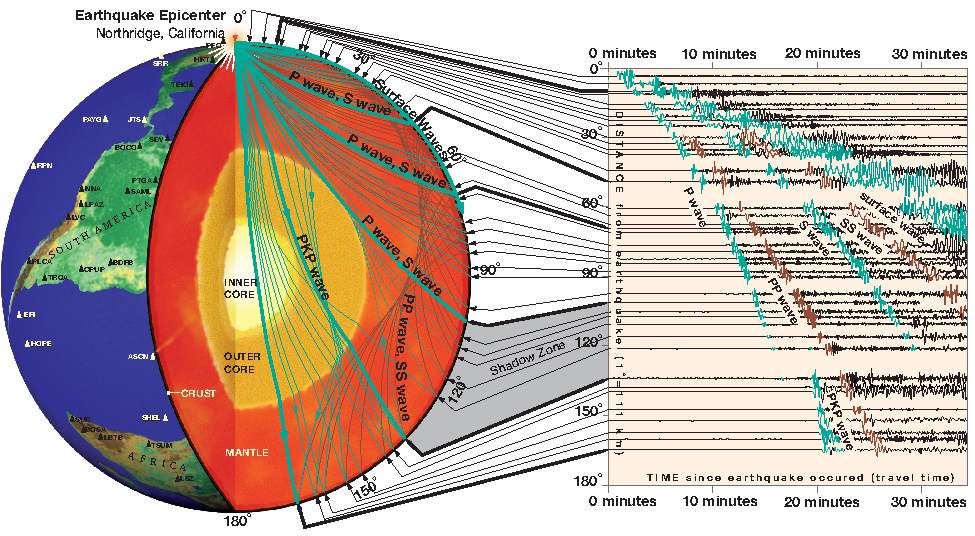
\includegraphics[width=0.8\textwidth]{figuras/ondas_p_s}
  \caption[Trayectorias y tiempos de viaje de las ondas P y S a través del interior de la Tierra \citep{iris2010seismology}]{\textbf{Trayectorias y tiempos de viaje de las ondas sísmicas a través del interior de la Tierra para el terremoto de Northridge (California, 17 de enero de 1994, $M_w$ 6.9).} Se muestran los caminos seguidos por las ondas P, S, PP, SS, PKP y superficiales al atravesar las diferentes capas terrestres; se aprecia la \textit{shadow zone} entre los $100^{\circ}$ y los $140^{\circ}$ donde las ondas P directas dejan de llegar al desviarse al atravesar el núcleo externo. También aparecen los sismogramas registrados en estaciones repartidas por el planeta, con la separación temporal creciente entre la llegada de las ondas P, S y superficiales en función de la distancia angular al epicentro \citep{iris2010seismology}.}
  \label{fig:ondas-ps}
\end{figure}

Estas dos tareas --detección de eventos y \textit{picking} preciso de las llegadas P/S-- han sido tradicionalmente abordadas por algoritmos heurísticos como STA/LTA (\textit{short-term average over long-term average}) y \textit{template matching} por correlación cruzada. Su limitación principal es la cantidad de falsos positivos en presencia de ruido o eventos solapados. El aprendizaje profundo ha desplazado en pocos años este campo mediante arquitecturas como PhaseNet \citep{zhu2018phasenet} y EQTransformer \citep{mousavi2020eqtransformer}, que se describen en la Sección \ref{dl-sismologia}.

\subsection{Ley de Gutenberg--Richter y \textit{b-value}}
\label{ley-gr}

La distribución de magnitudes en un catálogo sísmico sigue empíricamente una ley exponencial conocida como \emph{ley de Gutenberg--Richter} \citep{gutenberg1944frequency}, la cual relaciona la frecuencia de ocurrencia con la magnitud del terremoto:

\begin{equation}
  \log_{10} N(M) = a - b\, M,
  \label{eq:gr}
\end{equation}

donde $N(M)$ es el número de eventos con magnitud mayor o igual que $M$, $a$ caracteriza la productividad sísmica regional y $b$ es la pendiente, denominada \emph{b-value}, representa la relación entre sismicidad de pequeña y gran magnitud. Para regiones tectónicamente activas $b$ suele oscilar en torno a $1.0$ \citep{frohlich1993bvalues}, aunque variaciones temporales y espaciales del $b$-value tienen significado físico: $b$ es inversamente proporcional al estado de \emph{stress} acumulado en la corteza, de modo que decrementos transitorios del $b$-value preceden a algunos terremotos grandes \citep{schorlemmer2005bvalue}. Esta es precisamente una de las hipótesis precursoras que se evalúan en el capítulo \ref{desarrollo-del-proyecto-y-resultados}.

El estimador máximo verosímil del $b$-value es debido a \citet{aki1965bvalue}:
\begin{equation}
  \hat{b} = \frac{\log_{10}(e)}{\bar{M} - (M_c - \Delta M/2)},
  \label{eq:b-aki}
\end{equation}
con $\bar{M}$ la magnitud media de los eventos con $M \geq M_c$, $M_c$ la \emph{magnitud de completitud} del catálogo y $\Delta M$ el paso de discretización (típicamente $0.1$).

La Figura~\ref{fig:gr-cal-alaska} ilustra empíricamente la ley de Gutenberg--Richter sobre los catálogos USGS de California y Alaska (2010--2024). El ajuste sobre California (23\,322 eventos $M\geq 2.5$) arroja $b = 0.90$, valor que cae entre los regímenes de alto $\mathit{stress}$ ($b=0.8$ \citep{schorlemmer2005bvalue}) y el canónico global ($b=1.0$ \citep{frohlich1993bvalues}), coherente con un régimen tectónico transformante. Alaska (71\,026 eventos), por su parte, presenta $b = 0.74$, sensiblemente más bajo, lo que es consistente con un régimen de subducción donde se acumula proporcionalmente más sismicidad grande respecto a la pequeña \citep{wiemer2002mapping, frohlich1993bvalues}. La desviación de los datos respecto a la recta para magnitudes $M\gtrsim 6.5$ corresponde a los pocos eventos grandes registrados en el periodo y refleja la incertidumbre estadística esperada en la cola de la distribución.

\begin{figure}[ht!]
  \centering
  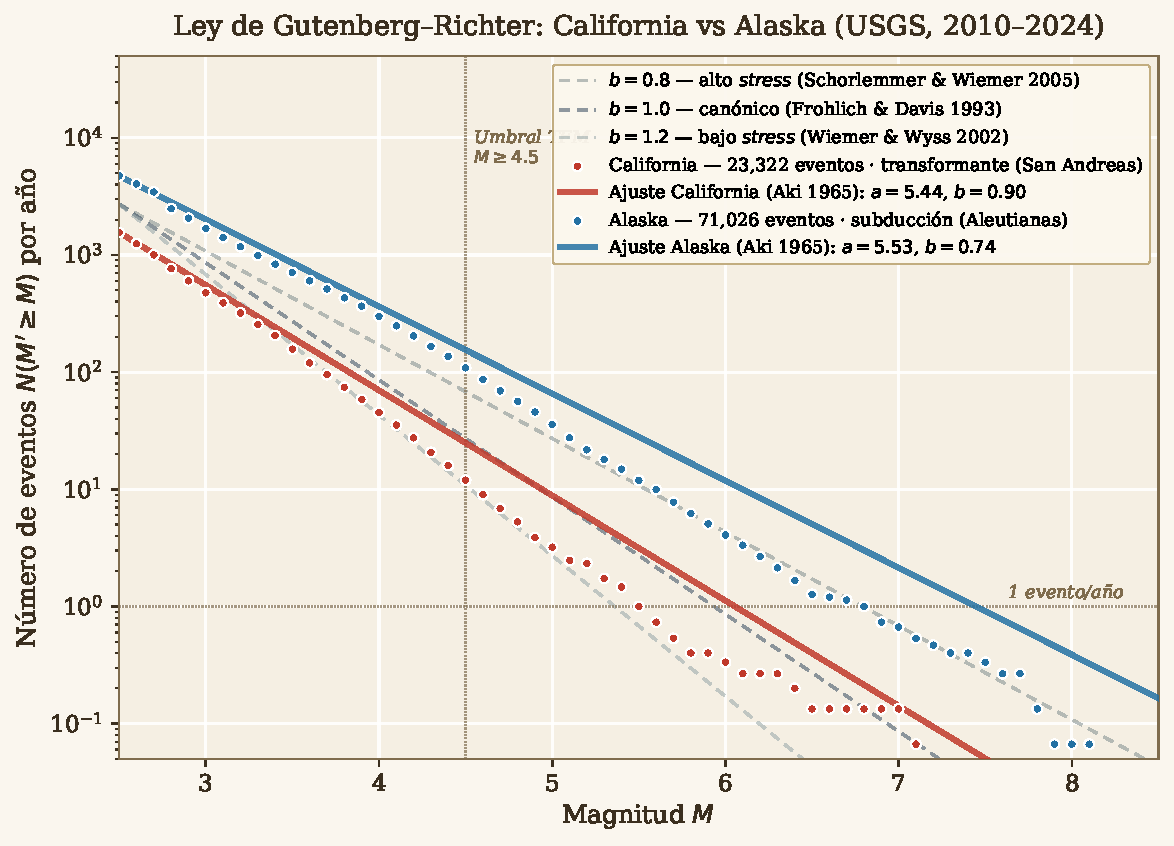
\includegraphics[width=0.95\textwidth]{figuras/figura_gr_california}
  \caption[Ley de Gutenberg--Richter empírica para California y Alaska (USGS 2010--2024)]{\textbf{Validación empírica de la ley de Gutenberg--Richter sobre los catálogos USGS de California y Alaska (2010--2024).} Los puntos representan la frecuencia acumulada anual de eventos por encima de cada magnitud; las líneas continuas son los ajustes máximo verosímiles obtenidos mediante el estimador de \citet{aki1965bvalue}, corregido por binning. Las líneas discontinuas grises muestran tres curvas teóricas de referencia con $b\in\{0.8, 1.0, 1.2\}$ correspondientes a distintos regímenes documentados en la literatura: alto $\mathit{stress}$ \citep{schorlemmer2005bvalue}, canónico global \citep{frohlich1993bvalues} y bajo $\mathit{stress}$ o volcánico \citep{wiemer2002mapping}. California (rojo) presenta $b = 0.90$, coherente con un régimen transformante (falla de San Andreas); Alaska (azul) presenta $b = 0.74$, valor más bajo característico de zonas de subducción (arco de las Aleutianas). Las líneas guía indican el umbral de pronóstico del TFM ($M\geq 4.5$, vertical) y la tasa de un evento al año (horizontal).}
  \label{fig:gr-cal-alaska}
\end{figure}

\subsection{Magnitud de completitud \texorpdfstring{$M_c$}{Mc}}
\label{mc}

La magnitud de completitud $M_c$ es el mínimo valor de $M$ a partir del cual el catálogo se considera estadísticamente completo (no faltan eventos por debajo del umbral de detección de la red de estaciones). Su determinación es un paso preprocesado esencial: \textit{features} agregadas calculadas con $M < M_c$ contaminarían la señal con ruido de selección, y un $M_c$ mal estimado sesga directamente el $b$-value de la ecuación (\ref{eq:b-aki}). Los métodos más utilizados en la literatura son:

\begin{itemize}
  \item \textbf{\textit{Maximum curvature} (MAXC).} Define $M_c$ como el punto de máxima curvatura de la distribución frecuencia--magnitud, equivalente al pico del histograma no acumulado de magnitudes \citep{wiemer2000mc}. Es rápido y fiable pero tiende a \emph{subestimar} $M_c$ en distribuciones suavemente curvadas.
  \item \textbf{\textit{Best combination} (BC).} Variante de MAXC con un intervalo de confianza del 95\,\%, lo que reduce el sesgo a costa de mayor coste computacional \citep{wiemer2000mc}.
  \item \textbf{\textit{Goodness-of-fit test} (GFT) y \textit{b-value stability}.} Métodos clásicos basados en la bondad de ajuste de la recta de G--R por encima de cada candidato a $M_c$ \citep{mignan2012mc}.
  \item \textbf{\textit{Entire-magnitude-range method} (EMR).} El método más robusto actualmente disponible: ajusta simultáneamente un modelo de ley de potencia para la parte completa ($M \geq M_c$) y una función de detección probabilística para la parte incompleta ($M < M_c$), maximizando la verosimilitud conjunta \citep{woessner2005assessing}.
\end{itemize}

Para las redes modernas SCSN/NCSN (California) y AEC (Alaska), la literatura sitúa $M_c \approx 2.0$--$2.5$ a partir del año 2000 \citep{wiemer2000mc}. En este trabajo se adopta $M_c = 2.5$ como umbral conservador, lo que asegura completitud incluso en periodos puntuales de menor cobertura de la red.

\subsection{Ley de Omori--Utsu y réplicas}
\label{omori}

Inmediatamente después de un terremoto grande (denominado \emph{mainshock}), se observa una secuencia de eventos menores --las \emph{réplicas} o \textit{aftershocks}-- cuya tasa de ocurrencia decae con el tiempo según la ley de \citet{omori1894aftershocks}, modificada posteriormente por \citet{utsu1961statistical}:
\begin{equation}
  n(t) = \frac{K}{(t + c)^p},
  \label{eq:omori}
\end{equation}
donde $K$, $c$ y $p$ son parámetros ajustables, siendo $p$ el que describe la tasa de decaimiento. Para California, $p$ se sitúa típicamente entre $0.9$ y $1.3$. La existencia de réplicas tiene una consecuencia metodológica crítica para los modelos de pronóstico: si un catálogo no se \emph{declusteriza}, los eventos no son independientes y cualquier modelo aprenderá a predecir trivialmente la continuación de una secuencia de réplicas, no patrones precursores reales \citep{vanstiphout2012declustering}.

\subsection{\textit{Declustering}: el algoritmo de Gardner--Knopoff}
\label{declustering}

El algoritmo de \citet{gardner1974poissonian} es la técnica de \textit{declustering} más utilizada históricamente. Para cada evento candidato a \textit{mainshock}, define una ventana espacio-temporal alrededor en la que cualquier evento de menor magnitud se considera réplica o \textit{foreshock} dependiente. Las ventanas de Gardner–Knopoff originalmente se publicaron como tabla; \citet{vanstiphout2012declustering} dan la versión continua que se usará en este trabajo:
\begin{align}
  L(M) & = 10^{0.1238\, M + 0.983}\,\,\mathrm{km} \label{eq:gk-L}                   \\
  T(M) & = 10^{0.5409\, M - 0.547}\,\,\text{días}, \quad M \geq 6.5 \label{eq:gk-T}
\end{align}
con una expresión alternativa para $M < 6.5$. Tras el filtrado se obtiene un sub-catálogo de \emph{mainshocks independientes} sobre el que se define el \emph{target} del problema de pronóstico. \citet{reasenberg1985declustering} propuso una variante posterior basada en una ventana modificada de Omori; ambas se consideran válidas en la literatura. La elección de G-K en este trabajo se justifica por su simplicidad, su naturaleza determinista (mismo catálogo entrada $\Rightarrow$ mismo catálogo salida, sin parámetros estocásticos) y su uso extendido como referencia comparativa.

\subsection{Catálogos sísmicos: USGS, SCSN, AEC y catalogos relocados}
\label{catalogos}

El \gls{usgs} mantiene un catálogo sísmico global accesible vía el web service FDSN, que agrega contribuciones de las redes regionales SCSN, NCSN, AEC y otras. Para estudios de más alta precisión existen catálogos relocados mediante métodos de diferencia doble (\textit{double-difference}): el de \citet{hauksson2012relocated} cubre el sur de California desde 1981, y el de \citet{waldhauser2008doubledifference} el norte. Estos catálogos relocados reducen el error de localización por un factor $\sim 10\times$ a costa de cobertura geográfica más restringida; en este TFM se utiliza el catálogo USGS bruto como fuente principal por homogeneidad regional, dejando los relocados como plan B para futuros trabajos.

\section{Métodos estadísticos clásicos de pronóstico sísmico}
\label{metodos-estadisticos-clasicos}

\subsection{De la predicción determinista al pronóstico probabilístico}
\label{prediccion-vs-pronostico}

Desde la década de los 70 hasta los años 90, sucesivos intentos de predicción sísmica determinista (lugar + tiempo + magnitud) resultaron en notorios fracasos, hasta el punto de que \citet{geller1997unpredictable} sintetizó en \textit{Science} la postura mayoritaria de la comunidad: ``los terremotos no pueden predecirse'', en el sentido del determinismo clásico. \citet{jordan2011oef} formalizaron la transición al \emph{pronóstico probabilístico}: en lugar de afirmar que un evento ocurrirá, se estima la probabilidad condicional $P(M \geq M^* \mid \text{\emph{historia}}, \text{\emph{ventana}}, \text{\emph{región}})$. Esto se ha materializado en sistemas operativos como \emph{Operational Earthquake Forecasting} en Italia \citep{marzocchi2014oef} y como el modelo UCERF3 en California \citep{field2014ucerf3, field2017ucerf3etas}. Ambos sistemas se articulan en torno a un mismo motor estadístico, el modelo \emph{Epidemic-Type Aftershock Sequence} (ETAS), que constituye la pieza central de la sismología probabilística clásica.

\subsection{El modelo UCERF3 y \textit{ShakeMap}}
\label{ucerf-shakemap}

El \emph{Uniform California Earthquake Rupture Forecast version 3} \citep{field2014ucerf3} integra geometría de fallas, tasas de deslizamiento geológicas, parámetros ETAS y modelos de propagación para producir mapas de peligrosidad probabilística a 30 días, 1 año, 30 años y 100 años. Su variante UCERF3-ETAS \citep{field2017ucerf3etas} añade la dimensión temporal corta. La Figura~\ref{fig:ucerf3-map} muestra el mapa resultante de UCERF3 para California, donde el color de cada segmento de falla codifica la probabilidad de participación en una ruptura sísmica de gran magnitud. Por su parte, \emph{ShakeMap} \citep{wald1999shakemap} es la herramienta operacional de generación de mapas de intensidad inmediatamente después de un evento. Estos sistemas constituyen el \textit{ground truth} operacional contra el que cualquier modelo de aprendizaje profundo aspira a competir o complementar.

\begin{figure}[ht!]
  \centering
  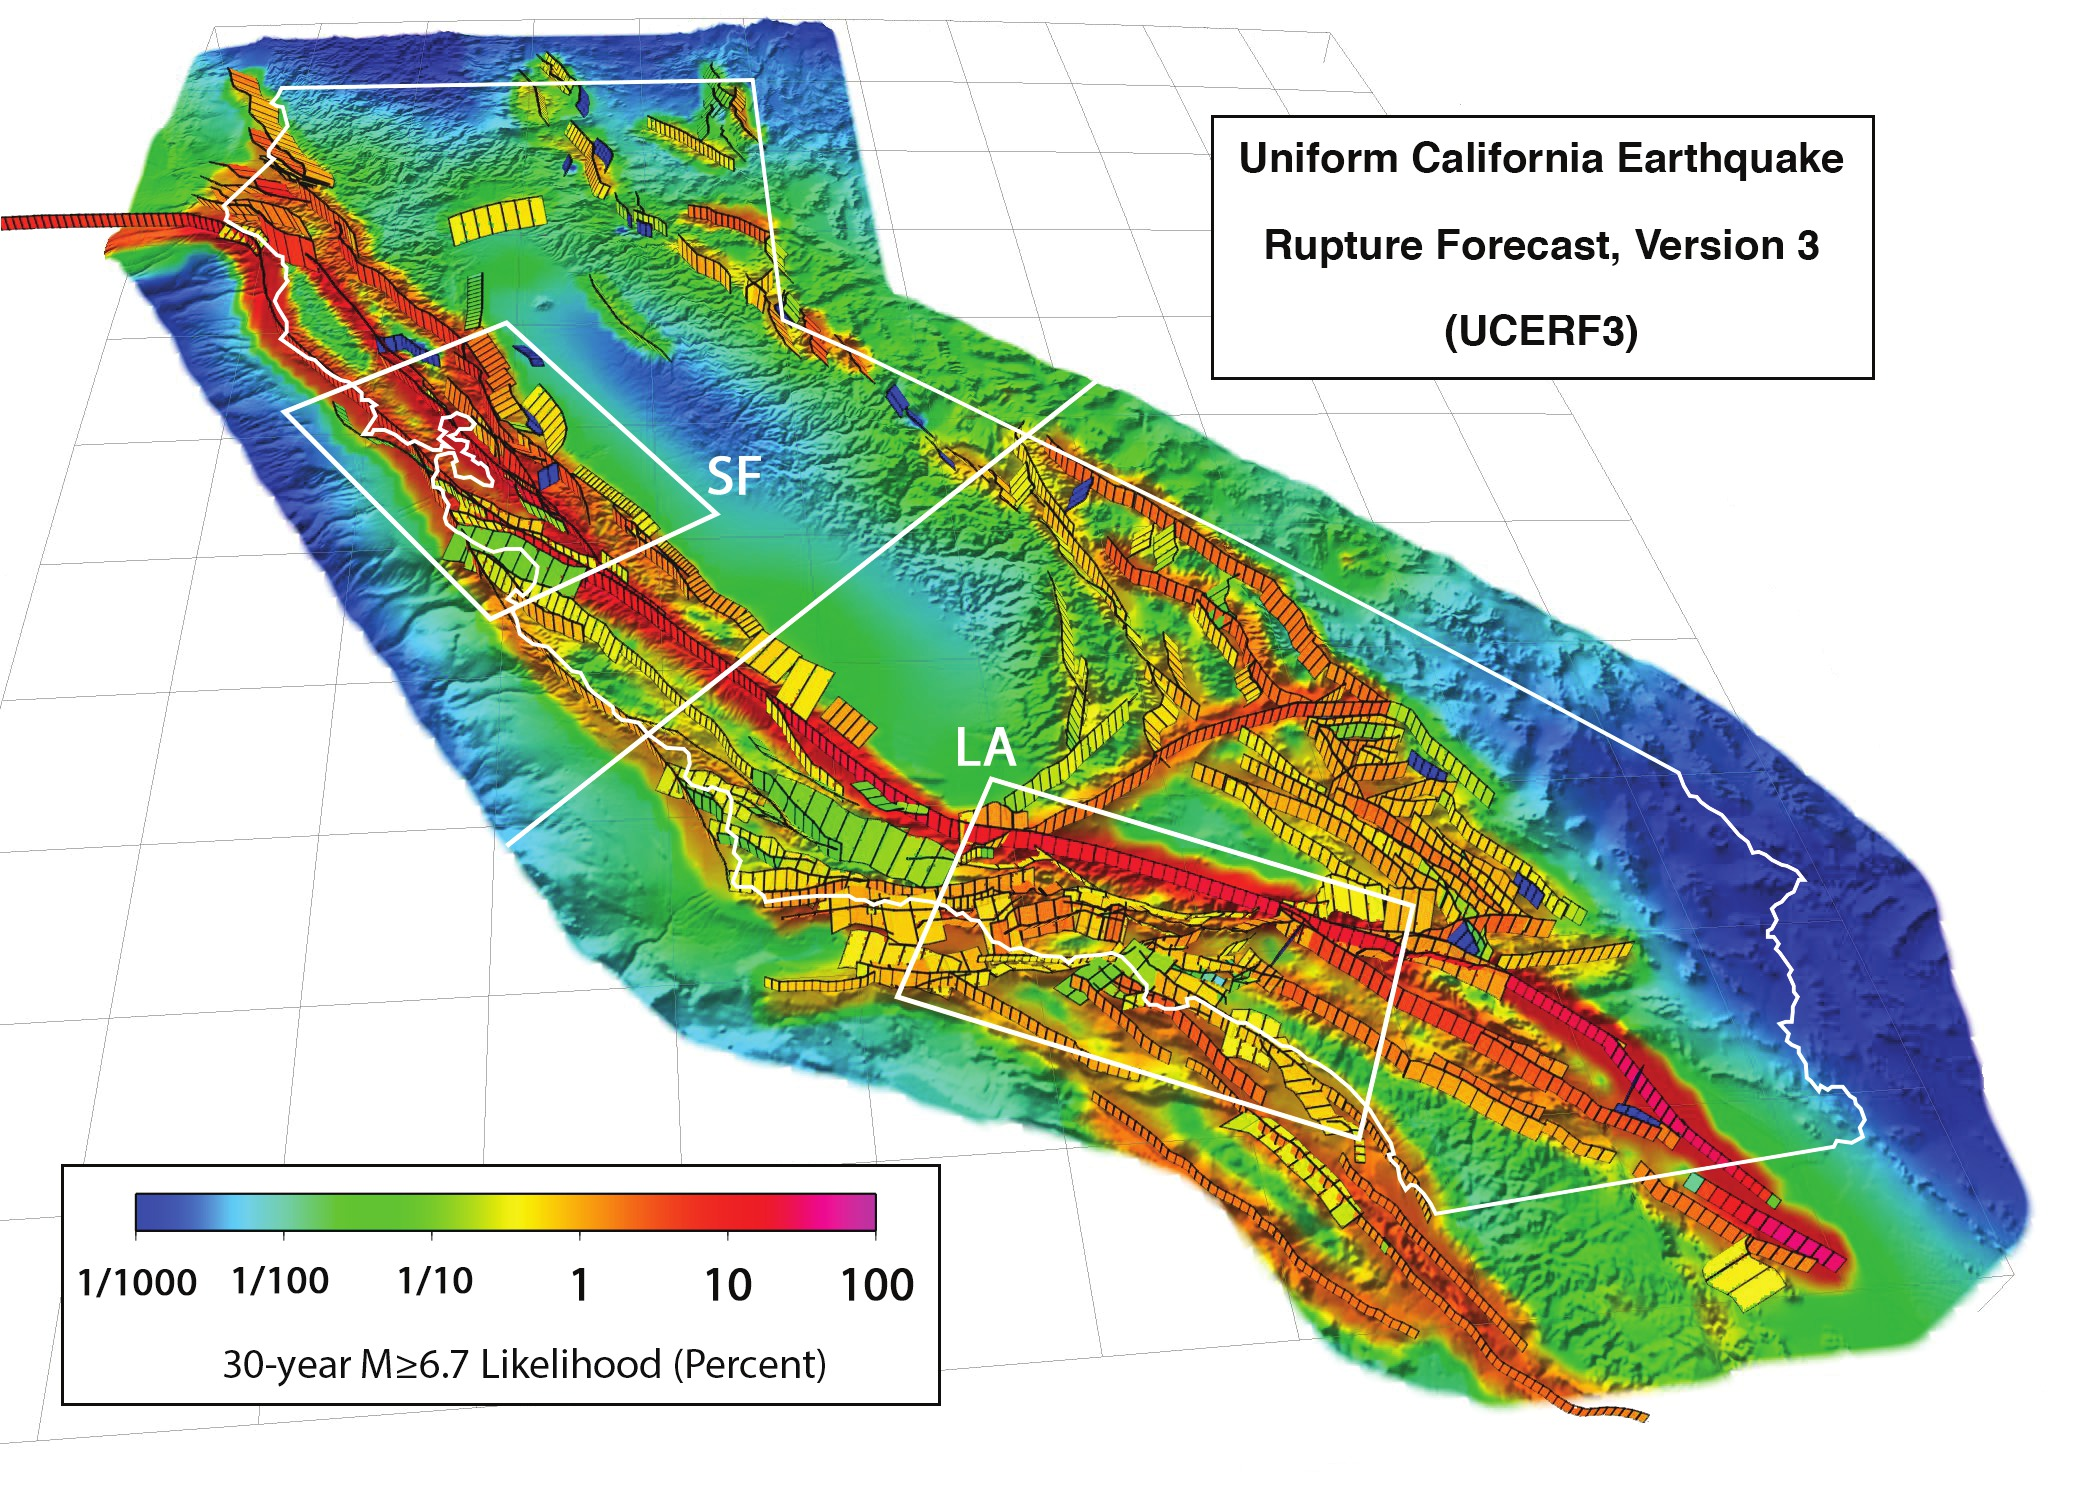
\includegraphics[width=0.85\textwidth]{figuras/figura_UCERF3.png}
  \caption[Mapa UCERF3 de probabilidad de terremoto $M\geq 6.7$ a 30 años en California \citep{wikipediaucerf3, field2015ucerf3factsheet}]{\textbf{Mapa UCERF3 de probabilidad de ocurrencia de un terremoto de $M\geq 6.7$ en los próximos 30 años en California.} El color de cada segmento de falla indica la probabilidad con la que esa sección participará en una ruptura sísmica de dicha magnitud; la falla de San Andrés y la de Hayward concentran las probabilidades más elevadas. El modelo integra geometría de fallas, tasas de deslizamiento geológicas y parámetros ETAS \citep{field2015ucerf3factsheet}. Imagen tomada del artículo divulgativo de Wikipedia sobre UCERF3 \citep{wikipediaucerf3}, prácticamente idéntica a la publicada en el \emph{fact sheet} oficial del USGS \citep{field2015ucerf3factsheet}.}
  \label{fig:ucerf3-map}
\end{figure}

\subsection{La familia ETAS}
\label{etas}

El \emph{Epidemic-Type Aftershock Sequence} de \citet{ogata1988etas, ogata1998spacetime} modela la sismicidad como un proceso de puntos auto-excitante: cada evento incrementa transitoriamente la tasa de ocurrencia en su entorno, con la tasa total $\lambda(t, x, y)$ formulada como
\begin{equation}
  \lambda(t,x,y) = \mu(x,y) + \sum_{i: t_i < t} \frac{K_0\, e^{\alpha(M_i - M_c)}}{(t - t_i + c)^p}\, f(x - x_i, y - y_i; M_i)
  \label{eq:etas}
\end{equation}
donde $\mu(x,y)$ es la tasa de fondo, el sumatorio recorre los eventos anteriores, y $f(\cdot)$ es un \textit{kernel} espacial isotrópico que decae con la distancia. Los parámetros $(K_0, \alpha, c, p)$ se ajustan por máxima verosimilitud sobre el catálogo. Sus virtudes: forma funcional interpretable, parámetros con significado físico, y posibilidad de generar muestras estocásticas vía simulación de \textit{branching process} (un proceso de ramificación que modela cómo un sismo principal desencadena sucesivas generaciones de réplicas). Sus limitaciones: forma del \textit{kernel} fija, dependencia exclusiva de metadatos de catálogo (sin uso del contenido de forma de onda), y dificultad para incorporar covariables externas (estrés de Coulomb, \textit{slow-slip events}, anomalías electromagnéticas, etc.). El sistema integrado UCERF3-ETAS \citep{field2017ucerf3etas} es el referente operacional clásico.

\section{Aprendizaje profundo: fundamentos generales}
\label{dl-fundamentos}

\subsection{Marco general y notación}

Una red neuronal profunda es una función $f_\theta: \mathbb{R}^d \to \mathbb{R}^k$ parametrizada por $\theta \in \mathbb{R}^p$ y construida por composición de transformaciones afines y no linealidades:
\begin{equation}
  f_\theta(x) = \phi_L \circ T_L \circ \phi_{L-1} \circ T_{L-1} \circ \cdots \circ \phi_1 \circ T_1(x),
\end{equation}
donde $T_\ell(z) = W_\ell\, z + b_\ell$ es una transformación afín y $\phi_\ell$ una función no lineal (ReLU, GELU, etc.). El entrenamiento consiste en minimizar una función de pérdida $\mathcal{L}(\theta) = \tfrac{1}{N}\sum_i \ell(f_\theta(x_i), y_i)$ sobre un dataset $\{(x_i, y_i)\}_{i=1}^N$, típicamente mediante descenso de gradiente estocástico. La obra de referencia es \citet{goodfellow2016deep}; un resumen accesible es \citet{lecun2015deep}.

\subsection{Optimizador Adam}

El optimizador más utilizado en aprendizaje profundo actual es \emph{Adam} \citep{kingma2015adam}, que combina momentos de primer y segundo orden con corrección de sesgo:
\begin{align}
  m_t      & = \beta_1 m_{t-1} + (1 - \beta_1)\, g_t,                              \\
  v_t      & = \beta_2 v_{t-1} + (1 - \beta_2)\, g_t^2,                            \\
  \theta_t & = \theta_{t-1} - \eta\, \hat{m}_t / (\sqrt{\hat{v}_t} + \varepsilon),
\end{align}
con $\hat{m}_t = m_t/(1 - \beta_1^t)$ y $\hat{v}_t = v_t/(1 - \beta_2^t)$. Los valores por defecto $(\beta_1, \beta_2, \varepsilon) = (0.9, 0.999, 10^{-8})$ son los usados en este trabajo.

\subsection{Regularización y \textit{dropout}}

Dado que los datasets en sismología son a menudo limitados en el dominio temporal (decenas de años), la regularización es crítica. Las técnicas usadas en este trabajo son \textit{weight decay} ($L_2$ sobre los pesos), \textit{dropout} (apagado aleatorio de unidades durante el entrenamiento) y \textit{early stopping} (detención temprana del entrenamiento del modelo) basado en la métrica de validación. El \textit{dropout} tiene además una segunda interpretación bayesiana \citep{gal2016mcdropout} que permite cuantificar incertidumbre por \textit{Monte Carlo dropout}, aunque en este trabajo la cuantificación de incertidumbre se delega a un \gls{gp} explícito (Sección \ref{dl-incertidumbre}).

\begin{figure}[ht!]
  \centering
  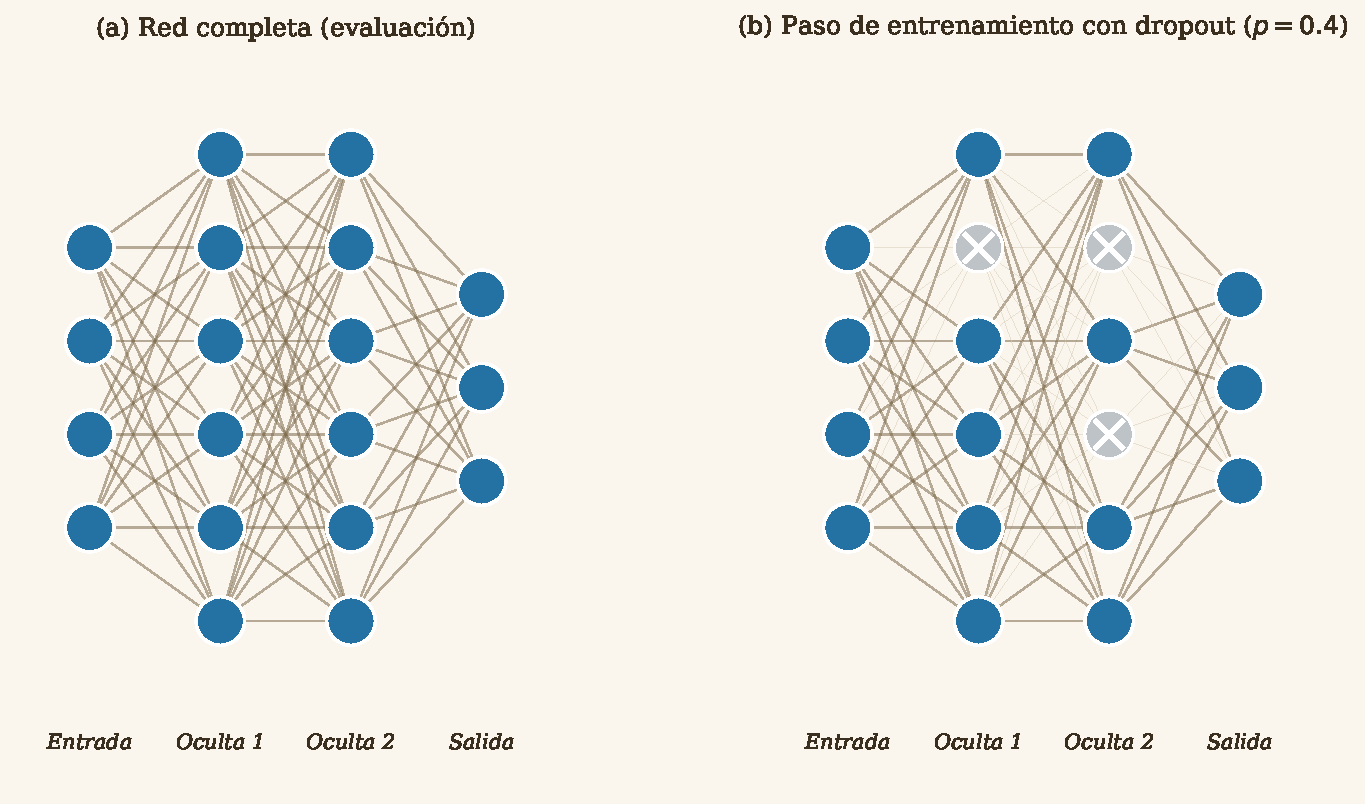
\includegraphics[width=0.95\textwidth]{figuras/figura_dropout}
  \caption[Mecanismo de \textit{dropout} durante el entrenamiento]{\textbf{Mecanismo de \textit{dropout} durante el entrenamiento.} (a) Red neuronal completa (\textit{fully connected}) durante la fase de inferencia o evaluación, donde todas las unidades están activas. (b) La misma red durante un paso de entrenamiento con \textit{dropout} ($p=0.4$); un subconjunto aleatorio de neuronas (en gris claro) y sus conexiones asociadas se desactivan. Esto obliga a la red a aprender representaciones más robustas y redundantes, reduciendo significativamente el sobreajuste.}
  \label{fig:dropout}
\end{figure}

\subsection{Desbalance de clases: \textit{pos\_weight} y \textit{Focal Loss}}
\label{desbalance}

El pronóstico sísmico es un problema fuertemente desbalanceado: en California y Alaska entre 2000 y 2024, sólo el $\sim 30\%$ de los días tienen al menos un \textit{mainshock} $M\geq 4.5$ en los siguientes \(30\) días; en una formulación por celda el ratio cae a $\sim 2\%$ \citep{he2009imbalanced}. Para mitigarlo se utiliza:
\begin{enumerate}
  \item \textbf{Ponderación de clase} (\textit{pos\_weight} en \texttt{BCEWithLogitsLoss}): asigna un peso $w_+ = N_-/N_+$ a la clase minoritaria.
  \item \textbf{\textit{Focal Loss}} \citep{lin2017focal}: \(\mathrm{FL}(p_t) = -\alpha_t\, (1 - p_t)^\gamma\, \log p_t\), que reduce el peso de los ejemplos fáciles ($p_t$ cercano a 1) y enfatiza los difíciles. Con $\gamma=2$ se obtiene típicamente mejor desempeño en problemas con desbalance fuerte.
\end{enumerate}

\section{Arquitecturas para series temporales}
\label{dl-temporal}

\subsection{Redes recurrentes y LSTM}

Las redes recurrentes (\gls{rnn}) procesan secuencias actualizando un estado oculto a cada paso temporal. La variante \emph{Long Short-Term Memory} (\gls{lstm}) de \citet{hochreiter1997lstm} introduce un mecanismo de \textit{gates} (\textit{forget gate}, \textit{input gate}, \textit{output gate}) que mitiga el problema del gradiente desvaneciente, permitiendo aprender dependencias de varias decenas a centenas de pasos. Han sido la arquitectura dominante en series temporales durante la década 2010--2020. Sus limitaciones --paralelización difícil, \textit{receptive field} efectivo limitado-- motivan las alternativas que se discuten a continuación.

\subsection{Temporal Convolutional Networks}
\label{tcn-marco}

Las \emph{Temporal Convolutional Networks} (\gls{tcn}), introducidas por \citet{bai2018tcn}, sustituyen la recurrencia por una pila de convoluciones 1D \emph{causales} y \emph{dilatadas} con conexiones residuales. Sus tres características definitorias son:

\begin{itemize}
  \item \textbf{Causalidad:} la salida en el tiempo $t$ depende solamente de las entradas en $t' \leq t$ (la convolución está desplazada para no usar el futuro).
  \item \textbf{Dilataciones exponenciales:} la $\ell$-ésima capa usa dilatación $d_\ell = 2^{\ell - 1}$, lo que permite un \emph{receptive field} (RF) que crece exponencialmente con la profundidad según
        \begin{equation}
          \mathrm{RF} = 1 + 2\,(K-1)\,(2^L - 1),
          \label{eq:rf-tcn}
        \end{equation}
        donde $K$ es el tamaño del \textit{kernel} y $L$ el número de capas. Para $K=3$, $L=4$ se obtiene RF $=61$, que cubre una ventana de aproximadamente dos meses (con resolución diaria) y motiva la elección del \texttt{LOOKBACK $=60$ días} en este trabajo.
  \item \textbf{Bloques residuales:} cada bloque añade un atajo $h \mapsto h + \mathrm{conv}(h)$ que facilita el entrenamiento de redes profundas.
\end{itemize}

Se mostraron empíricamente que las TCN igualan o superan a las LSTM en una amplia batería de benchmarks de modelado de secuencias (véase Tabla~\ref{tab:tcn-vs-lstm} en el Anexo~\ref{anexo-tcn-lstm}), con la ventaja adicional de la paralelización por GPU. Esto las hace candidatas naturales para modelar series temporales de sismicidad con resolución diaria, como se hace en el capítulo \ref{desarrollo-del-proyecto-y-resultados}.

\begin{figure}[ht!]
  \centering
  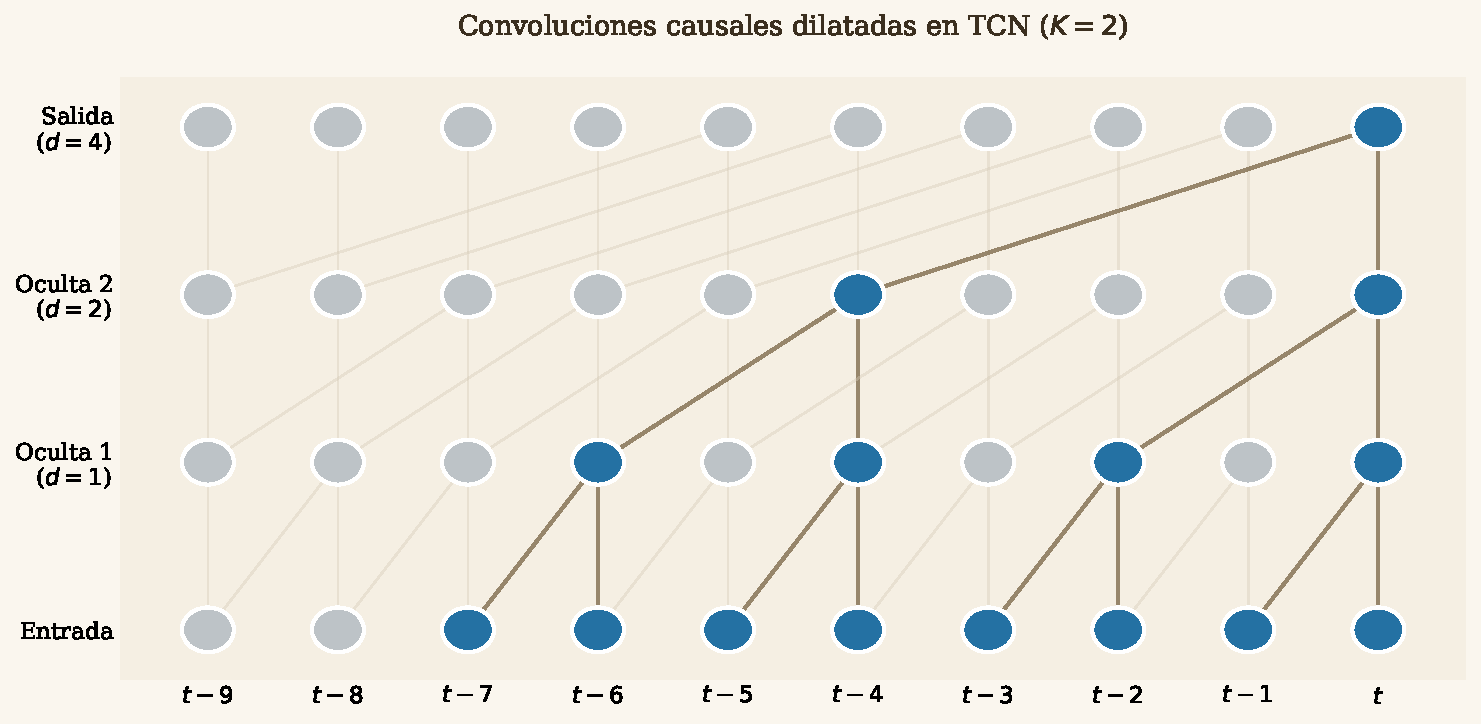
\includegraphics[width=0.9\textwidth]{figuras/figura_tcn}
  \caption[Arquitectura de una \textit{Temporal Convolutional Network} (TCN)]{\textbf{Convoluciones causales dilatadas en una TCN.} Ilustración del mecanismo para $K=2$ y dilataciones $d=\{1, 2, 4\}$. La causalidad asegura que no haya fuga de información del futuro, y las dilataciones exponenciales permiten que el \textit{receptive field} crezca rápidamente con la profundidad de la red, capturando dependencias a largo plazo de manera eficiente. Figura inspirada en \citet{bai2018tcn}.}
  \label{fig:tcn}
\end{figure}

\subsection{Mecanismo de atención y Transformers}

\citet{vaswani2017attention} propusieron el \emph{Transformer}, basado íntegramente en \emph{atención} sobre la secuencia sin recurrencia ni convolución. El cálculo de la atención mediante producto punto escalar se define como
\begin{equation}
  \mathrm{Attn}(Q, K, V) = \mathrm{softmax}\!\left(\frac{QK^\top}{\sqrt{d_k}}\right) V,
  \label{eq:attention}
\end{equation}
donde $Q, K, V$ son las proyecciones \emph{query, key, value} de la entrada. Su capacidad para modelar dependencias arbitrariamente largas en paralelo lo ha convertido en la arquitectura dominante en el procesamiento del lenguaje natural (NLP), la visión y, más recientemente, la sismología (EQTransformer \citep{mousavi2020eqtransformer}). En este trabajo se utiliza tanto el Transformer indirectamente (vía EQTransformer preentrenado en el notebook 02) como directamente bajo la forma de \emph{Transformer con codificación geoespacial} sobre la red de celdas activas.

\section{Arquitecturas para datos estructurados en grafo}
\label{dl-grafos}

\subsection{Motivación geofísica}

La sismicidad regional tiene una estructura espacial naturalmente representable como grafo: cada estación (o cada celda de discretización) es un nodo, y existen \emph{relaciones} físicamente significativas entre nodos cercanos (transferencia de estrés de Coulomb, propagación de ondas, conectividad de fallas). Las \gls{gnn} \citep{scarselli2009gnn} generalizan el operador convolucional a grafos arbitrarios y son por tanto la arquitectura natural para esta representación.

\subsection{Graph Convolutional Networks (GCN)}
\label{gcn-marco}

\citet{kipf2017gcn} introdujeron la \gls{gcn}, cuya capa se define como
\begin{equation}
  H^{(\ell+1)} = \sigma\!\left(\tilde{D}^{-\frac{1}{2}}\, \tilde{A}\, \tilde{D}^{-\frac{1}{2}}\, H^{(\ell)}\, W^{(\ell)}\right),
  \label{eq:gcn}
\end{equation}
donde $\tilde{A} = A + I$ es la matriz de adyacencia con autoaristas (\textit{self-loops}), $\tilde{D}$ su matriz de grados, $H^{(\ell)}$ las representaciones de los nodos en la capa $\ell$, $W^{(\ell)}$ los pesos aprendibles y $\sigma$ una no linealidad. La normalización simétrica $\tilde{D}^{-1/2}\tilde{A}\tilde{D}^{-1/2}$ asegura estabilidad numérica y un espectro acotado del operador de propagación.

El significado intuitivo es que cada nodo agrega información de sus vecinos inmediatos, ponderada por el grado, antes de aplicar una transformación lineal. Apilando $L$ capas, un nodo recibe información de su entorno $L$-saltos. En el modelo propuesto en el capítulo \ref{desarrollo-del-proyecto-y-resultados}, se utiliza una variante \emph{spatiotemporal} en la que una TCN comparte pesos entre celdas para procesar la dimensión temporal y a continuación dos capas GCN propagan información espacial entre celdas.

\subsection{Graph Attention Networks (GAT)}
\label{gat-marco}

\citet{velickovic2018gat} propusieron las \emph{Graph Attention Networks} (\gls{gat}), que sustituyen la ponderación fija del grado por una atención aprendible entre cada par de nodos vecinos:
\begin{equation}
  \alpha_{ij} = \frac{\exp\!\left(\mathrm{LeakyReLU}(\mathbf{a}^\top [W h_i \| W h_j])\right)}{\sum_{k \in \mathcal{N}(i)} \exp\!\left(\mathrm{LeakyReLU}(\mathbf{a}^\top [W h_i \| W h_k])\right)},
\end{equation}
donde $\mathbf{a}$ es un vector aprendible y $\|$ denota concatenación. GAT ofrece interpretabilidad (qué vecinos pesan más) a costa de un número mayor de parámetros. En este trabajo se utiliza GCN como arquitectura principal y se reserva GAT como ablation futura.

\subsection{Construcción del grafo: distancia de Haversine y \textit{KNN fallback}}

El grafo entre celdas activas se construye conectando pares cuya distancia de Haversine
\begin{equation}
  d(\mathbf{p}_1, \mathbf{p}_2) = 2 R\, \mathrm{arc\,sen}\!\left(\sqrt{\sin^2\!\tfrac{\Delta\varphi}{2} + \cos\varphi_1\,\cos\varphi_2\,\sin^2\!\tfrac{\Delta\lambda}{2}}\right),
  \label{eq:haversine}
\end{equation}
es menor que un umbral (\(100\) km en este trabajo). En la expresión, $\mathbf{p}_1$ y $\mathbf{p}_2$ son los centroides de las dos celdas; $\varphi$ denota la \emph{latitud} y $\lambda$ la \emph{longitud} de cada punto (en radianes), de modo que $\varphi_1,\varphi_2$ son las latitudes respectivas, $\Delta\varphi = \varphi_2 - \varphi_1$ la diferencia de latitud y $\Delta\lambda = \lambda_2 - \lambda_1$ la de longitud; $R$ es el radio medio de la Tierra ($\approx 6371$\,km). Para garantizar que ningún nodo quede aislado se aplica un \textit{fallback} basado en los K vecinos más cercanos (KNN, $k=2$) que conecta cada nodo a sus dos vecinos más cercanos aunque excedan el umbral. Esta combinación garantiza grado mínimo $\geq 2$ sin perder estructura física.

\subsection{Software: PyTorch Geometric}

La implementación de GNNs en este trabajo se apoya en \emph{PyTorch Geometric} \citep{fey2019pyg}, librería estandarizada para grafos sobre \emph{PyTorch} \citep{paszke2019pytorch}. PyG proporciona implementaciones eficientes de GCN, GAT y otros operadores, y simplifica la gestión de batches de grafos heterogéneos.

\section{Cuantificación de incertidumbre: Procesos Gaussianos}
\label{dl-incertidumbre}

Una predicción probabilística de riesgo sísmico tiene poca utilidad operativa si no viene acompañada de una estimación de su incertidumbre. Los \emph{Procesos Gaussianos} (\gls{gp}, \citep{rasmussen2006gp}) son un marco bayesiano no paramétrico ideal para esta tarea: definen una distribución de probabilidad sobre funciones $f \sim \mathcal{GP}(m, k)$, especificada por una función de media $m(\mathbf{x})$ y un \textit{kernel} de covarianza $k(\mathbf{x}, \mathbf{x}')$. Dado un conjunto de observaciones $\{(\mathbf{x}_i, y_i)\}$, la predicción posterior es nuevamente Gaussiana con media y varianza analíticas:
\begin{align}
  \mu_*(\mathbf{x}_*)      & = \mathbf{k}_*^\top (K + \sigma_n^2 I)^{-1} \mathbf{y},                                   \\
  \sigma_*^2(\mathbf{x}_*) & = k(\mathbf{x}_*, \mathbf{x}_*) - \mathbf{k}_*^\top (K + \sigma_n^2 I)^{-1} \mathbf{k}_*,
\end{align}
con $K_{ij} = k(\mathbf{x}_i, \mathbf{x}_j)$ y $\mathbf{k}_* = [k(\mathbf{x}_*, \mathbf{x}_i)]_i$. La elección del \textit{kernel} codifica las hipótesis a priori sobre la suavidad y la escala característica del fenómeno. Para datos sísmicos espaciales se utilizan típicamente \textit{kernels} de tipo Matérn con escalas de varios kilómetros.

En el sistema integrado propuesto, el GP recibe como entrada las probabilidades brutas $\hat{p}(\text{\emph{celda}}, \text{\emph{día}})$ generadas por la GNN y produce un campo suave $(\mu_*, \sigma_*)$ que constituye el mapa final de riesgo. Esto combina la potencia representacional del aprendizaje profundo (DL) con la estricta cuantificación bayesiana del GP.

\section{Mapas de peligrosidad y riesgo sísmico}
\label{mapas-riesgo}

\subsection{Peligro, exposición, vulnerabilidad y riesgo}
En el ámbito de la sismología aplicada y la ingeniería sísmica, resulta fundamental establecer una demarcación terminológica rigurosa entre cuatro conceptos interdependientes. El \emph{peligro sísmico} (\textit{seismic hazard}) denota la probabilidad de que ocurra un evento de cierta intensidad en un emplazamiento y periodo de tiempo definidos. La \emph{exposición} refiere al inventario de elementos físicos o humanos (población, infraestructuras) situados en la zona de afectación. La \emph{vulnerabilidad} cuantifica la susceptibilidad de dichos elementos a sufrir daños frente a un determinado nivel de sacudida. Finalmente, el \emph{riesgo sísmico} (\textit{seismic risk}) es la convolución matemática de los tres factores anteriores, estimando las pérdidas potenciales (económicas o humanas). El alcance computacional y metodológico de este TFM se centra exclusivamente en el modelado del \emph{peligro}, aunque sus resultados sirven de base fundamental para cualquier análisis de riesgo posterior.

\subsection{PSHA (\textit{Probabilistic Seismic Hazard Assessment}) vs. OEF}
La evaluación del peligro sísmico se ha regido históricamente por el paradigma PSHA, introducido formalmente por \citet{cornell1968engineering} y estandarizado metodológicamente por \citet{mcguire1995probabilistic}. Este enfoque clásico persigue la estimación probabilística de la tasa de excedencia de diferentes niveles de aceleración del terreno a largo plazo (típicamente horizontes de 50 años), asumiendo un modelo estadístico subyacente de Poisson (es decir, una tasa de sismicidad constante e independiente de la historia reciente).

En contraste directo con esta perspectiva estática a largo plazo, el Pronóstico Operacional de Terremotos (\textit{Operational Earthquake Forecasting}, OEF) \citep{jordan2011oef} aborda las fluctuaciones espaciotemporales dinámicas de la sismicidad a muy corto plazo (días o semanas). Dado que el marco temporal de predicción propuesto en este TFM opera sobre ventanas prospectivas de 30 días apoyadas en aprendizaje profundo, el sistema desarrollado se categoriza conceptualmente dentro del paradigma dinámico OEF, suplementando, pero no sustituyendo, a los mapas estáticos PSHA tradicionales.

\subsection{De probabilidad por celda a mapa continuo}
Los algoritmos de clasificación de aprendizaje automático, especialmente aquellos operando sobre una discretización espacial (rejilla o \textit{grid}), devuelven típicamente una variable de salida logística (pseudoprobabilidad) asociada al centroide de cada celda. Para que estas inferencias brutas adquieran la categoría de mapa de peligrosidad accionable, requieren dos etapas de posprocesamiento (véase la Figura~\ref{fig:mapa-riesgo}).

En primera instancia, las puntuaciones deben ser calibradas probabilísticamente para asegurar que reflejan tasas de ocurrencia empíricas reales. Métodos de calibración como el escalado de Platt \citep{platt1999probabilistic} o la regresión isotónica mapean las salidas de los márgenes del clasificador hacia probabilidades matemáticas condicionales estrictas. En segunda instancia, el mapa de probabilidades por celda discreta debe ser interpolado espacialmente (e.g., \textit{kriging} universal). Es en esta etapa de interpolación topológica continua donde los Procesos Gaussianos (véase \ref{dl-incertidumbre}) evidencian su utilidad práctica, generando una superficie analítica suave que incluye bandas de confianza para cada coordenada geoespacial.

\begin{figure}[ht!]
  \centering
  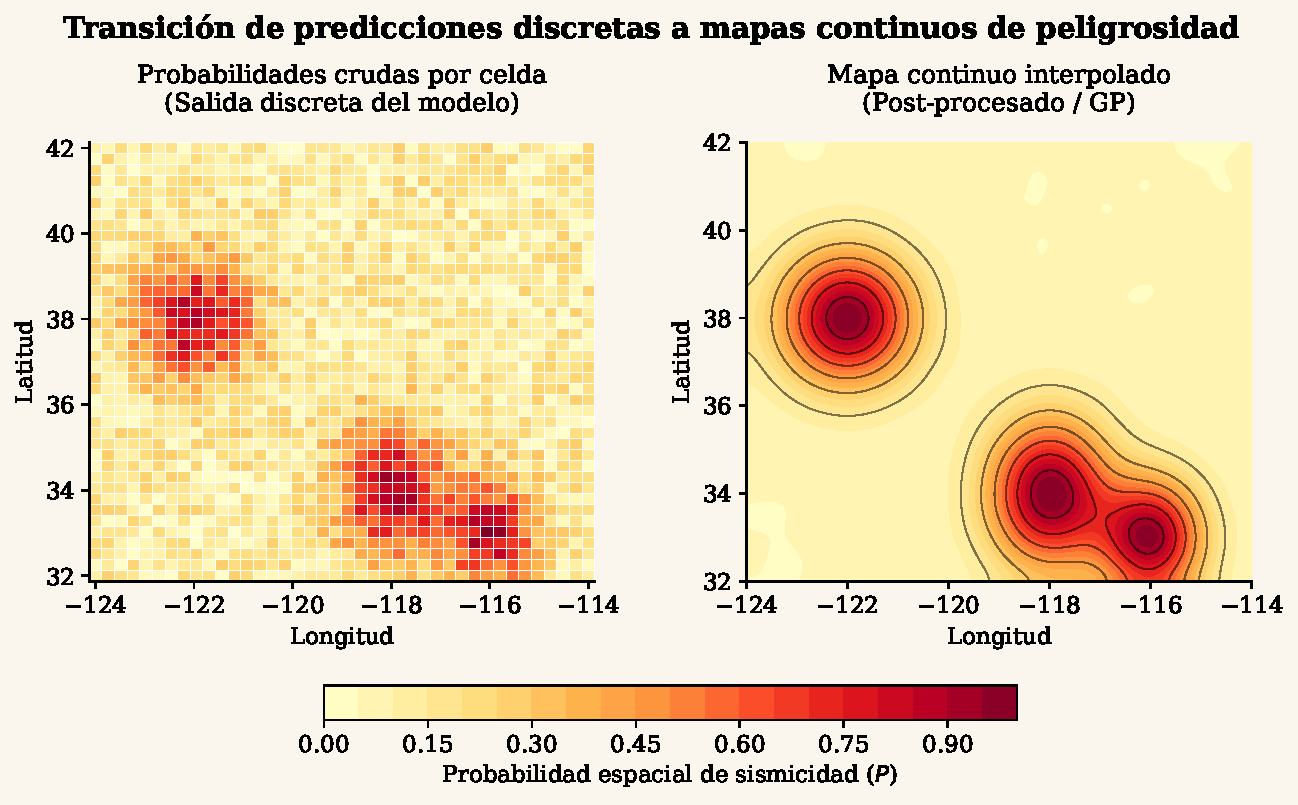
\includegraphics[width=0.9\textwidth]{figuras/figura_mapa_riesgo}
  \caption[Transición de predicciones discretas a mapas continuos de peligrosidad]{\textbf{Transición de predicciones discretas a mapas continuos de peligrosidad.} Izquierda: Probabilidades brutas (\textit{raw}) emitidas por un modelo de inferencia operando sobre una partición espacial discreta. Derecha: Superficie de peligrosidad interpolada mediante posprocesamiento espacial continuo (e.g., Procesos Gaussianos), donde se delinean isolíneas que demarcan frentes equiprobables, un formato mucho más asimilable para la gestión de emergencias.}
  \label{fig:mapa-riesgo}
\end{figure}

\subsection{Visualización y comunicación}
El diseño de mapas de riesgo sísmico debe priorizar la claridad y facilidad de comprensión tanto para los gestores de protección civil como para el público general. Herramientas de referencia en la ingeniería geofísica como \emph{ShakeMap} \citep{wald1999shakemap} han fijado los estándares en el uso de paletas de color y curvas de nivel (isolíneas) para representar con precisión la intensidad del movimiento del suelo. Asimismo, proyectos centrados en fallas a gran escala, como el modelo californiano UCERF3 \citep{field2014ucerf3}, basan sus metodologías de difusión en este mismo tipo de visualizaciones cartográficas. Este enfoque de comunicación transparente y estandarizada responde directamente a los principios éticos de difusión del riesgo promovidos por el Marco de Sendai \citep{un2015sendai}.

\section{Aprendizaje profundo aplicado a sismología}
\label{dl-sismologia}

\subsection{Detección y \textit{picking}: PhaseNet, EQTransformer y GPD}
\label{deteccion-picking}

\citet{zhu2018phasenet} introdujeron \emph{PhaseNet}, una U-Net 1D entrenada sobre $\sim 700\,000$ formas de onda etiquetadas para identificar y localizar las llegadas P y S. Cada traza de tres componentes a 100\,Hz se procesa por una red en forma de ``U'' con saltos simétricos y produce tres canales de salida: probabilidad de P, probabilidad de S y probabilidad de ruido. Sus errores de \textit{picking} son comparables a los de un analista humano y su \emph{recall} supera ampliamente al de los métodos heurísticos tipo STA/LTA.

\citet{mousavi2020eqtransformer} propusieron \emph{EQTransformer}, una red que ha pasado a ser una de las herramientas más usadas en sismología moderna. La idea principal es resolver tres tareas a la vez con un solo modelo: decir si hay un terremoto en el registro, marcar la llegada de la onda P y marcar la llegada de la onda S. Para ello combina tres ingredientes que ya habían funcionado por separado en otros trabajos pero que aquí se integran por primera vez:

\begin{enumerate}
  \item Una \textbf{parte convolucional} (CNN, \textit{Convolutional Neural Network}) que actúa como ``ojo'' inicial y extrae características locales del sismograma, parecido a cómo un humano se fija en la forma de los picos y los cambios bruscos.
  \item Una \textbf{parte recurrente bidireccional} (BiLSTM, \textit{Bidirectional LSTM}) que recorre la señal hacia delante y hacia atrás, recordando lo que ha pasado antes y después de cada instante para no descartar información que solo es útil al ver el contexto completo.
  \item Un \textbf{mecanismo de atención} de tipo \textit{Transformer} que aprende, por sí solo, qué fragmentos del sismograma son los más informativos para cada tarea y los ``ilumina'' frente al resto. Este es el componente que da nombre a la red y la diferencia de PhaseNet: en lugar de mirar la traza con la misma resolución en todas partes, el modelo decide dónde concentrar el cómputo.
\end{enumerate}

La red está entrenada sobre \gls{stead} con etiquetas precisas de llegada P y S, y devuelve tres canales de probabilidad sincronizados (detección, P, S) que se leen como funciones del tiempo. Cuando uno de esos canales supera un umbral configurable, se considera una predicción. En las pruebas originales sobre el propio STEAD y sobre datos no vistos de la red sísmica del norte de California, EQTransformer iguala o mejora a PhaseNet en \textit{recall} y comete menos falsos positivos en presencia de ruido o de eventos solapados, gracias al efecto regularizador del mecanismo de atención. Además, la versión preentrenada generaliza razonablemente bien a regiones distintas a las del entrenamiento. Por todas estas razones se ha convertido, junto con PhaseNet, en uno de los dos modelos de referencia para detección y \textit{picking} automáticos y es la única arquitectura que, en una sola pasada, cubre las tres tareas más comunes del pipeline sismológico.

\begin{figure}[ht!]
  \centering
  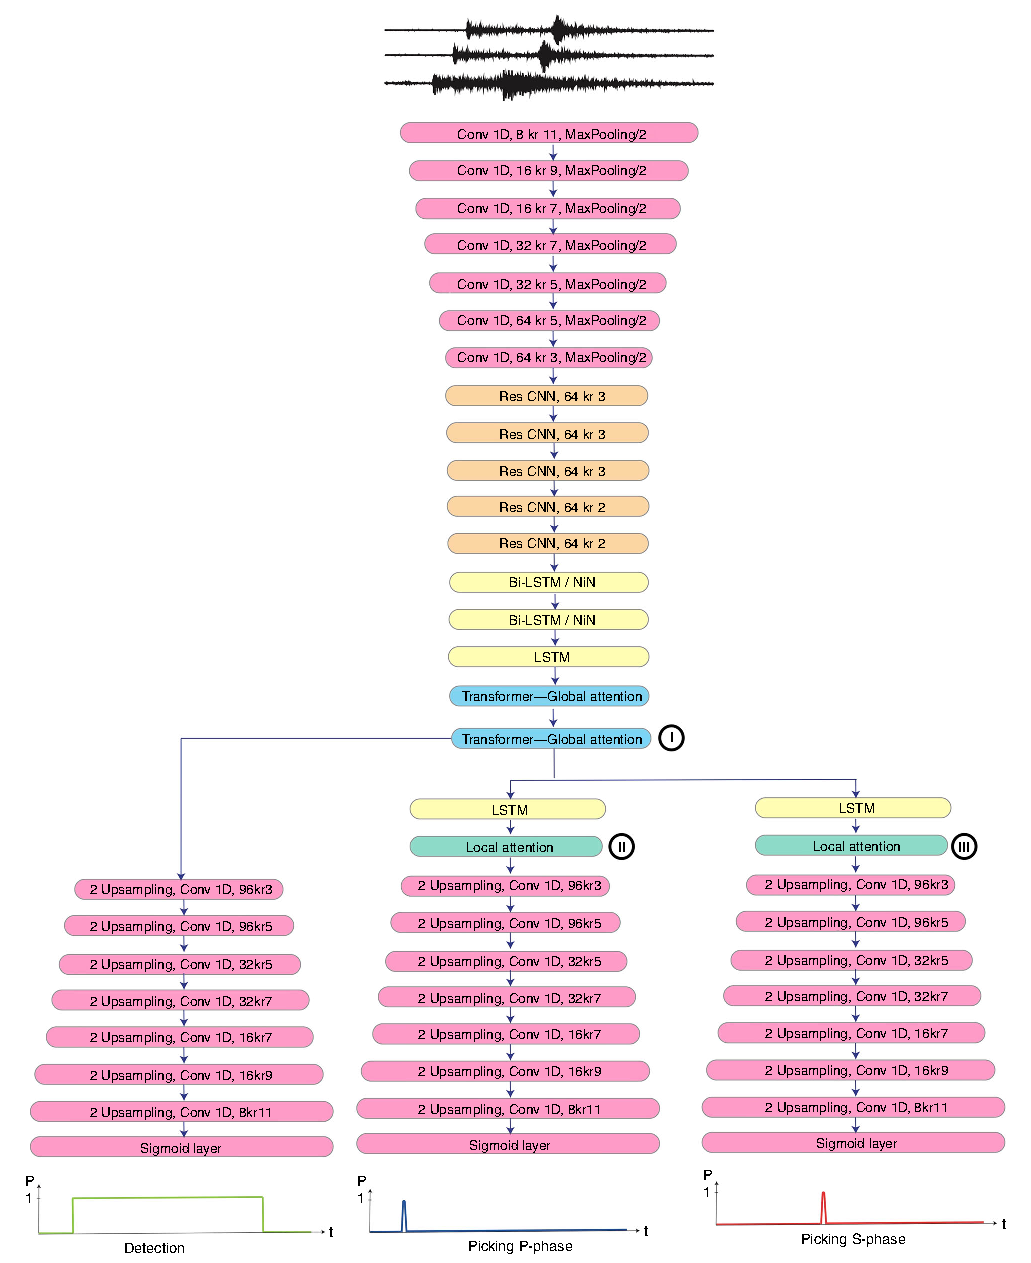
\includegraphics[width=0.8\textwidth]{figuras/figura_eqtransformer}
  \caption[Arquitectura de EQTransformer \citep{mousavi2020eqtransformer}]{\textbf{Arquitectura de EQTransformer \citep{mousavi2020eqtransformer}.} El sismograma de tres componentes (6000 muestras, 60\,s a 100\,Hz) entra por la parte superior y se procesa mediante bloques convolucionales y mecanismos de atención para detectar eventos sísmicos y estimar las llegadas de ondas P y S.}
  \label{fig:eqtransformer}
\end{figure}

Adicionalmente, \citet{ross2018generalized} mostraron con \emph{Generalized Phase Detection} (GPD) la viabilidad de una CNN simple entrenada en California que generaliza bien a otras regiones, y \citet{perol2018convnetquake} demostraron en \emph{Science Advances} que una CNN puede detectar y localizar simultáneamente eventos en Oklahoma. \citet{mousavi2019cred} añadieron \emph{CRED}, un modelo residual híbrido CNN + RNN para detección con baja relación señal-ruido (SNR). Todas estas arquitecturas están accesibles a través de \emph{SeisBench} \citep{woollam2022seisbench}, un toolkit estandarizado para aprendizaje automático (ML) en sismología que se usa en este trabajo (notebook 02).

\subsection{Pronóstico y detección de precursores}
\label{pronostico-precursores}

\citet{devries2018aftershocks} publicaron en \emph{Nature} una red densa que predice la distribución espacial de réplicas a partir de métricas de transferencia de estrés; aunque su evaluación inicial fue cuestionada posteriormente, abrió la línea de pronóstico espacial con DL. \citet{rouetleroy2017slowslip} aplicaron \emph{Random Forests} sobre señales acústicas en laboratorio para predecir deslizamientos en fallas controladas, mostrando que la señal estacional de \textit{slip} contiene información precursora explotable. \citet{vandenende2024forecasting} extendieron muy recientemente esta línea a \emph{deep neural temporal point processes} sobre catálogos reales, mostrando ganancias significativas sobre ETAS.

Para la \textbf{asociación de fases en redes densas}, \citet{mcbrearty2023gnn} desarrollaron una GNN específica que demuestra que la estructura de grafo natural de la red de estaciones puede explotarse para asociar correctamente picks pertenecientes al mismo evento, problema que tradicionalmente requería heurísticas complejas. Para la \textbf{caracterización automática de fuentes} (mecanismo focal, momento sísmico), \citet{vandenende2020tcnseismic} aplicaron GNNs sobre las formas de onda registradas en múltiples estaciones de la misma red.

\subsection{Revisiones del campo}

Las revisiones recientes más relevantes son \citet{kong2019mlseismology} en \emph{SRL}, \citet{beroza2021dlreview} en \emph{Nature Communications} y la más reciente \citet{mousavi2023review} en \emph{Annual Review of Earth and Planetary Sciences}. Las tres coinciden en señalar que el campo ha madurado en detección y \textit{picking} (PhaseNet/EQT como estándar de facto), pero todavía se encuentra en una fase inicial en pronóstico y predicción, donde la mayor parte de la mejora ha venido de un manejo más cuidadoso de los datos y los \textit{baselines} más que de cambios fundamentales de arquitectura.

\section{Métricas de evaluación en escenarios de desbalance extremo}
\label{metricas-desbalance}

\subsection{La paradoja del \textit{accuracy}}
\label{paradoja-accuracy}

En problemas de clasificación con clases muy desequilibradas, como el pronóstico sísmico, la métrica más intuitiva --el porcentaje de aciertos o \textit{accuracy}-- se vuelve engañosa. En este TFM, por ejemplo, los días con un \textit{mainshock} $M\geq 4.5$ en los siguientes 30 días representan en torno al 30\,\% del total a escala global y caen por debajo del 2\,\% cuando el problema se formula por celda. Un modelo que predijera ``no habrá terremoto'' de forma constante alcanzaría entre un 70 y un 98\,\% de \textit{accuracy} sin aportar nada útil. Para evitar esta trampa se utilizan métricas que separan los aciertos por clase y penalizan tanto los falsos positivos como los falsos negativos \citep{he2009imbalanced}.

\subsection{Precision, recall y F1-score}
\label{precision-recall-f1}

A partir de la matriz de confusión, con TP (verdaderos positivos), FP (falsos positivos), TN (verdaderos negativos) y FN (falsos negativos), se definen las dos métricas básicas
\begin{equation}
  \mathrm{Precision} = \frac{TP}{TP + FP}, \qquad \mathrm{Recall} = \frac{TP}{TP + FN}
  \label{eq:precision-recall}
\end{equation}
y su media armónica, el \textit{F1-score}
\begin{equation}
  F_1 = 2 \cdot \frac{\mathrm{Precision} \cdot \mathrm{Recall}}{\mathrm{Precision} + \mathrm{Recall}}
  \label{eq:f1}
\end{equation}

\textit{Recall} responde a la pregunta ``de los terremotos que realmente ocurrieron, ¿cuántos consiguió detectar el modelo?'', mientras que \textit{Precision} responde a ``de las alarmas que el modelo emitió, ¿cuántas correspondieron a un terremoto real?''. Ambas métricas están en tensión: subir el umbral de decisión mejora la \textit{Precision} a costa del \textit{Recall}, y viceversa. El F1-score resume el equilibrio entre las dos en un único número.

En un sistema operativo de pronóstico, qué métrica priorizar depende del coste relativo de cada tipo de error. Un alto \textit{Recall} es esencial cuando perderse un terremoto es inaceptable (alerta temprana en zonas pobladas), mientras que una alta \textit{Precision} se prefiere cuando las falsas alarmas tienen un coste social o económico relevante (evacuaciones, parones industriales).

\subsection{Curva Precision-Recall y PR-AUC}
\label{pr-auc}

La curva ROC, que enfrenta la tasa de verdaderos positivos contra la de falsos positivos, es la métrica más conocida en aprendizaje automático y la que reportamos como AUC en la sección de metodología. Sin embargo, cuando la clase positiva es muy minoritaria, la curva ROC tiene un sesgo bien documentado: la tasa de falsos positivos queda artificialmente baja porque el denominador (los negativos) es enorme, lo que hace que cualquier modelo deficiente produzca una curva visualmente convincente \citep{davis2006relationship, saito2015precision}.

La alternativa estándar es la curva \textbf{Precision-Recall} y su área bajo la curva, la \textbf{PR-AUC}. A diferencia de la ROC, la PR-AUC ignora los verdaderos negativos (mayoritarios y poco informativos) y refleja directamente el rendimiento sobre la clase de interés. La línea base de la PR-AUC no es 0.5 como en la ROC del modelo aleatorio, sino el ratio de positivos del problema; en nuestra formulación por celda, una PR-AUC de aproximadamente 0.02 sería el suelo correspondiente al modelo aleatorio. \citet{saito2015precision} muestran empíricamente que la PR-AUC discrimina mejor entre clasificadores cuando el desbalance supera 1:10, y es la métrica que las revistas Q1 del área tienden a exigir cuando la clase positiva es rara \citep{davis2006relationship}.

\subsection{Diagrama de Molchan}
\label{molchan}

La sismología cuenta con una métrica propia diseñada específicamente para evaluar predicciones de tipo ``alarma'': el \textbf{diagrama de Molchan}, propuesto por \citet{molchan1991structure} y formalizado para el programa CSEP (\textit{Collaboratory for the Study of Earthquake Predictability}) por \citet{zechar2008testing}. El diagrama mide el rendimiento de un sistema de pronóstico mediante dos magnitudes:

\begin{itemize}
  \item $\nu$ (\textit{miss rate}): fracción de terremotos reales que el modelo \emph{no} consiguió alertar.
  \item $\tau$ (\textit{fraction of space-time covered by alarm}): fracción del volumen espacio-temporal total que el modelo declaró en estado de alarma.
\end{itemize}

Cada punto del diagrama representa un par $(\tau, \nu)$ asociado a un umbral de decisión concreto. Un modelo aleatorio queda sobre la diagonal $\nu = 1 - \tau$; cualquier modelo con habilidad real cae por debajo de esa línea. El área entre la curva y la diagonal es una medida resumen del \textit{skill} del pronosticador, conceptualmente análoga a la PR-AUC pero adaptada a la geometría espacio-temporal del problema sísmico.

La ventaja del diagrama de Molchan respecto a las métricas estándar de aprendizaje automático es triple. En primer lugar, separa explícitamente la dimensión espacial de la temporal: un modelo que cubriera todo el territorio durante el 100\,\% del tiempo nunca fallaría un terremoto, pero su $\tau = 1$ lo descartaría como pronosticador útil. En segundo lugar, permite comparar de forma directa con sistemas operativos como UCERF3-ETAS \citep{field2017ucerf3etas} o el OEF italiano \citep{marzocchi2014oef}, que reportan sus resultados en este formato. Y en tercer lugar, es la métrica de referencia exigida por CSEP, la infraestructura internacional que centraliza la validación experimental de pronósticos sísmicos \citep{zechar2008testing}.

En este TFM se reportarán, además de la AUC y la PR-AUC, las curvas de Molchan correspondientes a cada modelo, lo que permitirá una comparación directa con la literatura sismológica de referencia.

\section{Datasets de referencia: STEAD}
\label{stead}

El \emph{STanford EArthquake Dataset} (STEAD) \citep{mousavi2019stead} es en la actualidad el catálogo público de formas de onda sísmicas más extenso y accesible. Constituye el estándar de referencia (\emph{benchmark}) fundamental para el entrenamiento y la evaluación comparativa de modelos de aprendizaje profundo en sismología. En total, incluye más de $1.2$ millones de trazas sísmicas. Cada uno de estos registros tiene una duración de $60$ segundos y contiene mediciones en tres componentes espaciales: Este, Norte y Vertical (E, N, Z). Con una frecuencia de muestreo de $100$\,Hz, cada registro consta de $6\,000$ observaciones discretas por componente.

Los datos provienen de redes sismológicas distribuidas a nivel global, abarcando eventos registrados entre 1984 y 2018. La casuística contemplada incluye desde microseísmos (magnitud $-0.5$) hasta sismos de gran escala (magnitud $7.9$), detectados a distancias hipocentrales que oscilan entre $0$ y $350$ kilómetros (véase la Figura~\ref{fig:histograma-stead}).

\begin{figure}[ht!]
  \centering
  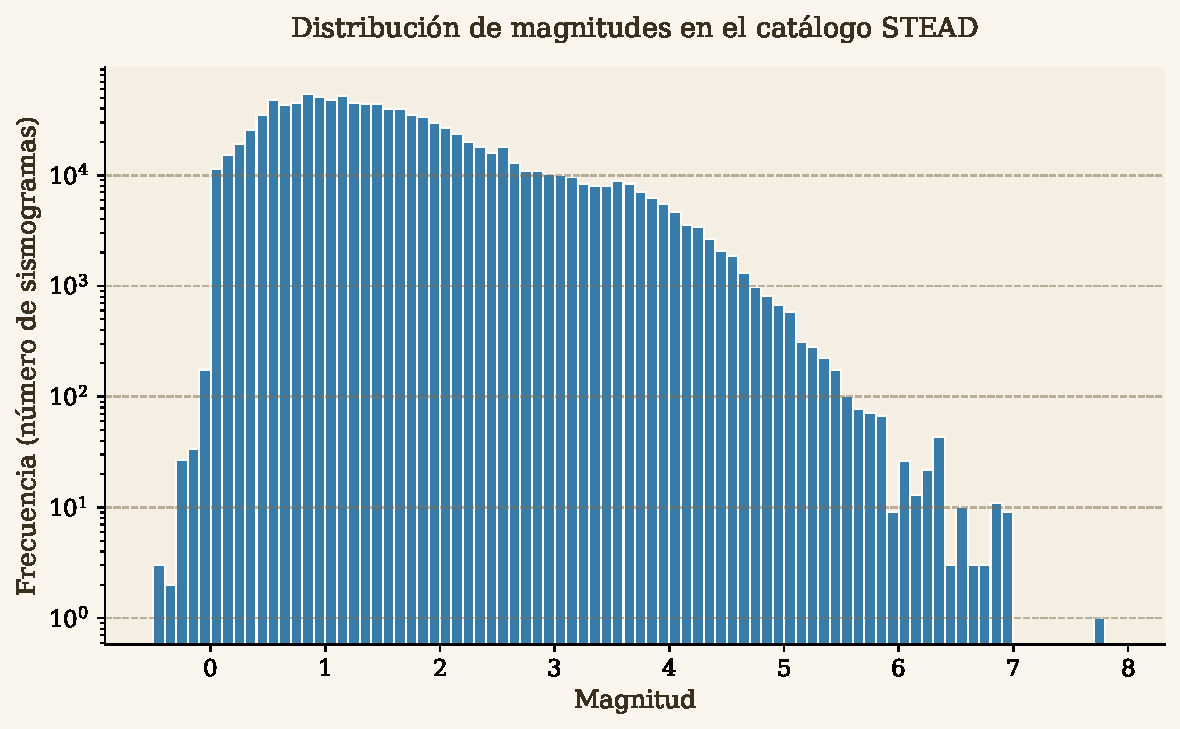
\includegraphics[width=0.85\textwidth]{figuras/figura_histograma_stead}
  \caption[Distribución de magnitudes en el catálogo STEAD]{\textbf{Distribución de magnitudes en el catálogo STEAD.} El histograma muestra la frecuencia de los más de un millón de sismos locales en función de su magnitud (\textbf{nótese la escala logarítmica en el eje Y}). La mayor parte de los eventos registrados se concentran en magnitudes bajas (entre 1 y 3), haciendo visibles también los eventos muy pequeños ($<0.5$) y los escasos grandes terremotos, siguiendo la clásica ley de Gutenberg-Richter.}
  \label{fig:histograma-stead}
\end{figure}

\subsection{Organización del catálogo}
El conjunto de datos se clasifica principalmente en dos tipos de registros:
\begin{itemize}
  \item \textbf{Terremotos locales (\texttt{earthquake\_local}):} Alrededor de $1\,050\,000$ trazas que contienen eventos sísmicos confirmados. En ellas, analistas expertos (o algoritmos de alta fiabilidad) han procedido al picado (\emph{picking}) exacto del instante de llegada de las ondas primarias (P) y secundarias (S).
  \item \textbf{Ruido ambiental (\texttt{noise}):} Unas $450\,000$ trazas correspondientes a periodos de inactividad sísmica. Estas muestras son esenciales como clase negativa para prevenir falsos positivos debidos al ruido generado por la actividad humana o ambiental durante el entrenamiento de modelos de clasificación.
\end{itemize}

\subsection{Los ficheros y sus columnas}
La distribución de STEAD se articula en torno a dos archivos principales, vinculados mediante un identificador único para cada evento:
\begin{enumerate}
  \item Un archivo \texttt{.hdf5} estructurado para almacenar de forma eficiente las matrices multidimensionales correspondientes a las formas de onda crudas.
  \item Un archivo \texttt{.csv} que recoge exhaustivamente los \emph{metadatos}, donde cada fila provee las características analíticas de su sismograma asociado.
\end{enumerate}

Entre los atributos más relevantes incluidos en el archivo tabular, destacan los siguientes:

\begin{itemize}
  \item \textbf{\texttt{trace\_name} y \texttt{trace\_category}:} Constituyen el identificador unívoco del registro y su etiqueta de clase primaria (evento sísmico frente a ruido).
  \item \textbf{\texttt{receiver\_code}, \texttt{receiver\_latitude}, \texttt{receiver\_longitude} y \texttt{receiver\_elevation\_m}:} Proporcionan la identificación y ubicación geoespacial exacta de la estación sismológica receptora.
  \item \textbf{\texttt{source\_magnitude} y \texttt{source\_magnitude\_type}:} Documentan la magnitud del evento y la escala empleada (por ejemplo, magnitud local, $M_L$). Estos campos son exclusivos de los registros clasificados como terremotos.
  \item \textbf{\texttt{source\_latitude}, \texttt{source\_longitude} y \texttt{source\_depth\_km}:} Describen las coordenadas geográficas del epicentro y la profundidad focal de la ruptura (en kilómetros).
  \item \textbf{\texttt{source\_distance\_km} y \texttt{back\_azimuth\_deg}:} Cuantifican la distancia hipocentral y el azimut de propagación, parámetros críticos para caracterizar la atenuación geométrica de las ondas.
  \item \textbf{\texttt{p\_arrival\_sample} y \texttt{s\_arrival\_sample}:} Variables objetivo (\textit{ground truth}) fundamentales para las tareas de regresión temporal; especifican el índice exacto de la muestra discreta ($0$--$5\,999$) correspondiente a los tiempos de llegada de ambas fases.
  \item \textbf{\texttt{p\_status} y \texttt{s\_status}:} Indican la procedencia del picado temporal, distinguiendo entre la intervención de un analista humano (\texttt{manual}) y los sistemas algorítmicos (\texttt{automatic}).
  \item \textbf{\texttt{snr\_db}:} Miden la relación señal-ruido empírica. Valores elevados garantizan una delimitación más nítida de la señal sísmica frente a las perturbaciones de fondo.
\end{itemize}

A partir de este conjunto estructurado, es posible diseñar y entrenar arquitecturas de \textit{Deep Learning} para abordar de manera conjunta la clasificación binaria de la señal (basada en \texttt{trace\_category}) y la regresión precisa de los tiempos de llegada de las fases principales (\texttt{p\_arrival\_sample} y \texttt{s\_arrival\_sample}).

\paragraph{Uso en este TFM.}
En el presente trabajo, se emplean modelos fuertemente consolidados en la literatura, tales como PhaseNet \citep{zhu2018phasenet} y EQTransformer \citep{mousavi2020eqtransformer}, aprovechando su preentrenamiento previo sobre el corpus STEAD mediante la plataforma \emph{SeisBench} \citep{woollam2022seisbench}. Se procede a la validación de sus capacidades predictivas sin requerir un ajuste fino adicional (\textit{zero-shot evaluation}), evaluando su precisión en el picado de fases P y S sobre un subconjunto independiente de eventos y contrastando sus resultados frente a las anotaciones originales del catálogo.

\section{Trabajos relacionados y huecos identificados}
\label{trabajos-relacionados}

La revisión bibliográfica realizada permite identificar el posicionamiento específico de este TFM frente al estado del arte:

\begin{itemize}
  \item \textbf{Frente a ETAS}: el enfoque propuesto retiene la formalización probabilística pero sustituye la forma funcional fija por arquitecturas DL que pueden descubrir patrones no contemplados a priori \citep{ogata1998spacetime, vandenende2024forecasting}.

  \item \textbf{Frente a UCERF3}: UCERF3-ETAS \citep{field2017ucerf3etas} es un modelo operacional consolidado, mientras que el sistema aquí\, propuesto es un prototipo de investigación. No se busca por tanto competir directamente en escala operativa, sino mostrar \emph{si} el DL aporta ganancia metrológicamente significativa sobre los \textit{baselines} clásicos en una región bien caracterizada (California).

  \item \textbf{Frente a PhaseNet/EQTransformer}: estos modelos resuelven el problema \emph{previo} al pronóstico (detección y \textit{picking}). En este TFM se reutilizan como \emph{front-end} preentrenado para alimentar el \emph{back-end} de pronóstico, sin re-entrenarlos.

  \item \textbf{Frente a DeVries et al. (2018) y Rouet-Leduc et al. (2017)}: los trabajos previos más cercanos abordan, respectivamente, la predicción espacial de réplicas y la predicción temporal en laboratorio. Este TFM combina ambas dimensiones (espacial y temporal) sobre catálogos reales con \emph{declustering} explícito para aislar mainshocks independientes.

  \item \textbf{Hueco principal:} la mayoría de los trabajos recientes evaluan un único modelo contra \textit{baselines} débiles, con una sola semilla o sin tests estadísticos. Este TFM aplica en su metodología una comparación exhaustiva y rigurosa \citep{beroza2021dlreview, reichstein2019deep}: multi-semilla, Wilcoxon pareado, multiples \textit{baselines} interpretables, y reproducibilidad estricta.
\end{itemize}

\section{Síntesis}
\label{sintesis}

Las bases teóricas y empíricas revisadas permiten formular tres hipótesis operativas que guiarán la fase experimental:

\begin{enumerate}[label=\textbf{H\arabic*.}]
  \item Las redes preentrenadas \emph{PhaseNet} y \emph{EQTransformer} permiten ejecutar la detección y \textit{picking} de fases P/S sobre STEAD con calidad comparable a la literatura, sin re-entrenamiento.
  \item Una TCN sobre \textit{features} globales del catálogo USGS \emph{no} basta para superar a una regresión logística simple sobre las mismas agregaciones; la señal precursora explotable en estas \textit{features} es de naturaleza estadística, no temporal-secuencial.
  \item La incorporación explícita de la dimensión espacial mediante una GNN sobre celdas activas sí\, mejora significativamente sobre los \textit{baselines}, evidenciando que el cuello de botella del pronóstico sísmico con DL no es la complejidad temporal sino la representación espacial.
\end{enumerate}

% =============================================================================
%                  DESARROLLO DEL PROYECTO Y RESULTADOS
% =============================================================================

\cleardoublepage

\chapter{Desarrollo del proyecto y resultados}
\label{desarrollo-del-proyecto-y-resultados}

Este capítulo describe cómo se ha construido y evaluado el sistema propuesto. Se organiza
en cuatro bloques. El primero (Sección~\ref{metodologia}) detalla la metodología: las
fuentes de datos, las decisiones de diseño, las características, las arquitecturas de los
cinco modelos y, sobre todo, el protocolo de evaluación, que es la pieza que da solidez a
las conclusiones. El segundo (Sección~\ref{planteamiento-del-problema}) formaliza el
problema de pronóstico como una tarea de clasificación y discute sus particularidades. El
tercero (Sección~\ref{desarrollo-del-proyecto}) recorre el desarrollo de las cinco fases
del \textit{pipeline}, una por modelo, indicando las decisiones de implementación. El
cuarto (Sección~\ref{resultados}) presenta los resultados, los compara con los modelos de
referencia y analiza con detalle qué información es capaz de extraer el sistema de los
datos disponibles.

% =============================================================================
\section{Metodología}
\label{metodologia}

La metodología de este trabajo persigue dos objetivos a la vez. Por un lado, la
\emph{validez sismológica} de las decisiones, en línea con la práctica habitual en
geofísica: completitud del catálogo, aislamiento de eventos independientes y elección de
umbrales con justificación física. Por otro lado, la \emph{validez estadística} del
aprendizaje automático: particiones que evitan fugas de información, semillas fijas, varias
repeticiones y comparación sistemática frente a líneas base. Esta doble exigencia recorre
todas las decisiones que se describen a continuación.

\subsection{Esquema general del \textit{pipeline}}
\label{md-pipeline}

El sistema se organiza como una secuencia de cinco fases, cada una con un objetivo propio y
materializada en un \textit{notebook} reproducible. La unidad de análisis cambia entre
fases: en la primera son formas de onda individuales muestreadas a 100\,Hz; en el resto
son días de actividad agregada sobre una región. La Tabla~\ref{tab:pipeline} resume las
cinco fases y la fuente de datos de cada una.

\begin{table}[ht!]
  \centering
  \small
  \begin{tabular}{@{}llll@{}}
    \toprule
    \textbf{Fase} & \textbf{Tarea}                        & \textbf{Modelo}         & \textbf{Datos}     \\
    \midrule
    1             & Detección y \textit{picking} de fases & PhaseNet, EQTransformer & STEAD              \\
    2             & Pronóstico temporal global            & TCN                     & USGS               \\
    3             & Pronóstico espacial                   & GNN (GCN)               & USGS               \\
    4             & Pronóstico espacial con atención      & Transformer geoespacial & USGS               \\
    5             & Mapa de riesgo con incertidumbre      & Proceso Gaussiano       & USGS + Transformer \\
    \bottomrule
  \end{tabular}
  \caption[Estructura del \textit{pipeline} experimental en cinco fases]{\textbf{Estructura del \textit{pipeline} experimental.} Cada fase aborda una tarea distinta, con su propio modelo y su propia fuente de datos. Las dos primeras validan la detección; las tres siguientes abordan el pronóstico y la cartografía del riesgo.}
  \label{tab:pipeline}
\end{table}

El flujo de información es unidireccional. Las dos primeras fases operan sobre trazas sísmicas y validan las herramientas de identificación de eventos; las fases tercera y cuarta
trabajan sobre el catálogo de eventos para anticipar la actividad futura, y la quinta toma
las predicciones del mejor modelo espacial y las transforma en un mapa continuo de riesgo.
Esta separación es deliberada: cada fase responde a una pregunta concreta y puede evaluarse
de forma independiente, lo que facilita aislar qué parte del problema es fácil y qué parte
es difícil.

\subsection{Fuentes de datos y exploración del catálogo}
\label{md-datos}

El trabajo utiliza dos fuentes de datos abiertas y complementarias. Para la fase de
detección se emplea el \textit{STanford EArthquake Dataset} (STEAD), un repositorio de más
de un millón de formas de onda sísmicas etiquetadas con las llegadas de las ondas P y S.
Para las fases de pronóstico se emplea el catálogo del \textit{United States Geological
  Survey} (USGS), descargado a través de su \textit{web service} FDSN. Mientras que STEAD es
ideal para entrenar y validar detectores, el pronóstico necesita un catálogo de eventos
completo y homogéneo en el tiempo, y es ahí donde el USGS resulta insustituible; esta
distinción se justifica de forma empírica en la Sección~\ref{apendice-stead-usgs} del
Apéndice~\ref{apendice-i}.

El catálogo descargado para California y Alaska entre 2000 y 2024 contiene más de 135000
eventos de magnitud \(M \geq 2.5\). La Figura~\ref{fig:eda} resume sus tres dimensiones
fundamentales: la actividad anual, la distribución de magnitudes y la distribución de
profundidades. La actividad anual es relativamente estable, con picos asociados a
secuencias de réplicas de grandes terremotos. La distribución de magnitudes decae de forma
aproximadamente exponencial, como predice la ley de Gutenberg--Richter~\eqref{eq:gr}, lo que
confirma que el catálogo es estadísticamente coherente. La distribución de profundidades
muestra que la mayor parte de la sismicidad ocurre cerca de la superficie, con una cola hacia profundidades
intermedias asociada a la zona de subducción de Alaska.

\begin{figure}[ht!]
  \centering
  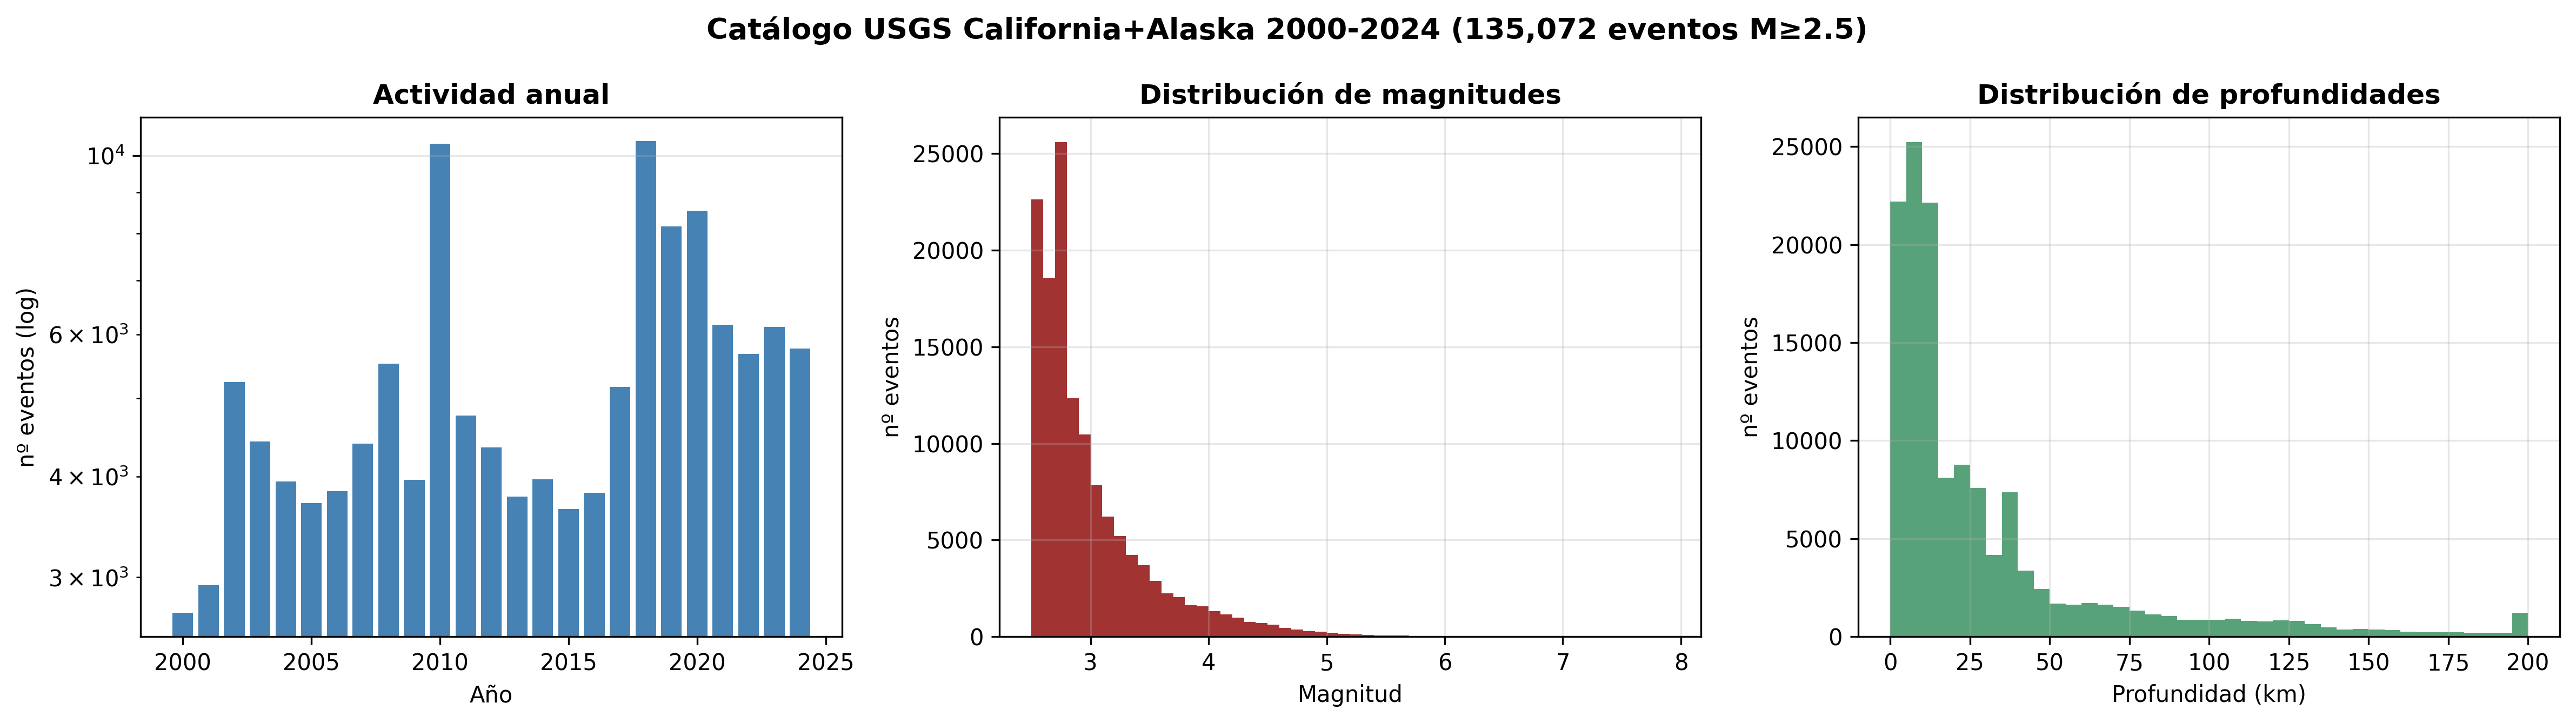
\includegraphics[width=\textwidth]{figuras/03_eda_catalogo}
  \caption[Exploración del catálogo USGS de California y Alaska]{\textbf{Exploración del catálogo USGS (California + Alaska, 2000--2024).} Izquierda: número de eventos por año (escala logarítmica). Centro: distribución de magnitudes. Derecha: distribución de profundidades. El conjunto reúne más de 135.000 eventos de magnitud \(M \geq 2.5\).}
  \label{fig:eda}
\end{figure}

\subsection{Región de estudio y ventana temporal}
\label{md-region}

La región de estudio principal combina dos zonas sísmicamente muy activas y bien
instrumentadas de Estados Unidos: \textbf{California} (\(32^{\circ}\)--\(42^{\circ}\,\)N,
\(-124^{\circ}\)--\(-114^{\circ}\,\)W) y \textbf{Alaska} (\(51^{\circ}\)--\(72^{\circ}\,\)N,
\(-180^{\circ}\)--\(-130^{\circ}\,\)W), en el periodo 2000--2024. La elección responde a
cuatro motivos:

\begin{enumerate}
  \item \textbf{Completitud estable a baja magnitud.} Las redes que cubren ambas zonas
        registran de forma fiable los eventos por encima de \(M_c \approx 2.5\) desde
        mediados de los años noventa. Una magnitud de completitud baja es esencial porque
        las características del modelo se calculan agregando microsismos: si faltaran
        eventos pequeños, esas características estarían sesgadas.
  \item \textbf{Acceso homogéneo.} El catálogo se descarga íntegramente a través del mismo
        \textit{web service}, sin necesidad de combinar fuentes nacionales heterogéneas con
        criterios de catalogación distintos.
  \item \textbf{Más eventos objetivo.} Unir California y Alaska multiplica el número de
        terremotos moderados disponibles para entrenar respecto a usar California sola. Como
        el objetivo del pronóstico son eventos relativamente raros, disponer de más casos
        positivos mejora la robustez estadística del entrenamiento. Conviene matizar este
        punto: aunque California y Alaska responden a regímenes tectónicos distintos, dentro
        de lo que cabe pueden considerarse \emph{compatibles} para entrenar un modelo común.
        Ambas son márgenes muy activos de la placa del Pacífico, con sismicidad
        mayoritariamente somera que sigue la ley de Gutenberg--Richter con \textit{b-values}
        de orden parecido; es decir, las distribuciones estadísticas de sus catálogos --tasas,
        magnitudes, energía-- son lo bastante similares como para que las características
        descritas más adelante tengan el mismo significado en las dos zonas. Esto es lo que
        permite que un mismo modelo aprenda de ambas a la vez sin confundirse.
  \item \textbf{Literatura de referencia abundante.} Ambas regiones están ampliamente
        documentadas, lo que facilita contrastar los valores obtenidos --como el
        \textit{b-value}-- con la literatura y verificar que el preprocesado es correcto.
\end{enumerate}

Conviene señalar que ambas zonas representan regímenes tectónicos distintos: California
está dominada por la falla transformante de San Andrés --donde dos bloques se deslizan
horizontalmente uno respecto al otro-- mientras que Alaska responde a la subducción de la
placa del Pacífico en el arco de las Aleutianas --donde una placa se hunde bajo otra--.
Mantener las dos zonas separadas en el modelado --como se verá en la construcción del grafo
y en la atención del Transformer-- respeta esta diferencia física: el modelo aprende los
patrones \emph{dentro} de cada región sin mezclar geográficamente dos físicas que no tienen
por qué parecerse.

Esta misma observación marca el límite de la estrategia de unir regiones. Podría pensarse en
seguir añadiendo zonas activas --Japón, Chile, el Mediterráneo-- para acumular todavía más
casos positivos, que es el recurso más escaso. Sin embargo, no es aconsejable: cuanto más
heterogéneas son las regiones, más distintas son sus físicas y sus estadísticas, y llega un
punto en que el modelo, que comparte una misma etapa temporal para todas las celdas, ya no
puede aprender una función coherente que sirva para todas a la vez. En otras palabras, el
beneficio de tener más positivos se ve contrarrestado por el ruido de mezclar comportamientos
incompatibles. De hecho, en el desarrollo se probó a ampliar el alcance --incorporando más
fases del catálogo y más regiones-- y el rendimiento no mejoró, lo que confirma de forma
empírica que el equilibrio elegido, dos regiones tectónicamente afines y bien instrumentadas,
es el más adecuado para este trabajo.

\subsection{Magnitud de completitud y declustering}
\label{md-declustering}

Antes de definir el objetivo es necesario tratar dos aspectos del catálogo. El primero es
la \textbf{magnitud de completitud} \(M_c\), el mínimo valor de magnitud a partir del cual
el catálogo se considera completo. En este trabajo se adopta \(M_c = 2.5\), un valor
conservador que asegura completitud incluso en periodos de menor cobertura de la red. Todas
las características se calculan únicamente con eventos por encima de este umbral.

El segundo aspecto, más delicado, es el \textbf{declustering}. Los catálogos sísmicos
contienen secuencias de réplicas que siguen la ley de Omori: tras un terremoto grande
(\textit{mainshock}) llegan numerosos eventos menores cuya tasa decae con el tiempo. Estas
réplicas son altamente predecibles de forma trivial; si no se eliminaran del objetivo,
cualquier modelo aprendería a continuar las secuencias en lugar de a anticipar eventos
nuevos e independientes. Para evitarlo se aplica el algoritmo de Gardner--Knopoff, que para
cada evento candidato a \textit{mainshock} define una ventana espacio-temporal de radio
\(L(M)\)~\eqref{eq:gk-L} y duración \(T(M)\)~\eqref{eq:gk-T} alrededor del evento, y descarta
como dependientes todos los eventos de menor magnitud que caen dentro de ella. El resultado
es un subcatálogo de \emph{mainshocks independientes} sobre el que se define la etiqueta.

Una decisión de diseño central es que el \textit{declustering} se aplica \emph{solo al
  objetivo}, no a las características. El modelo recibe como entrada el catálogo completo
--incluidos los pequeños eventos que podrían contener señal precursora-- y únicamente el
conjunto de mainshocks que define la etiqueta pasa por el filtro. De este modo se purifica
la variable que se quiere predecir sin sacrificar la información de entrada. Esta asimetría
es coherente con la práctica recomendada en la literatura y, como se verá en los estudios
de ablación (Sección~\ref{res-ablations}), resulta metodológicamente necesaria: si no se
declusteriza, el rendimiento aparente sube, pero solo a costa de aprender la
predictibilidad trivial de las réplicas.

\subsection{Definición del objetivo}
\label{md-target}

El objetivo del pronóstico se plantea como un problema binario sobre una ventana de
\textbf{30 días}. En la formulación espacial, para cada celda \(c\) y cada día \(t\) la
etiqueta vale 1 si en los siguientes 30 días ocurre al menos un mainshock independiente de
magnitud \(M \geq 4.5\) relacionado con la celda, y 0 en caso contrario. El umbral
\(M \geq 4.5\) equilibra tres criterios. Primero, un \textbf{volumen suficiente}: por
debajo de \(4.5\) habría demasiados eventos poco relevantes, y por encima de \(5.0\)
quedarían muy pocos casos positivos para entrenar. Segundo, la \textbf{relevancia
  operativa}: un sismo de \(M \geq 4.5\) ya es potencialmente dañino en entornos urbanos
vulnerables. Tercero, la \textbf{homogeneidad del catálogo}: con \(M_c = 2.5\) y un
objetivo en \(4.5\), la distancia de dos unidades de magnitud asegura que el catálogo es
completo tanto para las características como para el objetivo.

En los modelos espaciales, la etiqueta de una celda se calcula además con una
\textbf{expansión 3\(\times\)3}: vale 1 si el mainshock cae en la propia celda o en
cualquiera de sus ocho vecinas inmediatas, lo que equivale a un radio efectivo de unos
55\,km. Esta expansión tiene tres justificaciones. Tiene sentido físico --interesa saber si
habrá un terremoto \emph{cerca}, no en una celda exacta--; absorbe el error de localización
del catálogo, que es de varios kilómetros; y evita que la proporción de positivos por celda
baje a niveles que impidan el aprendizaje. Aun con la expansión, el problema es fuertemente
desbalanceado, como se discute en la Sección~\ref{planteamiento-del-problema}.

\subsection{Ingeniería de características}
\label{md-features}

Antes de calcular las características se discretiza la región en una rejilla regular de
celdas de \(0.5^{\circ} \times 0.5^{\circ}\), aproximadamente 50\,km de lado. Cada
evento se asigna a la celda que lo contiene. Se conservan únicamente las \emph{celdas
  activas}, definidas como aquellas con al menos 30 eventos en todo el periodo; las celdas con
muy poca actividad aportan más ruido que señal y se descartan para evitar la maldición de la
dimensionalidad. La Figura~\ref{fig:grid} muestra la rejilla resultante: la sismicidad se
concentra claramente a lo largo de las grandes estructuras tectónicas.

\begin{figure}[ht!]
  \centering
  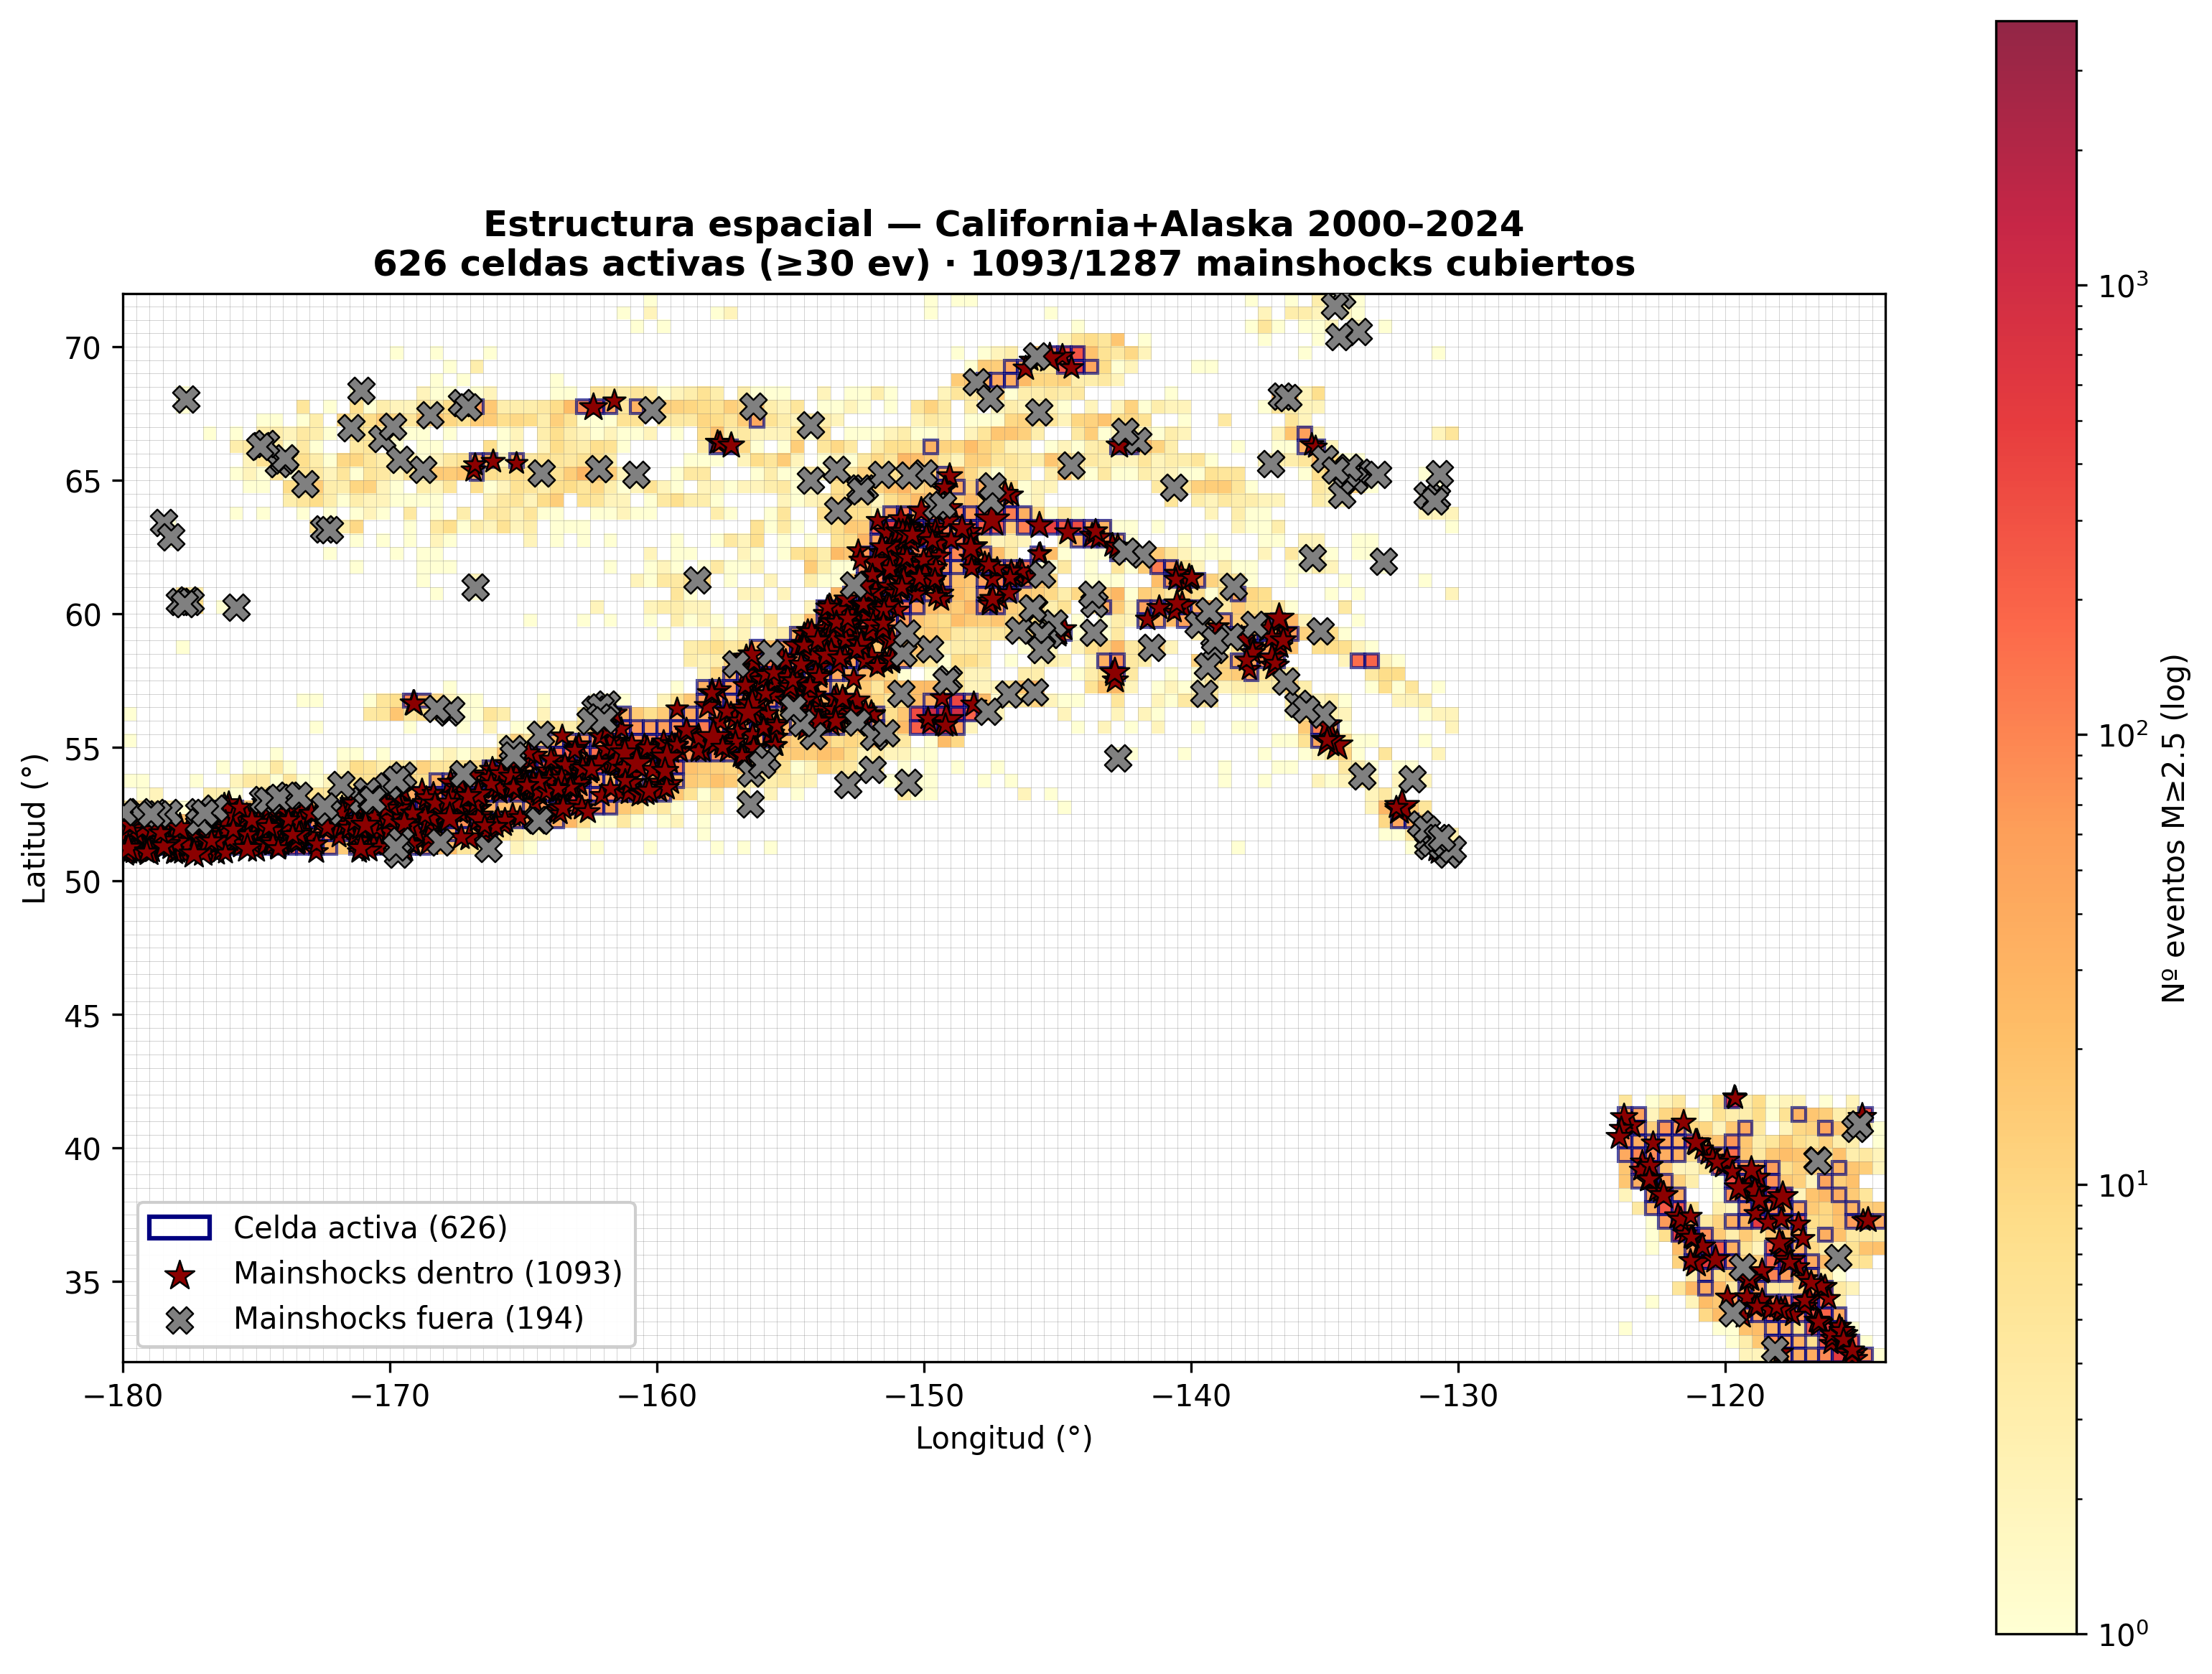
\includegraphics[width=0.92\textwidth]{figuras/05_grid_espacial_M4.5_min30}
  \caption[Discretización espacial en celdas y celdas activas]{\textbf{Discretización espacial de la región de estudio.} Cada evento se asigna a una celda de \(0.5^{\circ}\times 0.5^{\circ}\); se conservan las celdas con al menos 30 eventos (celdas activas). La sismicidad se alinea con la falla de San Andrés en California y con el arco de las Aleutianas en Alaska.}
  \label{fig:grid}
\end{figure}

Para cada celda activa y cada día se calculan cinco características, pensadas para capturar
distintos aspectos de la actividad sísmica:

\begin{enumerate}
  \item \textbf{Recuento logarítmico} de eventos del día, \(\log(1+n)\), donde \(n\) es el
        número de eventos con \(M \geq M_c\). La transformación logarítmica comprime el
        rango dinámico, ya que un evento grande puede generar miles de réplicas en un solo
        día y desestabilizaría el entrenamiento sin esta compresión.
  \item \textbf{Energía logarítmica} liberada, \(\log(1+E)\), donde la energía \(E\) se
        obtiene de la magnitud mediante la relación~\eqref{eq:kanamori}. Esta característica
        pondera los eventos por su tamaño y no solo por su número.
  \item \textbf{Magnitud máxima} registrada en la celda ese día, que destaca la presencia de
        eventos moderados.
  \item \textbf{Recuento de eventos moderados} (\(M \geq 3.5\)) en escala logarítmica, que
        aísla la actividad más energética del ruido de microsismos.
  \item \textbf{\textit{b-value} móvil} de 30 días, estimado por máxima verosimilitud con el
        estimador de Aki~\eqref{eq:b-aki}. El \textit{b-value} resume la proporción entre
        sismos pequeños y grandes y tiene significado físico: descensos transitorios se
        asocian a un mayor estado de estrés. Se calcula por región y no por celda, porque su
        estimación necesita decenas de eventos para ser estable, y se asigna a cada celda el
        valor de su región.
\end{enumerate}

Otras características también se probaron en varios experimentos sin que mejoraran el modelo,
por lo que finalmente se descartaron y no forman parte del conjunto definitivo. La primera fue
la \textbf{profundidad} de los terremotos: se añadió un sexto canal con la profundidad media de
los seísmos de cada celda y día --en una variante, ponderada por la energía de los eventos, de
modo que un terremoto grande y profundo pesara más que un microsismo somero--, con la idea de
que la profundidad ayuda a distinguir regímenes sísmicos distintos, como los eventos profundos
de la subducción de Alaska frente a los corticales someros. Sin embargo, la profundidad media
diaria resultó muy volátil y, lejos de ayudar, redujo ligeramente el rendimiento; una posible
explicación es que su información ya está parcialmente recogida de forma implícita por la
energía. La segunda familia de características ensayada fueron \textbf{indicadores de anomalía
  de la tasa sísmica} por celda --que comparan la actividad reciente en una ventana corta con su
línea base en una ventana larga-- pensados para captar aceleraciones o silencios sísmicos que
la literatura asocia a posibles precursores; tampoco aportaron señal apreciable. En total se
llegó a tantear hasta ocho canales, pero ninguna de estas adiciones superó a las cinco
características originales.

La Tabla~\ref{tab:features} resume las cinco características, su transformación y la dimensión
del fenómeno que cada una pretende capturar. En conjunto cubren tres aspectos complementarios
de la sismicidad: \emph{cuánta} actividad hay (recuentos), \emph{cómo de energética} es
(energía y magnitud máxima) y \emph{cómo se reparte} entre tamaños (\textit{b-value}). Esta
diversidad busca dar al modelo una visión completa del estado de cada celda con un número
reducido de variables, lo que es deseable dado el tamaño limitado del conjunto de datos.

\begin{table}[ht!]
  \centering
  \small
  \begin{tabular}{@{}llll@{}}
    \toprule
    \textbf{\#} & \textbf{Característica}  & \textbf{Transformación} & \textbf{Captura}     \\
    \midrule
    1           & Recuento de eventos      & $\log(1+n)$             & volumen de actividad \\
    2           & Energía liberada         & $\log(1+E)$             & energía total        \\
    3           & Magnitud máxima          & valor directo           & eventos destacados   \\
    4           & Recuento $M\geq 3.5$     & $\log(1+n_{3.5})$       & actividad energética \\
    5           & \textit{b-value} (30\,d) & estimador de Aki        & reparto por tamaños  \\
    \bottomrule
  \end{tabular}
  \caption[Características de entrada de los modelos de pronóstico]{\textbf{Características de entrada.} Las cinco variables calculadas por celda y día, con su transformación y el aspecto de la sismicidad que capturan. Todas se calculan de forma causal sobre eventos $M\geq M_c$.}
  \label{tab:features}
\end{table}

Dos cuidados son esenciales para la validez del experimento. Primero, todas las
características se calculan de forma \emph{causal}: cada valor en el día \(t\) usa únicamente
información hasta ese día, de modo que en ningún momento entra información del futuro.
Segundo, la normalización a media cero y desviación uno se ajusta exclusivamente sobre el
conjunto de entrenamiento, y las mismas medias y desviaciones se aplican después a
validación y test, evitando así cualquier fuga de información entre particiones.

El Algoritmo~\ref{alg:dataset} resume el procedimiento completo de construcción del conjunto
de datos espacio-temporal, desde el catálogo bruto hasta los tensores de entrada y las
etiquetas que reciben los modelos. Su lectura permite verificar, paso a paso, que la
causalidad y la separación entre características y objetivo se respetan en todo momento.

\begin{algorithm}[ht!]
  \caption{Construcción del conjunto de datos espacio-temporal}
  \label{alg:dataset}
  \DontPrintSemicolon
  \KwIn{Catálogo de eventos $\mathcal{C}$; magnitud de completitud $M_c$; umbral objetivo $M_t=4.5$; ventana de historia $L=60$; ventana de predicción $T=30$.}
  \KwOut{Tensor de características $X$, matriz de etiquetas $Y$, grafo $G$.}
  Discretizar la región en celdas de $0.5^{\circ}\times 0.5^{\circ}$ y asignar cada evento a su celda\;
  Conservar las celdas con $\geq 30$ eventos (celdas activas)\;
  Construir el grafo $G$ uniendo celdas a $<100$\,km dentro de cada región\;
  Obtener el subcatálogo de mainshocks independientes con Gardner--Knopoff\;
  \For{cada celda activa $c$}{
    \For{cada día $t$}{
      Calcular las 5 características causales con eventos $M\geq M_c$ hasta $t$\;
      $Y[c,t] \leftarrow 1$ si hay un mainshock $M\geq M_t$ en $c$ o sus vecinas en $[t+1,t+T]$; si no, $0$\;
    }
  }
  Particionar en train (2000--2020), validación (2021--2022) y test (2023--2024)\;
  Ajustar la normalización en train y aplicarla a las tres particiones\;
  \Return $X$, $Y$, $G$\;
\end{algorithm}

\subsection{Construcción del grafo espacial}
\label{md-grafo}

Los modelos espaciales necesitan una noción de vecindad entre celdas. Esta se representa
como un grafo \(G=(V,E)\) en el que cada celda activa es un nodo y existe una arista entre
dos celdas si su distancia, medida con la fórmula de Haversine~\eqref{eq:haversine}, es
menor que 100\,km. Para garantizar que ninguna celda quede aislada --lo que dejaría sus
características estancadas en la propagación-- se añade además una conexión a las dos vecinas
más cercanas aunque superen el umbral. Como California y Alaska están separadas por más de
3.000\,km, las aristas se restringen al interior de cada región: el grafo final tiene dos
componentes conexas, una por zona, y el modelo opera sobre ambas a la vez. La
Figura~\ref{fig:grafo} muestra el grafo sobre el mapa.

\begin{figure}[ht!]
  \centering
  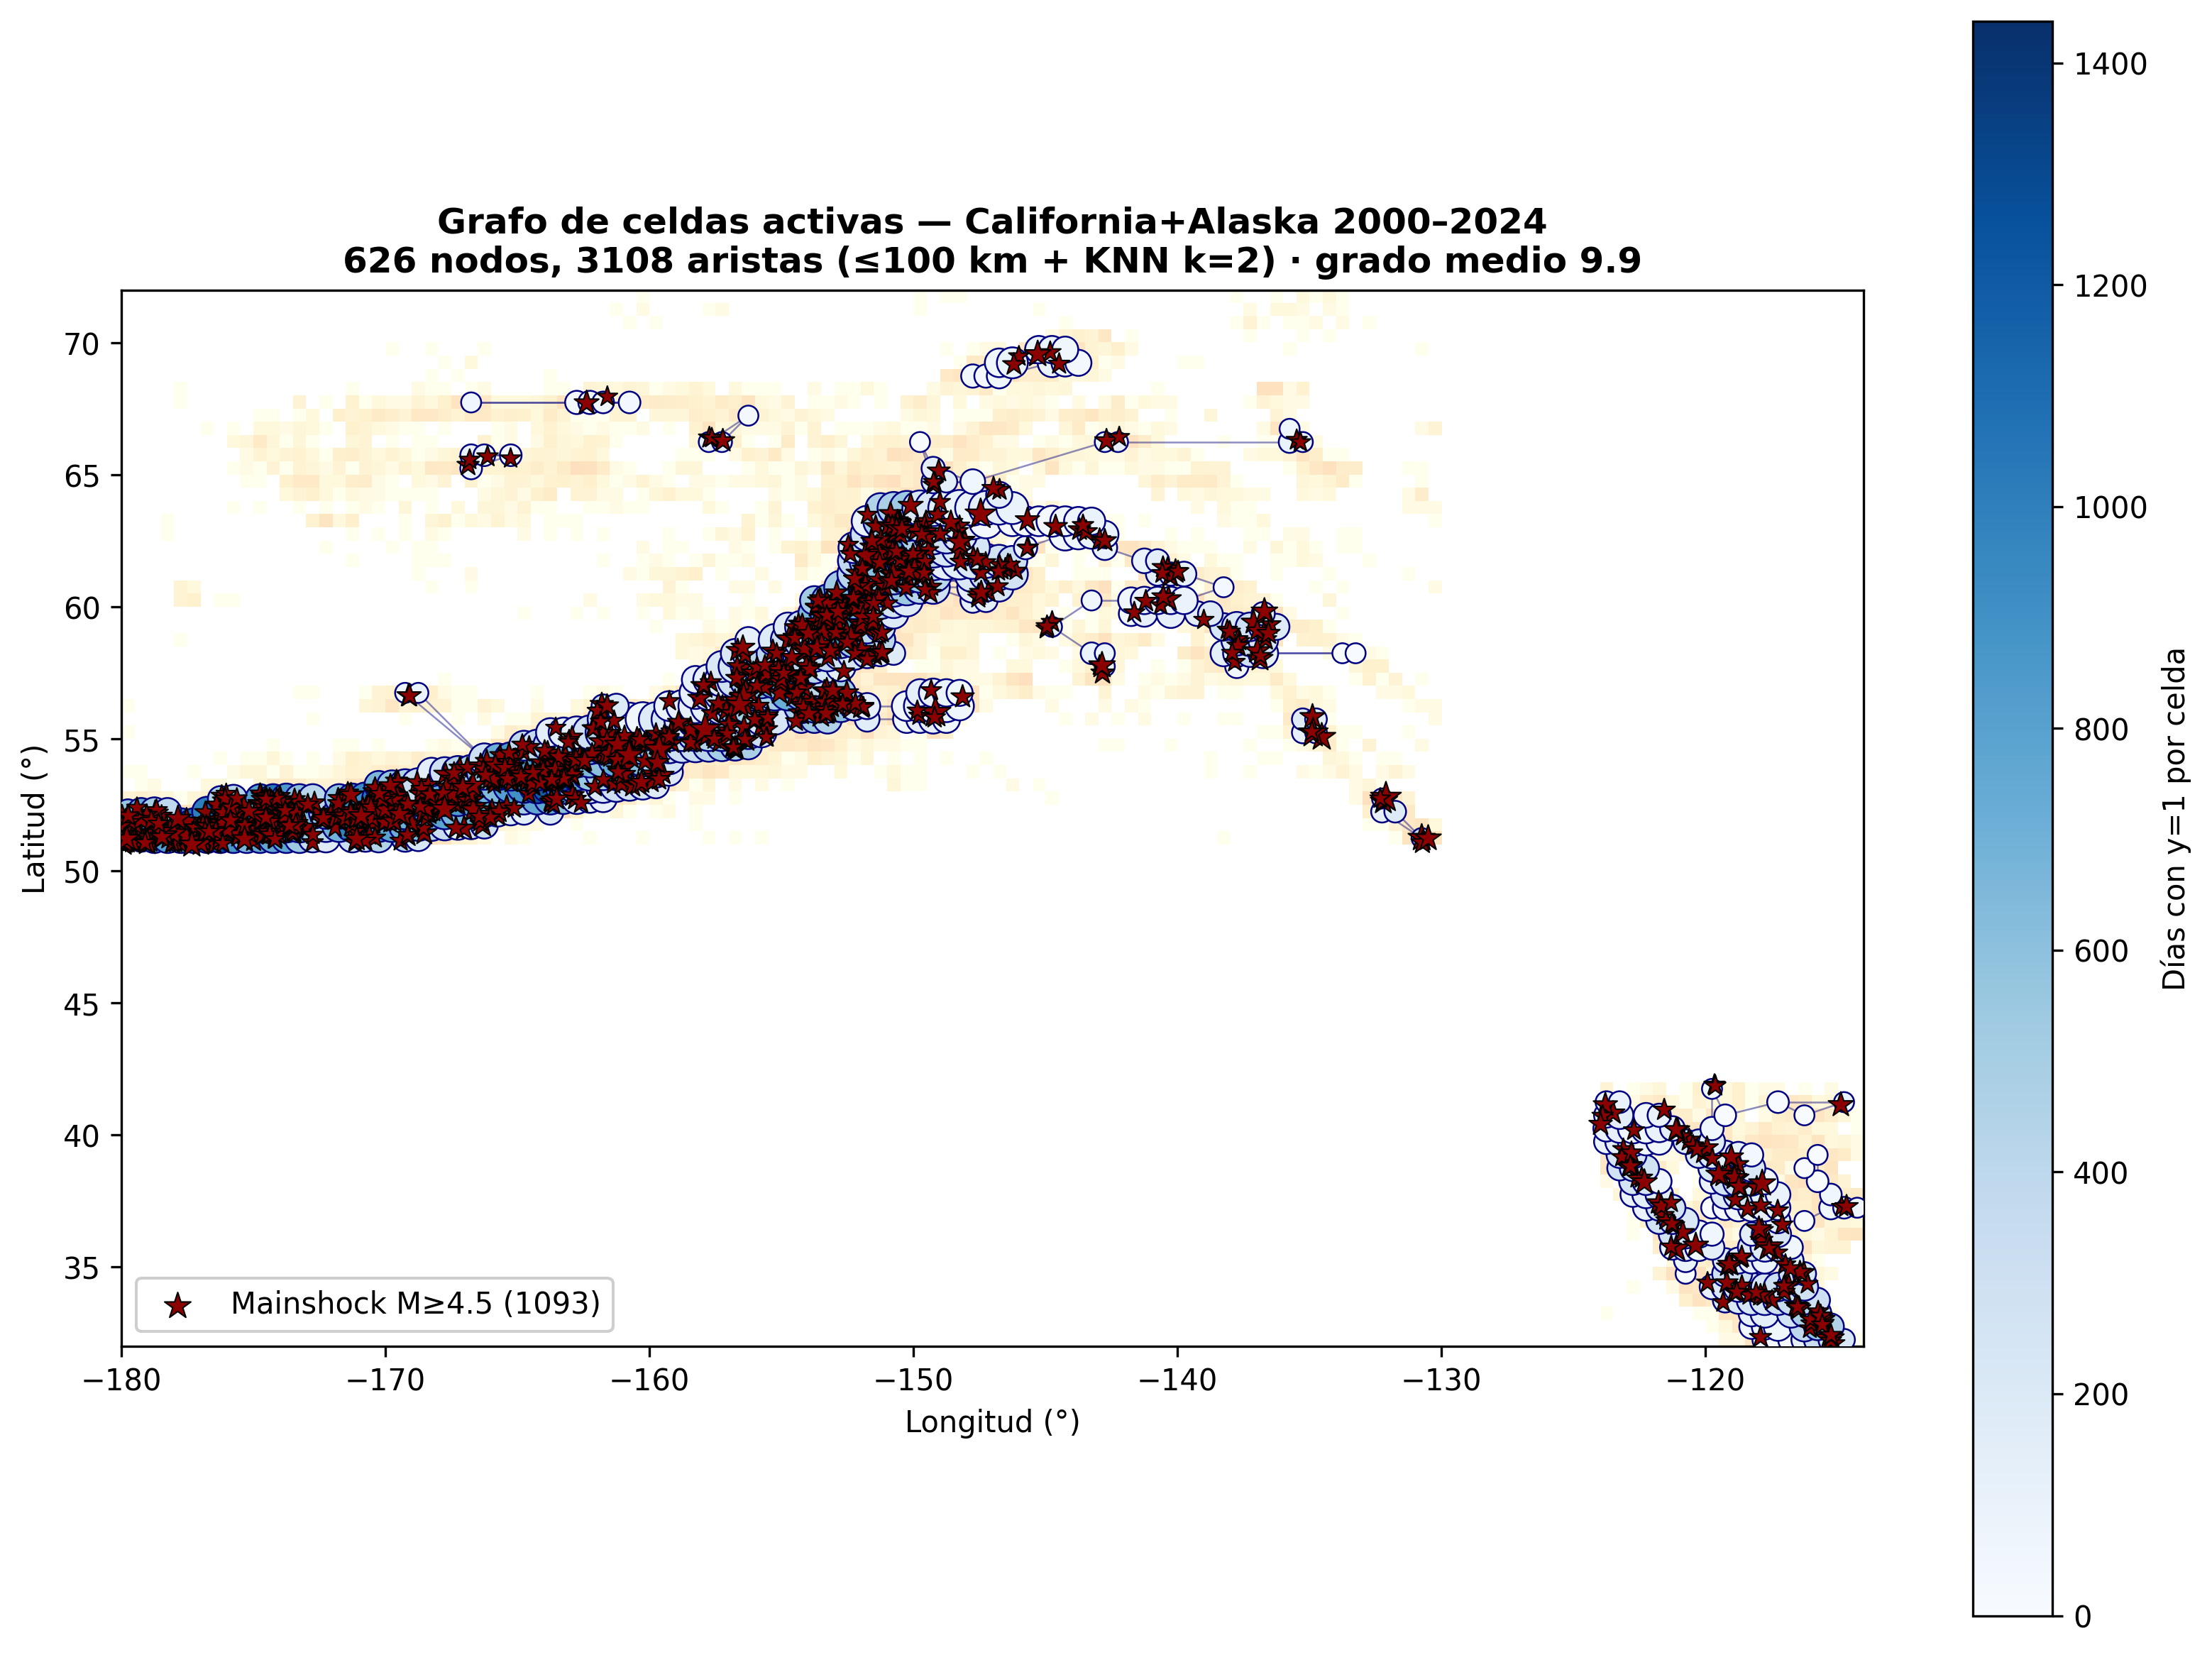
\includegraphics[width=0.92\textwidth]{figuras/05_grafo_celdas_d100km}
  \caption[Grafo de vecindad entre celdas activas]{\textbf{Grafo de vecindad espacial.} Los nodos son las celdas activas y las aristas conectan celdas a menos de 100\,km dentro de la misma región. La estructura reproduce los grandes alineamientos tectónicos y mantiene separadas las dos zonas de estudio.}
  \label{fig:grafo}
\end{figure}

\subsection{Particiones temporales}
\label{md-splits}

Para evitar que el modelo ``vea el futuro'' durante el entrenamiento, las particiones son
estrictamente temporales, no aleatorias. El conjunto de \textbf{entrenamiento} abarca de
2000 a 2020, el de \textbf{validación} 2021--2022 --usado para la parada temprana y la
selección de hiperparámetros-- y el de \textbf{test} 2023--2024, reservado por completo para
la evaluación final. Este esquema reproduce las condiciones reales de un sistema de
pronóstico: en cada instante solo se dispone del pasado. Conviene notar que el historial de
60 días que mira el modelo para predecir el primer día de test procede del final del periodo
de validación; esto no constituye fuga de información, ya que se trata de datos de entrada
(el pasado observable) y nunca de las etiquetas de test, que permanecen intactas durante todo
el desarrollo.

\subsection{Arquitecturas de los modelos}
\label{md-arquitecturas}

Esta sección describe en detalle las cuatro arquitecturas que componen el \textit{pipeline}
de pronóstico y cartografía. Todas comparten un mismo bloque temporal --una red convolucional
temporal-- y se diferencian en cómo tratan la dimensión espacial.

\subsubsection{Red convolucional temporal (TCN)}
\label{md-arq-tcn}

La TCN es el bloque que procesa la evolución temporal de las características. Sustituye la
recurrencia de las redes recurrentes clásicas por una pila de convoluciones unidimensionales
con tres propiedades. Son \emph{causales}, es decir, la salida en el instante \(t\) depende
solo de las entradas en instantes \(t' \leq t\), lo que se logra desplazando la convolución
para no usar el futuro. Son \emph{dilatadas}: la capa \(\ell\)-ésima usa una dilatación
\(d_\ell = 2^{\ell-1}\), de modo que el campo receptivo crece exponencialmente con la
profundidad según la relación~\eqref{eq:rf-tcn}. Y emplean \emph{bloques residuales}, en los
que cada bloque suma su entrada a su salida, lo que facilita el entrenamiento de redes
profundas.

Cada \textbf{bloque residual} contiene dos convoluciones causales dilatadas, cada una seguida
de una normalización, una función de activación no lineal y una capa de \textit{dropout}; la
entrada del bloque se suma a su salida mediante una conexión de atajo (cuando las dimensiones
no coinciden, la conexión incluye una convolución \(1\times 1\) que las ajusta). Esta suma
residual es la que permite que el gradiente fluya sin atenuarse a través de muchas capas, de
modo que la red profunda se entrena con estabilidad. Formalmente, si \(\mathbf{x}\) es la
entrada del bloque y \(\mathcal{F}\) la transformación de sus dos convoluciones, la salida es
\(\mathbf{y} = \text{act}(\mathbf{x} + \mathcal{F}(\mathbf{x}))\).

En la configuración utilizada, la pila tiene tres niveles con dilataciones \(\{1,2,4\}\) y
canales \((32, 32, 64)\), o cuatro niveles con dilataciones \(\{1,2,4,8\}\) en la variante
global del notebook de pronóstico temporal. El tamaño de \textit{kernel} es \(k=3\). Aplicando
la relación~\eqref{eq:rf-tcn}, el campo receptivo de la variante de cuatro niveles abarca
\(1 + 2\,(k-1)\sum_{\ell} d_\ell = 1 + 2\cdot 2\cdot(1{+}2{+}4{+}8) = 61\) días, justo lo
necesario para cubrir la ventana de historia de 60 días sin desperdiciar capacidad. Esta es la
ventaja esencial de las dilataciones: alcanzar un horizonte temporal amplio con muy pocas capas
y, por tanto, con pocos parámetros.

La cabeza de clasificación no se limita al último instante temporal, sino que concatena tres
estadísticos de la secuencia de salida: el estado final causal, la media y el máximo a lo largo
del tiempo. Esto da al modelo acceso explícito tanto al ``presente'' (el último día) como a
estadísticos globales de toda la ventana, lo que mejora la sensibilidad a patrones distribuidos
en el tiempo, como un aumento sostenido de la actividad. En el modelo temporal global, la salida
es un único logit; en los modelos espaciales, la TCN se aplica de forma compartida a cada celda,
produciendo un vector de características por celda que alimenta la etapa espacial.

El Algoritmo~\ref{alg:tcn} resume el paso hacia delante de la TCN, desde la ventana de historia
hasta la representación que usa la cabeza de clasificación. Es el bloque base del sistema: en la
Fase 2 produce directamente un \textit{logit}, y en las Fases 3 y 4 se reutiliza, con los mismos
pesos, para resumir la historia de cada celda antes de la etapa espacial.

\begin{algorithm}[ht!]
  \caption{Paso hacia delante de la red convolucional temporal (TCN)}
  \label{alg:tcn}
  \DontPrintSemicolon
  \KwIn{Serie de características $X \in \mathbb{R}^{L\times F}$ (ventana de $L=60$ días, $F=5$ características); dilataciones $\{d_1,\dots,d_B\}=\{1,2,4,8\}$.}
  \KwOut{\textit{Logit} de riesgo (Fase 2) o vector de características (Fases 3--4).}
  $h \leftarrow X$\;
  \For{cada bloque residual $b = 1,\dots,B$}{
    $z \leftarrow \text{ConvCausalDilatada}_{d_b}(h)$ \tcp*{2 convoluciones, \textit{kernel} 3}
    $z \leftarrow \text{Dropout}(\text{act}(\text{Norm}(z)))$\;
    $h \leftarrow \text{act}\big(h + z\big)$ \tcp*{suma residual (atajo $1{\times}1$ si hace falta)}
  }
  $e \leftarrow [\,h^{\text{final}} \,\|\, \overline{h} \,\|\, \max h\,]$ \tcp*{\textit{pooling} temporal}
  \eIf{modelo temporal global (Fase 2)}{
    \Return $w^\top e + b$ \tcp*{un único \textit{logit}}
  }{
    \Return $e$ \tcp*{vector de características de la celda}
  }
\end{algorithm}

\subsubsection{Red neuronal de grafos (GNN)}
\label{md-arq-gnn}

La GNN es el primer modelo que incorpora la dimensión espacial. Su arquitectura,
denominada \textit{SpatioTemporalGNN}, combina dos bloques. En primer lugar, una \textbf{TCN
  compartida} procesa la serie temporal de cada celda de forma independiente, con los mismos
pesos para todas las celdas (\textit{weight sharing}); el resultado es un vector de
características o \textit{embedding} por celda, que resume su historia reciente. En segundo
lugar, \textbf{dos capas convolucionales de grafo} (GCN) propagan información entre celdas
vecinas.

Cada capa GCN aplica la operación~\eqref{eq:gcn}, que en su forma matricial se escribe
\(H^{(l+1)} = \sigma\!\big(\tilde{D}^{-1/2}\tilde{A}\,\tilde{D}^{-1/2} H^{(l)} W^{(l)}\big)\),
donde \(\tilde{A} = A + I\) es la matriz de adyacencia con bucles propios añadidos --para que
cada celda tenga en cuenta también su propia información--, \(\tilde{D}\) es su matriz de
grados y \(W^{(l)}\) es la matriz de pesos aprendible de la capa. La normalización simétrica
\(\tilde{D}^{-1/2}\tilde{A}\,\tilde{D}^{-1/2}\) evita que las celdas con muchos vecinos
dominen la propagación, equilibrando la contribución de cada nodo. Intuitivamente, cada capa
sustituye el vector de una celda por una media ponderada de los vectores de sus vecinas (y el
suyo propio), seguida de una transformación lineal y una no linealidad. Apilando dos capas,
cada celda recibe información de su entorno a dos saltos de distancia. Una cabeza lineal por
nodo produce finalmente un logit por celda.

El uso de pesos compartidos en la TCN y de matrices de adyacencia precomputadas mantiene el
número de parámetros moderado, en torno a las decenas de miles, lo que es adecuado para un
conjunto de datos de tamaño limitado. Es importante subrayar que el modelo no memoriza celdas
concretas: aprende una \emph{función} de las características y de la estructura de vecindad,
lo que en principio permitiría aplicarlo a otras regiones sin reentrenar desde cero.

\subsubsection{Transformer geoespacial}
\label{md-arq-transformer}

El Transformer geoespacial explora una segunda forma de modelar el espacio. Mantiene el mismo
procesamiento temporal por celda mediante una TCN compartida, pero sustituye la propagación
por grafo por un mecanismo de \textbf{atención}. En lugar de imponer de antemano qué celdas
son vecinas, la atención~\eqref{eq:attention} permite que el modelo aprenda, para cada
predicción, qué celdas son relevantes, ponderando la contribución de cada una.

El mecanismo funciona del siguiente modo. El \textit{embedding} de cada celda se proyecta en
tres vectores: una \emph{consulta} (\textit{query}), una \emph{clave} (\textit{key}) y un
\emph{valor} (\textit{value}). La relevancia de la celda \(j\) para la celda \(i\) se calcula
como el producto escalar entre la consulta de \(i\) y la clave de \(j\), escalado por la raíz
de la dimensión y normalizado con una función \textit{softmax} sobre todas las celdas; el
nuevo vector de la celda \(i\) es entonces la media de los valores, ponderada por esas
relevancias. Este cómputo se realiza en paralelo en \textbf{cuatro cabezas} de atención, cada
una con sus propias proyecciones, lo que permite al modelo atender simultáneamente a distintos
tipos de relación espacial; las salidas de las cuatro cabezas se concatenan y se combinan. La
posición geográfica de cada celda se inyecta mediante una \textbf{codificación posicional
  sinusoidal} de sus coordenadas, análoga a la usada en el procesamiento de lenguaje pero
adaptada a coordenadas continuas: la mitad de las dimensiones codifican la latitud y la otra
mitad la longitud, mediante senos y cosenos a frecuencias geométricamente espaciadas, de modo
que celdas próximas reciben codificaciones parecidas y el modelo puede inferir distancias.

La configuración emplea una dimensión de \textit{embedding} de 128, cuatro cabezas de
atención y dos capas de codificador, cada una con su bloque de atención y su red
\textit{feed-forward}, conectadas por sumas residuales y normalización. Para respetar la
separación tectónica entre California y Alaska, la atención se restringe mediante una máscara
que asigna relevancia nula (un valor \(-\infty\) antes de la \textit{softmax}) a los pares de
celdas de regiones distintas: cada celda solo presta atención a las de su propia región. Esta
variante enmascarada es la que mejor rendimiento ofrece y la que alimenta la fase de
cartografía. Una cabeza lineal por celda produce el logit final.

Pese a sus diferencias, la GNN y el Transformer comparten el mismo esqueleto de cómputo, que
el Algoritmo~\ref{alg:forward} hace explícito: una etapa temporal idéntica, compartida entre
todas las celdas, seguida de una etapa de mezcla espacial que es lo único que distingue a
ambos modelos. Esta estructura común es precisamente lo que permite atribuir las diferencias
de rendimiento al mecanismo espacial y no al procesamiento temporal.

\begin{algorithm}[ht!]
  \caption{Paso hacia delante de los modelos espaciales (GNN / Transformer)}
  \label{alg:forward}
  \DontPrintSemicolon
  \KwIn{Ventana de características $X \in \mathbb{R}^{N\times L\times 5}$ ($N$ celdas, $L$ días); grafo $G$ (GNN) o coordenadas $(\text{lat},\text{lon})$ (Transformer).}
  \KwOut{Logits de riesgo $z \in \mathbb{R}^{N}$ (uno por celda).}
  \For{cada celda $c \in \{1,\dots,N\}$}{
    $e_c \leftarrow \text{TCN}_\theta(X_c)$ \tcp*{Algoritmo~\ref{alg:tcn}, misma $\theta$ para todas las celdas}
  }
  $E \leftarrow [e_1,\dots,e_N]$ \tcp*{matriz de \textit{embeddings} de celda}
  \eIf{modelo $=$ GNN}{
    \For{cada capa $\ell = 1, 2$}{
      $E \leftarrow \sigma\big(\tilde{D}^{-1/2}\tilde{A}\,\tilde{D}^{-1/2}\, E\, W^{(\ell)}\big)$ \tcp*{GCN: media sobre vecinos del grafo}
    }
  }{
    $E \leftarrow E + \text{PosEnc}(\text{lat},\text{lon})$ \tcp*{codificación geográfica}
    \For{cada capa $\ell = 1, 2$}{
      $E \leftarrow \text{AtenciónMultiCabeza}_{\text{enmasc.}}(E)$ \tcp*{cada celda atiende a las de su región}
    }
  }
  \For{cada celda $c$}{ $z_c \leftarrow w^\top E_c + b$ \tcp*{cabeza lineal por celda} }
  \Return $z$\;
\end{algorithm}

\subsubsection{Proceso Gaussiano para la cartografía del riesgo}
\label{md-arq-gp}

La última arquitectura no es una red neuronal, sino un \textbf{proceso gaussiano} (GP), un
método bayesiano no paramétrico ideal para interpolar con incertidumbre. Un GP define una
distribución de probabilidad sobre funciones, caracterizada por una función de media y una
función de covarianza o \textit{kernel} \(k(\mathbf{x},\mathbf{x}')\), que codifica cómo de
parecidos se espera que sean los valores de la función en dos puntos según su distancia. Dadas
unas observaciones --en este caso, las probabilidades de riesgo calibradas en los centroides de
las celdas activas-- el GP produce, para cualquier punto \(\mathbf{x}_*\) del mapa, una
predicción que es a su vez una distribución gaussiana. Su media es
\(\mu_* = \mathbf{k}_*^\top (K + \sigma^2 I)^{-1}\mathbf{y}\) --una media ponderada de las
observaciones, donde el peso de cada una decae con la distancia-- y su varianza es
\(\sigma_*^2 = k(\mathbf{x}_*,\mathbf{x}_*) - \mathbf{k}_*^\top (K + \sigma^2 I)^{-1}\mathbf{k}_*\),
que crece a medida que el punto se aleja de las observaciones. De ahí que el GP entregue de
forma natural, y sin coste adicional, el mapa de incertidumbre junto al de riesgo.

Se emplea un \textit{kernel} de tipo Matérn, habitual en datos espaciales porque genera
superficies suaves pero no excesivamente regulares, más realistas para un fenómeno físico que el
\textit{kernel} gaussiano. El parámetro de suavidad \(\nu\) del Matérn controla cuántas veces es
diferenciable la superficie resultante; valores intermedios (como \(\nu = 3/2\)) producen mapas
con un grado de rugosidad coherente con la distribución real de la sismicidad. Los parámetros del
\textit{kernel} --la escala de longitud y la varianza-- se ajustan por máxima verosimilitud sobre
las propias observaciones. El GP se ajusta por separado en cada región, ya que interpolar a
través de los 3.000\,km que separan California y Alaska no tendría ningún sentido físico.

\subsection{Función de pérdida y manejo del desbalance}
\label{md-loss}

El pronóstico sísmico es un problema fuertemente desbalanceado: en la formulación por celda,
solo en torno al 4.5\,\% de los pares (celda, día) son positivos. Si no se corrige, un
modelo entrenado con la entropía cruzada habitual tendería a predecir siempre ``no habrá
terremoto'', que es correcto la mayor parte del tiempo pero inútil. Para evitarlo se utiliza
una entropía cruzada binaria con \emph{ponderación de clase}, que asigna a los ejemplos
positivos un peso proporcional a su escasez, de modo que el modelo no pueda ignorarlos. En
algunas variantes se emplea además una \emph{pérdida focal}, que reduce automáticamente el
peso de los ejemplos fáciles de clasificar y concentra el aprendizaje en los difíciles. Estas
elecciones permiten que el entrenamiento atienda a la clase minoritaria sin necesidad de
sobremuestrearla.

\subsection{Optimización, entrenamiento y reproducibilidad}
\label{md-optim}

Todos los modelos se entrenan con el optimizador Adam, con una tasa de aprendizaje inicial
del orden de \(10^{-4}\)--\(10^{-3}\), regularización \(L_2\) sobre los pesos y
\textit{dropout} para evitar el sobreajuste, especialmente importante dado el tamaño limitado
del conjunto de datos. Se emplea además un planificador que reduce la tasa de aprendizaje
cuando la métrica de validación deja de mejorar, y una parada temprana que detiene el
entrenamiento y recupera el mejor punto cuando la validación no progresa durante un número
fijo de épocas. La Tabla~\ref{tab:hiperparametros} reúne los hiperparámetros más relevantes
del sistema; el detalle completo, separado en hiperparámetros de \emph{arquitectura} y de
\emph{entrenamiento} para cada uno de los tres modelos, se recoge en las
Tablas~\ref{tab:hiper-arq} y~\ref{tab:hiper-train} del Apéndice~\ref{apendice-i}.

\begin{table}[ht!]
  \centering
  \small
  \begin{tabular}{@{}ll@{}}
    \toprule
    \textbf{Hiperparámetro}                 & \textbf{Valor}                               \\
    \midrule
    Ventana de historia (\textit{lookback}) & 60 días                                      \\
    Ventana de predicción                   & 14 días (TCN) / 30 días (modelos espaciales) \\
    Tamaño de \textit{kernel} de la TCN     & 3                                            \\
    Dim.\ de mezcla espacial                & 64 (GNN, GCN) / 128 (Transformer, atención)  \\
    Optimizador                             & Adam                                         \\
    Tasa de aprendizaje                     & $10^{-4}$--$10^{-3}$                         \\
    \textit{Dropout}                        & 0.15--0.20                                   \\
    Parada temprana                         & sí (paciencia 6--12 épocas)                  \\
    \bottomrule
  \end{tabular}
  \caption[Hiperparámetros más relevantes del sistema]{\textbf{Hiperparámetros más relevantes} del sistema. El detalle completo por modelo, separado en arquitectura y entrenamiento, figura en el Apéndice~\ref{apendice-i}.}
  \label{tab:hiperparametros}
\end{table}

Para garantizar la reproducibilidad, todas las semillas aleatorias están fijadas, el código
se conserva en un repositorio con control de versiones y el catálogo se almacena en formato
estable. El conjunto de test no interviene en ningún momento del desarrollo.

\subsection{Métricas de evaluación}
\label{md-metricas}

La evaluación es deliberadamente exigente, porque en un problema tan desbalanceado las
métricas habituales pueden inducir a error. Se emplean las siguientes:

\begin{itemize}
  \item \textbf{AUC-ROC.} Mide la probabilidad de que el modelo asigne mayor riesgo a un caso
        positivo que a uno negativo, ambos tomados al azar. Es la métrica principal por su
        robustez al desbalance y porque no depende de la elección de un umbral.
  \item \textbf{PR-AUC.} Área bajo la curva \textit{precision}-\textit{recall}, más informativa
        que la ROC cuando la clase positiva es muy minoritaria, porque ignora los abundantes
        verdaderos negativos.
  \item \textbf{\textit{Precision}, \textit{recall} y \textit{lift} en el top \(K\).} Traducen
        el modelo a un sistema de alerta a partir de la definición~\eqref{eq:precision-recall}:
        si solo se puede alertar de un porcentaje pequeño de las ventanas, ¿qué fracción de
        terremotos se captura y cuánto se mejora respecto al azar?
  \item \textbf{Diagrama de Molchan.} Métrica propia de la sismología que enfrenta la fracción
        de espacio-tiempo en alarma con la tasa de fallos, y permite comparar con los sistemas
        operacionales de referencia.
  \item \textbf{AUC temporal por celda.} Es una métrica diseñada en este trabajo para separar
        las dos preguntas que esconde el problema. El AUC global, calculado sobre todos los
        pares (celda, día), está dominado por la comparación \emph{entre} celdas (zonas activas
        frente a tranquilas). La AUC temporal por celda evalúa, en cambio, la ordenación de las
        \emph{ventanas de tiempo dentro de cada celda} y promedia sobre las celdas. Responde a
        la pregunta clave del pronóstico: dentro de una zona concreta, ¿sabe el modelo qué
        periodos son más peligrosos? Un modelo de tasa constante obtiene exactamente 0.5 en
        esta métrica, lo que la convierte en una referencia natural.
  \item \textbf{Calibración y \textit{Brier score}.} Para los mapas de riesgo, donde las
        probabilidades deben reflejar frecuencias reales, se evalúa la calidad de la
        calibración mediante una curva de fiabilidad y el \textit{Brier score}.
\end{itemize}

\subsection{Modelos de referencia y evaluación multi-semilla}
\label{md-baselines}

Cada modelo de aprendizaje profundo se compara de forma sistemática con tres referencias
interpretables que delimitan lo que es ``fácil'' en este problema. La \textbf{persistencia}
predice actividad si la ha habido recientemente y captura la inercia trivial de la serie. La
\textbf{regresión logística} sobre estadísticos agregados de las características es un modelo
lineal sencillo pero competitivo. El \textbf{Poisson} asigna a cada celda su tasa histórica de
actividad, constante en el tiempo, y representa la \emph{climatología} sísmica: qué zonas son
crónicamente más activas. Esta última referencia es la más importante, porque un modelo solo
resulta interesante si aporta algo por encima de conocer el mapa de actividad de fondo.

Para distinguir una mejora real del ruido de una única ejecución, cada modelo se entrena con
cinco semillas distintas y se reportan la media, la desviación típica y el intervalo de
confianza al 95\,\% (estimado con la distribución \emph{t} de Student), además del resultado
del \textit{ensemble} (promedio de las cinco predicciones). La comparación entre un modelo y
una referencia se contrasta con un test estadístico, de Wilcoxon pareado o \(t\) de una
muestra según el caso, lo que permite afirmar si una diferencia es significativa. El
Algoritmo~\ref{alg:eval} formaliza este protocolo, que se aplica de forma idéntica a todos los
modelos para garantizar que la comparación es justa.

\begin{algorithm}[ht!]
  \caption{Protocolo de evaluación multi-semilla}
  \label{alg:eval}
  \DontPrintSemicolon
  \KwIn{Modelo $f_\theta$; semillas $\mathcal{S}=\{13,42,123,256,1024\}$; particiones train/val/test.}
  \KwOut{Media $\pm$ desviación de las métricas; \textit{p}-valor frente al baseline.}
  \For{cada semilla $s \in \mathcal{S}$}{
    Fijar todas las fuentes de aleatoriedad con $s$\;
    Entrenar $f_\theta$ en train con parada temprana sobre validación\;
    $p^{(s)} \leftarrow f_\theta(\text{test})$ \tcp*{predicciones del modelo entrenado}
    $m^{(s)} \leftarrow$ métricas$(y_{\text{test}}, p^{(s)})$ \tcp*{AUC, PR-AUC, lift, AUC temporal}
  }
  $\bar{p} \leftarrow \frac{1}{|\mathcal{S}|}\sum_s p^{(s)}$ \tcp*{predicción del \textit{ensemble}}
  Calcular media y desviación de $\{m^{(s)}\}$ y las métricas del \textit{ensemble} $\bar{p}$\;
  Comparar $\{m^{(s)}\}$ con el baseline mediante test de Wilcoxon o $t$\;
  \Return resumen de métricas y \textit{p}-valor\;
\end{algorithm}

% =============================================================================
\section{Planteamiento del problema}
\label{planteamiento-del-problema}

Con la metodología anterior, el problema de pronóstico queda formalizado como una tarea de
\textbf{clasificación binaria}. En la formulación espacial, para cada celda \(c\) y cada día
\(t\) se busca estimar la probabilidad

\[
  P\big(y(c,t)=1\big) = P\big(\exists\, \text{mainshock } M\geq 4.5 \text{ en } c \text{ o sus vecinas, en } [t+1,\,t+30]\big),
\]

a partir de la historia reciente de la celda y de su entorno: los 60 días anteriores de las
cinco características. En la formulación temporal global del TCN, la celda se sustituye por la
región completa y la etiqueta es única por día.

Dos rasgos del problema condicionan todo el análisis. El primero es el \textbf{fuerte
  desbalance}. La inmensa mayoría de los pares (celda, día) son negativos: en el conjunto de
test, solo alrededor del 4.5\,\% son positivos. La Figura~\ref{fig:desbalance} muestra cómo
se reparten los positivos entre celdas: la mayoría de las celdas registran muy pocas ventanas
positivas, mientras que unas pocas, las más activas, acumulan la mayor parte. Este desbalance
obliga a usar funciones de pérdida ponderadas y métricas adaptadas, y explica por qué la
precisión bruta sería una métrica engañosa: un modelo que nunca alertara acertaría más del
95\,\% de las veces sin ser de ninguna utilidad.

\begin{figure}[ht!]
  \centering
  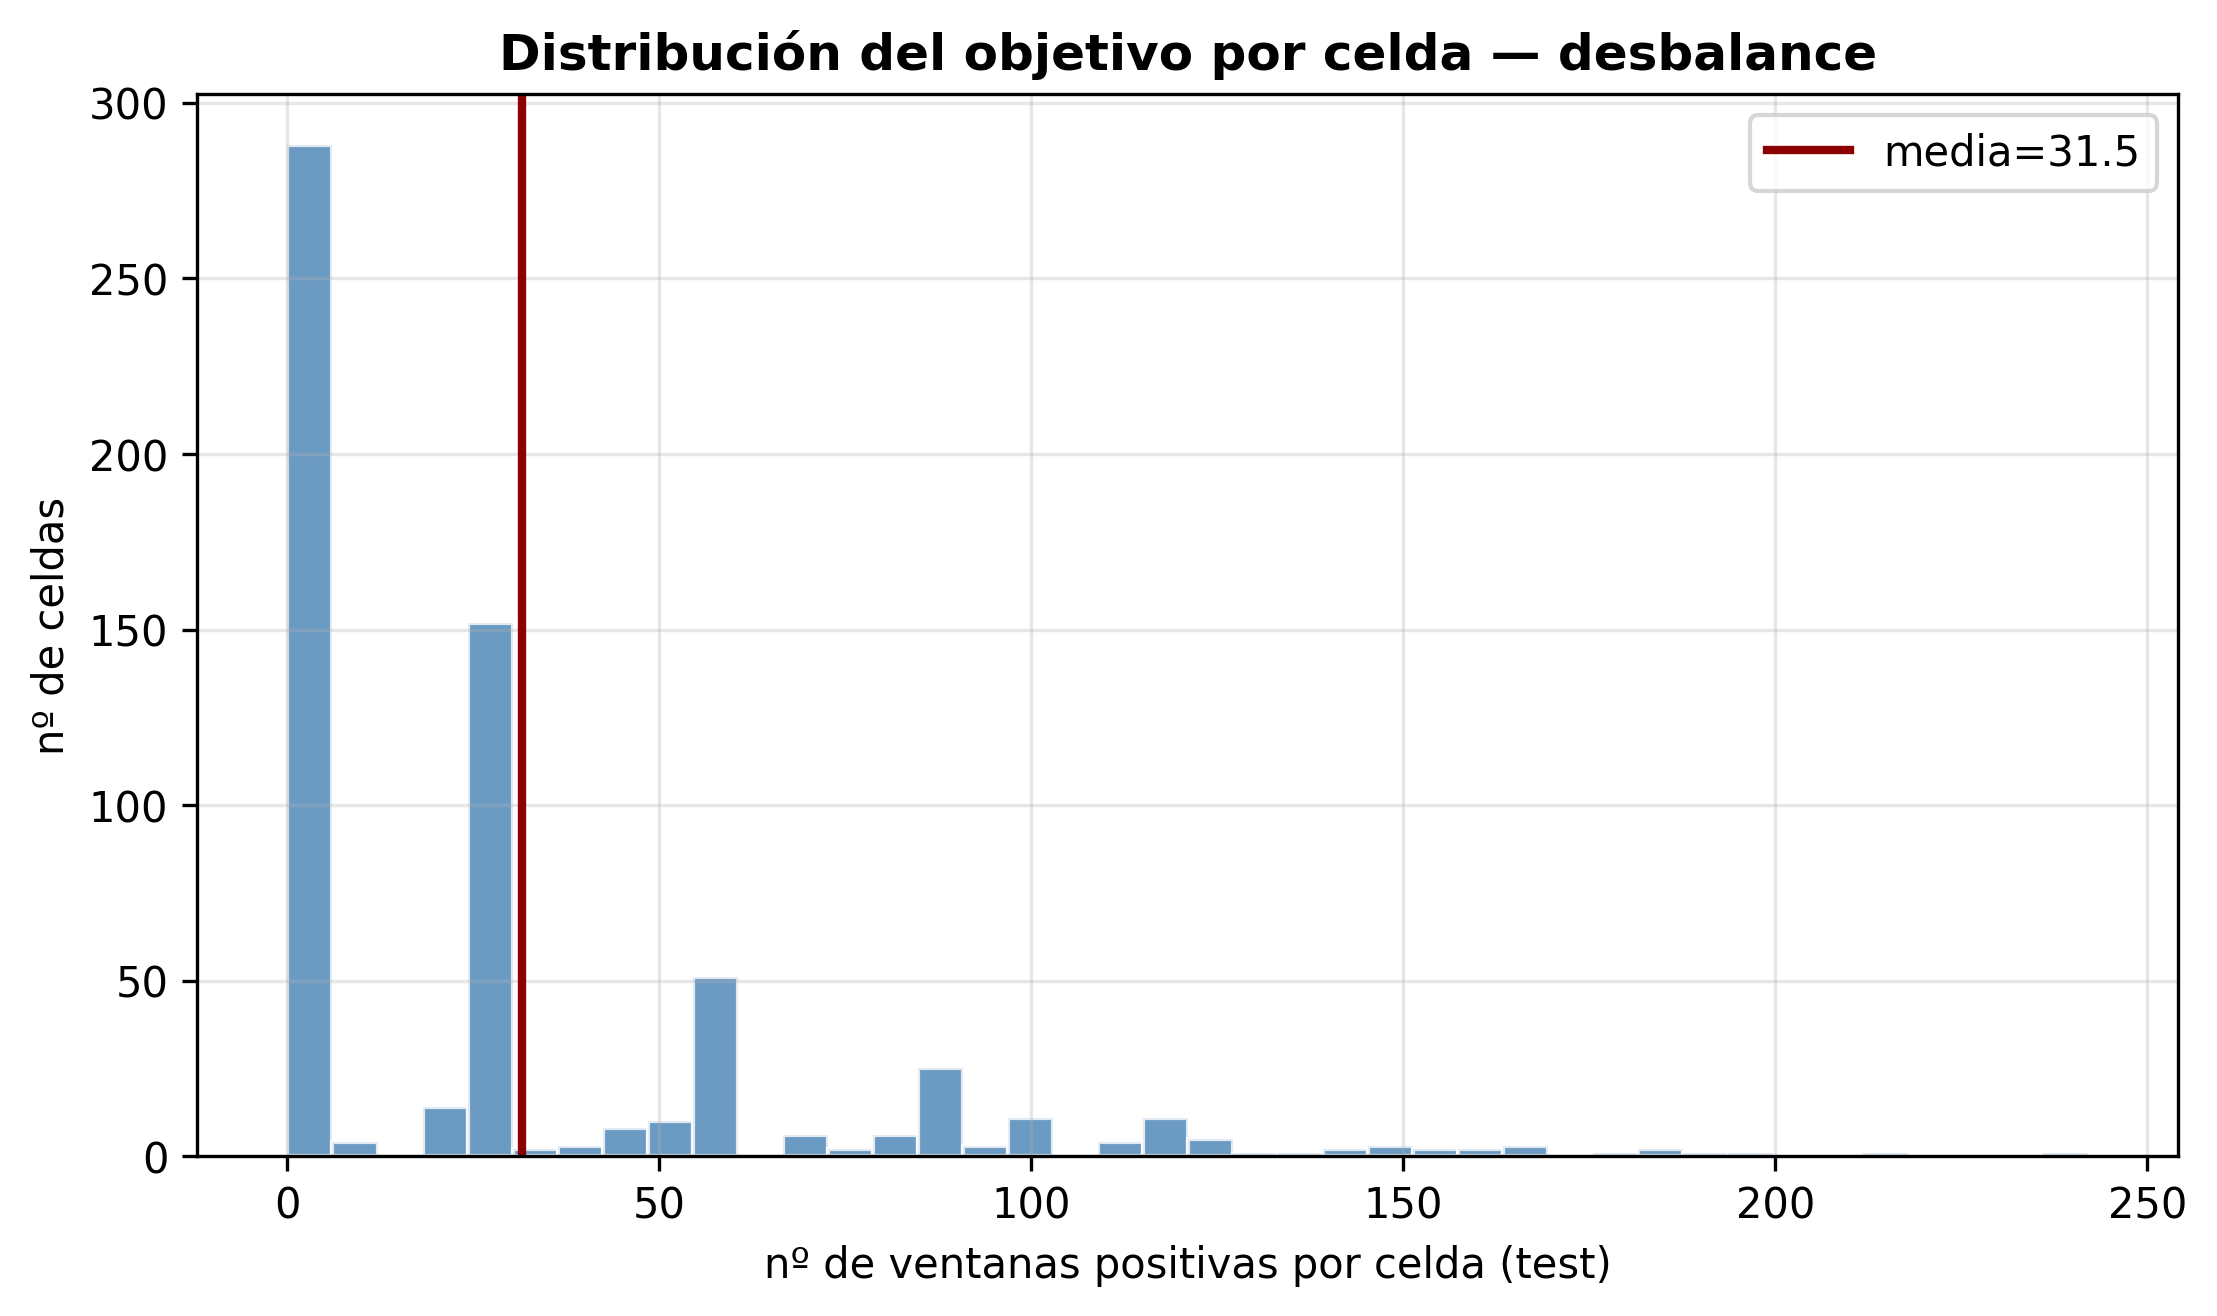
\includegraphics[width=0.78\textwidth]{figuras/04_desbalance}
  \caption[Distribución del objetivo por celda]{\textbf{Distribución del número de ventanas positivas por celda en el conjunto de test.} La mayoría de las celdas registran pocas ventanas con mainshock, mientras que unas pocas concentran la actividad. Este reparto desigual refleja el fuerte desbalance del problema.}
  \label{fig:desbalance}
\end{figure}

El segundo rasgo, más sutil, es que el problema encierra en realidad \textbf{dos preguntas
  distintas}: una espacial (¿qué zonas son peligrosas?) y otra temporal (¿cuándo lo serán?).
Estas dos preguntas tienen una dificultad muy distinta. La primera se apoya en una estructura
estable --las zonas sísmicamente activas lo son de forma persistente-- mientras que la segunda
exige anticipar el momento concreto de un evento, lo que es mucho más difícil. Gran parte del
trabajo de evaluación consiste precisamente en separar ambas, porque mezclarlas en una única
cifra puede dar una impresión equivocada del rendimiento del sistema.

% =============================================================================
\section{Desarrollo del proyecto}
\label{desarrollo-del-proyecto}

Esta sección recorre la construcción de las cinco fases del \textit{pipeline}. Para cada una
se describe qué se implementó y qué decisiones de diseño fueron relevantes; los valores
numéricos se presentan en la Sección~\ref{resultados}.

\subsection{Fase 1: detección y \textit{picking} de fases}
\label{dev-deteccion}

La primera fase valida las herramientas que permiten pasar de una forma de onda a un evento
catalogado. Se emplean dos redes preentrenadas sobre STEAD que representan dos familias
arquitectónicas distintas.

La primera, \textbf{PhaseNet}, es una red convolucional en forma de ``U'' (\textit{U-Net}).
Recibe la traza de tres componentes (las tres direcciones del movimiento del suelo) muestreada
a 100\,Hz y la procesa con una rama descendente de convoluciones y submuestreo, que extrae
características a escalas temporales cada vez más amplias, seguida de una rama ascendente de
sobremuestreo que reconstruye la resolución original. Las conexiones de salto entre ambas ramas
permiten combinar el detalle fino con el contexto global. La salida son tres canales de
probabilidad por cada instante de la traza --onda P, onda S y ruido-- de modo que la llegada de
cada fase se identifica como el máximo del canal correspondiente. Esta arquitectura es
especialmente precisa en la localización temporal, porque conserva la resolución de la señal de
entrada.

La segunda, \textbf{EQTransformer}, es una red más compleja que combina tres ingredientes:
convoluciones para extraer características locales, capas recurrentes bidireccionales que
recorren la traza en ambos sentidos y modelan dependencias de largo alcance, y un mecanismo de
atención que resalta las porciones de la señal relevantes para cada tarea. Su principal ventaja
es que resuelve \emph{tres} tareas a la vez con una sola pasada: detecta si hay un evento en la
traza y, en caso afirmativo, marca las llegadas de las ondas P y S. Esta naturaleza multitarea
la hace muy eficiente para procesar grandes volúmenes de señal continua.

Ambas redes se aplican \emph{sin reentrenar}, sobre un subconjunto de trazas de STEAD no usadas
en su entrenamiento original, y se evalúan comparando las llegadas predichas con las etiquetas
reales bajo varias tolerancias temporales. Esta fase responde a la pregunta de si las
herramientas modernas de detección funcionan de forma fiable sobre datos no vistos, paso previo
imprescindible para cualquier sistema de pronóstico.

El Algoritmo~\ref{alg:deteccion} describe el procedimiento de evaluación de la detección. Como
los modelos están preentrenados, no hay entrenamiento: el algoritmo recorre las trazas, ejecuta
el modelo en inferencia, convierte los canales de probabilidad en llegadas concretas, las
empareja con las llegadas reales dentro de una tolerancia y acumula los aciertos, los fallos y
los errores de tiempo con los que se calculan las métricas finales.

\begin{algorithm}[ht!]
  \caption{Evaluación de la detección y \textit{picking} de fases}
  \label{alg:deteccion}
  \DontPrintSemicolon
  \KwIn{Trazas de STEAD $\{W_i\}$ con llegadas reales de P y S; modelo preentrenado $\mathcal{M}$ (PhaseNet o EQTransformer); tolerancia $\tau$.}
  \KwOut{\textit{Precision}, \textit{recall}, F1 y errores de tiempo (MAE, RMSE) por fase.}
  Inicializar contadores $TP, FP, FN \leftarrow 0$ y lista de errores de tiempo\;
  \For{cada traza $W_i$}{
    $(p^{\text{P}}, p^{\text{S}}, p^{\text{ruido}}) \leftarrow \mathcal{M}(W_i)$ \tcp*{inferencia, sin reentrenar}
    \For{fase $\in \{\text{P}, \text{S}\}$}{
      $t_{\text{pred}} \leftarrow \arg\max_t\, p^{\text{fase}}(t)$ \tcp*{llegada = máximo del canal}
      \eIf{$\exists$ llegada real $t_{\text{real}}$ con $|t_{\text{pred}}-t_{\text{real}}| \leq \tau$}{
        $TP \mathrel{+}= 1$; registrar error $|t_{\text{pred}}-t_{\text{real}}|$\;
      }{
        $FP \mathrel{+}= 1$ (o $FN$ si no hubo predicción para una llegada real)\;
      }
    }
  }
  Calcular \textit{precision}, \textit{recall}, F1~\eqref{eq:f1}, MAE y RMSE\;
  \Return métricas por fase\;
\end{algorithm}

\subsection{Fase 2: red convolucional temporal global}
\label{dev-tcn}

La segunda fase aborda el pronóstico desde la dimensión puramente temporal. La TCN recibe
características agregadas de toda la región --concatenando las de California y las de Alaska--
y predice si habrá un mainshock en los próximos días en \emph{cualquier} punto de la zona. El
objetivo es comprobar si la evolución temporal de la sismicidad, por sí sola, contiene
información suficiente para anticipar eventos. Es, en cierto sentido, el experimento de
control del trabajo: si la señal estuviera en la dimensión temporal global, este modelo
debería capturarla.

Durante el desarrollo se observó un fenómeno relevante al ampliar la ventana de predicción. Al
unir California y Alaska, ambas muy activas, la pregunta ``¿habrá algún mainshock en toda la
región en los próximos 30 días?'' se vuelve casi siempre afirmativa, porque en una región tan
grande y activa suele ocurrir algún evento moderado en cualquier ventana de un mes. Esto
convierte el objetivo en degenerado y poco informativo, y motivó mantener la formulación global
con una ventana más corta. Este comportamiento ilustra por qué una formulación \emph{espacial},
que pregunta por celdas concretas en lugar de por toda la región, es más adecuada: en ella el
objetivo sí discrimina.

\subsection{Fase 3: red neuronal de grafos espacial}
\label{dev-gnn}

La tercera fase introduce la dimensión espacial. El modelo procesa la serie temporal de cada
celda con una TCN compartida y a continuación propaga información entre celdas vecinas mediante
dos capas de grafo, de modo que la predicción de una celda incorpora no solo su propia
historia, sino también la de su entorno. Esta fase pone a prueba la hipótesis de que la señal
aprovechable reside en los patrones espaciales locales y no en agregaciones globales. La
construcción del grafo, descrita en la Sección~\ref{md-grafo}, respeta la separación entre las
dos regiones.

En la implementación, el procesamiento se realiza por lotes de días completos: cada ejemplo de
entrenamiento es una ``foto'' de toda la región en un instante, con sus celdas y su grafo, lo
que permite que la propagación espacial actúe sobre el estado simultáneo de todas las celdas.
La matriz de adyacencia normalizada se precalcula una sola vez, ya que el grafo es fijo, lo que
hace muy eficiente cada paso de propagación. El número de parámetros se mantiene en el orden de
las decenas de miles gracias a que la TCN comparte pesos entre todas las celdas; esta economía
de parámetros es deliberada y especialmente importante en un problema con relativamente pocos
ejemplos positivos, porque reduce el riesgo de sobreajuste. Durante el desarrollo se comprobó
que la profundidad de dos capas de grafo ofrece el mejor equilibrio: con una sola capa la
información apenas se propaga, y con más de dos aparece el fenómeno de sobre-suavizado, por el
que las celdas tienden a parecerse entre sí y se pierde la discriminación local.

\subsection{Fase 4: Transformer geoespacial}
\label{dev-transformer}

La cuarta fase explora una segunda forma de modelar el espacio. En lugar de imponer un grafo de
vecindad fijo, el Transformer deja que el mecanismo de atención aprenda qué celdas son
relevantes para cada predicción, usando la codificación de las coordenadas geográficas. Comparte
el mismo procesamiento temporal que la GNN, de modo que la comparación entre ambos aísla el
efecto del mecanismo de mezcla espacial. Durante el desarrollo se introdujeron dos mejoras que
resultaron beneficiosas: el uso del \textit{pooling} temporal completo (estado final, media y
máximo) a la entrada del bloque de atención, y la máscara que restringe la atención al interior
de cada región. Con ellas, el Transformer se convirtió en el modelo espacial con mejor
rendimiento del trabajo.

La diferencia conceptual con la GNN merece subrayarse. La red de grafos parte de una hipótesis
fuerte --que las celdas relevantes son las geográficamente próximas-- y la codifica en un grafo
fijo. El Transformer, en cambio, no impone esa hipótesis: deja que los datos decidan, para cada
celda, a cuáles otras conviene atender, ponderando su contribución mediante pesos aprendidos. La
codificación posicional sinusoidal de las coordenadas le proporciona el sentido de la geografía
que el grafo le daba de forma explícita a la GNN, pero de manera más flexible. La máscara por
regiones actúa como una restricción mínima e indiscutible --no tiene sentido que una celda de
California atienda a una de Alaska-- que reduce el espacio de búsqueda y estabiliza el
entrenamiento sin imponer una estructura de vecindad rígida. El hecho de que esta mayor
flexibilidad se traduzca en un rendimiento ligeramente superior sugiere que la noción de
``vecindad relevante'' en sismicidad es algo más rica que la simple proximidad geográfica.

\subsection{Fase 5: Proceso Gaussiano y mapas de riesgo}
\label{dev-gp}

La quinta fase cierra el \textit{pipeline} transformando las predicciones discretas por celda
en un producto cartográfico. El proceso gaussiano interpola las probabilidades sobre una
rejilla fina, produciendo una superficie continua de riesgo, y aporta además una estimación de
incertidumbre en cada punto. El procedimiento consta de tres pasos encadenados. Primero, se
toman las probabilidades del Transformer en los centroides de las celdas activas y se promedian
sobre el periodo de evaluación para obtener un valor de riesgo representativo por celda.
Segundo, esas probabilidades se \emph{calibran} mediante regresión isotónica, una técnica que
ajusta una función monótona para que las probabilidades predichas coincidan con las frecuencias
observadas; este paso es necesario porque la ponderación de clase usada en el entrenamiento
infla las probabilidades crudas, y la calibración se ajusta sobre una mitad del test y se valida
sobre la otra para evitar circularidad. Tercero, el proceso gaussiano interpola esos valores
calibrados sobre una rejilla fina, ajustando los parámetros de su \textit{kernel} de Matérn por
máxima verosimilitud de forma independiente en cada región. El resultado son dos mapas por
región: uno de riesgo y otro de
incertidumbre.

El Algoritmo~\ref{alg:gp} recoge estos tres pasos --promediado, calibración e interpolación--
y muestra cómo el proceso gaussiano entrega a la vez el mapa de riesgo (su media) y el de
incertidumbre (su desviación) en cada punto de la rejilla.

\begin{algorithm}[ht!]
  \caption{Cartografía del riesgo con calibración y Proceso Gaussiano}
  \label{alg:gp}
  \DontPrintSemicolon
  \KwIn{Probabilidades del Transformer por celda y día; centroides de las celdas activas; rejilla fina de salida.}
  \KwOut{Mapa de riesgo y mapa de incertidumbre por región.}
  $\bar{p}_c \leftarrow$ media temporal de la probabilidad en cada celda $c$ \tcp*{un valor por celda}
  Ajustar la regresión isotónica $g(\cdot)$ en una mitad del test; validar en la otra\;
  $r_c \leftarrow g(\bar{p}_c)$ \tcp*{probabilidades calibradas}
  \For{cada región (California, Alaska)}{
    Ajustar el GP (\textit{kernel} Matérn) por máxima verosimilitud sobre $\{(\text{centroide}_c, r_c)\}$\;
    \For{cada punto $\mathbf{x}_*$ de la rejilla}{
      $\mu_* \leftarrow \mathbf{k}_*^\top (K+\sigma^2 I)^{-1} \mathbf{r}$ \tcp*{riesgo interpolado}
      $\sigma_*^2 \leftarrow k(\mathbf{x}_*,\mathbf{x}_*) - \mathbf{k}_*^\top (K+\sigma^2 I)^{-1}\mathbf{k}_*$ \tcp*{incertidumbre}
    }
  }
  \Return mapa de riesgo $\mu$ y mapa de incertidumbre $\sigma$\;
\end{algorithm}

% =============================================================================
\section{Resultados}
\label{resultados}

Esta sección presenta los resultados de las cinco fases. Se comienza por la detección, se
continúa con la comparación de los modelos de pronóstico y su análisis espacial y temporal, se
añaden las métricas operativas y los estudios de ablación, y se cierra con los mapas de riesgo
y la discusión de los resultados en el contexto del estado del arte.

\subsection{Detección y \textit{picking} de fases}
\label{res-deteccion}

La Tabla~\ref{tab:deteccion} recoge el rendimiento de PhaseNet y EQTransformer en la
identificación de las llegadas de las ondas P y S, con una tolerancia de 0.1\,s. Ambas redes
alcanzan un rendimiento alto, especialmente en la onda P, que es la más nítida. PhaseNet obtiene
un \textit{F1-score}~\eqref{eq:f1} de 0.93 en la fase P y de 0.79 en la fase S, con errores
medios de localización de pocas centésimas de segundo, comparables a los de un analista humano.
EQTransformer ofrece un rendimiento ligeramente inferior en este subconjunto pero igualmente
sólido, con la ventaja de resolver las tres tareas (detección, P y S) en una sola pasada.

\begin{table}[ht!]
  \centering
  \small
  \begin{tabular}{@{}llccccc@{}}
    \toprule
    \textbf{Modelo} & \textbf{Fase} & \textbf{Precision} & \textbf{Recall} & \textbf{F1}    & \textbf{MAE (s)} & \textbf{RMSE (s)} \\
    \midrule
    PhaseNet        & P             & 0.927              & 0.934           & \textbf{0.930} & 0.022            & 0.030             \\
    PhaseNet        & S             & 0.782              & 0.794           & 0.788          & 0.029            & 0.038             \\
    EQTransformer   & P             & 0.883              & 0.787           & 0.832          & 0.027            & 0.036             \\
    EQTransformer   & S             & 0.739              & 0.760           & 0.750          & 0.035            & 0.044             \\
    \bottomrule
  \end{tabular}
  \caption[Resultados de detección y \textit{picking} de fases P y S]{\textbf{Rendimiento en detección y \textit{picking}} de PhaseNet y EQTransformer sobre STEAD (tolerancia 0.1\,s). MAE y RMSE son los errores de localización temporal de la llegada, en segundos.}
  \label{tab:deteccion}
\end{table}

Estos resultados confirman que las herramientas de detección basadas en aprendizaje profundo funcionan
de forma fiable sobre datos no vistos y constituyen una base firme sobre la que apoyar el resto
del sistema.

\begin{figure}[ht!]
  \centering
  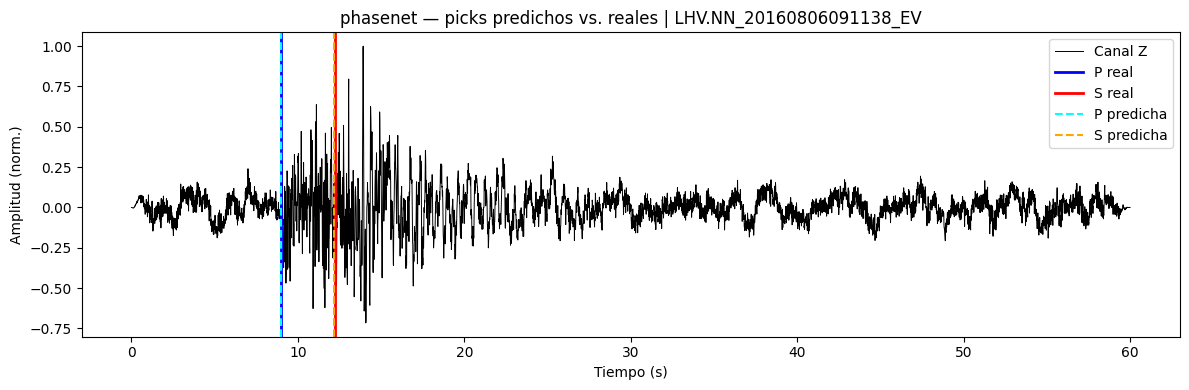
\includegraphics[width=0.92\textwidth]{figuras/output_phasnet}
  \caption[Ejemplo de detección y \textit{picking} con PhaseNet]{\textbf{Ejemplo de detección y \textit{picking} con PhaseNet} sobre una traza de STEAD. Se muestran las componentes de la forma de onda junto con las probabilidades de fase predichas por la red y las llegadas estimadas de las ondas P y S.}
  \label{fig:output-phasenet}
\end{figure}

\begin{figure}[ht!]
  \centering
  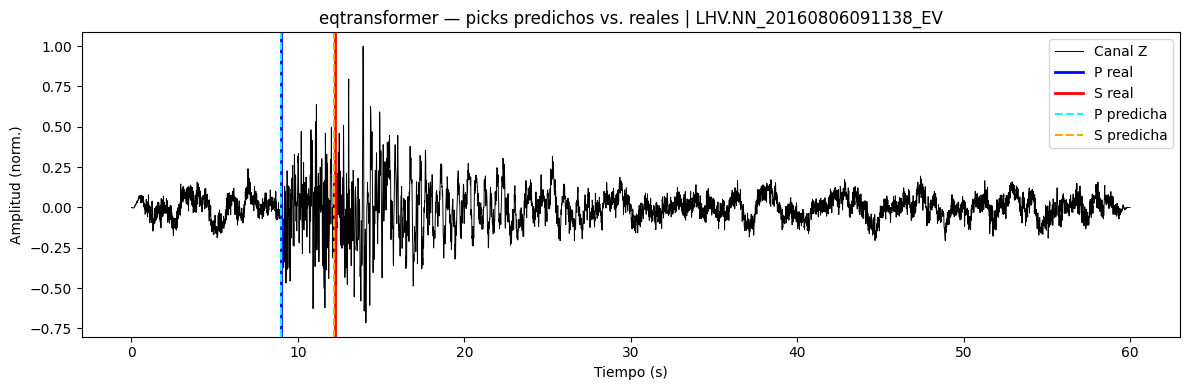
\includegraphics[width=0.92\textwidth]{figuras/output_eqtransformer}
  \caption[Ejemplo de detección y \textit{picking} con EQTransformer]{\textbf{Ejemplo de detección y \textit{picking} con EQTransformer} sobre una traza de STEAD. Junto a la forma de onda se representan las probabilidades de detección del evento y de las llegadas de las ondas P y S obtenidas en una sola pasada.}
  \label{fig:output-eqtransformer}
\end{figure}

La tolerancia de 0.1\,s es exigente: equivale a acertar la llegada con un margen de diez
muestras a 100\,Hz. Conviene comprobar cómo evoluciona el rendimiento al relajar este margen,
porque en muchas aplicaciones operativas un error de unas décimas de segundo es perfectamente
asumible. La Tabla~\ref{tab:deteccion-umbral} recoge el \textit{F1-score} de la fase P de
PhaseNet para tres tolerancias. Como cabe esperar, el rendimiento crece al ampliar la
tolerancia: con un margen de medio segundo el \textit{F1} supera el 0.96, lo que confirma que
la inmensa mayoría de las llegadas se detectan correctamente y que los pocos fallos a tolerancia
estricta corresponden a pequeñas desviaciones en la localización, no a detecciones perdidas.

\begin{table}[ht!]
  \centering
  \small
  \begin{tabular}{@{}lccc@{}}
    \toprule
    \textbf{Tolerancia} & \textbf{0.1\,s} & \textbf{0.3\,s} & \textbf{0.5\,s} \\
    \midrule
    \textit{F1} fase P  & 0.930           & 0.951           & 0.963           \\
    \bottomrule
  \end{tabular}
  \caption[Sensibilidad de la detección a la tolerancia temporal]{\textbf{\textit{F1-score} de la fase P (PhaseNet) según la tolerancia temporal.} Al relajar el margen de acierto, el rendimiento aumenta, lo que indica que los errores se concentran en pequeñas desviaciones de localización y no en detecciones omitidas.}
  \label{tab:deteccion-umbral}
\end{table}

\subsection{Comparación de los modelos de pronóstico}
\label{res-comparativa}

La Tabla~\ref{tab:comparativa} reúne el rendimiento de todos los modelos de pronóstico sobre el
conjunto de test (2023--2024), junto con las tres referencias. Todos los modelos espaciales se
evalúan sobre el mismo objetivo, de modo que las cifras son directamente comparables. Para los
modelos con varias semillas se indica la media y la desviación típica.

\begin{table}[ht!]
  \centering
  \small
  \begin{tabular}{@{}lcc@{}}
    \toprule
    \textbf{Modelo}               & \textbf{AUC-ROC (test)}    & \textbf{Tipo}       \\
    \midrule
    Persistencia                  & 0.513                      & referencia temporal \\
    Regresión logística           & 0.544                      & referencia lineal   \\
    TCN global (Fase 2)           & 0.512 $\pm$ 0.052          & temporal            \\
    \midrule
    Poisson (climatología)        & 0.726                      & referencia espacial \\
    GNN (Fase 3)                  & 0.699 $\pm$ 0.008          & espacial            \\
    \textbf{Transformer (Fase 4)} & \textbf{0.728 $\pm$ 0.002} & espacial            \\
    \bottomrule
  \end{tabular}
  \caption[Comparativa de los modelos de pronóstico frente a las referencias]{\textbf{Resultados de pronóstico en test (2023--2024).} AUC-ROC de cada modelo frente a las referencias. La persistencia, la regresión logística y el TCN operan sobre objetivos globales o lineales; los modelos espaciales y el Poisson comparten el objetivo por celda. Para los modelos entrenados con varias semillas, el valor es la media y el \(\pm\) la \textbf{desviación típica muestral} (dividiendo entre \(N-1\)) del AUC sobre las cinco semillas \{13, 42, 123, 256, 1024\}.}
  \label{tab:comparativa}
\end{table}

Los resultados permiten una lectura clara. En el bloque temporal, ni la persistencia, ni la
regresión logística, ni el TCN superan de forma apreciable el nivel del azar: el TCN global
alcanza un AUC de 0.512 y un test estadístico confirma que no mejora a la regresión logística
de manera significativa. Esto indica que la dimensión temporal global, por sí sola, no contiene
información suficiente para el pronóstico, y justifica el paso a una formulación espacial. La
Figura~\ref{fig:roctcn} lo ilustra: las curvas ROC del TCN se mantienen muy próximas a la
diagonal del azar.

\begin{figure}[ht!]
  \centering
  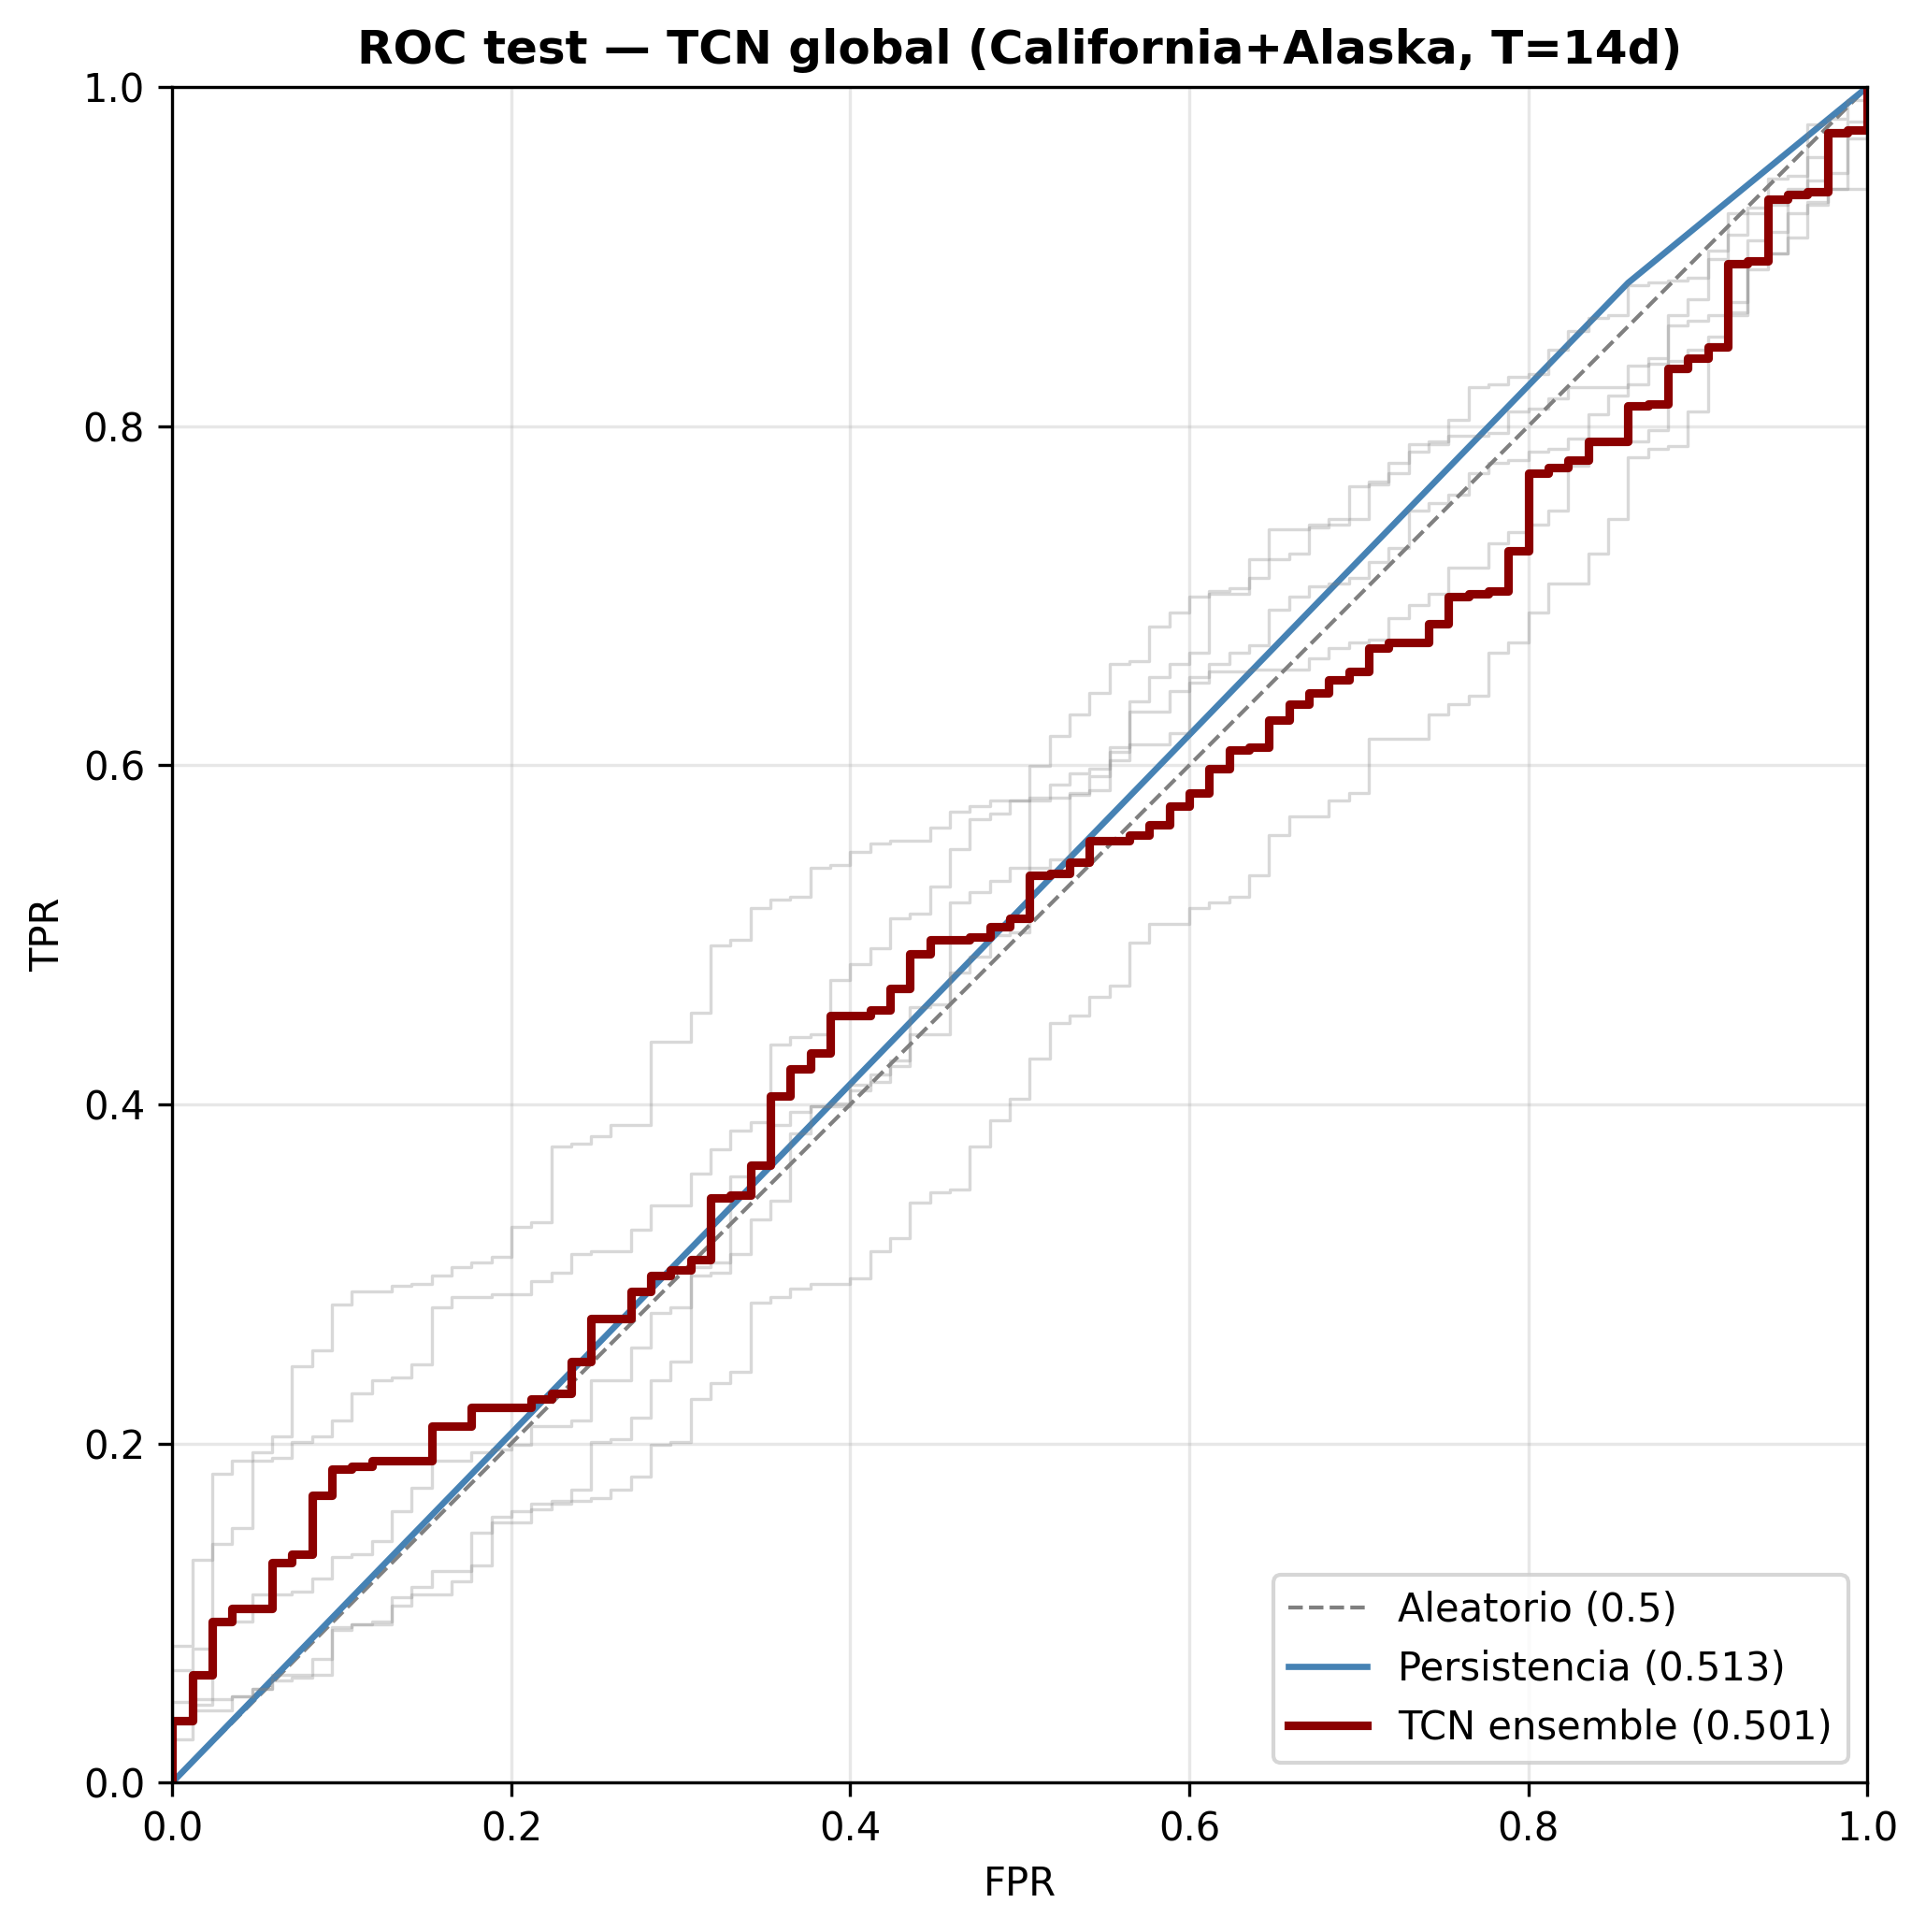
\includegraphics[width=0.64\textwidth]{figuras/03_roc_test}
  \caption[Curva ROC del TCN temporal global]{\textbf{Curvas ROC en test del TCN temporal global.} En gris, las cinco semillas; en rojo, el \textit{ensemble}; en azul, la persistencia. La proximidad a la diagonal indica que el enfoque temporal global no aporta capacidad discriminativa.}
  \label{fig:roctcn}
\end{figure}

En el bloque espacial el panorama cambia. Tanto la GNN como el Transformer alcanzan un AUC en
torno a 0.70--0.73, muy por encima de las referencias temporales. El \textbf{Transformer es
  el mejor modelo}, con un AUC de \(0.728 \pm 0.002\) que supera a la climatología de Poisson de
forma estadísticamente significativa: un \emph{t}-test de una muestra de las cinco semillas
frente a la tasa base del Poisson da \(t = 2.6\) y \(p = 0.029\) (contraste unilateral). La GNN,
con \(0.699\), queda ligeramente por debajo del Poisson. La superioridad del Transformer sobre la
GNN también se confirma con un test no paramétrico: un \textbf{Wilcoxon pareado} sobre las cinco
semillas comunes --donde el Transformer gana a la GNN en las cinco-- arroja \(p = 0.031\)
(unilateral); el equivalente \emph{t}-test pareado, más potente con tan pocas muestras, da
\(p = 0.001\). La estabilidad de estos resultados se aprecia en la
Tabla~\ref{tab:perseed}, que detalla el AUC de cada semilla: la desviación típica es muy pequeña,
del orden de la milésima en el Transformer, lo que indica que los valores no dependen del azar de
una ejecución concreta sino que son una propiedad robusta del modelo y de los datos. De hecho, el
\textbf{intervalo de confianza al 95\,\%} del AUC, estimado con la distribución \emph{t} de
Student sobre las cinco semillas, es estrecho y no incluye al azar: \([0.725,\,0.731]\) para el
Transformer y \([0.690,\,0.709]\) para la GNN. La Figura~\ref{fig:curvas} muestra las curvas de
entrenamiento del Transformer, con una convergencia muy consistente entre semillas.

\begin{table}[ht!]
  \centering
  \small
  \begin{tabular}{@{}lccccccc@{}}
    \toprule
    \textbf{Modelo} & \textbf{s.\,13} & \textbf{s.\,42} & \textbf{s.\,123} & \textbf{s.\,256} & \textbf{s.\,1024} & \textbf{media\(\pm\)std} & \textbf{ens.} \\
    \midrule
    GNN             & 0.694           & 0.703           & 0.711            & 0.694            & 0.694             & 0.699\(\pm\)0.008        & 0.702         \\
    Transformer     & 0.732           & 0.728           & 0.728            & 0.726            & 0.726             & 0.728\(\pm\)0.002        & 0.729         \\
    \bottomrule
  \end{tabular}
  \caption[AUC de test por semilla de los modelos espaciales]{\textbf{AUC-ROC en test para cada semilla.} La baja dispersión entre semillas confirma que los resultados son estables y reproducibles. La columna media\(\pm\)std recoge la media y la \textbf{desviación típica muestral} (\(N-1\)) sobre las cinco semillas; el \textit{ensemble} promedia las cinco predicciones.}
  \label{tab:perseed}
\end{table}

\begin{figure}[ht!]
  \centering
  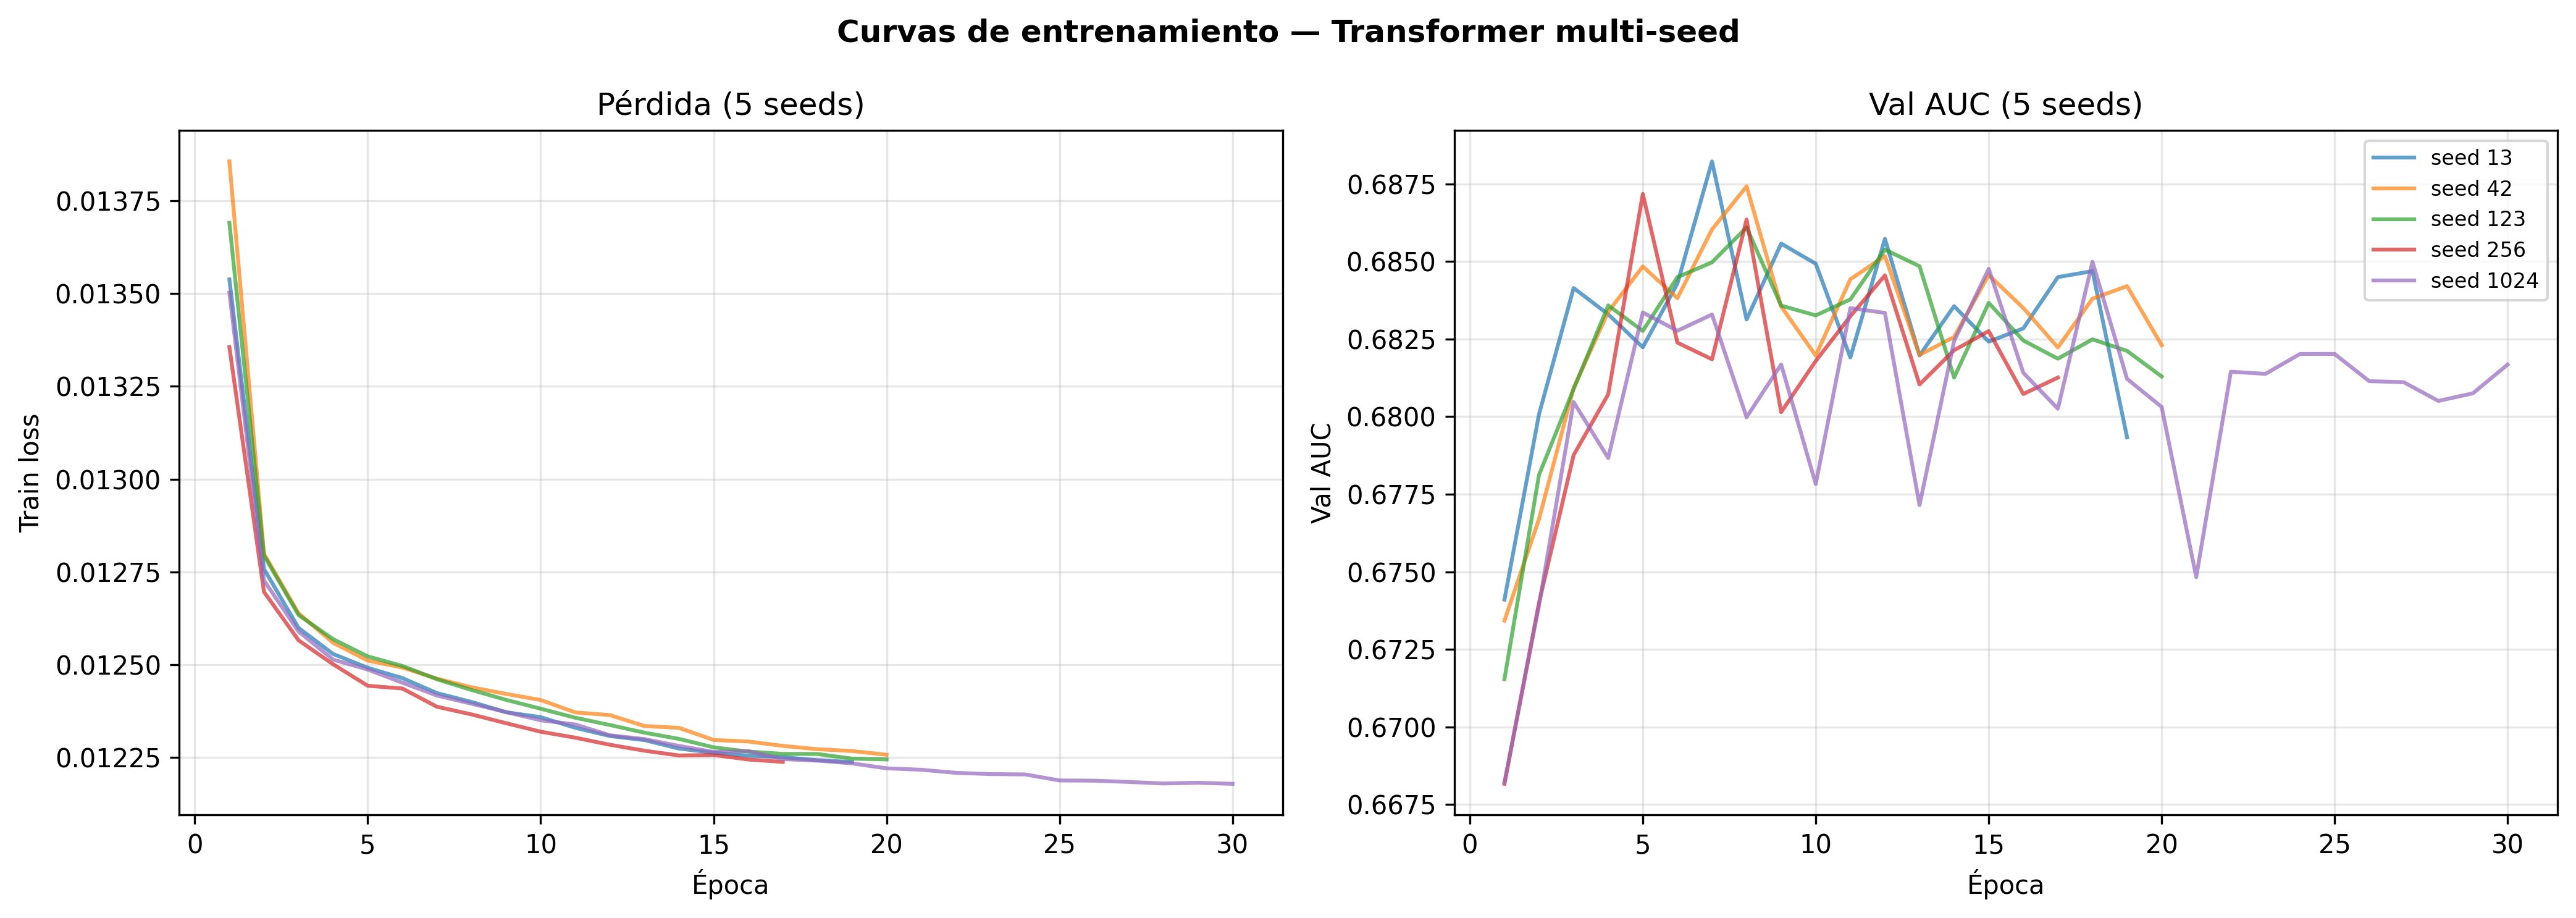
\includegraphics[width=\textwidth]{figuras/05_curvas_multiseed}
  \caption[Curvas de entrenamiento del Transformer multi-semilla]{\textbf{Curvas de entrenamiento del Transformer} para las cinco semillas. Izquierda: pérdida de entrenamiento. Derecha: AUC de validación por época. La convergencia consistente entre semillas refleja un entrenamiento estable.}
  \label{fig:curvas}
\end{figure}

Para visualizar de un vistazo cómo se sitúan los tres modelos espaciales, la
Figura~\ref{fig:comparativa} compara sus métricas en dos paneles. El panel de la izquierda
muestra la capacidad discriminativa (AUC-ROC y PR-AUC) y el de la derecha el rendimiento
operativo (\textit{lift} en los dos niveles de alarma). La lectura conjunta es clara: el
Transformer y el Poisson van prácticamente a la par y por delante de la GNN en todas las
métricas. La diferencia es especialmente visible en el \textit{lift} y en la PR-AUC, donde la
GNN se queda algo por detrás de la climatología, mientras que el Transformer la iguala o la
supera ligeramente. Esta figura resume el mensaje central de la comparación: el Transformer es
el modelo de aprendizaje profundo que logra ponerse al nivel de la mejor referencia y rebasarla.

\begin{figure}[ht!]
  \centering
  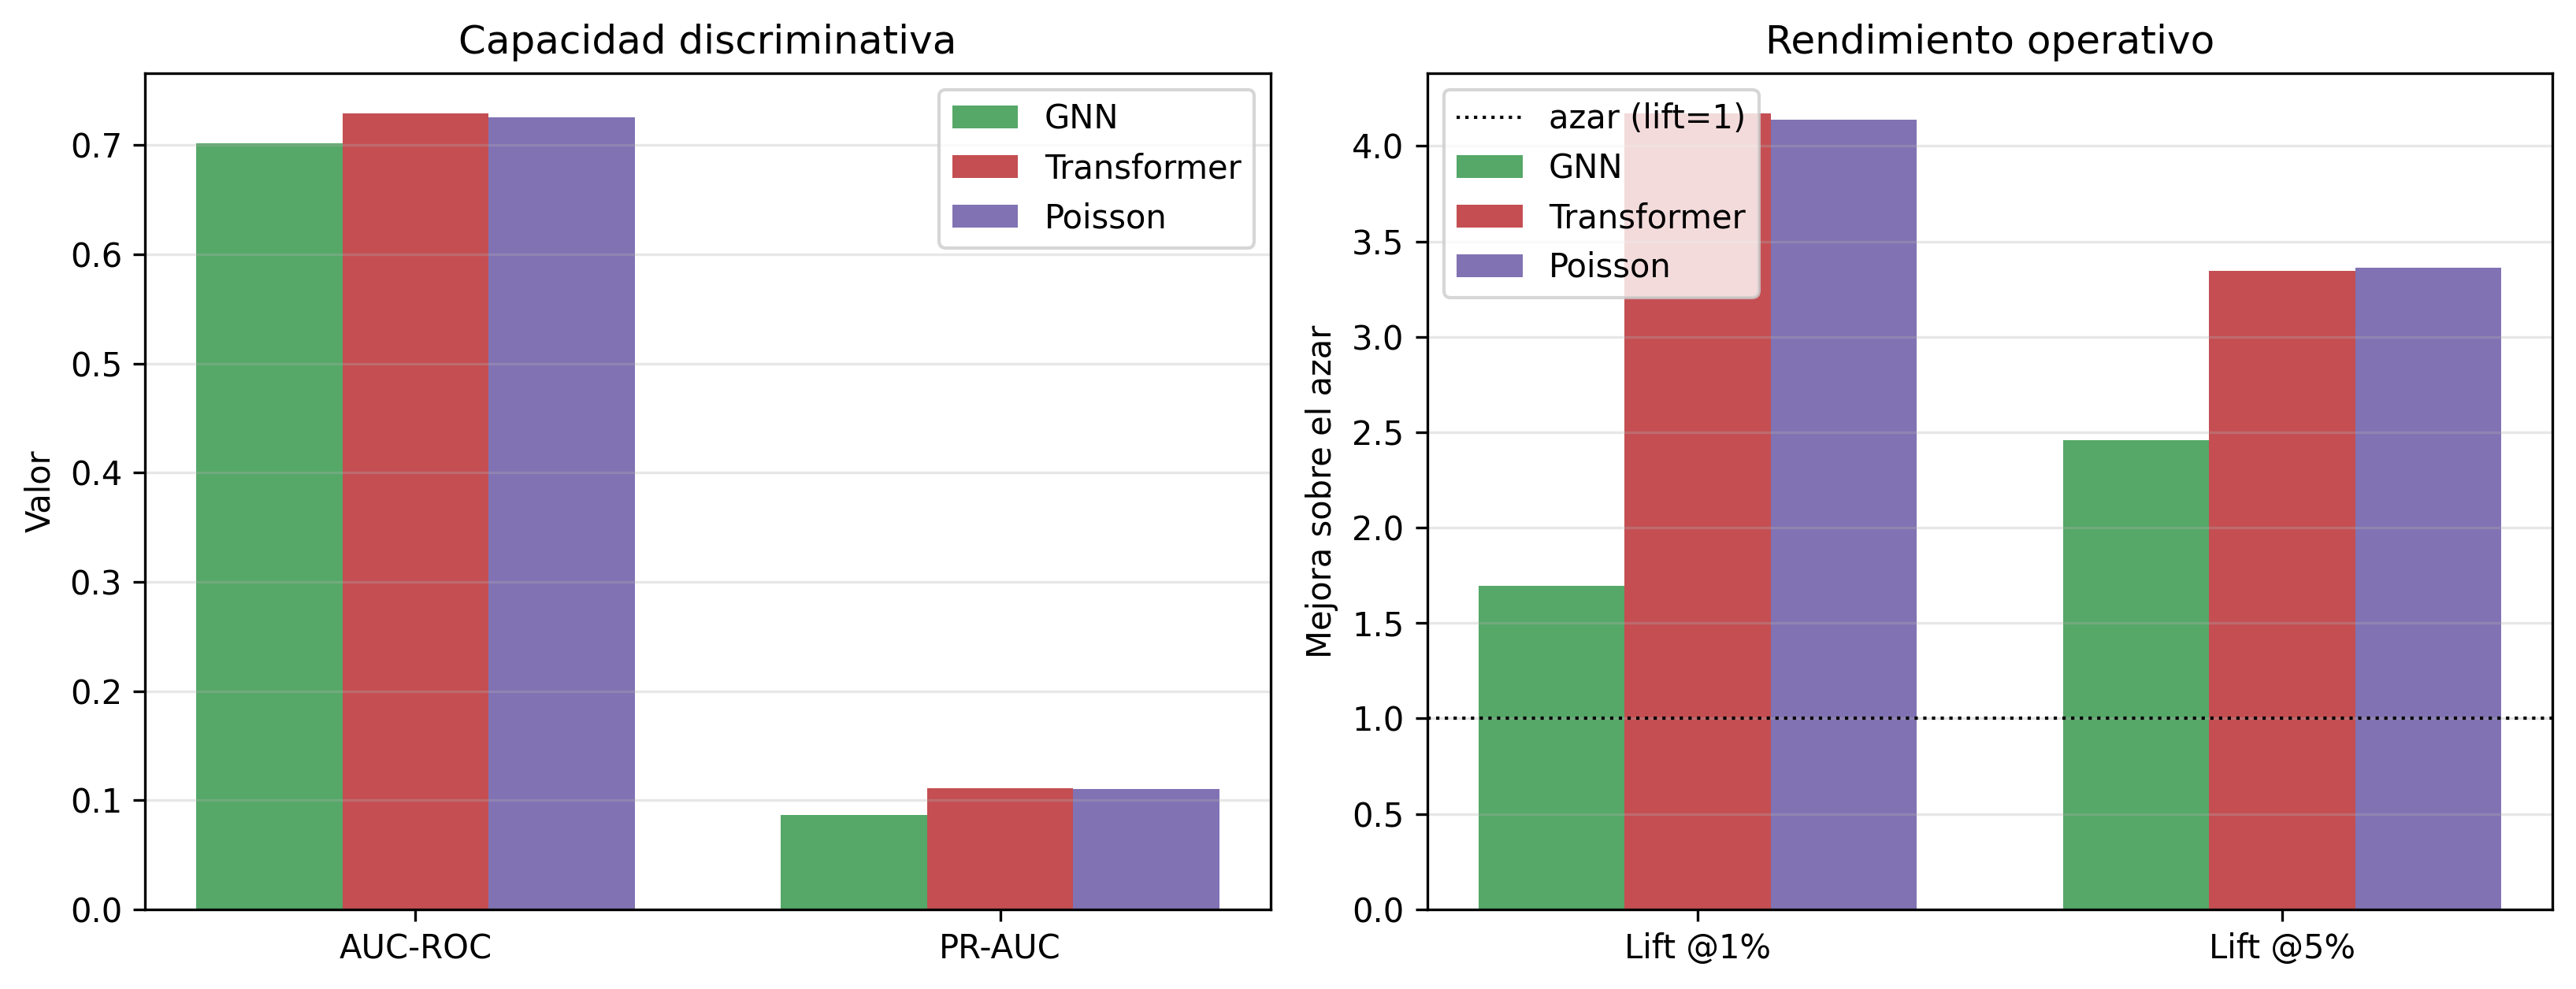
\includegraphics[width=\textwidth]{figuras/comparativa_modelos}
  \caption[Comparativa de métricas entre modelos espaciales]{\textbf{Comparativa de métricas de los modelos espaciales frente al Poisson.} Izquierda: capacidad discriminativa (AUC-ROC y PR-AUC). Derecha: rendimiento operativo (\textit{lift} en el top 1\,\% y 5\,\%; la línea de puntos marca el azar). El Transformer iguala o supera a la climatología en todas las métricas, mientras que la GNN queda algo por detrás.}
  \label{fig:comparativa}
\end{figure}

\subsection{Curvas ROC y diagrama de Molchan}
\label{res-roc-molchan}

La Figura~\ref{fig:roc} muestra las curvas ROC del Transformer y del Poisson sobre el test. Ambas
quedan claramente por encima de la diagonal del azar, lo que refleja una capacidad de
discriminación apreciable. La Figura~\ref{fig:molchan} presenta el mismo resultado en el formato
del diagrama de Molchan, habitual en sismología: la curva del Transformer cae por debajo de la
diagonal, señal de un \textit{skill} positivo, y muy próxima a la del Poisson.

\begin{figure}[ht!]
  \centering
  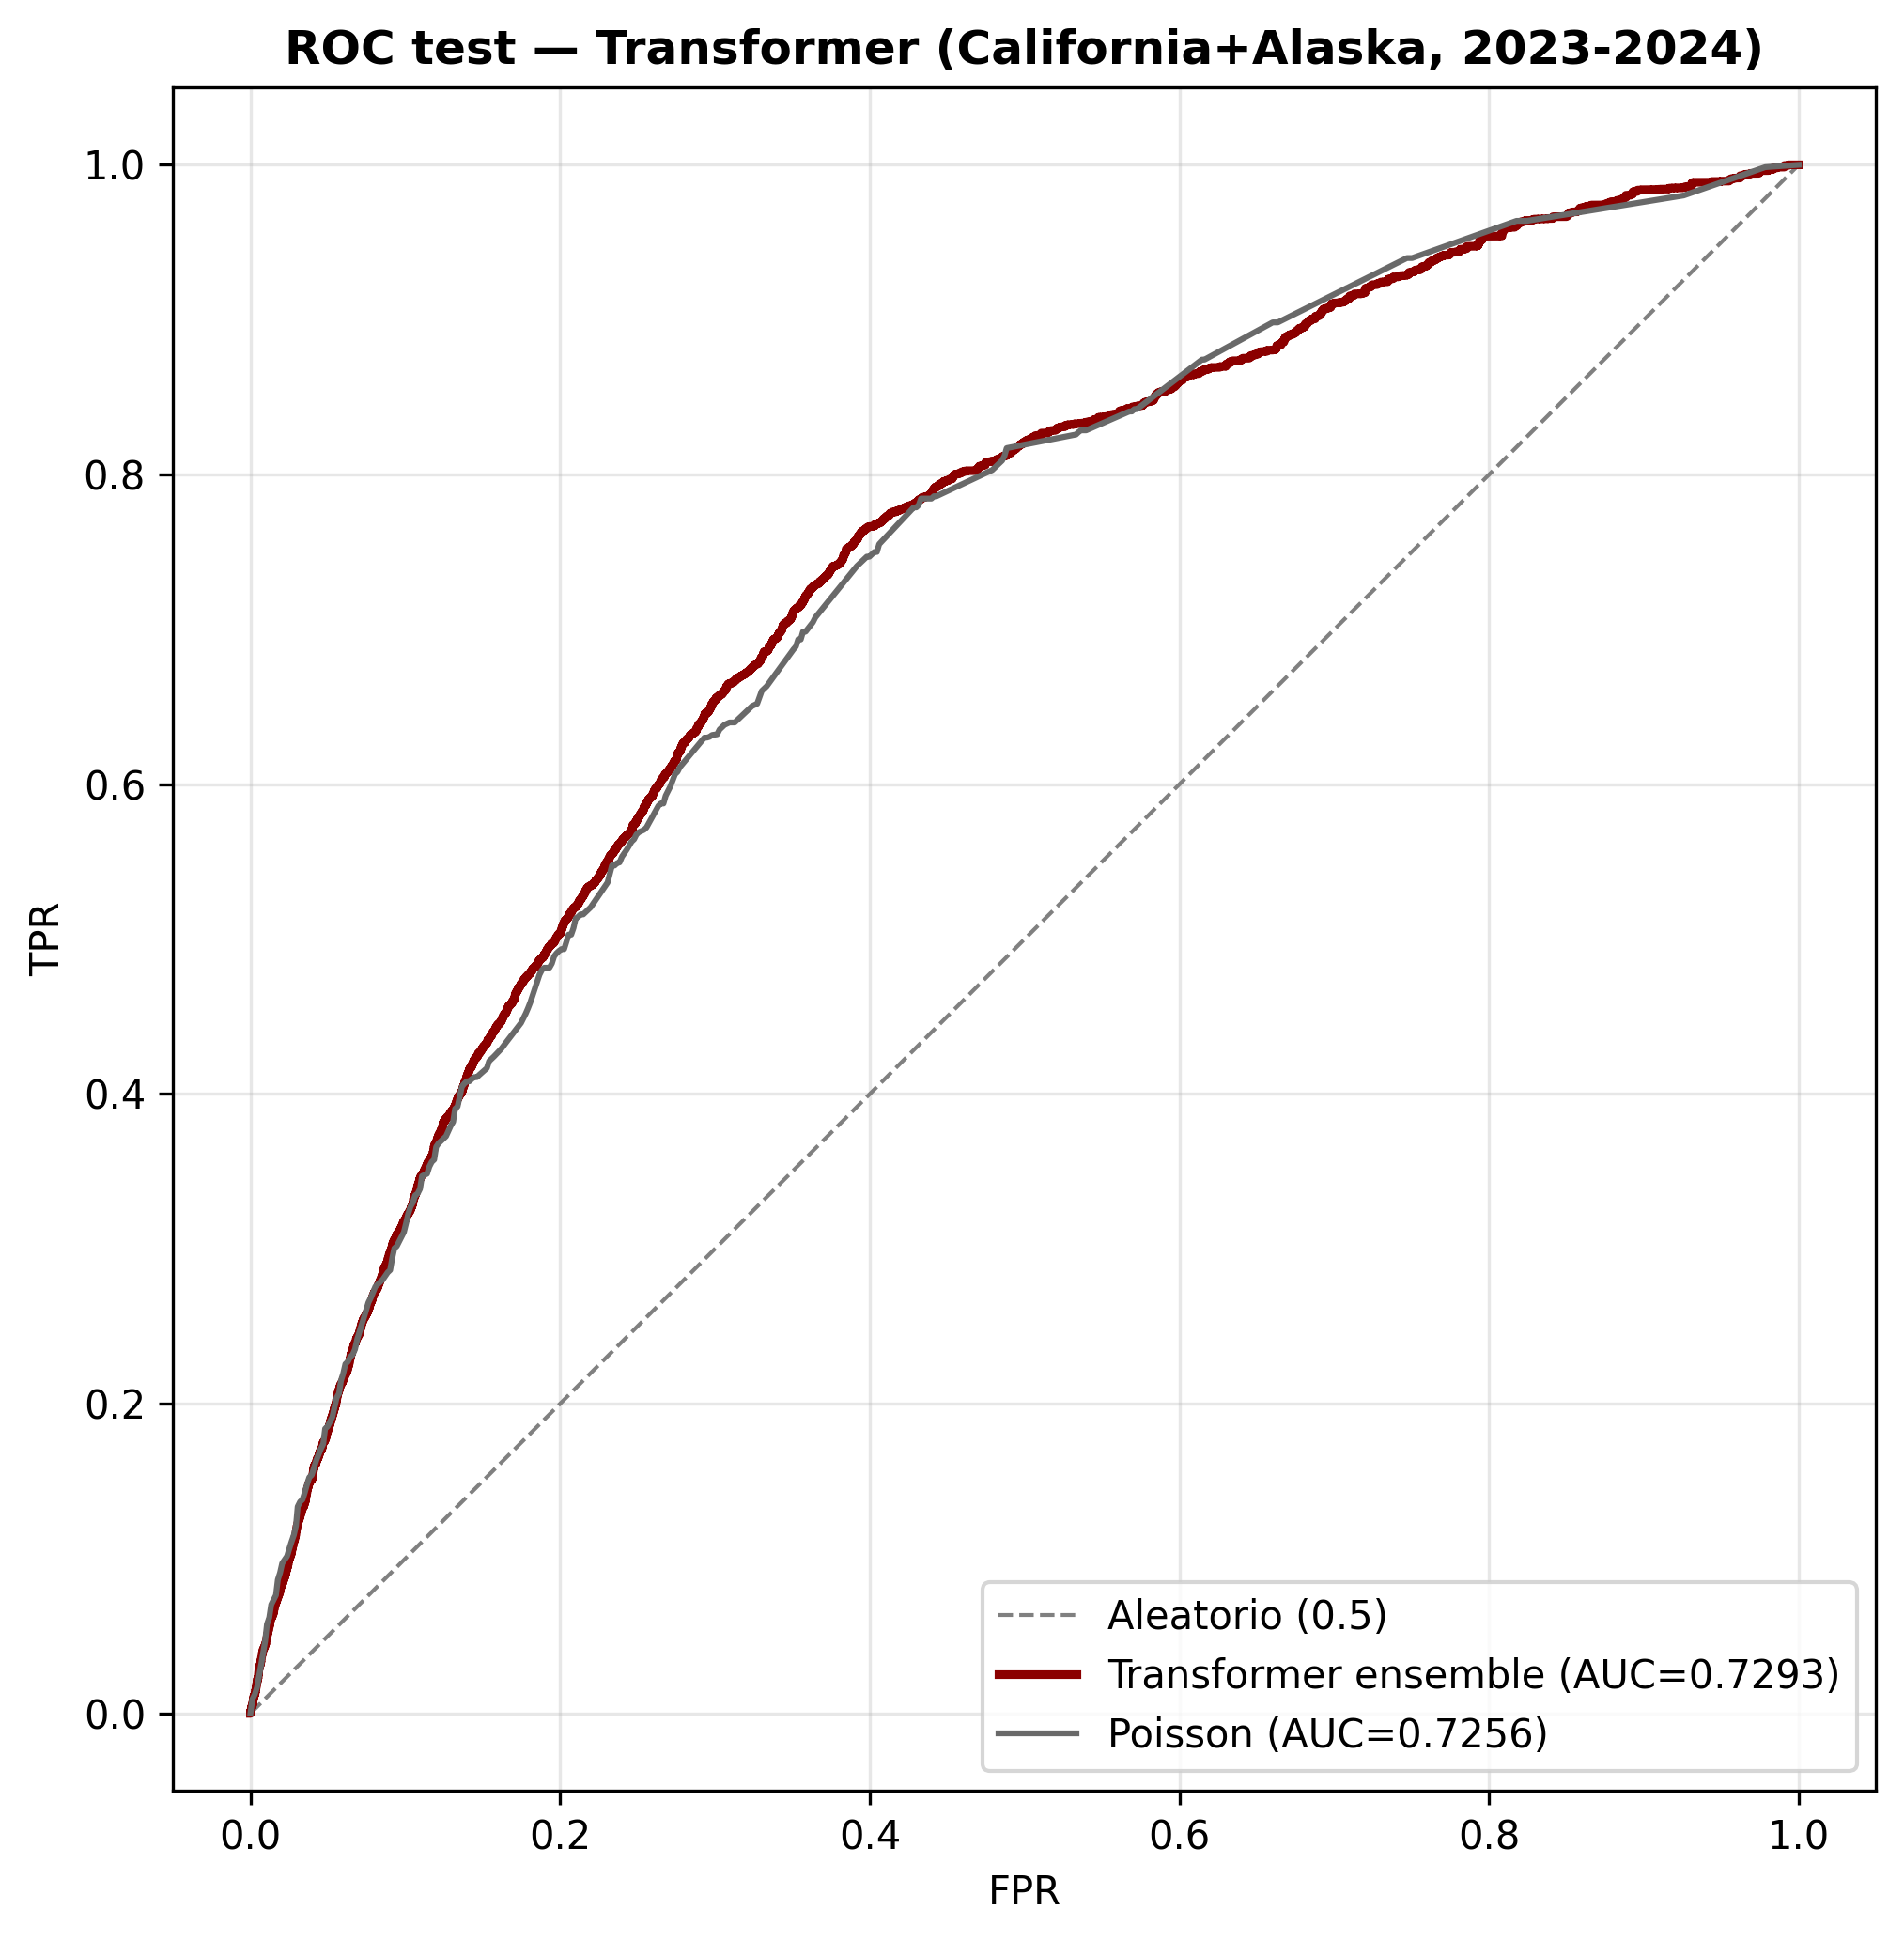
\includegraphics[width=0.66\textwidth]{figuras/05_roc_test}
  \caption[Curva ROC del Transformer en test]{\textbf{Curva ROC en test (2023--2024)} del \textit{ensemble} del Transformer geoespacial frente al modelo de Poisson. Ambos superan claramente la diagonal del azar.}
  \label{fig:roc}
\end{figure}

\begin{figure}[ht!]
  \centering
  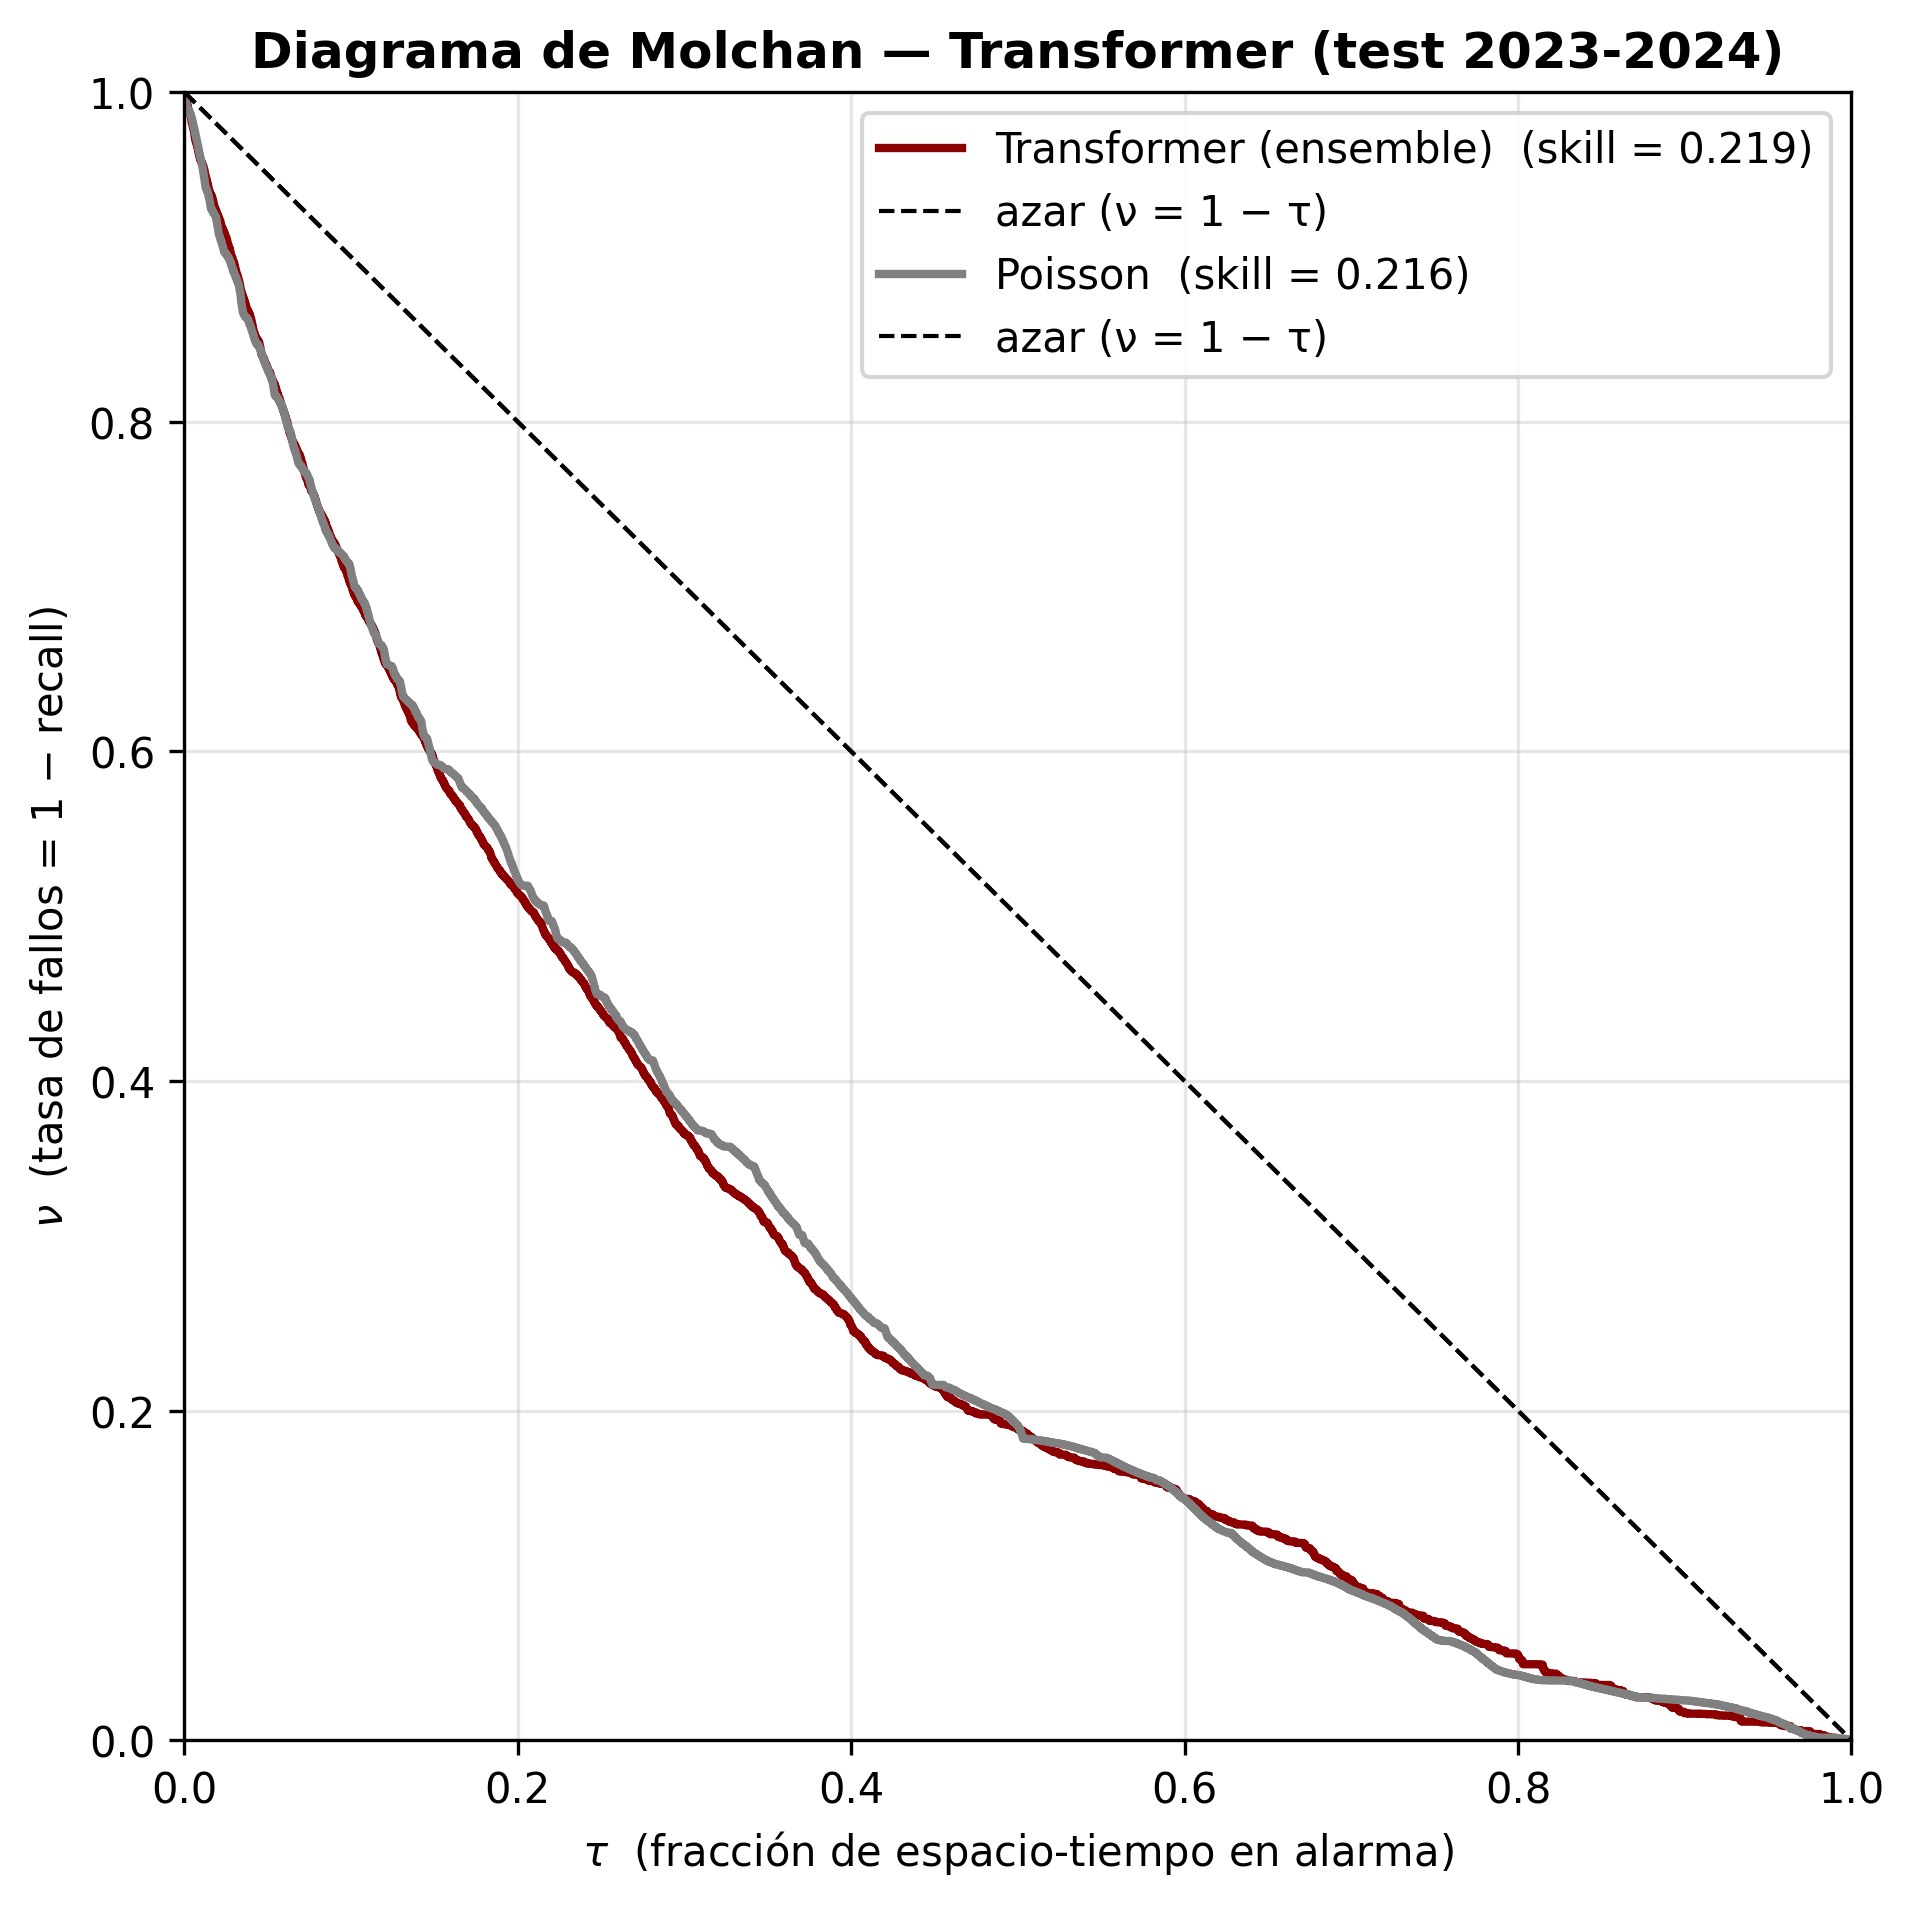
\includegraphics[width=0.62\textwidth]{figuras/05_molchan}
  \caption[Diagrama de Molchan del Transformer]{\textbf{Diagrama de Molchan} del Transformer frente al Poisson. La curva por debajo de la diagonal indica habilidad predictiva; el área entre la curva y la diagonal resume el \textit{skill} del pronosticador.}
  \label{fig:molchan}
\end{figure}

La proximidad entre las curvas del modelo y del Poisson es, en sí misma, un resultado
informativo: indica que buena parte de la capacidad del Transformer coincide con la que aporta
conocer la climatología sísmica. El análisis de la Sección~\ref{res-temporal} precisa de dónde
procede exactamente esta capacidad.

\subsection{Métricas operativas: el sistema como herramienta de alerta}
\label{res-operativas}

El AUC resume el rendimiento promediando sobre todos los umbrales de decisión, pero un sistema de
alerta real solo puede emitir un número limitado de avisos. Para evaluar el sistema desde esa
óptica se usan las métricas en el top \(K\): si se alerta del \(K\)\,\% de las ventanas con mayor
riesgo, ¿qué fracción de terremotos se captura y cuántas veces se mejora respecto al azar? La
Tabla~\ref{tab:operativas} recoge estas cifras para el Transformer y el Poisson, y la
Figura~\ref{fig:lift} las presenta de forma continua mediante la curva de \textit{lift}.

\begin{table}[ht!]
  \centering
  \small
  \begin{tabular}{@{}lcc@{}}
    \toprule
    \textbf{Métrica}          & \textbf{Transformer} & \textbf{Poisson} \\
    \midrule
    PR-AUC                    & 0.111                & 0.110            \\
    \textit{Precision} @1\,\% & 0.187                & 0.186            \\
    \textit{Recall} @1\,\%    & 0.042                & 0.041            \\
    \textit{Lift} @1\,\%      & \textbf{4.17}        & 4.14             \\
    \textit{Precision} @5\,\% & 0.150                & 0.151            \\
    \textit{Recall} @5\,\%    & 0.167                & 0.168            \\
    \textit{Lift} @5\,\%      & 3.35                 & 3.36             \\
    \bottomrule
  \end{tabular}
  \caption[Métricas operativas del Transformer frente al Poisson]{\textbf{Métricas operativas (top \(K\)).} \textit{Precision}, \textit{recall} y \textit{lift} al alertar del top \(K\)\,\% de mayor riesgo. El \textit{lift} indica cuántas veces se mejora respecto a una alerta aleatoria.}
  \label{tab:operativas}
\end{table}

\begin{figure}[ht!]
  \centering
  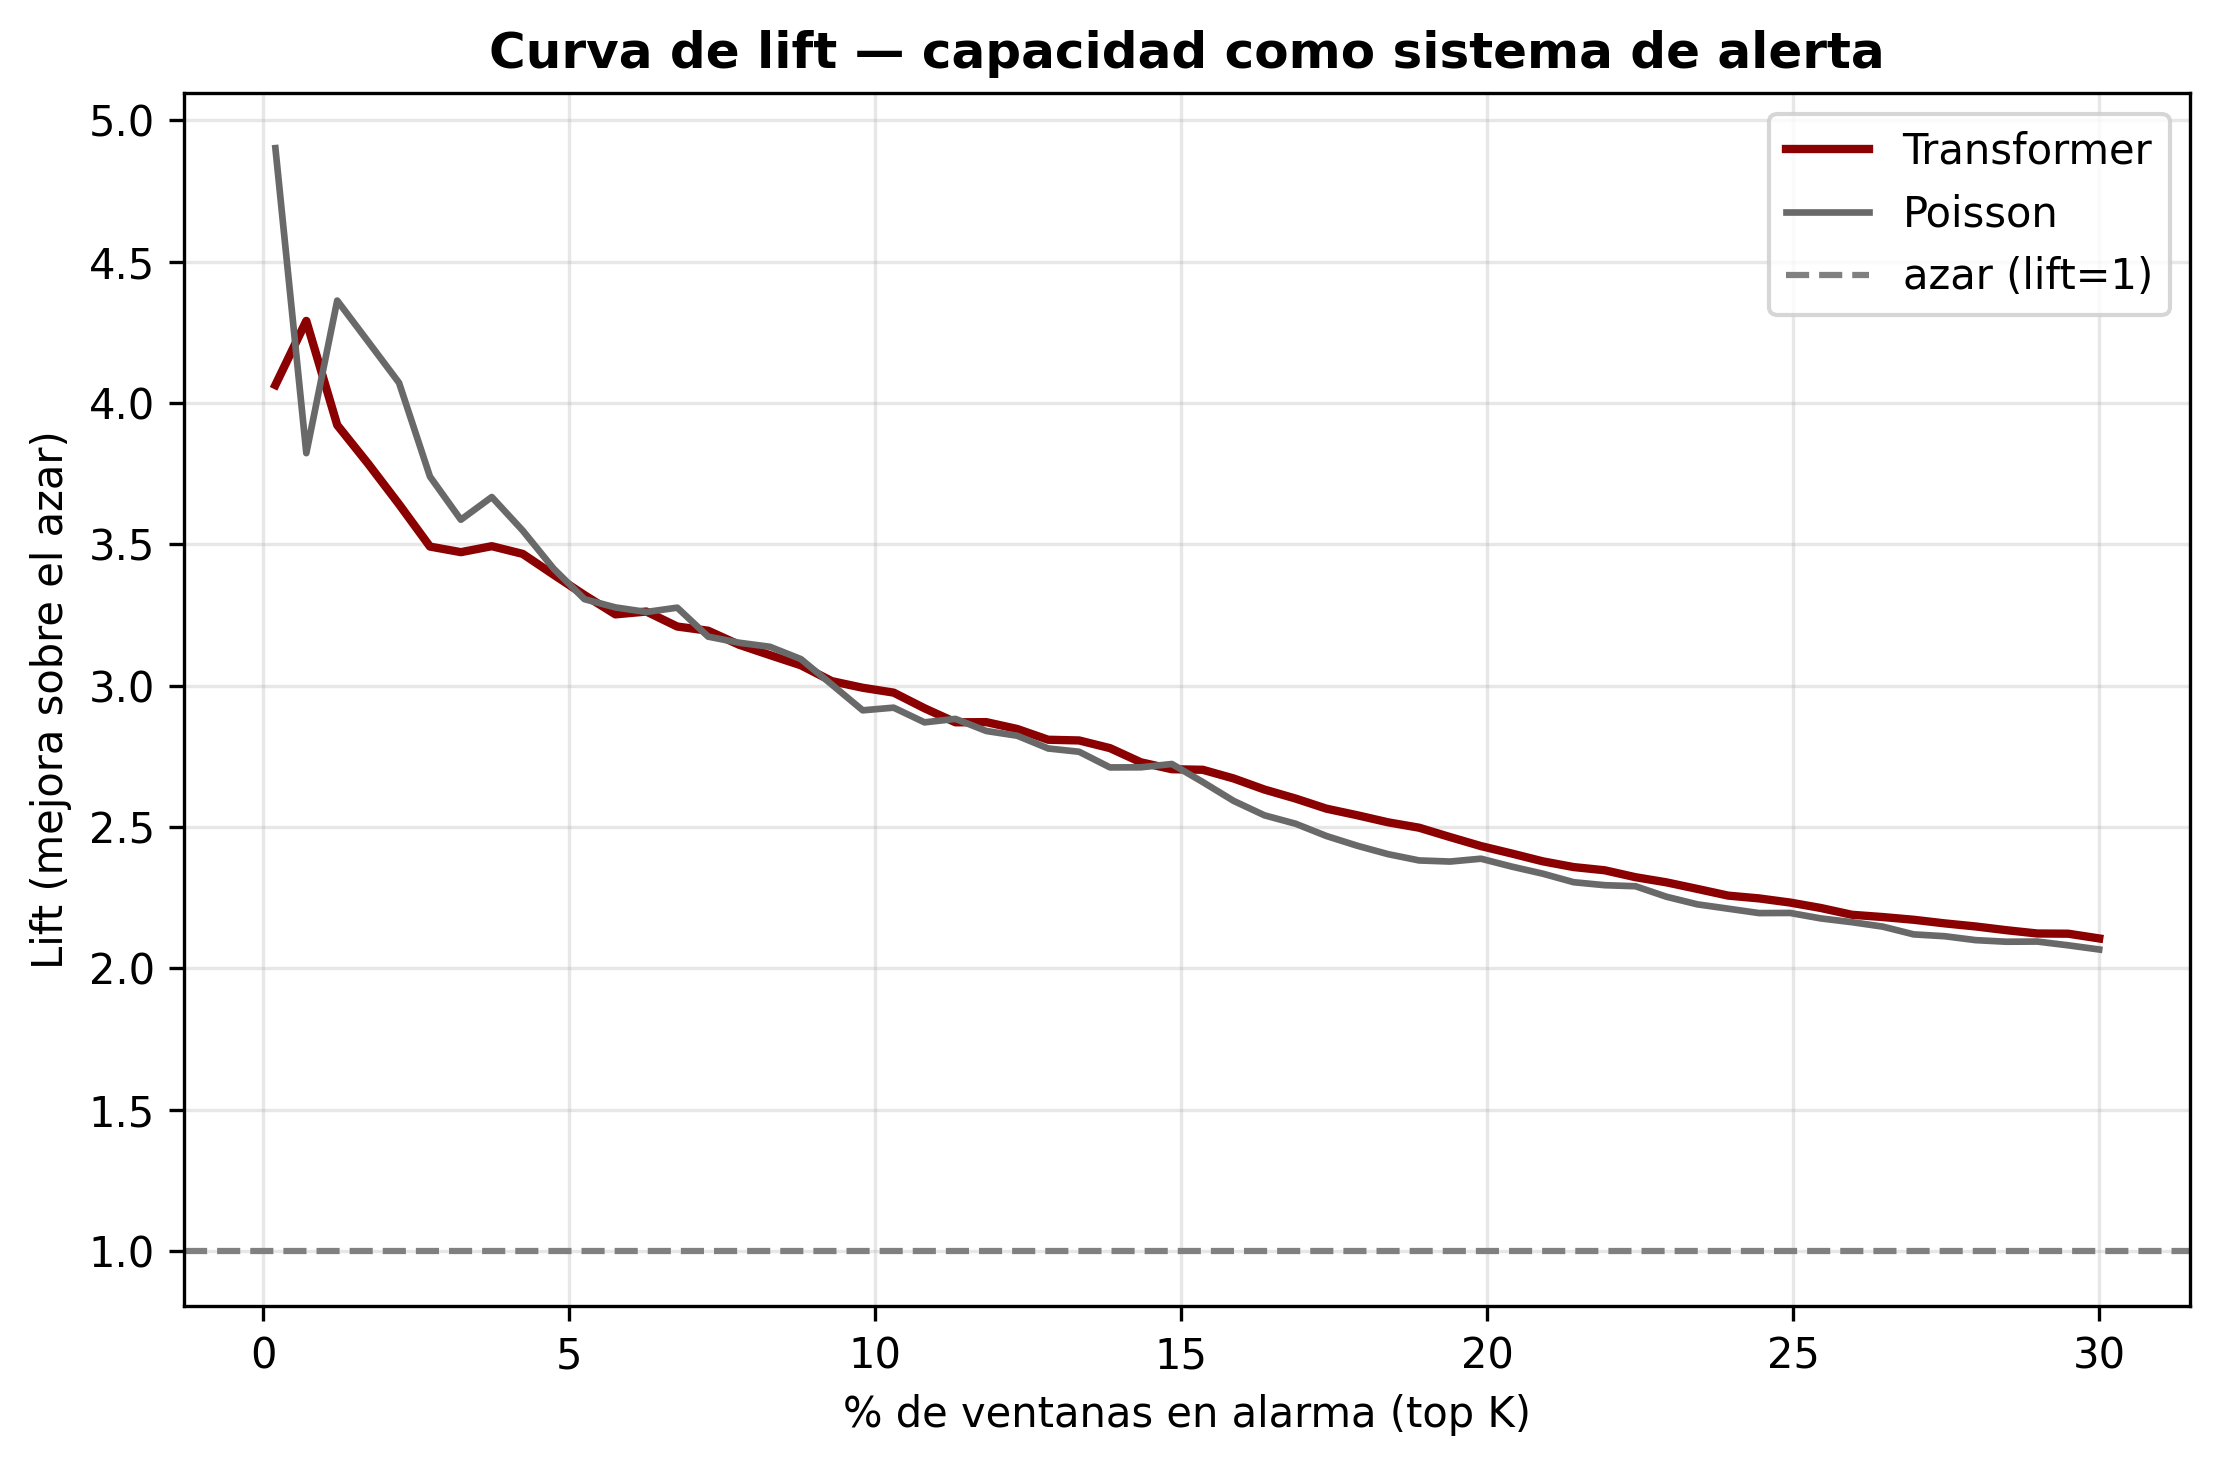
\includegraphics[width=0.74\textwidth]{figuras/05_lift_curve}
  \caption[Curva de \textit{lift} del Transformer]{\textbf{Curva de \textit{lift}.} Mejora respecto al azar al alertar del top \(K\)\,\% de mayor riesgo, en función de \(K\). Para alarmas muy concentradas (valores pequeños de \(K\)) la mejora supera cuatro veces el azar. Las curvas del Transformer y del Poisson son casi coincidentes.}
  \label{fig:lift}
\end{figure}

La lectura operativa es positiva: las alertas más confiadas del Transformer aciertan unas
\textbf{cuatro veces más que el azar} (\textit{lift} de 4.17 en el top 1\,\%). Concentrando las
alarmas en las zonas que el modelo considera más peligrosas se multiplica por cuatro la
probabilidad de acertar. La Figura~\ref{fig:pr} complementa este análisis con la curva
\textit{precision}-\textit{recall}, más adecuada que la ROC en un problema tan desbalanceado.
Estas cifras son prácticamente idénticas a las del Poisson, lo que vuelve a señalar que la
capacidad del sistema proviene de la cartografía espacial del peligro.

\begin{figure}[ht!]
  \centering
  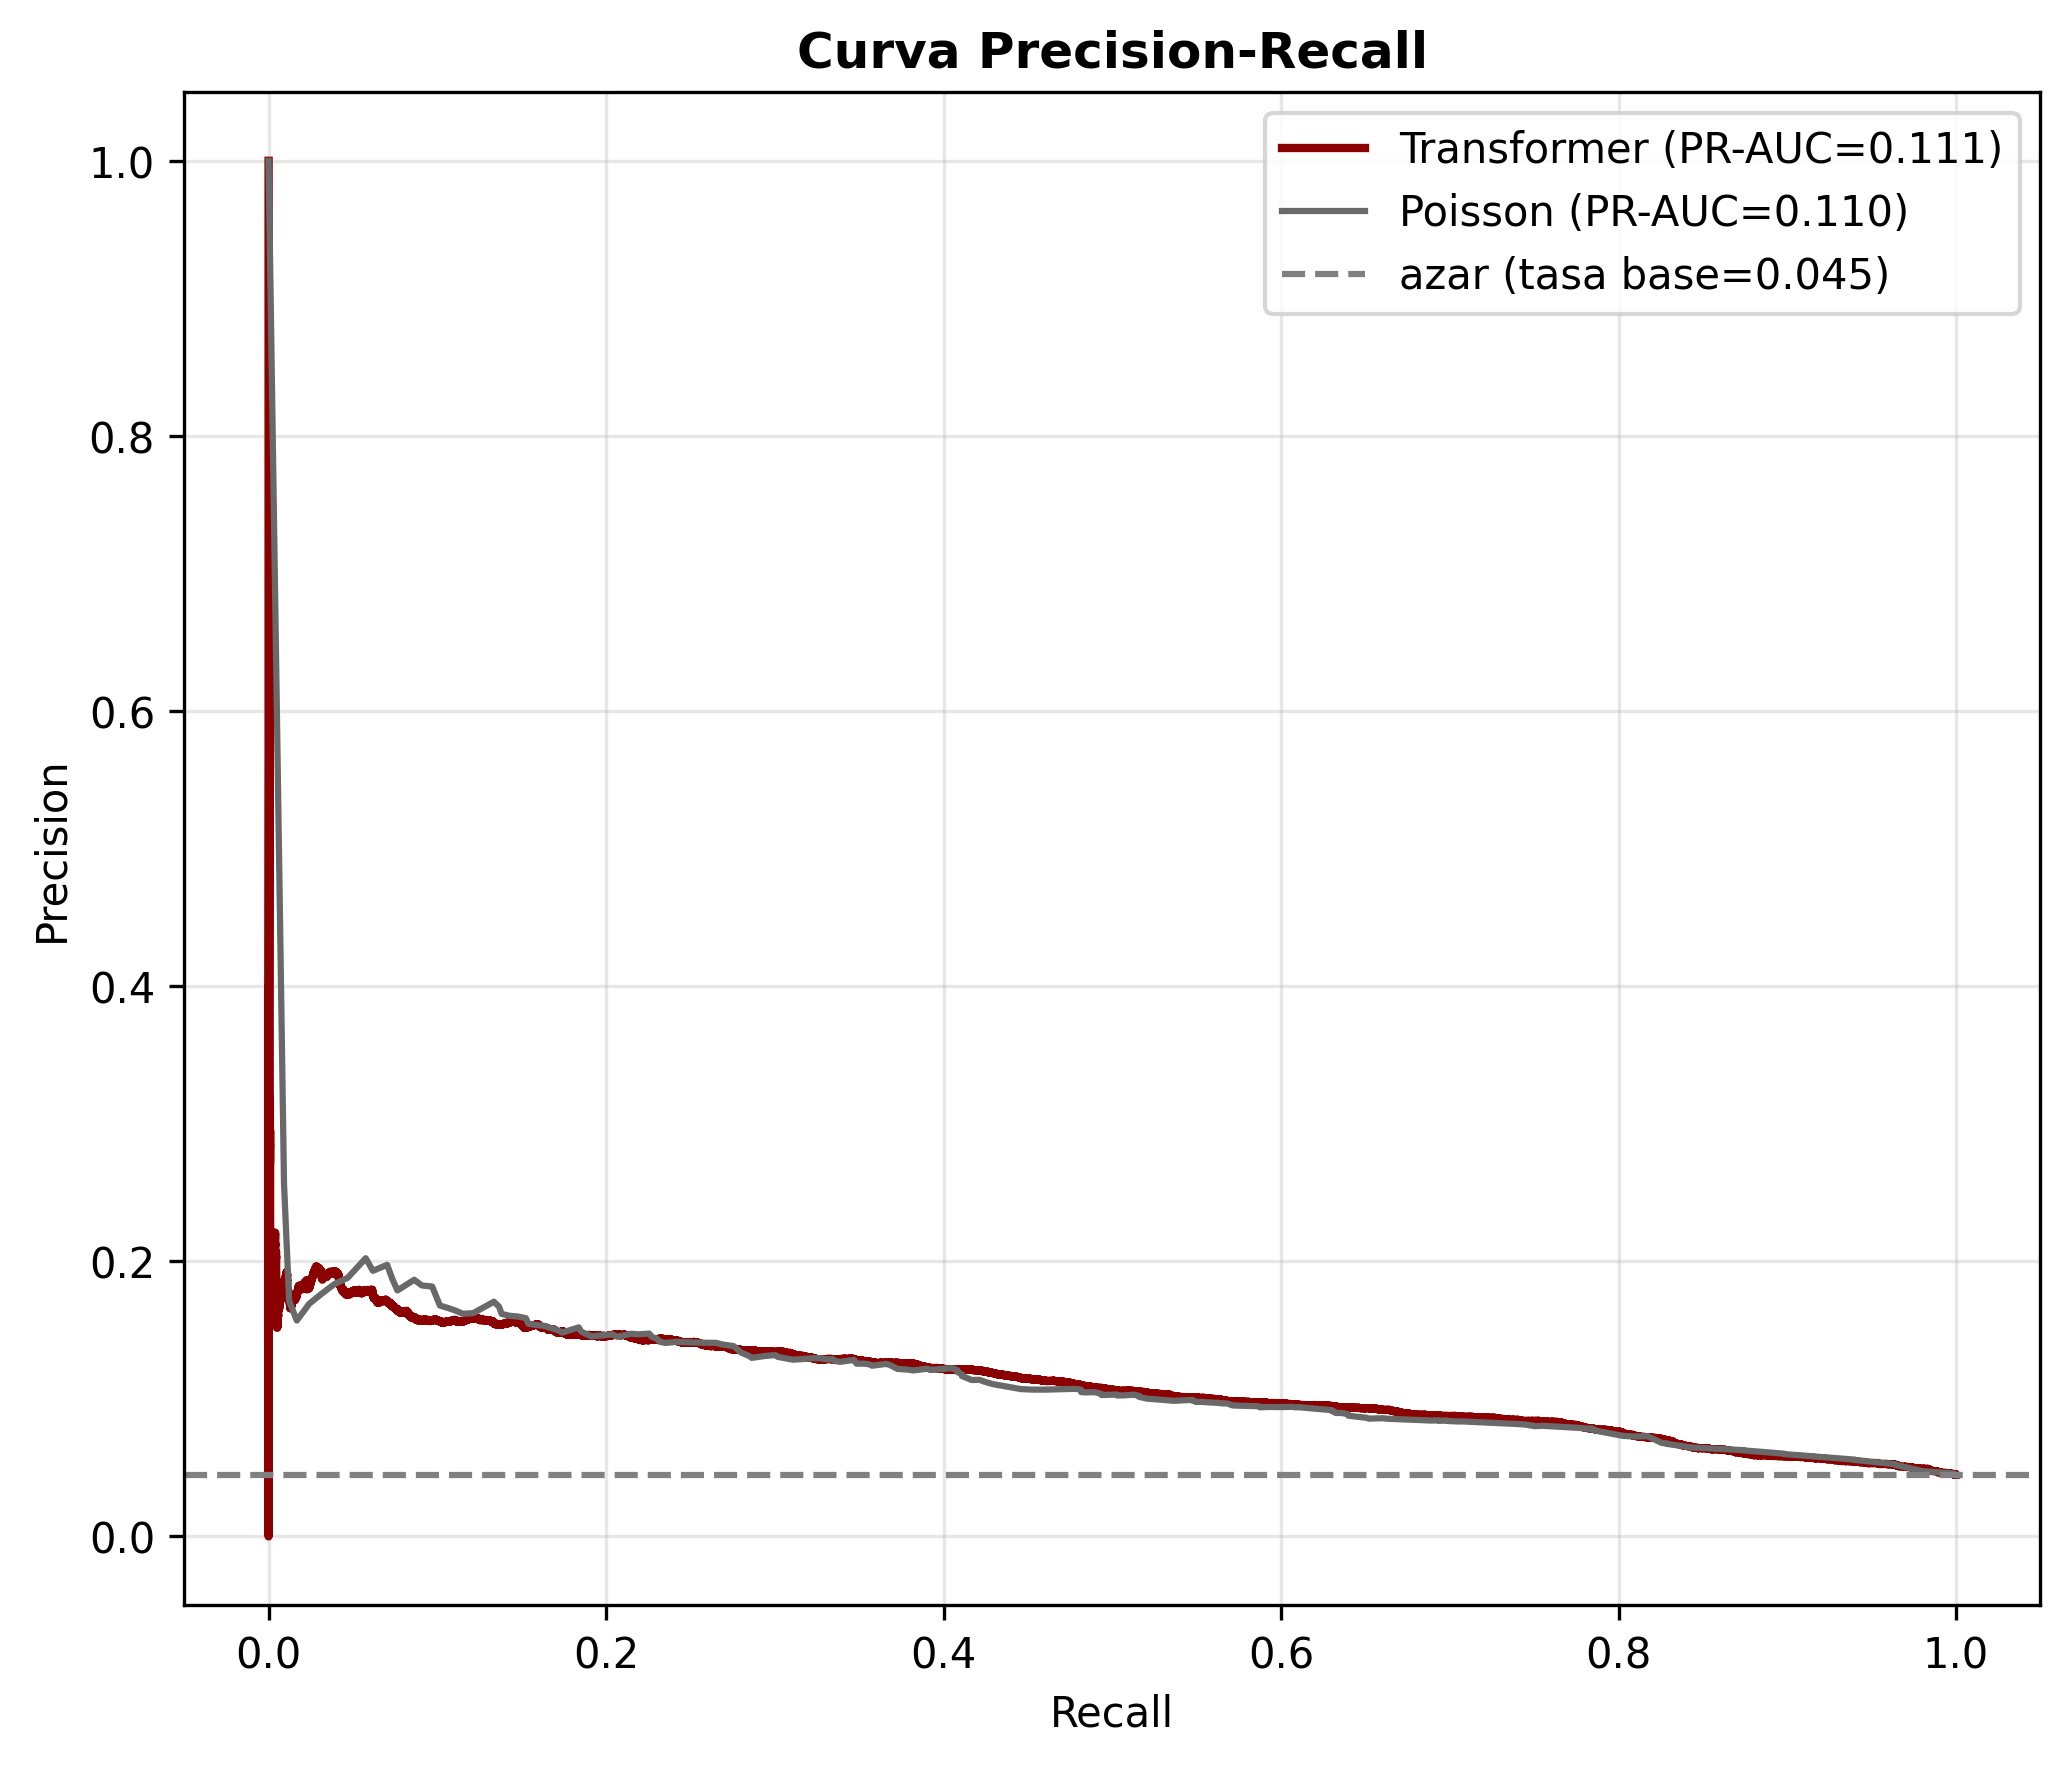
\includegraphics[width=0.66\textwidth]{figuras/05_pr_curve}
  \caption[Curva \textit{precision}-\textit{recall} del Transformer]{\textbf{Curva \textit{precision}-\textit{recall}} del Transformer frente al Poisson. La línea discontinua marca la tasa base, que es el nivel de un modelo aleatorio en esta métrica.}
  \label{fig:pr}
\end{figure}

Otra forma de comprobar que el modelo capta señal es observar cómo reparte sus probabilidades
entre los casos positivos y negativos. La Figura~\ref{fig:scoredist} superpone los dos
histogramas: el de las probabilidades asignadas a las ventanas que sí tuvieron un mainshock y el
de las que no. Aunque las dos distribuciones se solapan en gran medida --algo esperable en un
problema tan difícil y desbalanceado--, la distribución de los positivos está claramente
desplazada hacia probabilidades más altas, con una media mayor que la de los negativos. Es decir,
el modelo no asigna riesgo al azar: tiende a otorgar valores más elevados precisamente a las
ventanas que acaban siendo positivas, que es exactamente lo que sustenta el \textit{lift} y la
capacidad de alerta descritos arriba. El solapamiento, lejos de ser un defecto del modelo, refleja
la dificultad intrínseca del problema.

\begin{figure}[ht!]
  \centering
  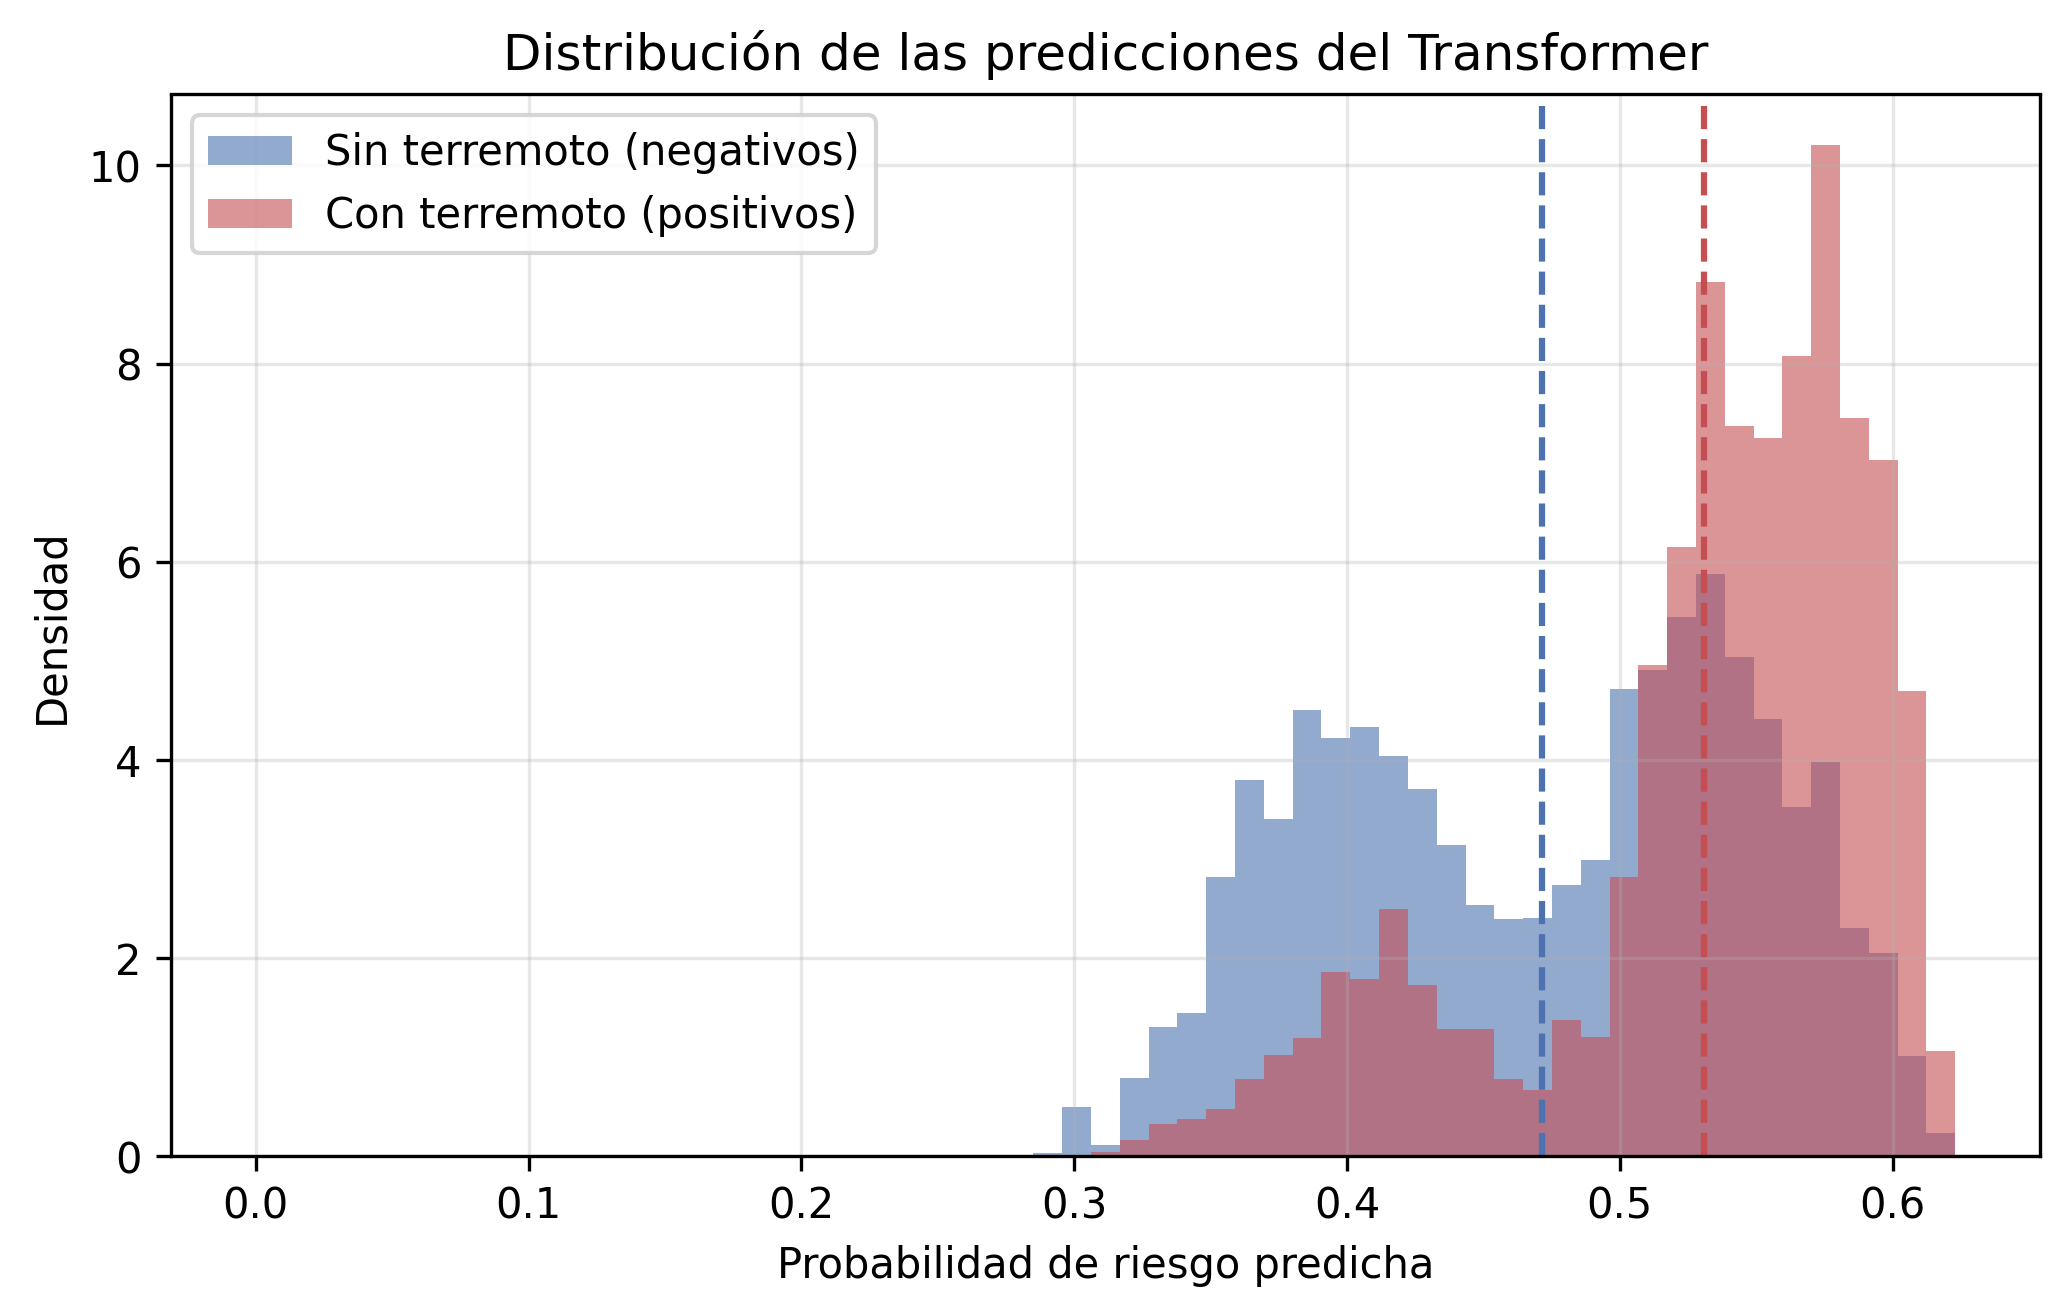
\includegraphics[width=0.72\textwidth]{figuras/05_score_dist}
  \caption[Distribución de las probabilidades predichas]{\textbf{Distribución de las probabilidades predichas por el Transformer}, separadas según el resultado real (con o sin mainshock). Las líneas discontinuas marcan las medias de cada grupo. La distribución de los positivos está desplazada hacia valores más altos, lo que muestra que el modelo concentra el riesgo en las ventanas correctas.}
  \label{fig:scoredist}
\end{figure}

\subsection{Análisis de la dimensión espacial y temporal}
\label{res-temporal}

El AUC global de 0.73 mezcla dos contribuciones de naturaleza muy distinta. Para separarlas se
recurre a la AUC temporal por celda, introducida en la Sección~\ref{md-metricas}. La idea es
preguntar, dentro de cada celda por separado, si el modelo distingue las ventanas de 30 días que
tendrán un terremoto de las que no. Un modelo que solo conociera la tasa media de cada celda
--como el Poisson-- obtendría exactamente 0.5 en esta métrica, porque asigna el mismo valor a
todas las ventanas de una misma celda.

La Figura~\ref{fig:auctemporal} muestra la distribución de la AUC temporal por celda para el
Transformer. La media se sitúa en torno a 0.50, prácticamente idéntica a la del Poisson. Esto
delimita con precisión dónde reside la información que aprovecha el sistema: \textbf{la capacidad
  discriminativa procede de la dimensión espacial} --es decir, de saber qué celdas son crónicamente
más activas-- mientras que la componente temporal a 30 días, una vez aislada, no añade
información por encima de la tasa base.

\begin{figure}[ht!]
  \centering
  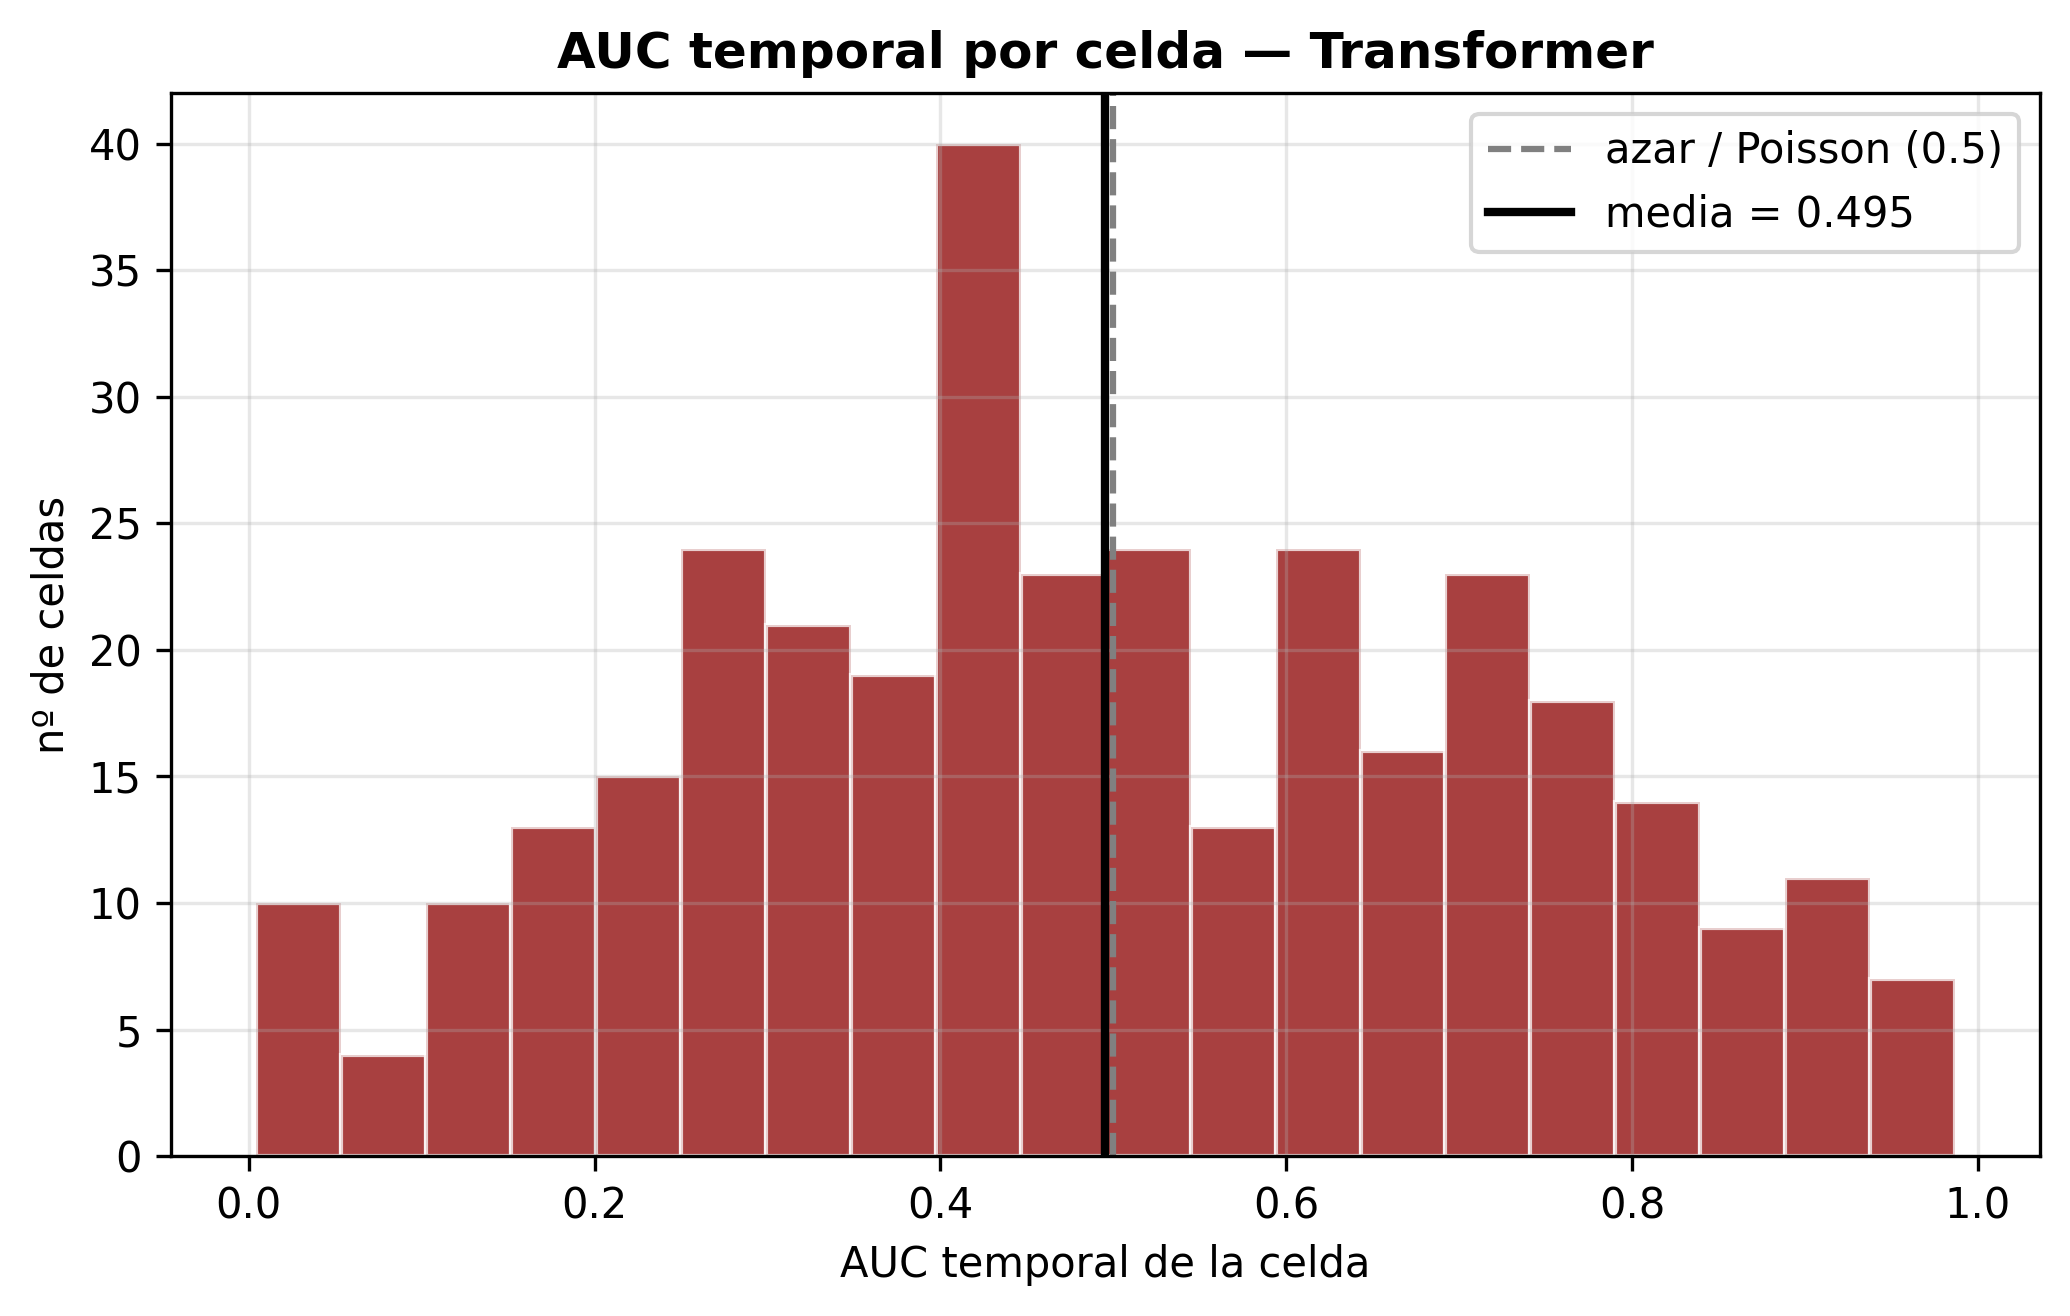
\includegraphics[width=0.74\textwidth]{figuras/05_auc_temporal}
  \caption[Distribución de la AUC temporal por celda]{\textbf{AUC temporal por celda} del Transformer. Cada barra cuenta las celdas con un valor dado. La media se sitúa cerca de 0.5, lo que indica que la capacidad de ordenar las ventanas temporales dentro de cada celda coincide con la de la climatología.}
  \label{fig:auctemporal}
\end{figure}

Este resultado es coherente con el consenso de la comunidad sismológica y constituye una de las
aportaciones del trabajo: gracias a una métrica diseñada específicamente, se localiza con
precisión la información predictiva. El sistema responde muy bien a la pregunta de \emph{dónde} es
más probable un terremoto --la estructura espacial de la sismicidad es estable y aprendible--
mientras que la pregunta de \emph{cuándo}, en un horizonte de 30 días y sobre el catálogo de
eventos, no encuentra una respuesta estadísticamente sólida. Esta distinción, lejos de ser una
limitación del método, es un hallazgo: indica que el valor del sistema está en la cartografía de
peligro espacial, que es justo lo que aprovecha la última fase.

Este mismo patrón se observa en la red de grafos, lo que confirma que no es una particularidad
del Transformer sino una propiedad del problema. La Figura~\ref{fig:gnncomp} reúne las curvas ROC
y de Molchan de la GNN frente al Poisson y la distribución de su AUC temporal por celda. Las dos
primeras muestran un comportamiento muy parecido al del Transformer, y la tercera vuelve a
situarse en torno a 0.5. Es decir, ambos modelos espaciales coinciden tanto en lo que logran
(cartografía espacial) como en lo que no (anticipación temporal), lo que da solidez a la
conclusión.

\begin{figure}[ht!]
  \centering
  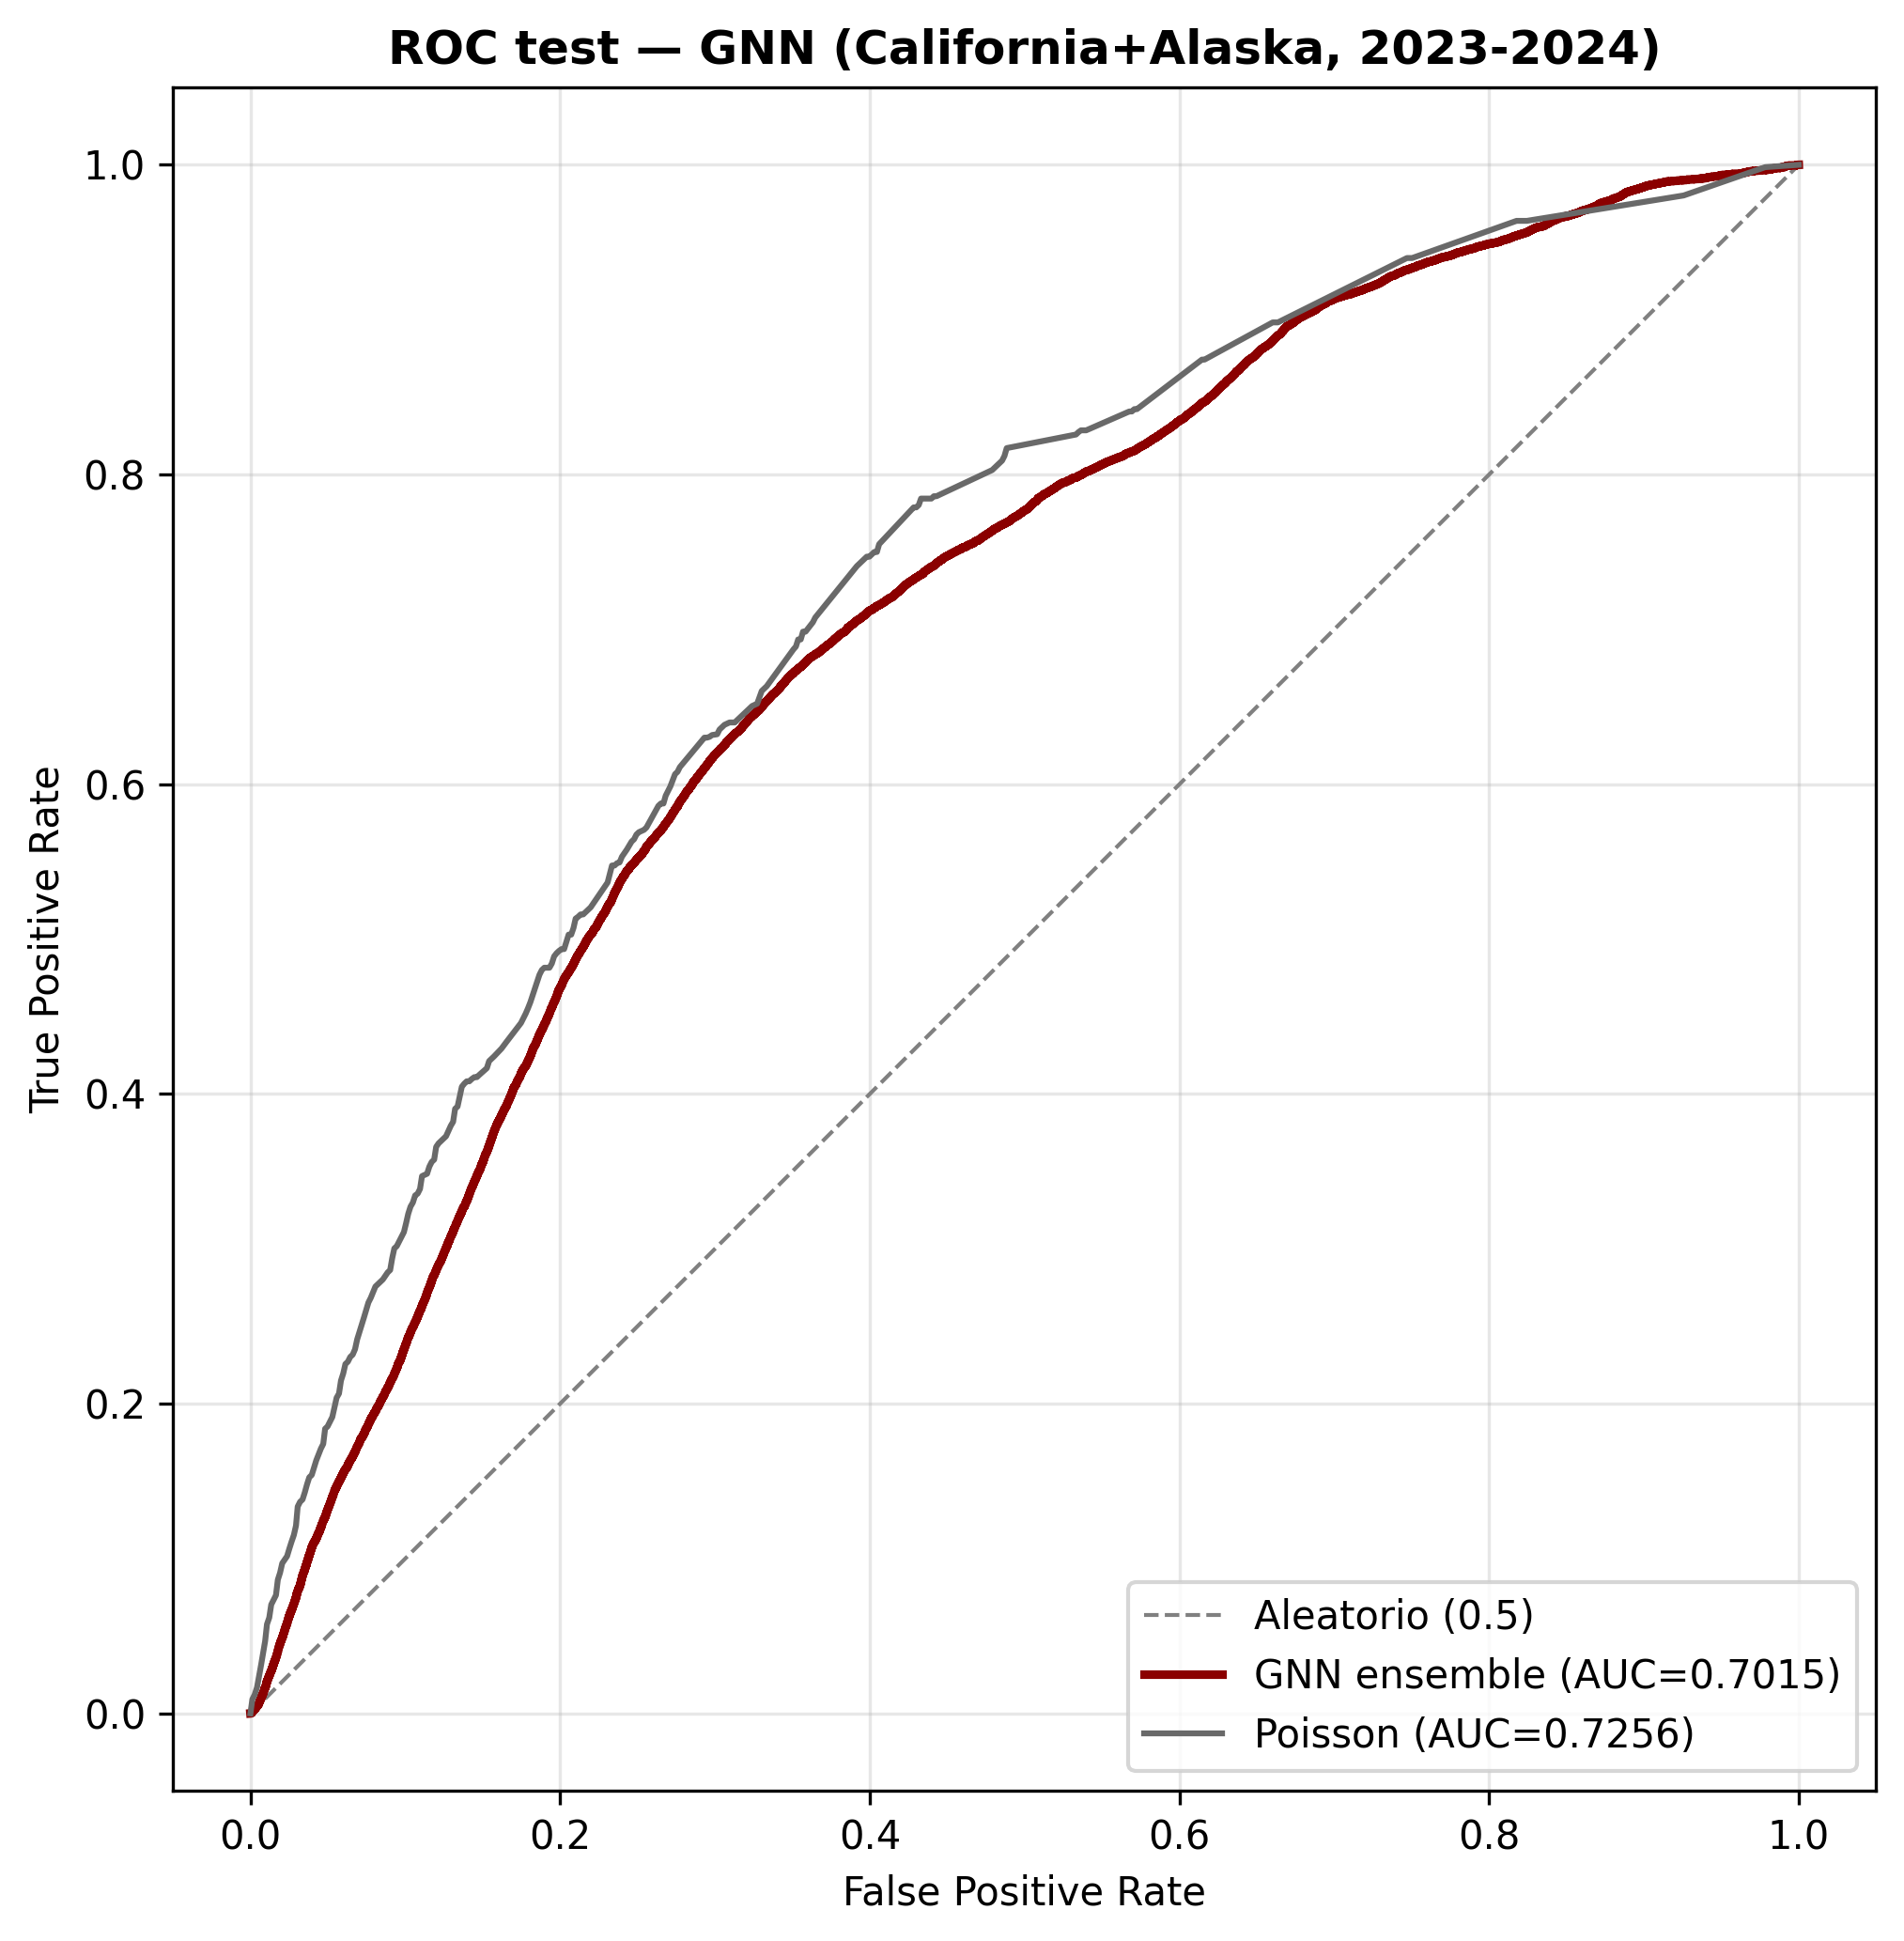
\includegraphics[width=0.49\textwidth]{figuras/04_roc_test}
  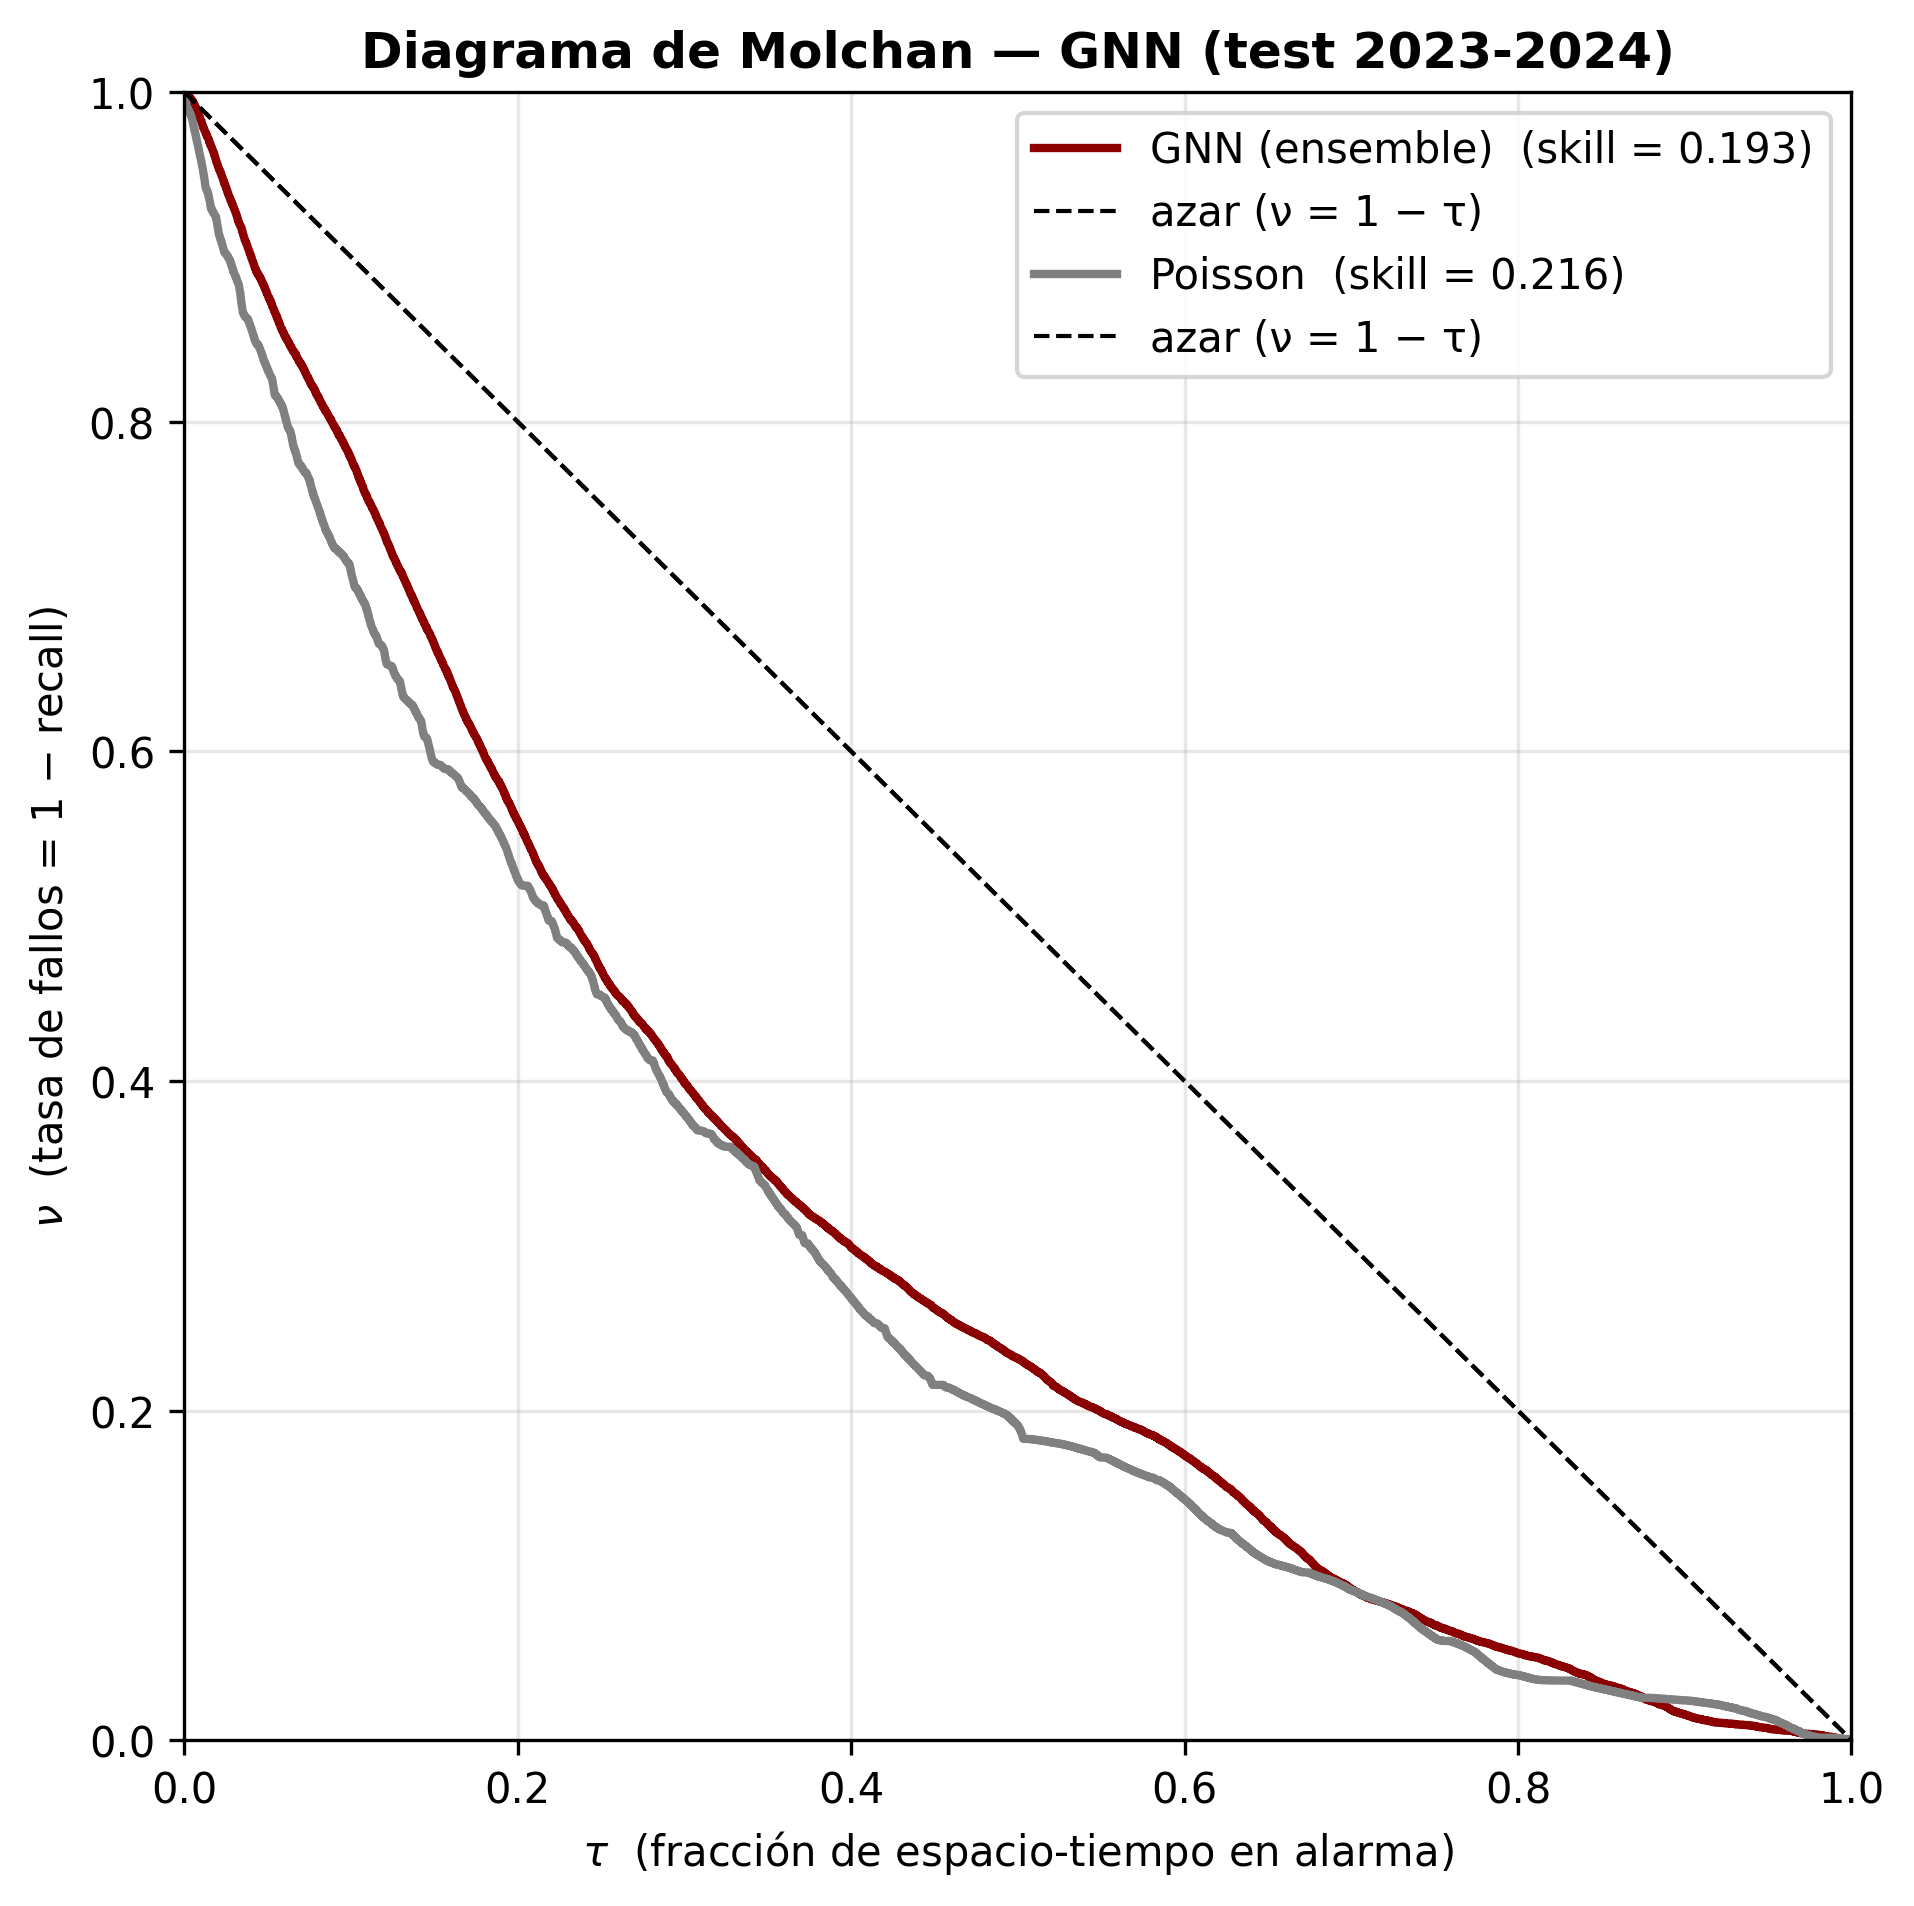
\includegraphics[width=0.49\textwidth]{figuras/04_molchan}\\[0.3cm]
  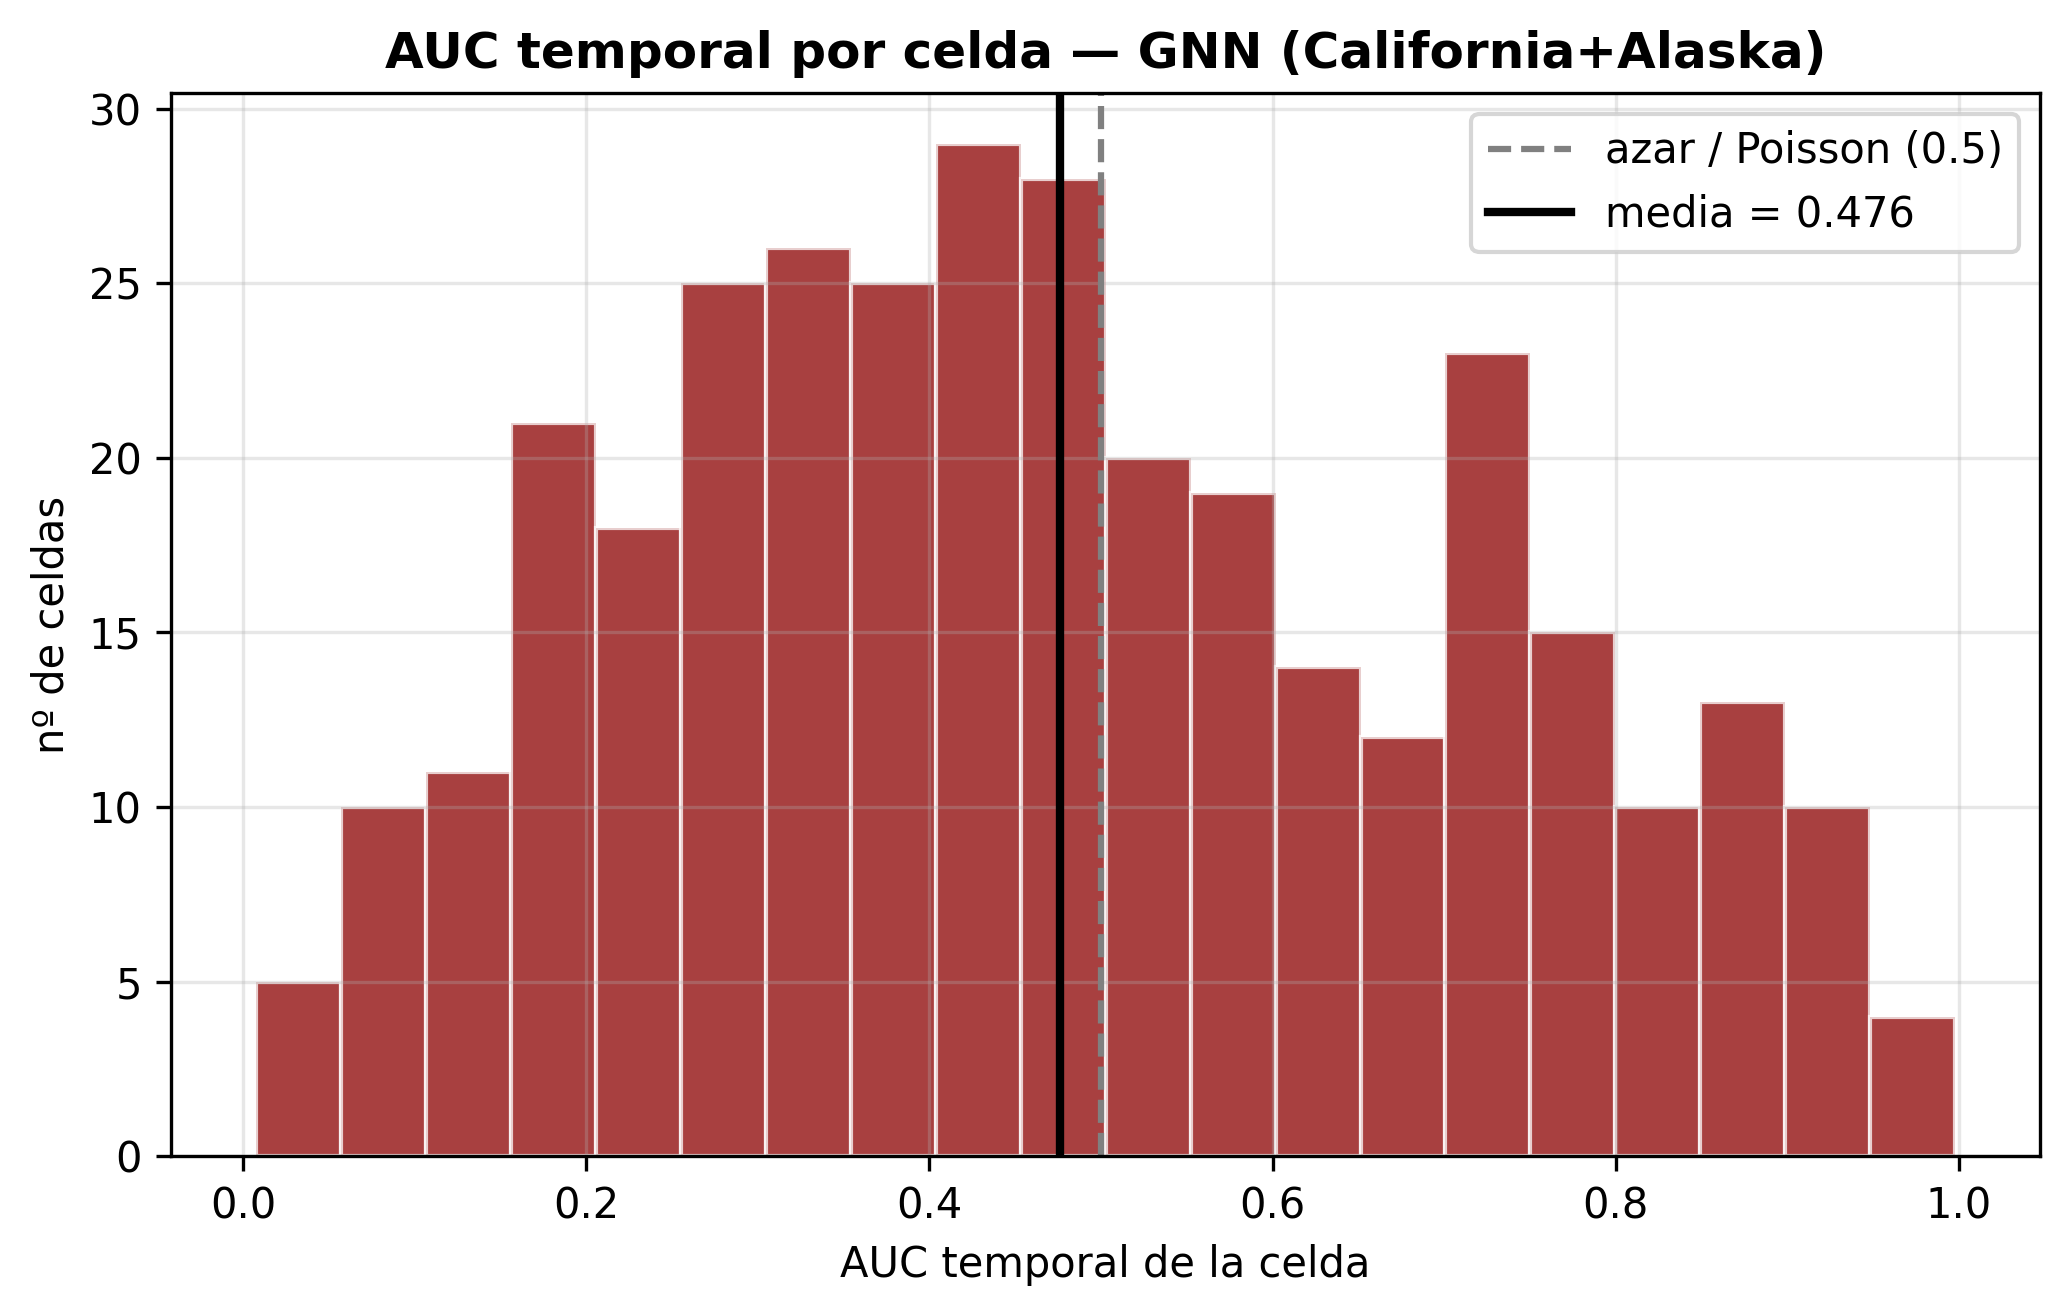
\includegraphics[width=0.6\textwidth]{figuras/04_auc_temporal}
  \caption[Resultados de la red de grafos]{\textbf{Resultados de la red de grafos (GNN).} Arriba: curva ROC (izquierda) y diagrama de Molchan (derecha) frente al Poisson. Abajo: distribución de la AUC temporal por celda, de nuevo centrada en torno a 0.5. El comportamiento reproduce el del Transformer, lo que confirma que este resultado se debe a la naturaleza del problema y no al tipo de arquitectura empleada.}
  \label{fig:gnncomp}
\end{figure}

\subsection{Estudios de ablación}
\label{res-ablations}

Para entender qué decisiones de diseño influyen en el resultado, y con qué dirección, se
realizaron varios estudios de ablación. La Tabla~\ref{tab:ablations} los resume. Cada uno
modifica un único elemento respecto al modelo de referencia y observa su efecto, prestando
especial atención a la AUC temporal por celda, que es la métrica que mide la señal predictiva
real.

Dos resultados de la tabla merecen comentario. Primero, al eliminar el \textit{declustering} el
AUC global sube, pero la AUC temporal por celda permanece en 0.509, prácticamente en el azar: la
mejora se explica íntegramente por la predictibilidad trivial de las réplicas, no por una
capacidad precursora nueva, lo que confirma que la decisión de declusterizar es metodológicamente
necesaria. Segundo, la adición de características diseñadas específicamente para captar anomalías
temporales por celda tampoco mejora el rendimiento del modelo. En conjunto, los estudios de ablación muestran que la conclusión
sobre la dimensión temporal es \textbf{robusta}: se mantiene al cambiar la arquitectura, la
ventana, el preprocesado del catálogo y las características. Esta robustez refuerza el valor del
hallazgo, porque descarta que se deba a una elección concreta de diseño.

\begin{table}[ht!]
  \centering
  \small
  \begin{tabular}{@{}lll@{}}
    \toprule
    \textbf{Variación}                    & \textbf{Efecto observado}               & \textbf{AUC temporal} \\
    \midrule
    Arquitectura GCN \(\to\) GAT          & mejora marginal, sin salto cualitativo  & 0.476                 \\
    \textit{Pooling} temporal completo    & ligera mejora del AUC global            & 0.495                 \\
    Ventana 30\,d \(\to\) 14\,d           & empeora el AUC global                   & 0.501                 \\
    Catálogo sin \textit{declustering}    & sube el AUC global (réplicas triviales) & 0.509                 \\
    Características de anomalía por celda & sin mejora apreciable                   & 0.483                 \\
    Filtro de profundidad \(\leq 70\)\,km & ligera bajada del AUC global            & 0.463                 \\
    \bottomrule
  \end{tabular}
  \caption[Resumen de los estudios de ablación]{\textbf{Estudios de ablación.} Cada fila modifica un elemento del modelo. La AUC temporal por celda se mantiene en el entorno de 0.5 (entre 0.46 y 0.51) en todas las ablaciones medidas, lo que indica que la conclusión sobre la dimensión temporal es robusta frente a estas variaciones.}
  \label{tab:ablations}
\end{table}

\subsection{Calibración y mapas de riesgo}
\label{res-gp}

La última fase transforma las predicciones espaciales en mapas de riesgo. Antes de la
interpolación es necesario calibrar las probabilidades del modelo, porque la ponderación de clase
usada en el entrenamiento las infla. La Figura~\ref{fig:calibracion} muestra la curva de
fiabilidad antes y después de la calibración isotónica, validada sobre una mitad del test
independiente de la usada para ajustar la calibración, de modo que la comparación no es
circular. El \textit{Brier score} mejora de 0.28 a 0.09, una reducción de dos tercios: tras
la calibración, las probabilidades del mapa reflejan frecuencias de ocurrencia reales, lo que es
esencial para un producto orientado a la toma de decisiones, ya que un mapa que sobreestimara el
riesgo generaría fatiga de alarma.

\begin{figure}[ht!]
  \centering
  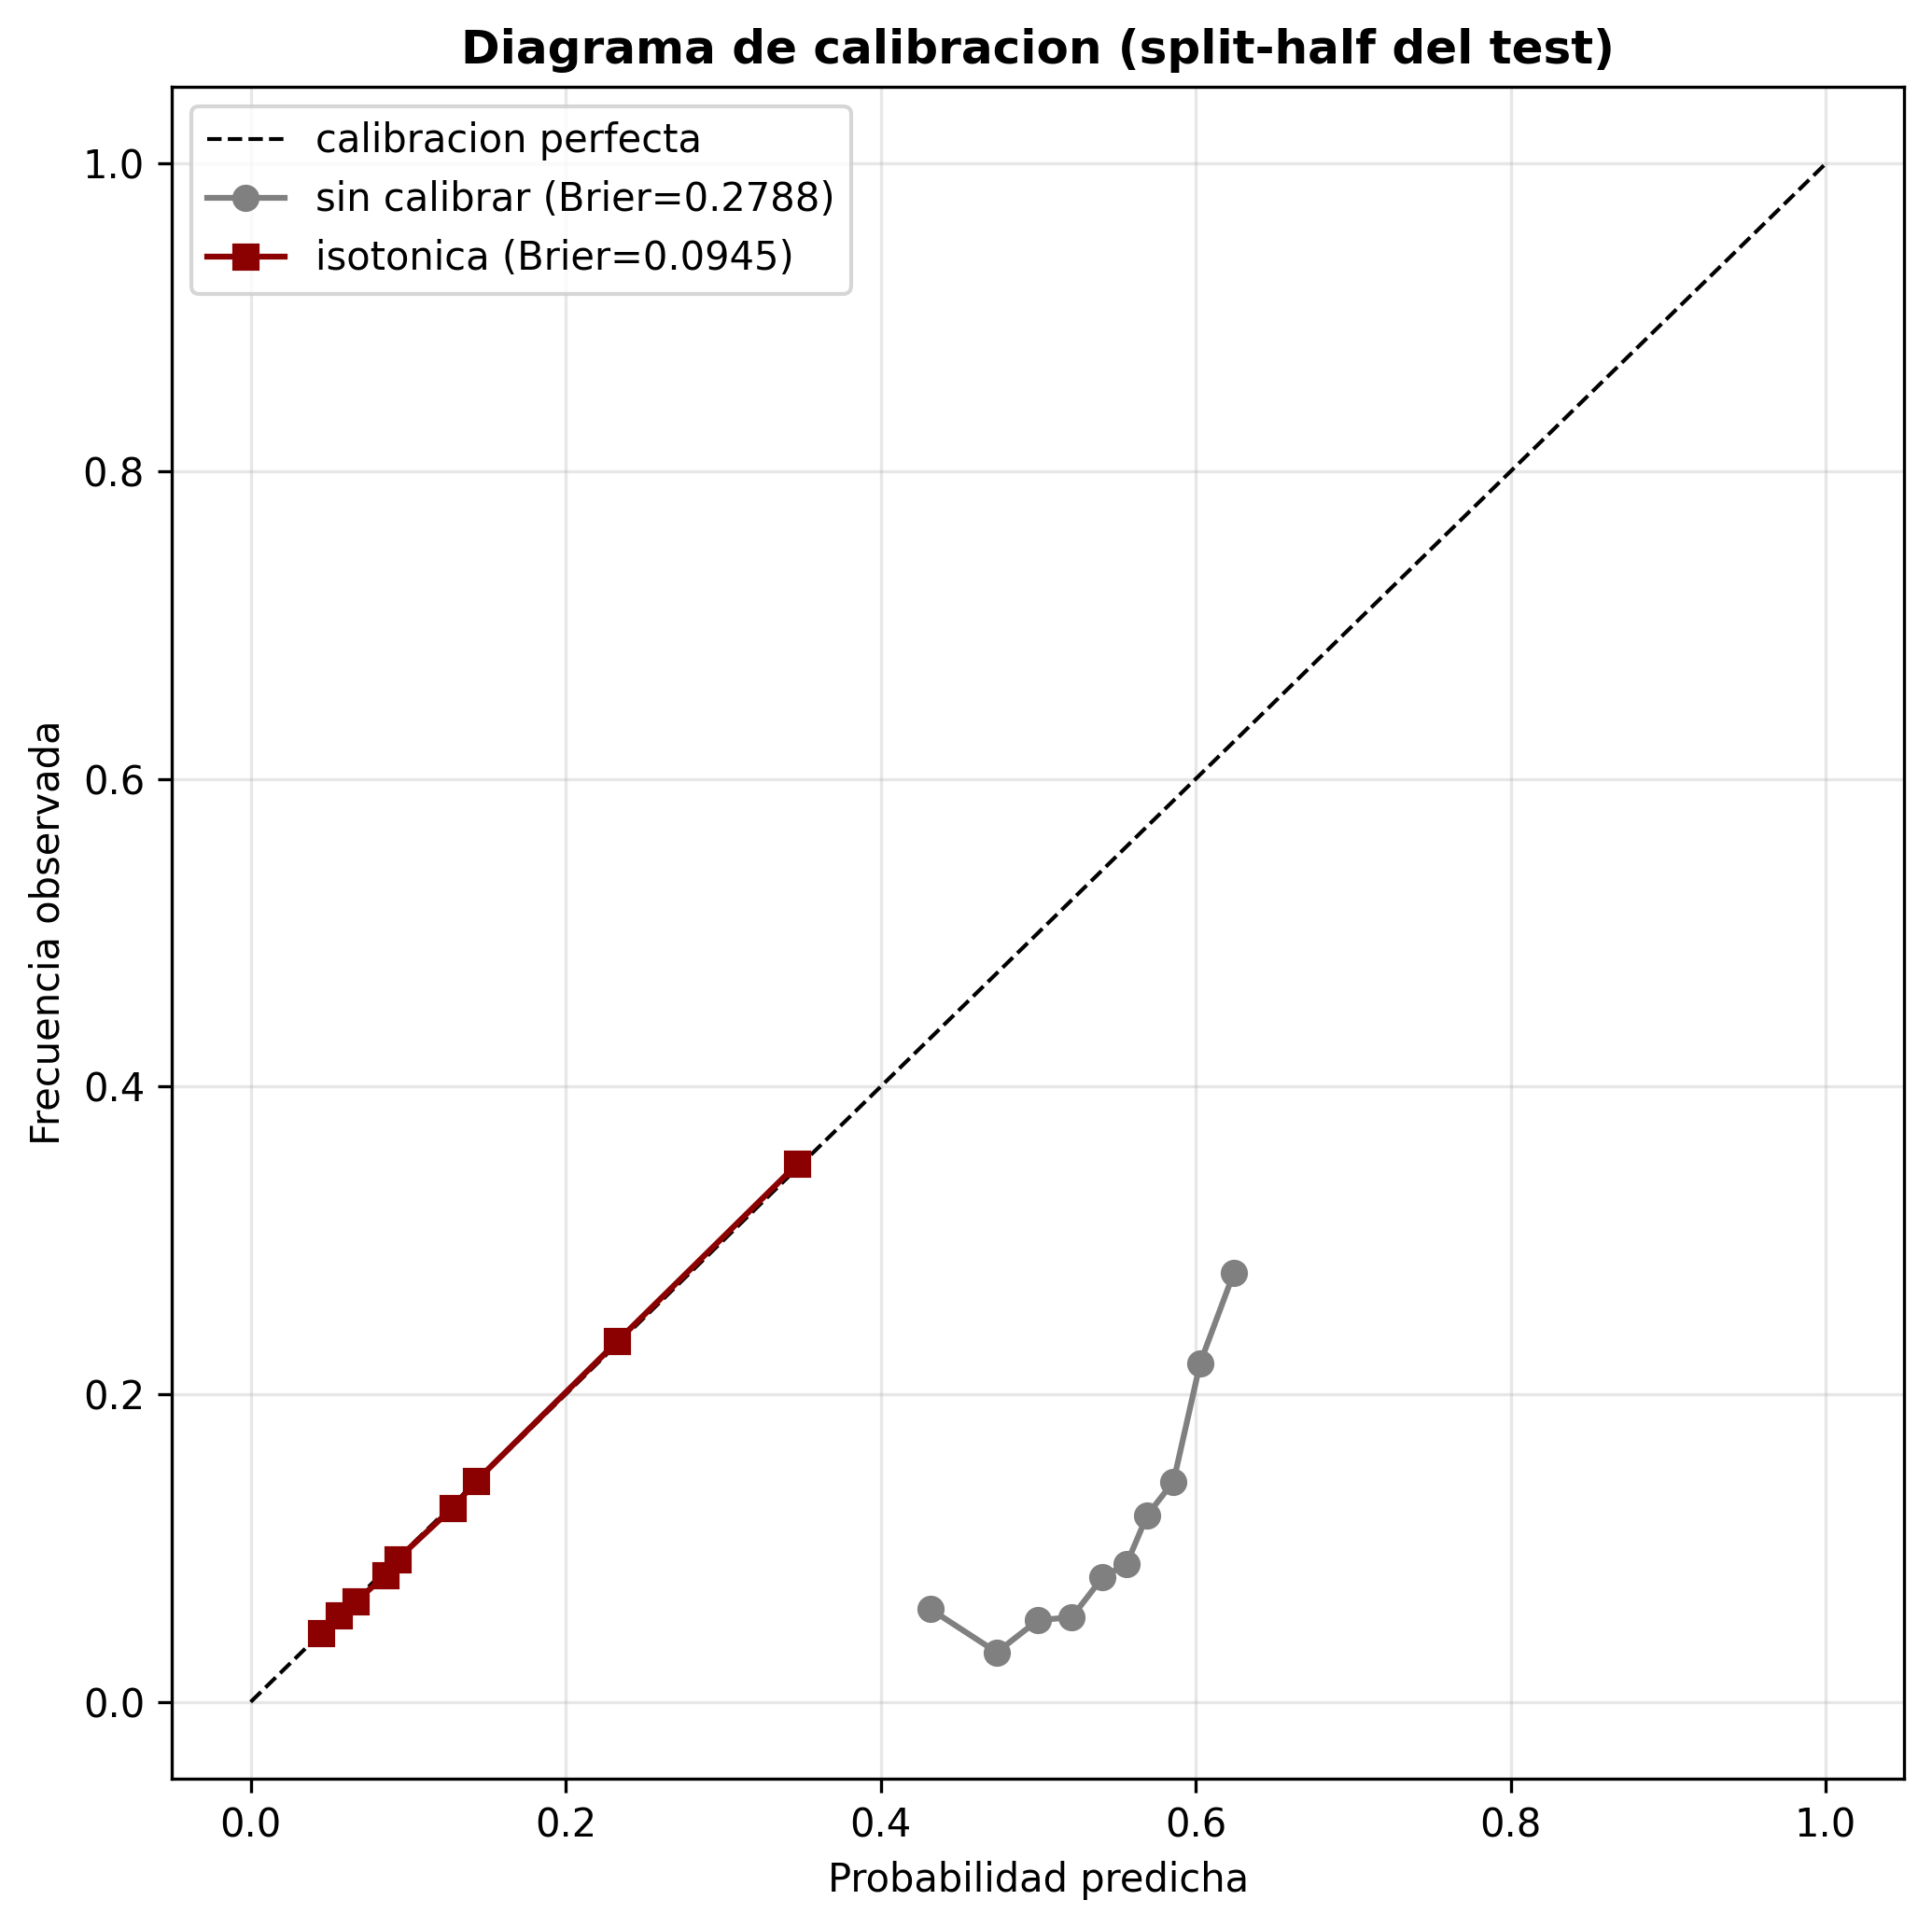
\includegraphics[width=0.6\textwidth]{figuras/06_calibracion}
  \caption[Curva de calibración y \textit{Brier score}]{\textbf{Diagrama de calibración.} Probabilidad predicha frente a frecuencia observada, antes (gris) y después (rojo) de la calibración isotónica. La calibración acerca las predicciones a la diagonal ideal y reduce el \textit{Brier score} de 0.28 a 0.09.}
  \label{fig:calibracion}
\end{figure}

Las Figuras~\ref{fig:mapacali} y~\ref{fig:mapaalaska} presentan los mapas de riesgo y de
incertidumbre obtenidos con el proceso gaussiano para California y Alaska. El mapa de riesgo
(izquierda) muestra una superficie continua que concentra el riesgo a lo largo de las grandes
estructuras tectónicas. El mapa de incertidumbre (derecha) es bajo cerca de las celdas con datos
y crece en las zonas sin sismicidad registrada, donde el modelo extrapola; es decir, la confianza
del mapa sigue a la disponibilidad de datos, como cabe esperar de un método bayesiano. Las
estrellas marcan los mainshocks reales del periodo de test, que tienden a caer en las zonas de
riesgo alto.

\begin{figure}[ht!]
  \centering
  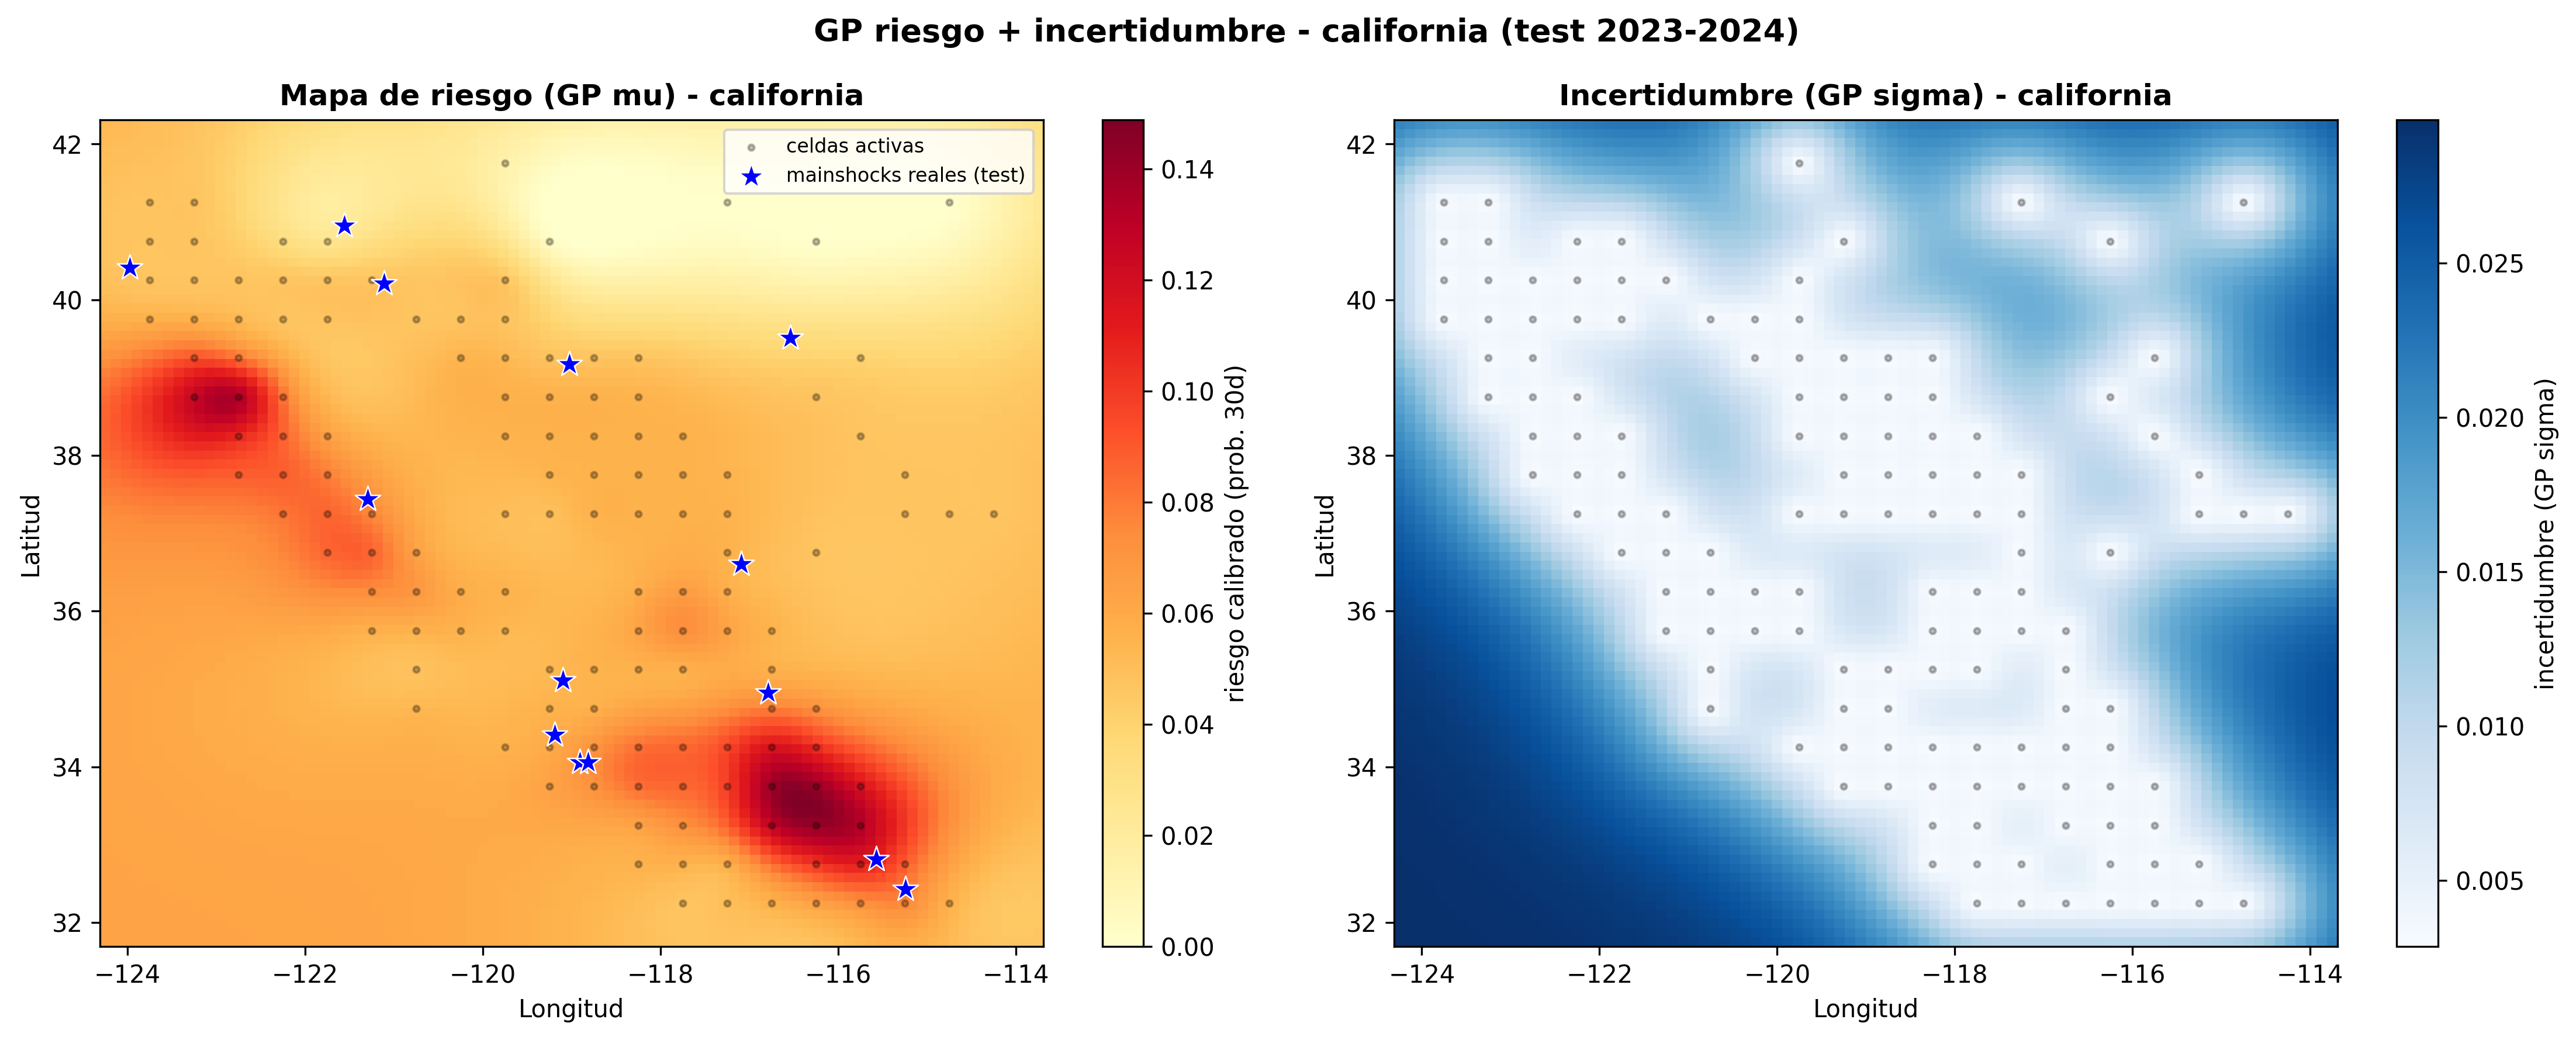
\includegraphics[width=\textwidth]{figuras/06_mapa_riesgo_gp_california}
  \caption[Mapa de riesgo e incertidumbre para California]{\textbf{Mapa de riesgo (izquierda) e incertidumbre (derecha) para California.} El riesgo se concentra a lo largo de la falla de San Andrés y sus ramales. Las estrellas marcan los mainshocks reales del periodo de test.}
  \label{fig:mapacali}
\end{figure}

\begin{figure}[ht!]
  \centering
  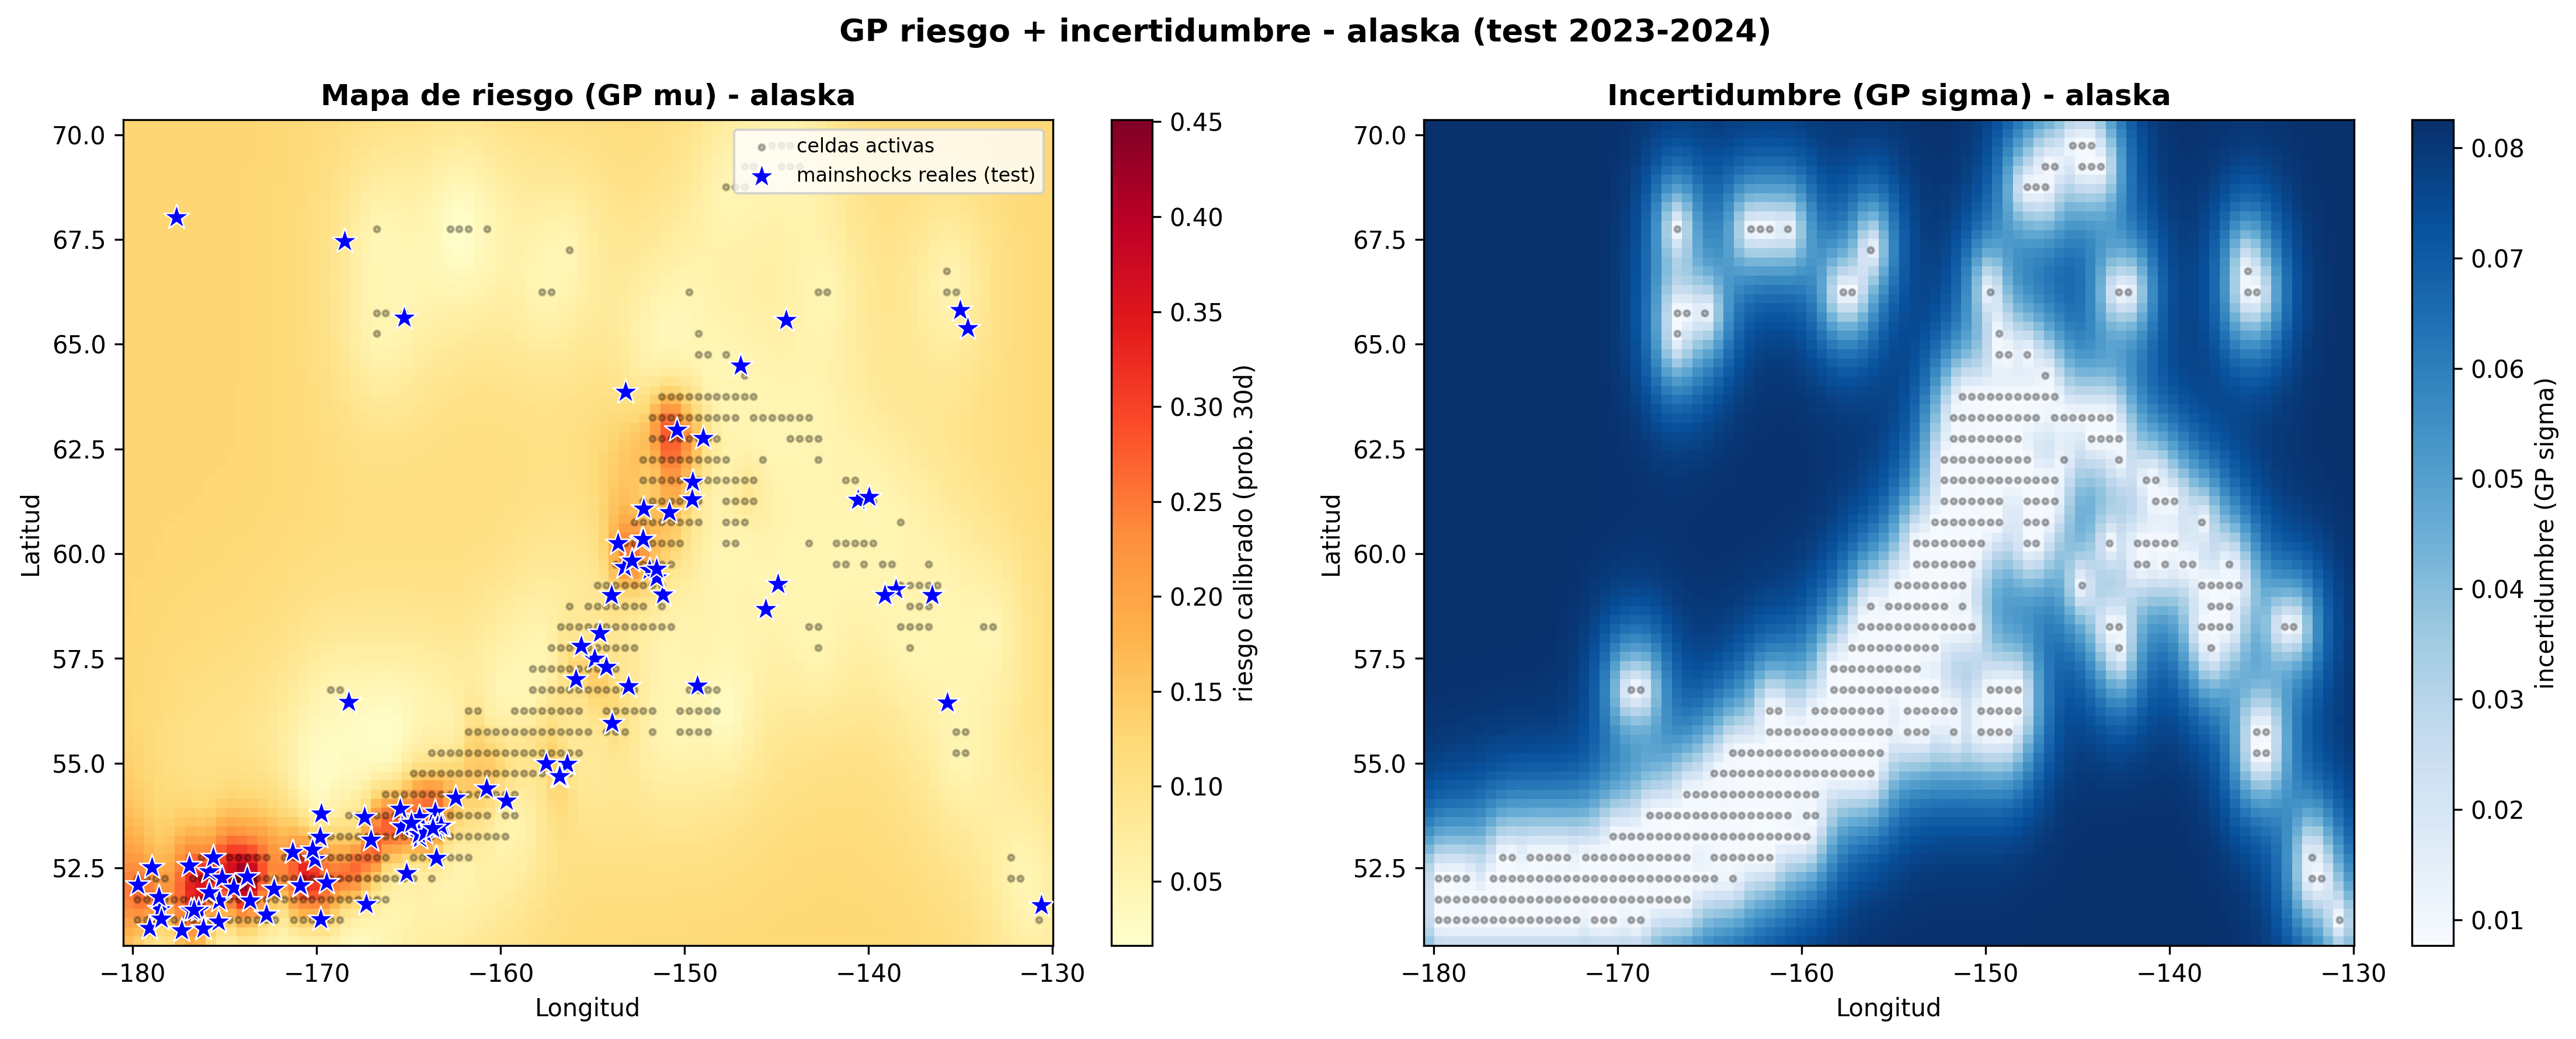
\includegraphics[width=\textwidth]{figuras/06_mapa_riesgo_gp_alaska}
  \caption[Mapa de riesgo e incertidumbre para Alaska]{\textbf{Mapa de riesgo (izquierda) e incertidumbre (derecha) para Alaska.} El riesgo se concentra en el arco de las Aleutianas y la costa sur. La incertidumbre crece en las zonas interiores sin sismicidad registrada.}
  \label{fig:mapaalaska}
\end{figure}

Para validar de forma cuantitativa la coherencia espacial del mapa se comprueba si los mainshocks
reales del test caen en las zonas de riesgo alto. El mapa distingue las celdas que registraron
mainshocks de las que no con un AUC de \textbf{0.80}, y asigna a las primeras un riesgo medio
\textbf{2.2 veces superior} al de las segundas. Esto confirma con números lo que se aprecia a
simple vista: el mapa concentra correctamente el riesgo en las zonas donde efectivamente ocurren
los terremotos.

\subsection{Generalización a otras regiones del mundo}
\label{res-transferencia}

Una pregunta natural, y muy valorada en la literatura, es si el modelo aprende algo
\emph{universal} o algo \emph{específico} de las zonas con las que se entrenó. Como el
Transformer aprende una función de las características y de la geometría --no una memoria de
celdas concretas--, en principio puede aplicarse a una región distinta sin reentrenar. Para
comprobarlo se realizó un experimento de \textbf{transferencia}: se tomó el modelo entrenado en
California+Alaska y se aplicó, \emph{en inferencia y sin reentrenar}, a nueve regiones sísmicas
de los cinco continentes (dos por continente, salvo África, donde solo el Magreb reunió datos
suficientes), replicando exactamente el mismo cálculo de características y de objetivo. Para cada
región se comparó el modelo transferido con su propia climatología de Poisson local.

\begin{table}[ht!]
  \centering
  \small
  \begin{tabular}{@{}llccccc@{}}
    \toprule
    \textbf{Región}   & \textbf{Continente} & \textbf{$M_c$} & \textbf{Celdas} & \textbf{AUC modelo} & \textbf{AUC Poisson} & \textbf{AUC temporal} \\
    \midrule
    Cascadia (PNW)    & N.\ América         & 2.8            & 31              & 0.420               & 0.809                & 0.540                 \\
    México (Guerrero) & N.\ América         & 4.0            & 64              & 0.538               & 0.600                & 0.517                 \\
    Chile norte       & S.\ América         & 4.2            & 155             & 0.511               & 0.708                & 0.511                 \\
    Perú              & S.\ América         & 4.2            & 45              & 0.479               & 0.605                & 0.541                 \\
    Italia (Apeninos) & Europa              & 2.8            & 33              & 0.441               & 0.647                & 0.556                 \\
    Grecia (Egeo)     & Europa              & 3.2            & 172             & 0.494               & 0.688                & 0.475                 \\
    Japón             & Asia                & 4.4            & 188             & \textbf{0.637}      & 0.723                & 0.465                 \\
    Sumatra           & Asia                & 4.4            & 94              & 0.545               & 0.656                & 0.552                 \\
    Magreb            & África              & 2.8            & 17              & 0.472               & 0.687                & 0.613                 \\
    \midrule
    \textbf{Media}    &                     &                &                 & \textbf{0.504}      & 0.671                & 0.530                 \\
    \bottomrule
  \end{tabular}
  \caption[Transferencia del Transformer a otras regiones]{\textbf{Transferencia del Transformer (entrenado en California+Alaska) a otras regiones.} AUC-ROC del modelo aplicado en inferencia frente a la climatología de Poisson local de cada región. En las nueve regiones el modelo queda por debajo de su climatología local, y de media su AUC (0.504) es indistinguible del azar. La AUC temporal por celda permanece próxima a 0.5, como en las regiones de entrenamiento.}
  \label{tab:transferencia}
\end{table}

La Tabla~\ref{tab:transferencia} resume el resultado. En \textbf{las nueve regiones} el modelo
transferido obtiene un AUC inferior al de la climatología local, y su valor medio, 0.504, es
\emph{indistinguible del azar}. En cinco regiones el AUC cae incluso por debajo de 0.5, lo que
indica que el orden de riesgo aprendido en California+Alaska no solo deja de ser útil, sino que
llega a ser contraproducente fuera de su dominio. La AUC temporal por celda se mantiene en torno
a 0.5, igual que en casa. Es decir, el modelo \textbf{no generaliza}: el mapa espacial de peligro
que captura es específico de las zonas con las que se entrenó.

Este resultado, lejos de ser un inconveniente, delimita con precisión el alcance del sistema y
admite una lectura \textbf{tectónica} coherente. Las regiones donde el modelo transfiere
\emph{menos mal} son Japón (0.637) y Sumatra (0.545), que elevan la media de Asia (0.591) por
encima de la del resto de continentes (entre 0.47 y 0.50). Ambas son
\textbf{zonas de subducción muy activas} --el mismo régimen tectónico que Alaska, una de las dos
regiones de entrenamiento-- en las que la sismicidad se alinea de forma marcada a lo largo de la
fosa. Esa estructura espacial intensa y bien definida es la que el mecanismo de atención puede
aprovechar parcialmente, aun aplicado fuera de su dominio. En el extremo opuesto, las regiones
donde peor transfiere son Cascadia (0.420), una zona de subducción \emph{bloqueada} y
sísmicamente tranquila en su interfaz, e Italia (0.441), de tectónica extensional difusa: en
ambas la geometría de la sismicidad se parece poco a la de California o Alaska. Las zonas de
subducción de Sudamérica (Chile, Perú) y de México quedan en una posición intermedia, penalizadas
además por una magnitud de completitud alta (en torno a $M_c \approx 4$) que empobrece sus
características. Conviene subrayar que ni siquiera Japón, la región más favorable, supera a su
climatología local: la similitud tectónica con Alaska ayuda, pero no basta para reconstruir el
mapa de peligro específico de otra región. En conjunto, el experimento confirma de forma directa
el hallazgo central del trabajo: el valor del sistema está en cartografiar la estructura
\emph{espacial} del peligro allí donde se entrena, y esa estructura es propia de cada región.

\subsection{Discusión de los resultados en el contexto del estado del arte}
\label{res-discusion}

Conviene situar los resultados anteriores en el marco de lo que la comunidad sismológica
considera alcanzable. El pronóstico de terremotos a corto plazo es, posiblemente, uno de los
problemas abiertos más difíciles de la geofísica, y la postura mayoritaria es que no existe un
método capaz de anticipar de forma fiable el instante de un sismo concreto con semanas de
antelación \citep{geller1997unpredictable, jordan2011oef}. Los sistemas operacionales más consolidados, como los basados en modelos de tipo
ETAS, no predicen tanto el \emph{momento} de un evento aislado como la \emph{tasa esperada} de
sismicidad, que aumenta tras un terremoto grande por el efecto de las réplicas \citep{ogata1988etas, marzocchi2014oef}. En ese contexto,
los resultados de este trabajo encajan de forma natural y coherente.

El primer punto de contacto es el papel de la climatología. En la evaluación de pronósticos
sísmicos es habitual que el listón a batir sea un modelo de tasa de fondo, precisamente porque
una parte muy grande de la ``predictibilidad'' de los terremotos se reduce a saber qué zonas son
crónicamente activas \citep{helmstetter2006comparison}. Que el Transformer iguale y supere ligeramente a la climatología de
Poisson, de forma estadísticamente significativa, es un resultado sólido: muchos métodos
sofisticados de la literatura no consiguen batir esta referencia de manera consistente
\citep{zechar2008testing, beroza2021dlreview}. Un caso ilustrativo es el de
\citet{devries2018aftershocks}, cuya red profunda para la predicción espacial de réplicas fue
posteriormente igualada por un \textit{baseline} de una sola neurona \citep{mignan2019oneneuron}. El
sistema, por tanto, se sitúa en el lado correcto de esa frontera.

El segundo punto, y el más importante, es la localización de la señal. El análisis con la AUC
temporal por celda muestra que la capacidad del sistema reside en la dimensión espacial y no en
la temporal a 30 días. Esta conclusión está en plena sintonía con el consenso científico: la
acumulación de tensión tectónica que conduce a un terremoto se desarrolla a lo largo de años y
de forma silenciosa \citep{stein2003introduction}, por lo que es razonable que un catálogo de eventos discretos no contenga la
firma precursora del momento exacto. Lo relevante de este trabajo no es, por tanto, ``descubrir''
que el pronóstico temporal es difícil --algo bien sabido-- sino \emph{medirlo con una métrica
  limpia} que separa ambas dimensiones, evitando la confusión, frecuente en la literatura aplicada,
entre acertar dónde y acertar cuándo. Un AUC global de 0.73 podría presentarse, sin este
análisis, como una capacidad de pronóstico temporal que en realidad no existe.

El tercer punto es la comparación entre arquitecturas. El hecho de que la GNN y el Transformer
--dos formas muy distintas de modelar el espacio-- lleguen esencialmente a la misma conclusión
refuerza su validez: no se trata de un artefacto de un diseño concreto, sino de una propiedad del
problema y de los datos. Esta convergencia entre métodos independientes es justamente el tipo de
evidencia que da credibilidad a un hallazgo.

El cuarto punto lo aporta el experimento de transferencia (Sección~\ref{res-transferencia}). Que
el modelo no generalice a otras regiones encaja con lo que cabe esperar de un sistema que, según
el análisis anterior, aprende fundamentalmente un \emph{mapa espacial de peligro}: dado que la
geometría de la sismicidad es propia de cada contexto tectónico, un mapa ajustado a la falla de
San Andrés y al arco de las Aleutianas no tiene por qué servir para la subducción andina o la
extensión del Egeo. La lectura tectónica de los resultados --el modelo transfiere algo mejor a las
subducciones muy activas de Asia, parecidas a Alaska, y peor a las zonas de geometría difusa o
tranquila-- es coherente con esta interpretación y, a la vez, marca el camino para mejorar: la
generalización exigiría reentrenar con datos de cada región o emplear técnicas de adaptación de
dominio, un problema bien documentado al transferir modelos profundos en sismología entre
conjuntos de datos y regiones distintas \citep{munchmeyer2022picker}. En conjunto, los resultados no solo son compatibles con el estado del arte, sino que
aportan una forma más honesta y precisa de evaluar este tipo de sistemas --separando el dónde del
cuándo y midiendo explícitamente la transferibilidad-- que es una contribución metodológica de
valor más allá del caso concreto estudiado.

\subsection{Síntesis de los resultados}
\label{res-sintesis}

En conjunto, los resultados dibujan un sistema que cumple su objetivo de extremo a extremo. La
detección funciona con alta fidelidad; los modelos espaciales capturan con éxito la estructura del
peligro sísmico y el mejor de ellos, el Transformer, supera de forma significativa a la
climatología; las métricas operativas confirman una capacidad de alerta cuatro veces superior al
azar; y el proceso gaussiano produce mapas de riesgo calibrados y acompañados de incertidumbre. El
análisis de la dimensión temporal, mediante una métrica diseñada al efecto, localiza con precisión
la información predictiva en la componente espacial y muestra que el horizonte temporal de 30 días
sobre el catálogo no aporta señal adicional, un resultado riguroso y alineado con el estado del
arte. El experimento de transferencia a nueve regiones de los cinco continentes completa el
diagnóstico: el sistema no generaliza fuera de su dominio de entrenamiento, lo que confirma que su
capacidad consiste en cartografiar la estructura espacial del peligro, propia de cada región, y no
en un patrón universal. El siguiente capítulo interpreta estos hallazgos a la luz de los objetivos
planteados.

\cleardoublepage

\chapter{Conclusiones y trabajos futuros}
\label{conclusion-y-trabajos-futuros}

Este capítulo cierra la memoria. Primero recoge las conclusiones del trabajo en relación con
los objetivos planteados al inicio, valorando en qué medida se han alcanzado y qué aporta cada
fase del sistema. A continuación reflexiona sobre las dificultades encontradas durante el
desarrollo, tanto las de naturaleza física como las de carácter práctico. Por último, propone
un conjunto de líneas de continuación ordenadas por ambición, que prolongan de forma natural lo
realizado.

\section{Conclusiones}
\label{conclusiones}

El objetivo general de este Trabajo de Fin de Máster era diseñar, implementar y validar un
\textit{pipeline} de aprendizaje profundo de extremo a extremo capaz de detectar eventos
sísmicos, modelar patrones de actividad y generar mapas de riesgo a corto plazo, con un nivel
de rigor metodológico comparable al de las publicaciones del área. A la luz de los resultados
del capítulo anterior, puede afirmarse que ese objetivo se ha cumplido: el sistema integra
cinco modelos en un flujo coherente y reproducible, y cada fase aporta un resultado claro y
verificable. Más allá de construir el sistema, el trabajo ha conseguido algo igualmente
valioso, que es \emph{medir con honestidad} qué parte del problema es abordable con los datos
disponibles y qué parte no, distinción que constituye la principal aportación científica de la
memoria. A continuación se detallan las conclusiones por objetivos parciales.

\paragraph{Construcción de una base experimental reproducible.} Se ha construido un conjunto
de datos coherente a partir de dos fuentes abiertas, STEAD para las formas de onda y el
catálogo del USGS para el pronóstico, con regiones, ventanas y umbrales justificados. Un
análisis empírico ha mostrado por qué cada fuente es adecuada para su tarea: STEAD aporta
trazas etiquetadas de alta calidad para detección, mientras que el catálogo USGS ofrece la
cobertura completa y homogénea que exige el cálculo de características de pronóstico, como
confirmó la comparación directa entre ambos catálogos. Todas las decisiones de preprocesado
--magnitud de completitud, aislamiento de eventos independientes mediante
\textit{declustering}, particiones estrictamente temporales y normalización ajustada solo en
entrenamiento-- se han tomado con criterios documentados y reproducibles. Este cuidado
metodológico, lejos de ser un detalle accesorio, es lo que permite confiar en las conclusiones
posteriores: sin él, cualquier resultado quedaría en entredicho por posibles fugas de
información.

\paragraph{Detección y \textit{picking} de fases.} Las arquitecturas preentrenadas PhaseNet y
EQTransformer alcanzan un rendimiento alto sobre datos no vistos, con un \textit{F1-score} de
hasta 0.93 en la fase P --que asciende por encima de 0.96 si se relaja ligeramente la
tolerancia temporal-- y errores de localización de pocas centésimas de segundo, comparables a
los de un analista humano. Esto confirma que la detección automática de fases es hoy una tarea
resuelta de forma fiable mediante aprendizaje profundo, y proporciona una base firme sobre la
que apoyar el resto del sistema. La elección de dos arquitecturas de familias distintas --una
\textit{U-Net} convolucional y una red multitarea con atención-- ha permitido además comprobar
que el resultado no depende de un diseño concreto.

\paragraph{Modelado de la dimensión temporal y espacial.} El trabajo ha contrastado de forma
sistemática un enfoque puramente temporal frente a uno espacial. El modelo temporal global no
supera a las referencias, lo que indica que la evolución temporal agregada de la sismicidad no
contiene, por sí sola, información suficiente para el pronóstico. La incorporación de la
dimensión espacial, en cambio, sí produce una mejora sustancial: tanto la red de grafos como el
Transformer geoespacial alcanzan un AUC en torno a 0.70--0.73, y el Transformer supera a la
climatología de Poisson de forma estadísticamente significativa. La representación del espacio
se revela, por tanto, como el factor decisivo, y el mecanismo de atención del Transformer
resulta ligeramente más eficaz que la propagación por grafo de la GNN. Este resultado tiene
valor práctico inmediato: orienta el diseño de futuros sistemas hacia las arquitecturas que
modelan explícitamente la estructura espacial de la sismicidad.

\paragraph{Localización de la información predictiva.} La aportación metodológica más relevante
del trabajo es la separación explícita de las dos preguntas que encierra el problema --dónde y
cuándo-- mediante una métrica diseñada al efecto, la AUC temporal por celda. Su aplicación
permite afirmar con precisión que la capacidad del sistema reside en la dimensión espacial: el
modelo identifica muy bien las zonas crónicamente peligrosas, mientras que la anticipación
temporal a 30 días, una vez aislada del componente espacial, coincide con la tasa base. Este
resultado, confirmado por varios estudios de ablación que lo mantienen estable frente a cambios
de arquitectura, de ventana y de preprocesado, es plenamente coherente con el consenso
científico actual sobre la dificultad del pronóstico a corto plazo. Constituye un hallazgo
honesto y bien fundamentado, más valioso que una cifra global que mezclase ambas dimensiones y
diese una impresión inflada del rendimiento. Saber con certeza dónde reside --y dónde no-- la
información aprovechable es, en sí mismo, un avance.

\paragraph{Alcance y generalización del modelo.} Un experimento de transferencia a nueve regiones
de los cinco continentes ha permitido delimitar con precisión el alcance del sistema. Aplicado sin
reentrenar fuera de California+Alaska, el modelo no generaliza: en todas las regiones queda por
debajo de su climatología local y su AUC medio (0.504) es indistinguible del azar. Este resultado,
lejos de restar valor al trabajo, lo precisa: confirma que lo que el sistema aprende es el
\emph{mapa espacial de peligro} de las zonas con las que se entrenó, una estructura propia de cada
contexto tectónico y no un patrón universal. La lectura del experimento es además coherente con la
física: el modelo transfiere algo mejor a las subducciones muy activas de Asia --semejantes a la
de Alaska-- y peor a las regiones de geometría difusa o sísmicamente tranquila. Queda así claro
que el sistema es una herramienta de cartografía \emph{regional}, que debe ajustarse a cada zona,
y no un pronosticador global.

\paragraph{Cuantificación de la incertidumbre y mapas de riesgo.} La capa final basada en un
proceso gaussiano cierra el \textit{pipeline} produciendo mapas continuos de riesgo acompañados
de su incertidumbre. La calibración previa de las probabilidades, validada de forma
independiente sobre una partición reservada, reduce el \textit{Brier score} en dos tercios, de
modo que los mapas expresan frecuencias de ocurrencia realistas y no valores inflados por la
ponderación de clase. La validación cuantitativa confirma que los mapas concentran el riesgo en
las zonas donde efectivamente ocurren los terremotos, con un AUC espacial de 0.80 y un riesgo
medio más del doble en las celdas con eventos reales. El mapa de incertidumbre, además, crece de
forma coherente en las zonas con menos datos, lo que comunica al usuario dónde debe confiar más
y dónde menos en la predicción. El sistema entrega, así, un producto cartográfico accionable y
honesto sobre su propia confianza.

\medskip
En conjunto, el trabajo demuestra que un \textit{pipeline} de aprendizaje profundo construido
con rigor es capaz de cartografiar el peligro sísmico espacial con calidad y de acotar con
precisión los límites de la predicción temporal a corto plazo. Esta combinación --un producto
útil y una delimitación honesta de lo que es y no es posible-- es, precisamente, lo que
distingue a un trabajo metodológicamente sólido de una mera optimización de cifras. El sistema
no solo responde a la pregunta que se le plantea, sino que sabe explicar con datos por qué
responde mejor a unas preguntas que a otras, lo que lo convierte en una herramienta fiable
sobre la que seguir construyendo.

\section{Limitaciones y dificultades}
\label{limitaciones}

El desarrollo del trabajo ha encontrado varias dificultades que conviene explicitar, tanto por
honestidad científica como porque orientan con claridad las líneas futuras.

La principal limitación es de naturaleza física y no metodológica: la información necesaria para
anticipar el \emph{momento} de un terremoto a 30 días no parece estar presente en el catálogo de
eventos. La acumulación de tensión que precede a un sismo se produce en escalas de tiempo de
años y de forma mayoritariamente silenciosa, por lo que apenas queda registrada en una secuencia
de eventos discretos. Esto sitúa un techo a lo que cualquier modelo puede aprender de esta fuente
de datos, con independencia de su sofisticación; es importante subrayar que se trata de un límite
de la \emph{información disponible}, no del método empleado, y que ese límite ha sido medido, no
supuesto. Reconocerlo con precisión es preferible a presentar un resultado optimista que no
resistiría una evaluación rigurosa.

Una segunda limitación es el fuerte desbalance del problema y la rareza de los eventos objetivo,
que reduce la potencia estadística y obliga a un tratamiento muy cuidadoso de las métricas.
Aunque la unión de California y Alaska mitiga el problema al aumentar el número de casos
positivos, el número de mainshocks independientes sigue siendo modesto en términos de aprendizaje
automático, lo que aconseja interpretar las diferencias pequeñas con cautela y apoyarlas siempre
en tests estadísticos, como se ha hecho a lo largo del trabajo.

Una tercera limitación es de alcance: el modelo trabaja con una resolución espacial de media
décima de grado y un horizonte fijo de 30 días. Resoluciones más finas o horizontes distintos
podrían cambiar el equilibrio entre las dimensiones espacial y temporal, y no se han explorado de
forma exhaustiva por el coste computacional que implica reentrenar todo el \textit{pipeline} para
cada configuración.

Por último, una dificultad de carácter práctico ha sido la gestión de la reproducibilidad en un
entorno de cómputo en la nube, el control de las numerosas configuraciones experimentales y la
coherencia entre los resultados de las distintas fases. Estas dificultades se han abordado con un
registro detallado de cada iteración, con la fijación de todas las semillas aleatorias y con un
protocolo de evaluación uniforme entre modelos, lo que ha permitido que las comparaciones sean
siempre justas y repetibles.

\section{Trabajos futuros}
\label{trabajos-futuros}

Los resultados sugieren varias líneas de continuación, ordenadas de menor a mayor ambición. Todas
ellas parten de una base sólida --el sistema actual funciona y su evaluación es fiable-- y buscan
ampliar, bien el alcance del producto, bien la frontera de lo que es posible aprender.

\paragraph{Horizontes temporales más cortos.} Dado que la señal precursora, de existir, vive en
escalas de días más que de semanas, una línea natural es reducir la ventana de predicción a 7 o
14 días y estudiar si en ese régimen aparece alguna capacidad temporal, manteniendo la
formulación espacial que ha demostrado funcionar. Esta exploración es de bajo coste, porque
reutiliza por completo la infraestructura existente, y permitiría trazar una curva de
rendimiento frente al horizonte que delimitaría con más finura la frontera temporal del
pronóstico.

\paragraph{Información de forma de onda.} El presente trabajo modela el pronóstico a partir del
catálogo de eventos, que es una representación discreta y muy comprimida de la actividad
sísmica. Una extensión prometedora, aunque costosa, consiste en incorporar características
derivadas de las propias formas de onda --contenido espectral, cambios en la velocidad sísmica
del medio, tremor de baja frecuencia-- que podrían contener información precursora ausente en el
catálogo. Esto requeriría procesar señal continua de las estaciones, una fuente de datos mucho
más voluminosa, pero es quizá la vía con mayor potencial para superar el techo identificado en
este trabajo.

\paragraph{Adaptación de dominio entre regiones.} El experimento de transferencia
(Sección~\ref{res-transferencia}) ha mostrado que el modelo entrenado en California+Alaska no
generaliza sin más a otras regiones: los patrones espaciales que aprende son específicos de cada
contexto tectónico. La línea natural de continuación es, por tanto, abordar la
\textbf{adaptación de dominio}: reentrenar o reajustar el modelo con datos de la región objetivo,
o entrenar un único modelo sobre un conjunto amplio y diverso de regiones para que aprenda
representaciones más transferibles. Sería especialmente interesante comprobar si un modelo
entrenado conjuntamente sobre varias subducciones generaliza mejor a una subducción nueva que el
modelo actual, lo que confirmaría que la similitud tectónica es la variable clave. Este tipo de
estudio, muy valorado en la literatura, es el paso obligado de cara a un despliegue fuera de la
región de entrenamiento.

\paragraph{Arquitecturas y características adicionales.} En el plano del modelado, se podrían
explorar mecanismos de atención más expresivos, redes de grafos con aristas ponderadas por la
distancia o por la conectividad tectónica conocida, y características derivadas de catálogos de
fallas. Cualquiera de estas mejoras se integraría sin cambios en el protocolo de evaluación, lo
que facilitaría medir su aportación real frente a las referencias actuales.

\paragraph{Calibración predictiva y validación operacional.} La calibración empleada para los
mapas se ha validado sobre una partición independiente del periodo de test, lo que ya evita la
circularidad. Una línea de mejora consiste en ajustar la calibración de forma prospectiva,
actualizándola a medida que llegan nuevos datos, y en evaluar el sistema en el formato del
diagrama de Molchan frente a los sistemas operacionales de referencia, lo que situaría los
resultados en el marco de comparación estándar de la sismología y acercaría el prototipo a un
uso real.

\paragraph{Fusión de fuentes y producto cartográfico.} Finalmente, combinar el catálogo del USGS
con catálogos relocalizados de mayor precisión, o con información geológica de fallas y de
deformación medida por GPS, podría enriquecer las características espaciales y refinar los mapas
de riesgo. Sobre esa base se podría construir un producto cartográfico interactivo y actualizado
de forma periódica, manteniendo siempre el mismo \textit{pipeline} de evaluación que garantiza la
fiabilidad de los resultados.

\medskip
En definitiva, este trabajo aporta un sistema completo y una metodología de evaluación rigurosa
que no solo entrega un producto útil --la cartografía del peligro sísmico con incertidumbre-- sino
que también delimita con honestidad la frontera actual de la predicción temporal a corto plazo.
Esa delimitación, lejos de ser un punto final, marca el comienzo de las líneas de investigación
más prometedoras: sabiendo con precisión dónde está el límite, es posible dirigir el esfuerzo
futuro exactamente hacia donde puede dar fruto. Esa es, quizá, la contribución más duradera de
esta memoria.


\glsaddall
\printglossary[type=\acronymtype]
\printglossary

\appendix
\cleardoublepage

\chapter{Apéndice I}
\label{apendice-i}

Este apéndice reúne el material propio que complementa la memoria pero que, incluido en los
capítulos, habría interrumpido el hilo de la lectura: las tablas con los resultados completos, el
detalle de las pruebas estadísticas y la información necesaria para reproducir el trabajo.

\section{Hiperparámetros completos de los modelos de pronóstico}
\label{apendice-hiperparametros}

Esta sección recoge, con fines de reproducibilidad, el conjunto completo de hiperparámetros de
los tres modelos de pronóstico (TCN, GNN y Transformer geoespacial), tal y como se han fijado en
los \textit{notebooks} de entrenamiento. Para mayor claridad se han separado en dos bloques: los
hiperparámetros de \textbf{arquitectura}, que definen la estructura de cada red
(Tabla~\ref{tab:hiper-arq}), y los de \textbf{entrenamiento}, que controlan el proceso de
optimización (Tabla~\ref{tab:hiper-train}). En el cuerpo de la memoria, la
Tabla~\ref{tab:hiperparametros} resume únicamente los más relevantes.

\begin{table}[ht!]
  \centering
  \small
  \begin{tabular}{@{}lccc@{}}
    \toprule
    \textbf{Hiperparámetro de arquitectura} & \textbf{TCN}                                & \textbf{GNN}  & \textbf{Transformer}     \\
    \midrule
    Características de entrada              & 5                                           & 5             & 5                        \\
    Canales de la TCN                       & (32,32,64,64)                               & (32,32,64)    & (32,32,64)               \\
    Niveles / dilataciones                  & 4 / \{1,2,4,8\}                             & 3 / \{1,2,4\} & 3 / \{1,2,4\}            \\
    Tamaño de \textit{kernel}               & 3                                           & 3             & 3                        \\
    Campo receptivo (días)                  & 61                                          & 29            & 29                       \\
    \textit{Pooling} temporal               & \multicolumn{3}{c}{[último, media, máximo]}                                            \\
    Dim.\ de \textit{embedding} espacial    & ---                                         & 64 (GCN)      & 128 ($D_{\text{model}}$) \\
    Capas espaciales                        & ---                                         & 2 (GCN)       & 2 (codificador)          \\
    Cabezas de atención                     & ---                                         & ---           & 4                        \\
    Dim.\ \textit{feed-forward}             & ---                                         & ---           & 256                      \\
    \textit{Dropout}                        & 0.20                                        & 0.15          & 0.20                     \\
    \bottomrule
  \end{tabular}
  \caption[Hiperparámetros de arquitectura de los modelos de pronóstico]{\textbf{Hiperparámetros de arquitectura} de los tres modelos de pronóstico. El campo receptivo se obtiene de la relación~\eqref{eq:rf-tcn}; todos comparten la misma TCN como bloque temporal y el mismo \textit{pooling} de tres estadísticos.}
  \label{tab:hiper-arq}
\end{table}

\begin{table}[ht!]
  \centering
  \small
  \begin{tabular}{@{}lccc@{}}
    \toprule
    \textbf{Hiperparámetro de entrenamiento} & \textbf{TCN}                                                                  & \textbf{GNN}     & \textbf{Transformer} \\
    \midrule
    Optimizador                              & Adam                                                                          & Adam             & Adam                 \\
    Tasa de aprendizaje inicial              & $3\times10^{-4}$                                                              & $3\times10^{-3}$ & $1\times10^{-4}$     \\
    Tamaño de lote (\textit{batch})          & 64                                                                            & 48               & 32                   \\
    Épocas máximas                           & 80                                                                            & 200              & 200                  \\
    Paciencia (parada temprana)              & 12                                                                            & 6                & 12                   \\
    Decaimiento de pesos ($L_2$)             & $10^{-4}$                                                                     & $10^{-4}$        & $10^{-4}$            \\
    Recorte de gradiente                     & 1.0                                                                           & 1.0              & 1.0                  \\
    Planificador de tasa                     & \multicolumn{3}{c}{\textit{ReduceLROnPlateau} sobre la métrica de validación}                                           \\
    Función de pérdida                       & \multicolumn{3}{c}{entropía cruzada binaria con ponderación de clase}                                                   \\
    Ventana de historia (\textit{lookback})  & 60 d                                                                          & 60 d             & 60 d                 \\
    Ventana de predicción                    & 14 d                                                                          & 30 d             & 30 d                 \\
    Semillas                                 & \multicolumn{3}{c}{\{13, 42, 123, 256, 1024\}}                                                                          \\
    \bottomrule
  \end{tabular}
  \caption[Hiperparámetros de entrenamiento de los modelos de pronóstico]{\textbf{Hiperparámetros de entrenamiento} de los tres modelos de pronóstico. Los tres comparten optimizador, planificador, tipo de pérdida y protocolo multi-semilla; difieren en la tasa de aprendizaje, el tamaño de lote y la duración del entrenamiento.}
  \label{tab:hiper-train}
\end{table}

\section{Validación empírica de la fuente de datos: STEAD frente a USGS}
\label{apendice-stead-usgs}

Una pregunta natural es por qué el pronóstico utiliza el catálogo del USGS y no el dataset STEAD,
que contiene más de un millón de trazas. La razón es que ambos sirven para tareas distintas:
STEAD es una selección curada de formas de onda para entrenar detectores, mientras que el
pronóstico necesita un catálogo \emph{completo} y \emph{homogéneo} en el tiempo. Las
Figuras~\ref{fig:steadcobertura} y~\ref{fig:steadmc} lo demuestran de forma empírica sobre
California.

\begin{figure}[ht!]
  \centering
  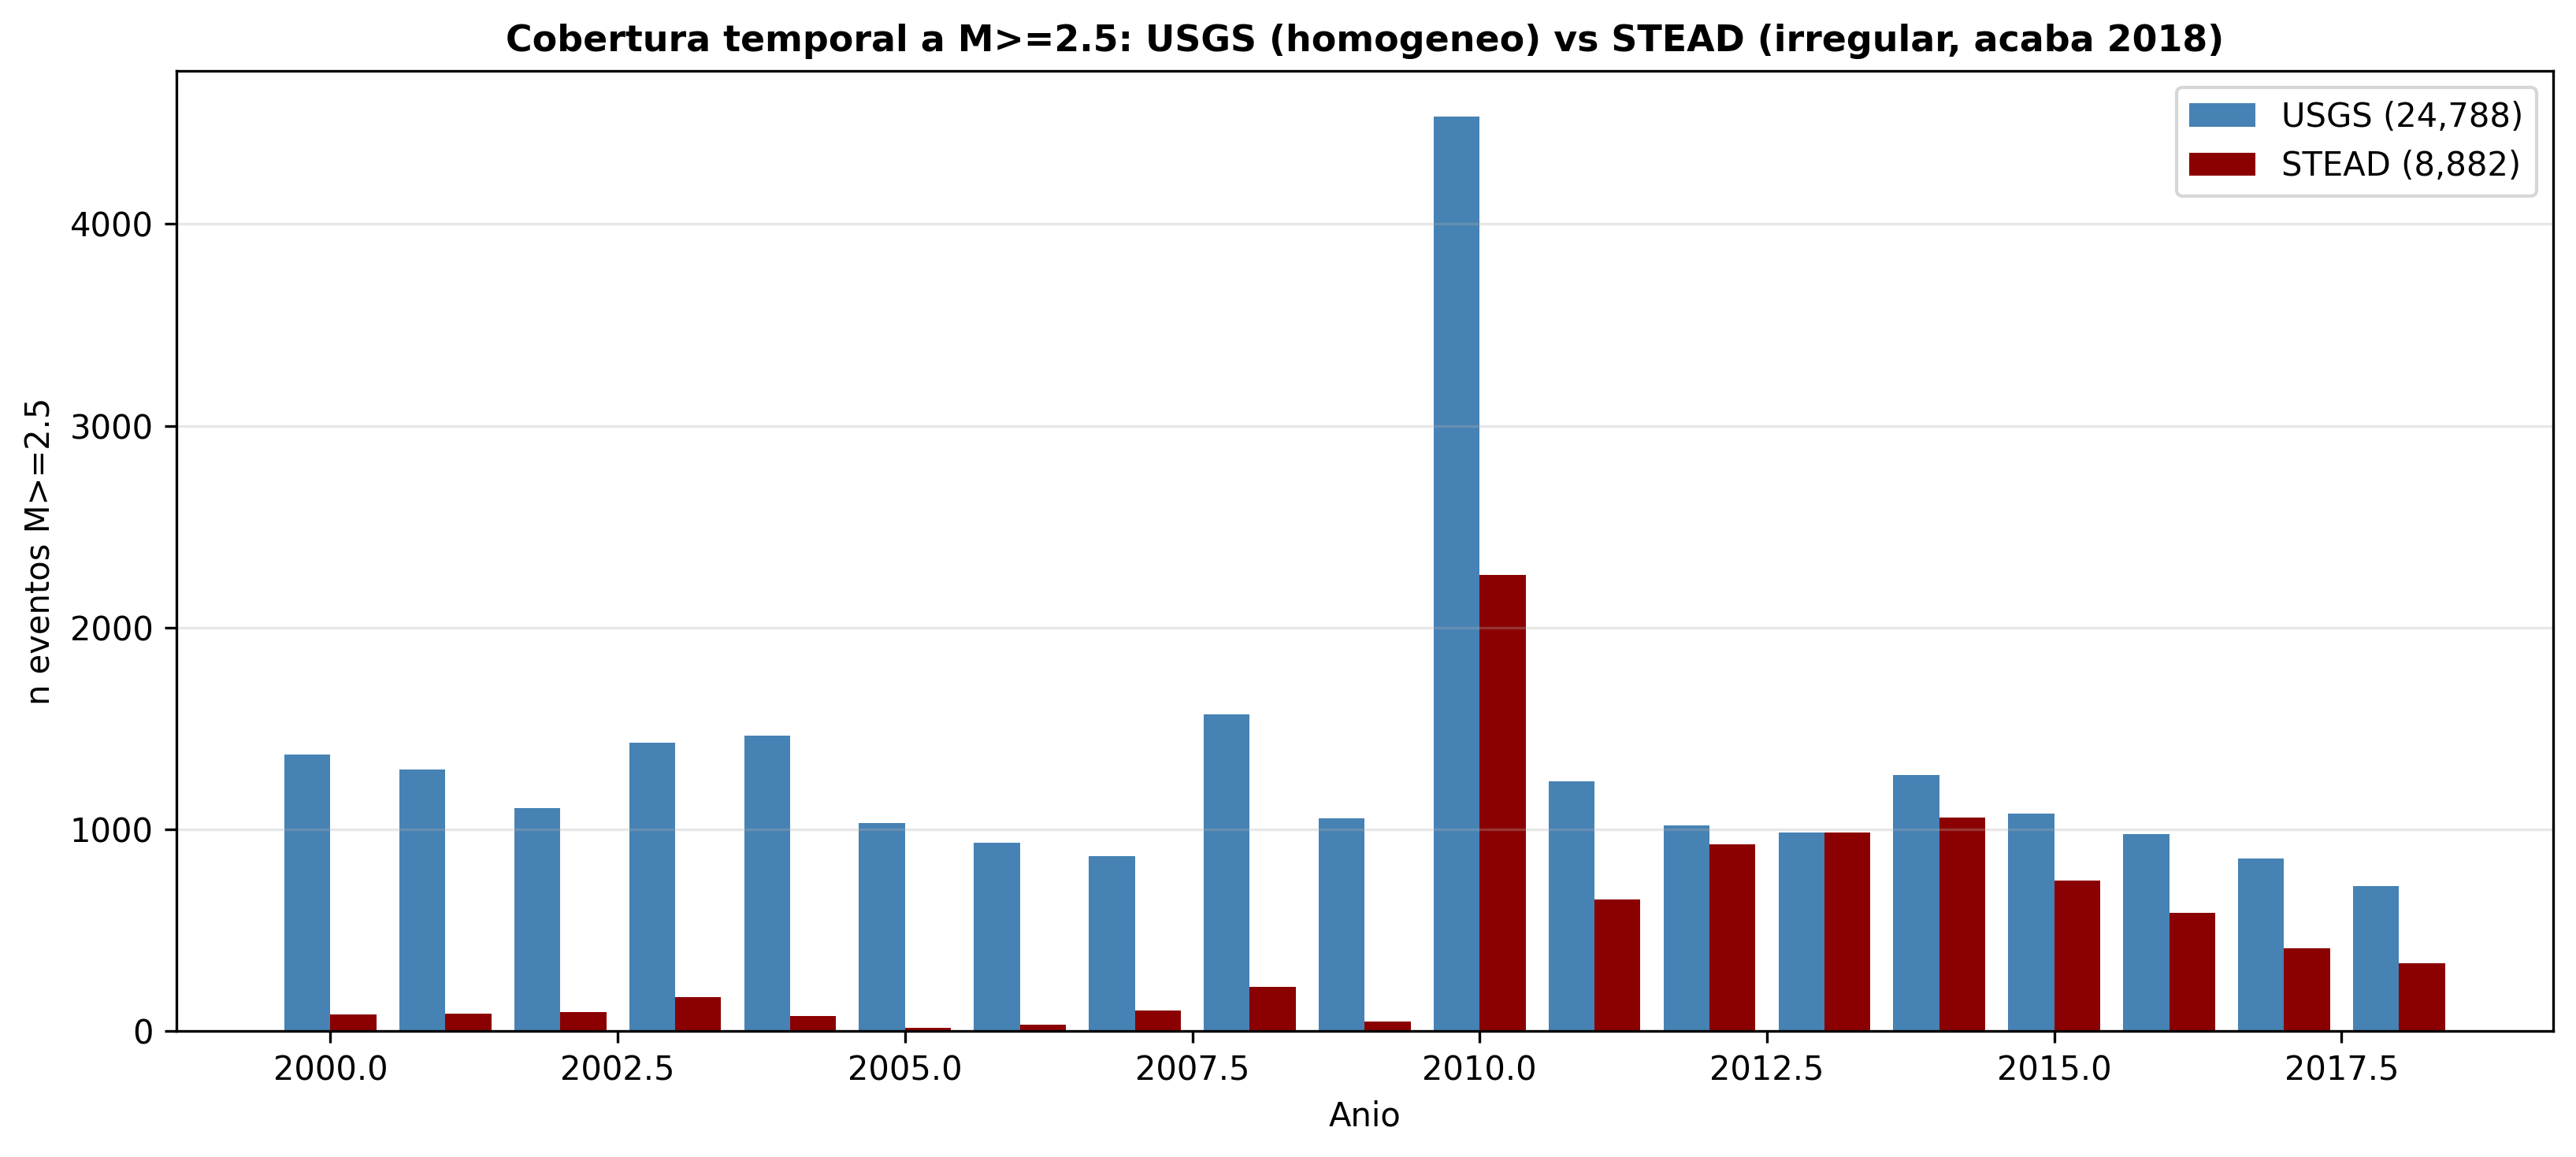
\includegraphics[width=0.92\textwidth]{figuras/07_stead_vs_usgs_cobertura}
  \caption[Cobertura temporal de STEAD frente a USGS]{\textbf{Número de eventos por año (\(M\geq 2.5\)) en California.} El catálogo USGS (azul) ofrece una cobertura continua y homogénea, mientras que STEAD (rojo) presenta un muestreo muy irregular y termina en 2018.}
  \label{fig:steadcobertura}
\end{figure}

\begin{figure}[ht!]
  \centering
  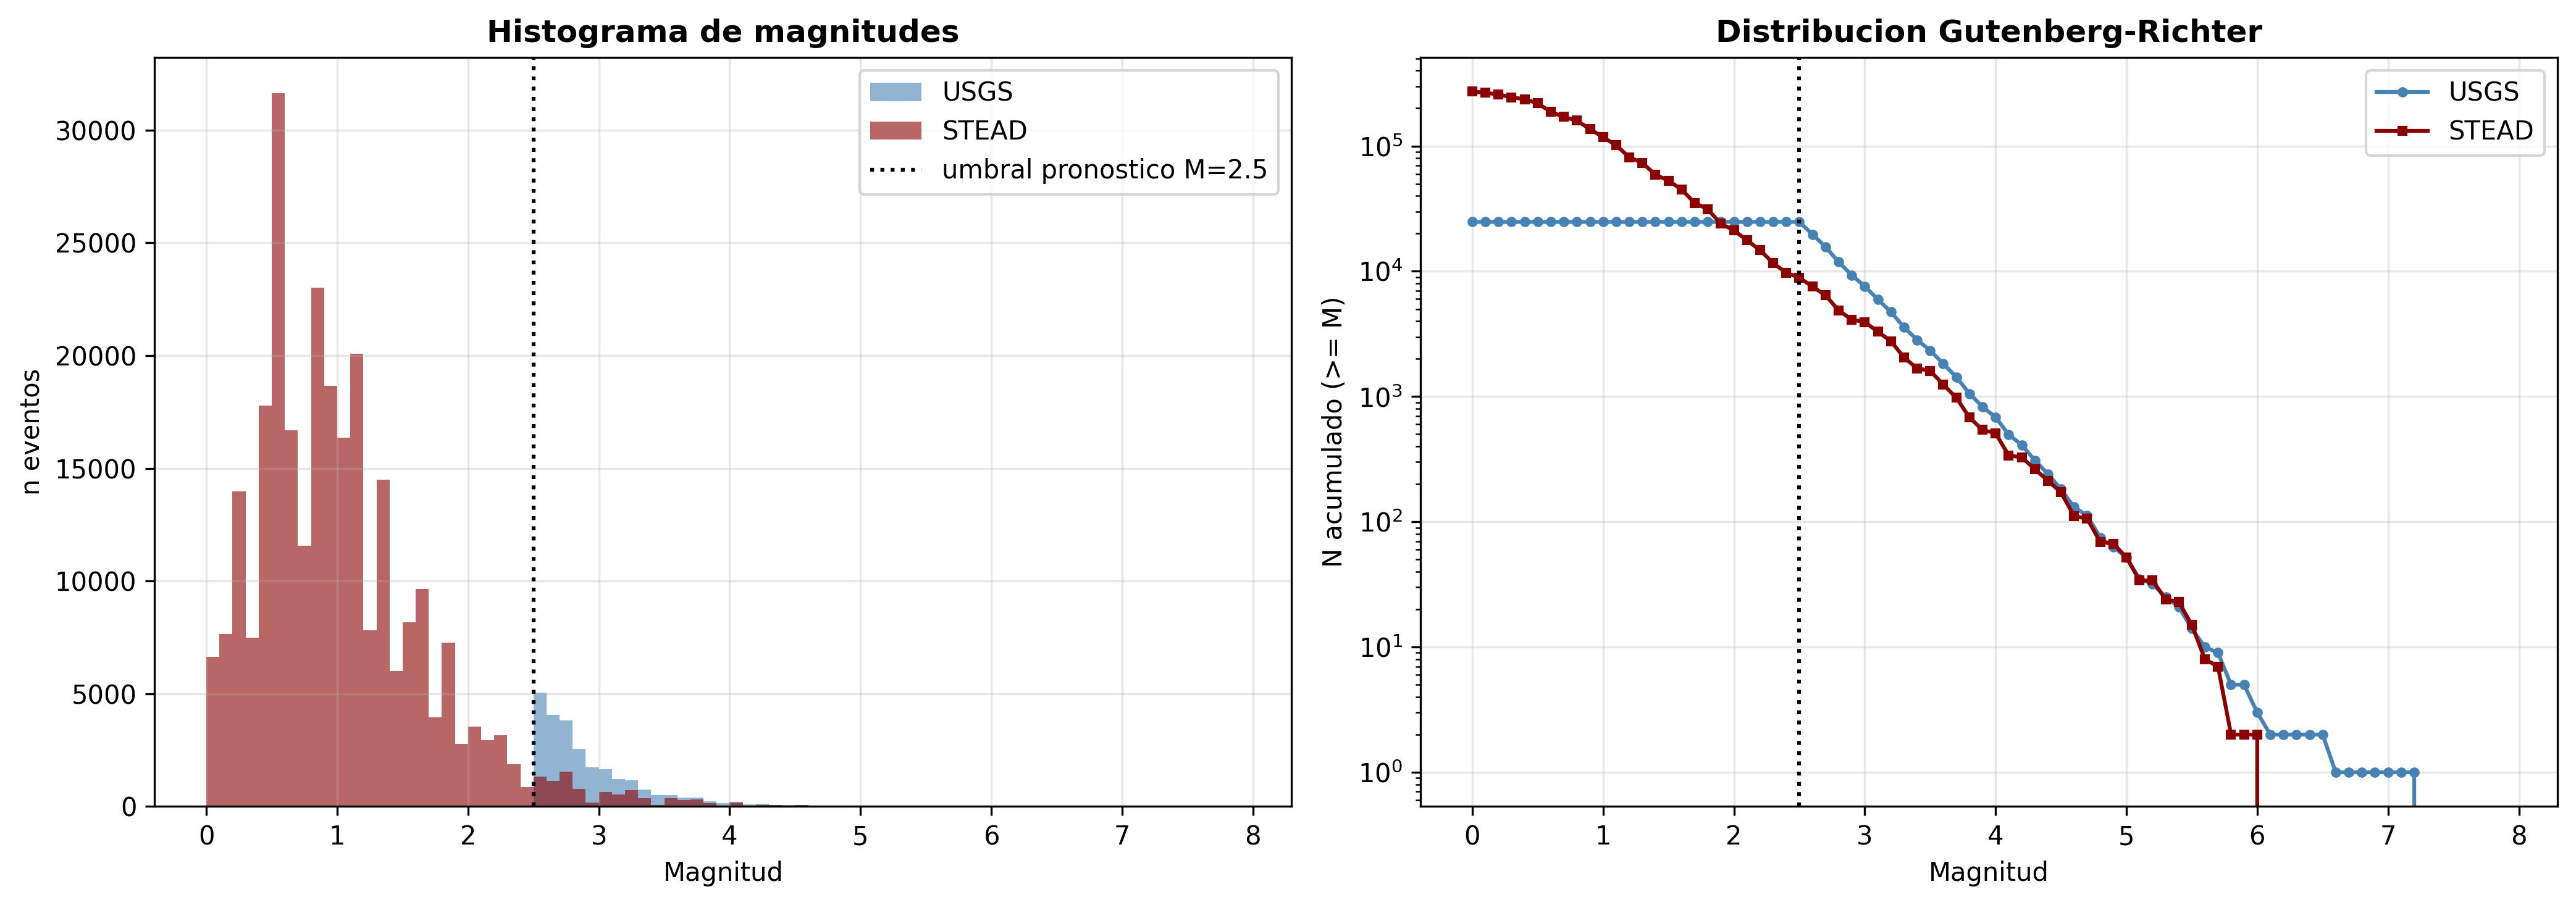
\includegraphics[width=0.92\textwidth]{figuras/07_stead_vs_usgs_magnitud_mc}
  \caption[Distribución de magnitudes y completitud de STEAD frente a USGS]{\textbf{Distribución de magnitudes (izquierda) y curva de Gutenberg--Richter (derecha)} para STEAD y USGS en California. La curva de USGS sigue una recta limpia por encima de la magnitud de completitud, mientras que la de STEAD presenta irregularidades propias de una selección curada.}
  \label{fig:steadmc}
\end{figure}

A igualdad de magnitud (\(M \geq 2.5\)), el USGS contiene en torno a tres veces más eventos que
STEAD en la misma región y periodo, lo que indica que STEAD es incompleto. Su muestreo por año
varía de forma artificial en hasta dos órdenes de magnitud, lo que distorsionaría cualquier
estadística de tasa, y además termina en 2018, por lo que no cubre el periodo de test. Por todo
ello, las características de pronóstico requieren el catálogo USGS, mientras que STEAD se reserva,
con todo su valor, para la fase de detección.

\section{Resultados completos de detección y \textit{picking}}
\label{apendice-deteccion}

La Tabla~\ref{tab:deteccion-completa} amplía la tabla del cuerpo con el rendimiento de PhaseNet y
EQTransformer en las dos fases (P y S) a varias tolerancias temporales, junto con los errores de
localización. Como es esperable, al ampliar la tolerancia mejoran \textit{precision}, \textit{recall}
y \textit{F1}, a costa de un error de localización ligeramente mayor.

\begin{table}[ht!]
  \centering
  \small
  \begin{tabular}{@{}llcccccc@{}}
    \toprule
    \textbf{Modelo} & \textbf{Fase} & \textbf{Tol.\ (s)} & \textbf{Precision} & \textbf{Recall} & \textbf{F1} & \textbf{MAE (s)} & \textbf{RMSE (s)} \\
    \midrule
    PhaseNet        & P             & 0.05               & 0.847              & 0.854           & 0.851       & 0.018            & 0.021             \\
    PhaseNet        & P             & 0.10               & 0.927              & 0.934           & 0.930       & 0.022            & 0.030             \\
    PhaseNet        & P             & 0.20               & 0.957              & 0.965           & 0.961       & 0.026            & 0.039             \\
    PhaseNet        & P             & 0.50               & 0.983              & 0.991           & 0.987       & 0.034            & 0.067             \\
    PhaseNet        & S             & 0.10               & 0.782              & 0.794           & 0.788       & 0.029            & 0.038             \\
    PhaseNet        & S             & 0.20               & 0.879              & 0.892           & 0.885       & 0.042            & 0.060             \\
    PhaseNet        & S             & 0.50               & 0.952              & 0.966           & 0.959       & 0.063            & 0.107             \\
    PhaseNet        & S             & 1.00               & 0.976              & 0.991           & 0.984       & 0.078            & 0.153             \\
    \midrule
    EQTransformer   & P             & 0.05               & 0.736              & 0.656           & 0.694       & 0.018            & 0.024             \\
    EQTransformer   & P             & 0.10               & 0.883              & 0.787           & 0.832       & 0.027            & 0.036             \\
    EQTransformer   & P             & 0.20               & 0.932              & 0.830           & 0.878       & 0.033            & 0.048             \\
    EQTransformer   & P             & 0.50               & 0.957              & 0.853           & 0.902       & 0.040            & 0.072             \\
    EQTransformer   & S             & 0.10               & 0.739              & 0.760           & 0.750       & 0.035            & 0.044             \\
    EQTransformer   & S             & 0.20               & 0.865              & 0.889           & 0.877       & 0.051            & 0.068             \\
    EQTransformer   & S             & 0.50               & 0.943              & 0.969           & 0.956       & 0.073            & 0.115             \\
    EQTransformer   & S             & 1.00               & 0.964              & 0.991           & 0.977       & 0.087            & 0.154             \\
    \bottomrule
  \end{tabular}
  \caption[Resultados completos de detección y \textit{picking}]{\textbf{Detección y \textit{picking} completos} de PhaseNet y EQTransformer sobre STEAD, por fase y tolerancia. MAE y RMSE son los errores de localización de la llegada, en segundos.}
  \label{tab:deteccion-completa}
\end{table}

\section{Métricas operativas completas}
\label{apendice-operativas}

La Tabla~\ref{tab:operativas-completa} detalla las métricas de alerta del Transformer y del Poisson
en los tres niveles de alarma (top 0.5\,\%, 1\,\% y 5\,\%), ampliando las que figuran en el cuerpo.

\begin{table}[ht!]
  \centering
  \small
  \begin{tabular}{@{}lcccccccc@{}}
    \toprule
                       & \multicolumn{2}{c}{\textbf{Top 0.5\,\%}} & \multicolumn{2}{c}{\textbf{Top 1\,\%}} & \multicolumn{2}{c}{\textbf{Top 5\,\%}} & \textbf{PR-AUC} &                                                       \\
    \cmidrule(lr){2-3}\cmidrule(lr){4-5}\cmidrule(lr){6-7}
    \textbf{Métrica}   & \textbf{Trans.}                          & \textbf{Pois.}                         & \textbf{Trans.}                        & \textbf{Pois.}  & \textbf{Trans.} & \textbf{Pois.} & \textbf{Tr./Po.} & \\
    \midrule
    \textit{Precision} & 0.183                                    & 0.160                                  & 0.187                                  & 0.186           & 0.150           & 0.151          & ---              & \\
    \textit{Recall}    & 0.020                                    & 0.018                                  & 0.042                                  & 0.041           & 0.167           & 0.168          & ---              & \\
    \textit{Lift}      & 4.07                                     & 3.56                                   & 4.17                                   & 4.14            & 3.35            & 3.36           & 0.111 / 0.110    & \\
    \bottomrule
  \end{tabular}
  \caption[Métricas operativas completas del Transformer y el Poisson]{\textbf{Métricas operativas completas.} \textit{Precision}, \textit{recall} y \textit{lift} del Transformer (Trans.) y del Poisson (Pois.) en el top 0.5\,\%, 1\,\% y 5\,\% de mayor riesgo, más la PR-AUC.}
  \label{tab:operativas-completa}
\end{table}

\section{Resultados completos de transferencia entre regiones}
\label{apendice-transferencia}

La Tabla~\ref{tab:transferencia-completa} recoge todas las métricas del experimento de
transferencia (Sección~\ref{res-transferencia}) para las nueve regiones evaluadas, incluyendo el
número de celdas activas, los eventos objetivo, la PR-AUC y el \textit{lift}.

\begin{table}[ht!]
  \centering
  \small
  \resizebox{\textwidth}{!}{%
    \begin{tabular}{@{}llcccccccc@{}}
      \toprule
      \textbf{Región}   & \textbf{Continente} & \textbf{$M_c$} & \textbf{Celdas} & \textbf{Objetivos} & \textbf{AUC mod.} & \textbf{AUC Pois.} & \textbf{PR-AUC} & \textbf{Lift@1\%} & \textbf{AUC temp.} \\
      \midrule
      Cascadia (PNW)    & N.\ América         & 2.75           & 31              & 67                 & 0.420             & 0.809              & 0.017           & 0.00              & 0.540              \\
      México (Guerrero) & N.\ América         & 3.95           & 64              & 1125               & 0.538             & 0.600              & 0.255           & 0.95              & 0.517              \\
      Chile norte       & S.\ América         & 4.15           & 155             & 5035               & 0.511             & 0.708              & 0.334           & 0.38              & 0.511              \\
      Perú              & S.\ América         & 4.15           & 45              & 1875               & 0.479             & 0.605              & 0.232           & 0.49              & 0.541              \\
      Italia (Apeninos) & Europa              & 2.75           & 33              & 172                & 0.441             & 0.647              & 0.035           & 1.22              & 0.556              \\
      Grecia (Egeo)     & Europa              & 3.15           & 172             & 1563               & 0.494             & 0.688              & 0.119           & 0.31              & 0.475              \\
      Japón             & Asia                & 4.35           & 188             & 10921              & 0.637             & 0.723              & 0.479           & 1.19              & 0.465              \\
      Sumatra           & Asia                & 4.35           & 94              & 5845               & 0.545             & 0.656              & 0.487           & 1.46              & 0.552              \\
      Magreb            & África              & 2.75           & 17              & 174                & 0.472             & 0.687              & 0.039           & 1.29              & 0.613              \\
      \midrule
      \textbf{Media}    &                     &                &                 &                    & \textbf{0.504}    & 0.671              & 0.222           & 0.81              & 0.530              \\
      \bottomrule
    \end{tabular}}
  \caption[Resultados completos de transferencia entre regiones]{\textbf{Transferencia completa.} Métricas del Transformer (entrenado en California+Alaska) aplicado en inferencia a nueve regiones. En todas, el modelo queda por debajo de su climatología de Poisson local.}
  \label{tab:transferencia-completa}
\end{table}

\section{Contrastes estadísticos}
\label{apendice-estadistica}

La Tabla~\ref{tab:contrastes} reúne las pruebas estadísticas usadas para comparar los modelos. Los
contrastes con la climatología de Poisson son de una muestra (las cinco semillas frente a un valor
escalar); los que comparan dos modelos entrenados usan las cinco semillas comunes, emparejadas.

\begin{table}[ht!]
  \centering
  \small
  \begin{tabular}{@{}llccc@{}}
    \toprule
    \textbf{Comparación}          & \textbf{Test}           & \textbf{Estadístico} & \textbf{\textit{p}-valor} & \textbf{Signif.\ (\(\alpha=0.05\))} \\
    \midrule
    Transformer vs Poisson        & \emph{t}-test 1 muestra & \(t = 2.6\)          & 0.029 (1 cola)            & sí                                  \\
    Transformer vs GNN            & Wilcoxon pareado        & \(W = 0\)            & 0.031 (1 cola)            & sí                                  \\
    Transformer vs GNN            & \emph{t}-test pareado   & \(t = 8.2\)          & 0.001 (2 colas)           & sí                                  \\
    TCN global vs Reg.\ logística & \emph{t}-test 1 muestra & \(t = -3.1\)         & 0.037 (2 colas)           & sí (TCN inferior)                   \\
    \bottomrule
  \end{tabular}
  \caption[Contrastes estadísticos entre modelos]{\textbf{Pruebas estadísticas.} Significancia de las diferencias entre modelos. Con cinco semillas, el Wilcoxon a dos colas no puede bajar de 0.0625, por lo que los contrastes direccionales se reportan a una cola.}
  \label{tab:contrastes}
\end{table}

\section{Entorno de reproducibilidad}
\label{apendice-reproducibilidad}

Para facilitar la reproducción del trabajo se documenta el entorno de ejecución:

\begin{itemize}
  \item \textbf{Cómputo.} Entrenamiento de los modelos en Google Colab con GPU NVIDIA Tesla T4;
        inferencia, evaluación y generación de figuras en CPU local.
  \item \textbf{Lenguaje y librerías.} Python 3.12; \textit{PyTorch} (modelos de aprendizaje
        profundo), \textit{SeisBench} (PhaseNet y EQTransformer preentrenados), \textit{scikit-learn}
        (métricas, regresión logística e isotónica), \textit{SciPy} (procesos gaussianos y tests
        estadísticos), \textit{NumPy}, \textit{pandas} y \textit{Matplotlib}; \textit{tqdm} para la
        monitorización del entrenamiento y \textit{pickle} para la serialización de resultados y
        \textit{checkpoints}.
  \item \textbf{Código y datos.} El código completo (\textit{notebooks} y módulos de \texttt{utils/}),
        junto con el registro experimental, está disponible en el repositorio público
        \url{https://github.com/josecal2844/TFM-Terremotos-Deep-Learning}. El catálogo del USGS se
        descarga a través del \textit{web service} FDSN; las semillas aleatorias están fijadas en el
        conjunto \(\{13, 42, 123, 256, 1024\}\) para garantizar la reproducibilidad.
\end{itemize}

\cleardoublepage

\chapter{Anexos I}
\label{anexos-i}

Este anexo reúne material que no es de elaboración propia, sino tomado de otros autores, pero que respalda algunas decisiones del trabajo: la comparación de arquitecturas que justifica el uso de una TCN y las ventanas de \textit{declustering} aplicadas al catálogo.

\section{Comparativa empírica TCN vs redes recurrentes}
\label{anexo-tcn-lstm}

La Tabla~\ref{tab:tcn-vs-lstm} reproduce los resultados de \citet{bai2018tcn} sobre la comparación sistemática entre \emph{Temporal Convolutional Networks} (TCN), \emph{Long Short-Term Memory} (LSTM), \emph{Gated Recurrent Units} (GRU) y redes recurrentes simples (RNN) en una batería heterogénea de tareas de modelado de secuencias: tareas sintéticas (\textit{adding problem}, \textit{copy memory}), reconocimiento de imagen secuencializado (\textit{Sequential} y \textit{Permuted MNIST}), modelado polifónico de música (\textit{JSB Chorales}, \textit{Nottingham}) y modelado de lenguaje a nivel de palabra y carácter (\textit{Penn TreeBank}, \textit{Wikitext-103}, \textit{LAMBADA}, \textit{text8}).

\begin{table}[ht!]
\centering
\resizebox{\textwidth}{!}{%
\begin{tabular}{@{}llrrrr@{}}
\toprule
\textbf{Tarea} & \textbf{Métrica} & \textbf{LSTM} & \textbf{GRU} & \textbf{RNN} & \textbf{TCN} \\
\midrule
Sequential MNIST          & Accuracy (\%) $\uparrow$ & 87.2          & 96.2            & 21.5   & \textbf{99.0}   \\
Permuted MNIST            & Accuracy (\%) $\uparrow$ & 85.7          & 87.3            & 25.3   & \textbf{97.2}   \\
Adding problem ($T=600$)  & Loss $\downarrow$        & 0.164         & \textbf{5.3e-5} & 0.177  & 5.8e-5          \\
Copy memory ($T=1000$)    & Loss $\downarrow$        & 0.0204        & 0.0197          & 0.0202 & \textbf{3.5e-5} \\
Music JSB Chorales        & NLL $\downarrow$         & 8.45          & 8.43            & 8.91   & \textbf{8.10}   \\
Music Nottingham          & NLL $\downarrow$         & 3.29          & 3.46            & 4.05   & \textbf{3.07}   \\
Word-level Penn TreeBank  & Perplexity $\downarrow$  & \textbf{78.93} & 92.48          & 114.50 & 88.68           \\
Word-level Wikitext-103   & Perplexity $\downarrow$  & 48.4          & n/a             & n/a    & \textbf{45.19}  \\
LAMBADA                   & Perplexity $\downarrow$  & 4186          & n/a             & n/a    & \textbf{1279}   \\
Char-level Penn TreeBank  & bpc $\downarrow$         & 1.36          & 1.37            & 1.48   & \textbf{1.31}   \\
Char-level text8          & bpc $\downarrow$         & \textbf{1.41} & 1.42            & 1.69   & 1.45            \\
\bottomrule
\end{tabular}%
}
\caption[Comparación empírica TCN vs RNN/LSTM/GRU en \textit{benchmarks} de modelado de secuencias (\citealp{bai2018tcn})]{\textbf{Comparación empírica TCN vs RNN/LSTM/GRU en \textit{benchmarks} de modelado de secuencias.} Reproducido de la Tabla~1 de \citet{bai2018tcn}. Los valores en negrita indican el mejor resultado por tarea. La flecha $\uparrow$ indica que valores más altos son mejores; $\downarrow$, que valores más bajos son mejores. \texttt{n/a} cuando el modelo no fue evaluado por los autores. TCN obtiene el mejor resultado en 8 de las 11 tareas, frente a 2 de LSTM y 1 de GRU.}
\label{tab:tcn-vs-lstm}
\end{table}


Este estudio empírico es la principal evidencia citada en la literatura para justificar el uso de TCN como reemplazo de las arquitecturas recurrentes en problemas de series temporales, y motiva su elección en este TFM como columna vertebral del modelo descrito en el capítulo~\ref{desarrollo-del-proyecto-y-resultados}.

\section{Ventanas de \textit{declustering} de Gardner--Knopoff}
\label{anexo-gardner-knopoff}

El \textit{declustering} del catálogo (Sección~\ref{declustering}) emplea las ventanas
espacio-temporales de \citet{gardner1974poissonian}, en la formulación continua de
\citet{vanstiphout2012declustering}. Para cada evento candidato a \textit{mainshock} de magnitud
\(M\) se define un radio espacial \(L(M)\)~\eqref{eq:gk-L} y una duración temporal \(T(M)\)~\eqref{eq:gk-T},
y se descartan como dependientes todos los eventos de menor magnitud que caen dentro de esa ventana.
La Tabla~\ref{tab:gk-ventanas} muestra los valores de ambas ventanas para varias magnitudes; el
salto en \(T(M)\) a partir de \(M = 6.5\) corresponde al cambio de rama de la fórmula original.

\begin{table}[ht!]
  \centering
  \small
  \begin{tabular}{@{}ccc@{}}
    \toprule
    \textbf{Magnitud \(M\)} & \textbf{Radio \(L(M)\) (km)} & \textbf{Duración \(T(M)\) (días)} \\
    \midrule
    4.5                     & 34.7                         & 77                                \\
    5.0                     & 40.0                         & 144                               \\
    5.5                     & 46.1                         & 268                               \\
    6.0                     & 53.2                         & 499                               \\
    6.5                     & 61.3                         & 885                               \\
    7.0                     & 70.7                         & 918                               \\
    7.5                     & 81.6                         & 953                               \\
    \bottomrule
  \end{tabular}
  \caption[Ventanas de \textit{declustering} de Gardner--Knopoff]{\textbf{Ventanas de Gardner--Knopoff} en su forma continua \citep{vanstiphout2012declustering}: radio espacial \(L(M) = 10^{0.1238\,M + 0.983}\) km y duración temporal \(T(M)\), que cambia de rama en \(M = 6.5\).}
  \label{tab:gk-ventanas}
\end{table}


\cleardoublepage

\phantomsection
\addcontentsline{toc}{chapter}{Declaración del uso de Inteligencia Artificial}
\chapter*{Declaración del uso de Inteligencia Artificial}
\label{declaracion-uso-ia}

En la realización de este trabajo, se ha empleado inteligencia artificial de manera
responsable en distintas fases del proceso.

Para el análisis de la literatura, se han utilizado Gemini Pro 3.1 y GPT-5.5 como asistentes en la identificación de artículos, garantizando siempre la
verificación de fuentes.

En la fase de experimentación, se han empleado Claude Opus 4.6 y 4.7
para la generación de código que posteriormente fue revisado y modificado
manualmente.

Finalmente, en la redacción del documento, se ha utilizado Gemini 3.5 Flash para la corrección gramatical y de estilo.

En todo momento, se ha mantenido el criterio académico y se ha supervisado que el uso de
estas herramientas no comprometa la originalidad ni la calidad del trabajo.


\begin{singlespace}
  \begin{footnotesize}
    \begin{twocolumn}
      \bibdata{bibliografia}
      \phantomsection
      \addcontentsline{toc}{chapter}{Bibliografía}
      \bibliography{bibliografia}
    \end{twocolumn}
  \end{footnotesize}
\end{singlespace}

\end{document}
